\documentclass[12pt, a4paper, headinclude, twoside, plainheadsepline, open=right, numbers=noenddot, hidelinks, toc=listof, toc=bibliography]{scrreprt}

%\usepackage{showframe}


% WICHTIG: Hier wird nicht BibTeX sondern BibLateX verwendet!!
% Deshalb nicht mit bibtex uebersetzen, sondern mit biber
% Das kann man in jedem Tool wie TexMaker oder TexShop als Option einstellen
%
%% Spezielle Einstellungen, insbesondere fuer das Literaturverzeichnis,
% aber auch Packages wie amsmath, Groessenanpassungen etc.
%%%%%%%%%%%%%%%%%%%%%%%%%%%%%%%%%%%%%%%%%%%%%%%%%%%%%%%%%%%
% Allgemeines
\usepackage[automark]{scrlayer-scrpage}	% Kopf- und Fusszeilen
\usepackage{hyperref} 					% Internetseiten
\usepackage{acro}		% Abkuerzungen					
%\usepackage{showframe}


\acsetup{list/display=all}

%%%%%%%%%%%%%%%%%%%%%%%%%%%%%%%%%%%%%%%%%%%%%%%%%%%%%%%%%%%
% Encoding 
\usepackage[T1]{fontenc}
\usepackage{lmodern}
\usepackage[utf8]{inputenc} 							% UTF8-Kodierung fuer Umlaute usw
\usepackage[ngerman, english]{babel}								% Deutsche Rechtschreibung
%\RequirePackage[ngerman=ngerman-x-latest]{hyphsubst}	% Silbentrennung
\usepackage{csquotes}
\usepackage{microtype,textcomp}		


%%%%%%%%%%%%%%%%%%%%%%%%%%%%%%%%%%%%%%%%%%%%%%%%%%%%%%%%%%%
% Bildunterschrift
\usepackage[font=small,  justification=centering,singlelinecheck=false,
			labelfont=bf]{caption}		% Formatierung von captions
			
\setcapindent{0em} 						% kein Einruecken der Caption von Figures und Tabellen
\setcapwidth{0.9\textwidth}
\setlength{\abovecaptionskip}{0.2cm} 	% Abstand der zwischen Bild- und Bildunterschrift
\captionsetup[table]{justification=justified,singlelinecheck=false,margin={-0cm,0cm}}
% \captionsetup[subfigure]{oneside,margin={-0cm,0cm}}
% \captionsetup[algorithm]{labelsep=colon,justification=justified,singlelinecheck=false,margin={-0cm,0cm}}

\usepackage{float}
\floatstyle{plaintop}
\restylefloat{algorithm}


%%%%%%%%%%%%%%%%%%%%%%%%%%%%%%%%%%%%%%%%%%%%%%%%%%%%%%%%%%%
% Mathematik
\usepackage{mathtools} % Mathematik
\usepackage{amsfonts} 
\usepackage{amssymb}
\usepackage{siunitx}
%sudo apt -y install texlive-science

% Mathematik-Operatoren
\DeclareMathOperator{\atantwo}{atan2}
\DeclareMathOperator*{\argmin}{\arg\!\min}

%%%%%%%%%%%%%%%%%%%%%%%%%%%%%%%%%%%%%%%%%%%%%%%%%%%%%%%%%%%
% Tabellen
\usepackage{multirow} 	% Tabellen-Zellen ueber mehrere Zeilen
\usepackage{tabularray}
% \usepackage{multicol} 	% mehre Spalten auf eine Seite
 \usepackage{tabularx} 	% Fuer Tabellen mit vorgegeben Groessen
% \usepackage{longtable}	% Ausrichtung des Abkürzungsverzeichnisses
% \usepackage{rotating}	% Gedrehte Tabellen (sidewaystable)
% \usepackage{colortbl} 	% Farbe für Zelle
% \usepackage{ragged2e}	% Rechtsbündige P Spalte


\newcolumntype{R}[1]{>{\RaggedLeft\arraybackslash}p{#1}} % Rechtsbündige p Spalte (feste Breite)
\UseTblrLibrary{booktabs}


%%%%%%%%%%%%%%%%%%%%%%%%%%%%%%%%%%%%%%%%%%%%%%%%%%%%%%%%%%%
% Bilder
\usepackage{graphicx} 				% Bilder
\usepackage{epstopdf} 				% enable eps graphics
\usepackage{subcaption} 				% mehrere Abbildungen nebeneinander/uebereinander
\usepackage[dvipsnames]{xcolor} % Farben
%\usepackage[export]{adjustbox}		% Rahmen fuer Bilder (cframe=lightgray)
\usepackage{pgf}


%%%%%%%%%%%%%%%%%%%%%%%%%%%%%%%%%%%%%%%%%%%%%%%%%%%%%%%%%%%
% Quellcode
\usepackage{listings} 					% fuer Formatierung in Quelltexten
\usepackage{scrhack}  					% removes Warning: \float@addtolists detected!  Caused by package listings
% \usepackage[final,outer]{struktex} 	  	% Struktugramme
% \usepackage[plain]{algorithm}
% \usepackage[noend]{algpseudocode} 		% pseudo code


%%%%%%%%%%%%%%%%%%%%%%%%%%%%%%%%%%%%%%%%%%%%%%%%%%%%%%%%%%%
% Zeichnungen/Plots
\usepackage{pgfplots}						% Plots
\usetikzlibrary{matrix, positioning, arrows.meta, chains, shapes}						% Matrizen zeichnen
\usepackage{tikz}							% tikz picture
\usepackage{tikz-qtree,tikz-qtree-compat}	% Bäume
\usepackage{dirtree}						% Dateistrukutr
\pgfplotsset{compat=1.15}

%%%%%%%%%%%%%%%%%%%%%%%%%%%%%%%%%%%%%%%%%%%%%%%%%%%%%%%%%%%
% Sonstiges:
% Durchgehende Nummerierung. Ohne Chapter
\usepackage{chngcntr}
\counterwithout{equation}{chapter}
\counterwithout{figure}{chapter}
\counterwithout{table}{chapter}





%%%%%%%%%%%%%%%%%%%%%%%%%%%%%%%%%%%%%%%%%%%%%%%%%%%%%%%%%%%
%
% Einstellungen zum Literaturverzeichnis
%
% Hier eine von zwei Varianten auswaehlen: Nummern oder Buchstaben fuer Referenzen
%
%\usepackage[backend=biber, style=alphabetic, sorting=nyt]{biblatex}
%sudo apt-get install texlive-bibtex-extra biber
\usepackage[
	backend=biber, 
	style=numeric-comp, 
	sorting=none,
	backref=true,
	backrefstyle=three+
	]{biblatex}
	
	
\ExecuteBibliographyOptions{%
     maxbibnames=99,   % Alle Autoren (kein et al.)
     maxcitenames=1,   % Kuerzel nur aus 1. Autor im Text
     maxalphanames=1,  % nur 1. Autor in der Abkuerzung
     backref=false,    % keine Ruueckverweise auf Zitatseiten
     giveninits=true,  % Vornamen abkuerzen
     isbn=false,       % ISBN ausblenden
     doi=false,        % DOI ausblenden
   }
   
   
\DefineBibliographyStrings{ngerman}{
   andothers = {{et\,al\adddot}},            
} 
   
   
\renewcommand*{\labelalphaothers}{} % alpha label ohne +
%
\renewbibmacro*{volume+number+eid}{%
     \setunit{\space}\printfield{volume}%
     \iffieldundef{number}{}{%
      \printtext[parens]{\printfield{number}}}%
     \setunit{\addcomma\space}\printfield{eid}}
%
% no word 'pages' for articles in the bibliography (print as is)
\DeclareFieldFormat[article, inproceedings, incollection, unpublished]{pages}{#1} 
% no quotes for article titles (print as is)
\DeclareFieldFormat[article, inproceedings, incollection, online, unpublished]{title}{#1} 
%
\renewbibmacro*{date}{\printdate}
\renewbibmacro*{issue+date}{\usebibmacro{issue}}
\renewbibmacro*{publisher+location+date}{\printlist{publisher}}
%
   \setcounter{biburlnumpenalty}{9000}
   \setcounter{biburlucpenalty}{9000}
   \setcounter{biburllcpenalty}{9999}
%
% "In:" removed for articles; issue/date macros added after note+pages macro
\DeclareBibliographyDriver{article}{%
  \usebibmacro{bibindex}%
  \usebibmacro{begentry}%
  \usebibmacro{author/translator+others}%
  \setunit{\labelnamepunct}\newblock%
  \usebibmacro{title}%
  \newunit%
  \printlist{language}%
  \newunit\newblock%
  \usebibmacro{byauthor}%
  \newunit\newblock%
  \usebibmacro{bytranslator+others}%
  \newunit\newblock%
  \printfield{version}%
  \newunit\newblock%
  \usebibmacro{journal+issuetitle}%
  \newunit%
  \usebibmacro{byeditor+others}%
  \newunit%
  \usebibmacro{note+pages}%
  \setunit{\addcomma\addspace}%
  \usebibmacro{date}%
  \usebibmacro{finentry}}
%
%
\DeclareBibliographyDriver{inproceedings}{%
    \usebibmacro{begentry}%
    \printnames{author}%
    \setunit{\labelnamepunct}\newblock%
    \printfield{title}%
    \setunit{\labelnamepunct}%
	\usebibmacro{in:}%    
    \newblock%
    \ifnameundef{editor}%
    {%
    		\setunit{\adddot\space}%
    		\newunit%
    }%
    {%
     	\setunit{\addspace}%
     	\printnames[byeditor]{editor}%
     	\clearname{editor}%
     	\setunit{\space}%
     	\printtext[parens]{Hrsg.}%
     	\setunit{\addcolon\space}%
     	\newunit%
     }%
	\printfield{booktitle}%
	\setunit{\addcomma\space}%
	\printfield{pages}%
	\setunit{\addcomma\space}%
    \usebibmacro{date}%
    \usebibmacro{finentry} 
}

\DeclareBibliographyDriver{book}{%
  \usebibmacro{bibindex}%
  \usebibmacro{begentry}%
  \usebibmacro{author/editor+others/translator+others}%
  \setunit{\labelnamepunct}\newblock
  \usebibmacro{maintitle+title}%
  \newunit
  \printlist{language}%
  \newunit\newblock
  \usebibmacro{byauthor}%
  \newunit\newblock
  \usebibmacro{byeditor+others}%
  \newunit\newblock
  \printfield{edition}%
  \newunit
  \iffieldundef{maintitle}
    {\printfield{volume}%
     \printfield{part}}
    {}%
  \newunit
  \printfield{volumes}%
  \newunit\newblock
  \usebibmacro{series+number}%
  \newunit\newblock
  \printfield{note}%
  \newunit\newblock
  \usebibmacro{publisher+location+date}%
  \newunit\newblock
  \usebibmacro{chapter+pages}%
  \newunit
  \printfield{pagetotal}%
  \newunit\newblock
  \usebibmacro{doi+eprint+url}%
  \newunit\newblock
  \usebibmacro{addendum+pubstate}%
  \setunit{\bibpagerefpunct}\newblock
  \usebibmacro{pageref}%
  \setunit{\addcomma\space}
  \usebibmacro{date}
  \usebibmacro{finentry}}
%  
%
 \DeclareBibliographyDriver{online}{%
   \usebibmacro{bibindex}%
   \usebibmacro{begentry}%
   \ifnameundef{author}
    {\printtext{Autor unbekannt}}
    {
		\usebibmacro{author/editor+others/translator+others}%    
    }%
   \setunit{\labelnamepunct}\newblock
   \usebibmacro{title}%
   \newunitpunct
   \usebibmacro{url+urldate}%
   %\usebibmacro{addendum+pubstate}%
   \usebibmacro{finentry}}  
%%%%%%%%%%%%%%%%%%%%%%%%%%%%%%%%%%%%%%%%%%%%%%%%%%%%%%%%%%%






%%%%%%%%%%%%%%%%%%%%%%%%%%%%%%%%%%%%%%%%%%%%%%%%%%%%%%%%%%%
% Eigene Befehle 
% Matrix
\newcommand{\mat}[1]{
      {\textbf{#1}}
}
\newcommand{\todobox}[1]{
      {\colorbox{red}{ TODO: #1 }}
}
\newcommand{\todo}[1]{
      {\color{red}{ TODO: #1}} \normalfont
}
\newcommand{\info}[1]{
      ({\color{blue}{INFO: #1}}\normalfont)
}
\newcommand{\code}[1]{
      {\ttfamily{#1}}
}


\usepackage{suffix}		%newcommand with suffix (*)
% Referenzierung auf subfigures 
\newcommand\sref[1]{\protect\subref{#1}}
\WithSuffix\newcommand\sref*[1]{\protect\subref*{#1}}







%%%%%%%%%%%%%%%%%%%%%%%%%%%%%%%%%%%%%%%%%%%%%%%%%%%%%%
% Deutsche Begriffe fuer Pseudocode (algorithm)
%
% \floatname{algorithm}{Algorithmus}
% \renewcommand{\algorithmicrepeat}{\textbf{wiederhole}} 
% \renewcommand{\algorithmicuntil}{\textbf{bis}} 
% \renewcommand{\algorithmicfor}{\textbf{für}} 
% \renewcommand{\algorithmicend}{\textbf{}} 
% \renewcommand{\algorithmicdo}{} 

% \algnewcommand\algorithmicforeach{\textbf{für jedes}}
% \algdef{S}[FOR]{ForEach}[1]{\algorithmicforeach\ #1\ \algorithmicdo}






%%%%%%%%%%%%%%%%%%%%%%%%%%%%%%%%%%%%%%%%%%%%%%%%%%%%%%
% Groessenanpassungen
%
\setlength{\unitlength}{1cm}
\setlength{\oddsidemargin}{0.3cm}
\setlength{\evensidemargin}{0.3cm}
\setlength{\textwidth}{15.5cm}
\setlength{\topmargin}{-1.2cm}
\setlength{\textheight}{23cm}
\columnsep 0.5cm


%%%%%%%%%%%%%%%%%%%%%%%%%%%%%%%%%%%%%%%%%%%%%%%%%%%%%%
% Silbentrennung
%\hyphenation{Über-le-bens-wahr-schein-lich-keit}

\tikzset{
block/.style={
  rectangle,
  draw,
  text centered,
  rounded corners,
 },
line/.style={draw, -latex'},
edge/.style={draw}
}
%

% Hier werden die Referenzen in einer separaten Datei gespeichert
\addbibresource{Thesis.bib}
%
%%%%%%%%%%%%%%%%%%%%%%%%%%%%%%%%%%%%%%%%%%%%%%%%%%%%%%%%%%%%%
%----------------------------------------------------------------------------------
%  Informationen
%----------------------------------------------------------------------------------
\author{Moritz Palm}
\title{Neural Network vs. GRU in League of
Legends Match Outcome Prediction: A Data-Centric Perspective}

\date{\today}


\DeclareAcronym{gru}{
	short = GRU,
	short-plural=s,
	long = Gated Recurrent Unit,
	long-plural=s
}

\DeclareAcronym{moba}{
	short =MOBA,
	short-plural=s,
	long =Multiplayer Online Battle Arena,
}
\DeclareAcronym{npc}{
	short=NPC,
	short-plural=s,
	long=non-player character,
	long-plural=s,
}
\DeclareAcronym{xp}{
	short=xp,
	long=experience points,
}
\DeclareAcronym{rnn}{
	short=RNN,
	short-plural=s,
	long=Recurrent Neural Network,
	long-plural=s,
}
\DeclareAcronym{nn}{
	short=NN,
	short-plural=s,
	long=Neural Network,
	long-plural=s,
}
\DeclareAcronym{fnn}{
	short=FNN,
	short-plural=s,
	long=Feedforward Neural Network,
	long-plural=s,
}
\DeclareAcronym{ann}{
	short=ANN,
	short-plural=s,
	long=Artificial Neural Network,
	long-plural=s,
	}
\DeclareAcronym{mlp}{
	short=MLP,
	short-plural=s,
	long=Multi-Layer Perceptron,
	long-plural=s,
	}
\DeclareAcronym{relu}{
	short=ReLU,
	long=Rectified Linear Unit,
	}
\DeclareAcronym{cel}{
	short=CEL,
	long=Cross-Entropy Loss
	}
\DeclareAcronym{mse}{
	short=MSE,
	long=Mean Squared Error,
	}
\DeclareAcronym{lstm}{
	short=LSTM,
	long=Long Short-Term Memory
	}
\DeclareAcronym{lr}{
	short=LR,
	long=Logistic Regression,
	}
\DeclareAcronym{lol}{
	short=LoL,
	long =League of Legends,
	}
\DeclareAcronym{gbt}{
	short=GBT,
	short-plural=s,
	long=Gradient Boosted Tree,
	long-plural=s,
	}
\DeclareAcronym{bptt}{
	short=BPTT,
	long=Backpropagation Through Time,
	}
\DeclareAcronym{pcc}{
	short=PCC,
	long=Pearson's correlation coefficient,
	}
\DeclareAcronym{mcar}{
	short=MCAR,
	long=Missing Completely At Random,
	} % Abkuerzungen
 
%----------------------------------------------------------------------------------
%  Anfang des Dokuments
%----------------------------------------------------------------------------------
\begin{document}
\pagenumbering{Roman} % grosse Roemische Seitenummerierung
\pagestyle{empty}

%%%%%%%%%%%%%%%%%%%%%%%%%%%%%%%%%%%%%%%%%%%%%%%%%%%%%%%%%%%%%
% ********************** Titelseite *********************** %
%%%%%%%%%%%%%%%%%%%%%%%%%%%%%%%%%%%%%%%%%%%%%%%%%%%%%%%%%%%%%
\makeatletter
\begin{titlepage}
\selectlanguage{ngerman}
\begin{figure}[thb]
       
\includegraphics[height=2.3cm]{./images/logo/FakIM_Logo} 
\end{figure}
\begin{center}
\rule{0pt}{0pt}
\vfill
\vfill
\vfill
\vfill

\begin{huge}
\@title\\[0.75ex]
\end{huge}

\vfill
\vfill


Bachelorarbeit\\ von\\

\vspace*{.5cm}
\textbf{\@author}\\
Matrikelnummer: 3281253
\vspace{.5cm}

\vfill
\vfill
\textbf{\large Fakultät Informatik und Mathematik\\
Ostbayerische Technische Hochschule Regensburg\\
(OTH Regensburg)}
\vfill
\vfill

\begin{tabular}{rl}
Gutachter:   		& Prof. Dr. Brijnesh Jain\\
Zweitgutachter:   	& Prof. Dr. Timo Baumann\\
%Betreuer:   		& Dr. Max Mustermann\\
\\Abgabedatum:& \@date
\end{tabular}
\end{center}
\end{titlepage}

\selectlanguage{ngerman}

%%%%%%%%%%%%%%%%%%%%%%%%%%%%%%%%%%%%%%%%%%%%%%%%%%%%%%%%%%%%%
% ****************** Erklärung zur Arbeit ***************** %
%%%%%%%%%%%%%%%%%%%%%%%%%%%%%%%%%%%%%%%%%%%%%%%%%%%%%%%%%%%%%
\text{~}
\vspace{11cm}

\noindent
Herr\\
\@author\\
Konrad-Adenauer-Allee 55\\
93051 Regensburg\\
\smallskip

\noindent
Studiengang: Künstliche Intelligenz \& Data Science
\bigskip

\begin{enumerate}
\item Mir ist bekannt, dass dieses Exemplar der Bachelorarbeit als Prüfungsleistung in das Eigentum des Freistaates Bayern übergeht.
\item Ich erkläre hiermit, dass ich diese Bachelorarbeit selbstständig verfasst, noch nicht anderweitig für Prüfungszwecke vorgelegt, keine anderen als die angegebenen Quellen und Hilfsmittel benutzt sowie wörtlich und sinngemäße Zitate als solche gekennzeichnet habe.
\end{enumerate}
\vspace{1cm}
Regensburg, den \@date\\
\medskip
\medskip

\noindent
\underline{~~~~~~~~~~~~~~~~~~~~~~~~~~~~~~~~~~~~~~~~~~~~~~~~~~~~}\\
\@author

\makeatother



%%%%%%%%%%%%%%%%%%%%%%%%%%%%%%%%%%%%%%%%%%%%%%%%%%%%%%%%%%%%%
% ******************* Inhaltsverzeichnis ****************** %
%%%%%%%%%%%%%%%%%%%%%%%%%%%%%%%%%%%%%%%%%%%%%%%%%%%%%%%%%%%%%
\cleardoublepage
\selectlanguage{english}

\pdfbookmark{\contentsname}{toc}\tableofcontents 										% Inhaltsverzeichnis




%%%%%%%%%%%%%%%%%%%%%%%%%%%%%%%%%%%%%%%%%%%%%%%%%%%%%%%%%%%%%
% ******************* Beginn des Textes ******************* %
%%%%%%%%%%%%%%%%%%%%%%%%%%%%%%%%%%%%%%%%%%%%%%%%%%%%%%%%%%%%%
\pagestyle{scrheadings} 																% normale Kopf- und Fusszeilen fuer den Rest
\cleardoublepage
\pagenumbering{arabic} 																	% ab jetzt arabische Nummerierung




\chapter{Introduction}
\label{chap:intro}

Esports has emerged as a highly relevant and influential sector in the gaming industry, experiencing substantial growth and popularity in recent years. 
In 2019, the esports industry's market size was valued at approximately 25B USD \cite{ahnOneBillionDollar2020}.
Within this domain, the genre of \ac{moba} games has risen to the forefront, becoming one of the most popular categories in esports. 
At the pinnacle of this genre is \ac{lol}, developed by Riot Games, which has not only attracted a massive global player base but also a significant viewership in professional esports tournaments \cite{goughLeagueLegendsChampionships}. 
The \acl{lol} World Championship Finals 2021 reached an impressive average minute audience of over 30 million people according to Riot Games \cite{riotgamesHowRiotEsports2022} even when compared to the estimated 150 million average minute audience for the 2021 UEFA Champions League Final \cite{dalmiaChampionsLeagueFinal2023}.

Despite its popularity, \ac{lol} presents a notable challenge: it can be hard to follow for newer audiences due to its complex gameplay and strategic depth \cite{campbell2021sports}.  
This issue is worsened by the higher unpredictability of outcomes in esports compared to traditional sports, as lead changes are frequent and less indicative of final results \cite{campbell2021sports}.

This accessibility issue parallels that of chess, where the subtleties and strategic shifts are often lost on less experienced viewers. 
In response, chess broadcasts have employed engine evaluation graphs to depict major swings in the game, thereby enhancing viewer understanding and engagement.
The evaluation indicates whether the game is a win, loss or a draw, assuming perfect play from both sides.
Such an evaluation helps viewers get the most important information at a glance, without having to have a lot of in-depth knowledge.

Similarly, \ac{lol} has introduced a proprietary win prediction graph during its World Championship broadcasts (see Figure \ref{fig:riot_win_pred_graph}), helping fans understand the action and decisions made better and help immerse the audience by detecting upsets and swings in win probability.
Despite a viewer survey by \citeauthor{claytorRiotGamesAWS2023} \cite{claytorRiotGamesAWS2023}, indicating that 94 percent of participants found the visualization useful, there remains a notable lack of publicly available data concerning the graph's methodology and effectiveness.
Addressing this gap, the goal of this thesis is to develop a win prediction model using machine learning techniques for \acl{lol} both for pre-game and real-time win prediction.
This model aims to provide a deeper understanding of the game for audiences, enhancing their viewing experience by predicting outcomes based on the ongoing gameplay. 
It could also offer valuable insights for players and coaches in formulating strategies and making informed decisions during matches.

\begin{figure}
\centering
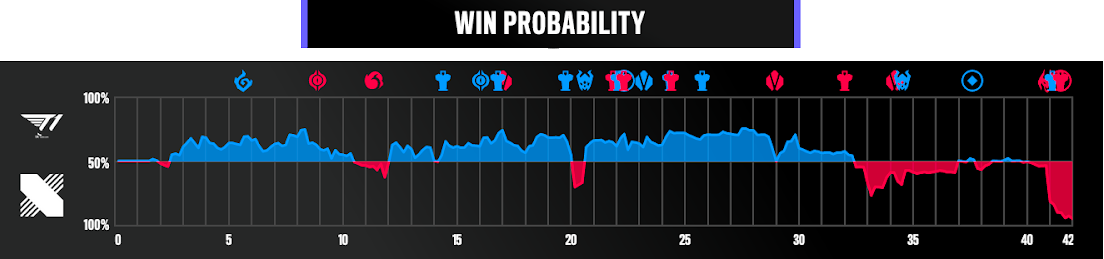
\includegraphics[width=\textwidth]{./images/win_prob_worlds.png}
\caption{Output of the proprietary win prediction model developed by Riot Games from the final game of the 2022 World championships. It shows the winning probability for each team on the y-axis from 100\% for the first team to 100\% for the second team. The icons at the top of the graph are important events during the game and the icons on the left side are the team logos.\cite{LoLEsports}}
\label{fig:riot_win_pred_graph}
\end{figure}


\section*{League of Legends}
\label{sec:LoL}

\Ac{lol} is played with 5 players on each team on a map which is bifurcated into two bases, each linked by three lanes and housing a crucial structure called the \textit{nexus}, which is protected by turrets. 
The game's primary goal is to destroy the opposing team's nexus.
The map includes a jungle area in between the lanes with neutral monsters and two significant creatures, Baron Nashor and the Dragon, offering team-wide benefits when defeated.
Players must accumulate gold and \ac{xp} through defeating minions, neutral monsters, or enemy champions. 
These in-game currencies are essential for purchasing items and levelling up, thereby augmenting a champion's capabilities.

Player roles in \ac{lol} are typically assigned with one player in the top lane, one in the mid lane, two in the bottom lane, and one in the jungle, facilitating strategic diversity and role specialization.
Players select from a roster of 165 champions, each with unique abilities and characteristics, to compete in matches.
Champion selection is a pivotal element of \ac{lol} gameplay, requiring players to consider team composition, damage types, assigned roles, and personal proficiency with specific champions. 
The theoretical number of possible champion combinations in a game is $\binom{165}{10} = \num{3.21e15}$.
Although this number is quite a bit smaller in reality as not every champion can play every role and most players are only really proficient with a handful of champions, this underscores the game's strategic depth.

Each year, \ac{lol} introduces a new 'season', bringing substantial changes, and Riot Games issues bi-weekly patches to adjust champion balance, influencing the prevailing game strategies, or 'meta'.
These patches can also include the release of a new champion or the rework of an old one.
Frequent changes force players to be able to quickly adapt and learn new champions and mechanics.

To evaluate player skill, \ac{lol} utilizes a proprietary rating system, commonly assumed to be a modified Elo system \cite{janssonNeuralNetworksStandardizing2022}.
This system ensures that players are matched with and against others of comparable skill levels, maintaining competitive balance and fairness in the game.

\chapter{Related work}
\label{chap:related}

The application of machine learning techniques in interpreting data from esports games represents a dynamic field of research. 
A critical factor in win prediction is the timing of data collection, as outlined in Table \ref{tab:related_work_lol}.
It can be categorized into three distinct phases: pre-game, in-game, and post-game, each offering unique insights and benefits.

\paragraph{Pre-Game Win Prediction}
A variety of different methods were used to predict the winner prior to the game's commencement.
A notable study by \citeauthor{whiteScalablePsychologicalMomentum2020} \cite{whiteScalablePsychologicalMomentum2020} incorporated a broad spectrum of pre-game features, including the concept of psychological momentum, and attained an accuracy of 0.721 using logistic regression.
In comparison, \citeauthor{doUsingMachineLearning2021} \cite{doUsingMachineLearning2021} 
limited their feature set to player-champion win rates and champion mastery points, further extracting statistical features such as the team's average player-champion win rate.
Applying an \ac{ann} to this data yielded an accuracy of 0.751, which is significant given the relatively small dataset used. 
Especially considering the results of the paper on feature selection by  \citeauthor{costaFeatureAnalysisLeague2021} \cite{costaFeatureAnalysisLeague2021}, which identified not only player-champion win rate but also the kill-to-death ratio for the chosen champion as the most critical features.
These results lead to the assumption that lower rated games are harder to predict accurately, as more mistakes happen and thus increase randomness and volatility.

\paragraph{In-Game Win Prediction}
\Citeauthor{silvaContinuousOutcomePrediction2018} \cite{silvaContinuousOutcomePrediction2018} trained a \acf{rnn} on 7621 professional games  utilizing data from varying intervals, ranging from the initial 0-5 minutes to 20-25 minutes.
Their findings revealed an accuracy of 0.752 when using data from between the 10 and 15 minute mark and a maximum accuracy of 0.835 when using data from the 20-25th minute.
Additionally, their research comparing \ac{lstm} networks against \acp{rnn} indicated superior performance of the latter, possibly attributable to the less complex nature of the problem or limited data availability.
Unfortunately, the work done by Riot Games themselves \cite{claytorRiotGamesAWS2023} did not report any metrics, so no direct comparison to other methods is possible.
\citeauthor{baileyStatisticalLearningEsports} \cite{baileyStatisticalLearningEsports} have achieved an accuracy of 0.77 by applying logistic regression to 671 professional matches with data from the 15th minute mark.

This work builds upon the methodology used by  \Citeauthor{silvaContinuousOutcomePrediction2018} \cite{silvaContinuousOutcomePrediction2018}, but uses a much larger amount of non-professional games in order to overcome any limitations related to the amount of data used.

\paragraph{Post-Game Win Prediction}
\citeauthor{bahrololloomiESportsPlayerPerformance2023} \cite{bahrololloomiESportsPlayerPerformance2023} have built a predictor using post-game data from professional matches achieving 86\% accuracy, while \citeauthor{aniVictoryPredictionLeague2019} \cite{aniVictoryPredictionLeague2019} trained a Random Forest model on a mixture of pre-, in- and post-game data for a maximum accuracy of 0.998.
These results suggest that using post-game data leads to perfect predictions, where the value does not lie in the accuracy, but in the relevant features which can lead to new insights about winning strategies.



\begin{longtblr}[
caption = {Comparison of different works on League of Legends win prediction},
label = {tab:related_work_lol},
note{a} = {No accuracy reported.},
note{b} = {The exact number of features is unclear.},
note{c} = {The exact timestamp where the last in-game data was obtained is unclear.},
note{d} = {The skill group(s) from which the games stem is unclear.},
note{e} = {All professional \ac{lol} games since early 2020 \cite{LoLEsports}.}
]
{
colspec = {l*{5}{c}},
rowhead = 1,
}

Author & Games & Features & Time & Skill Group & Accuracy \\
\hline
\citeauthor{doUsingMachineLearning2021} \cite{doUsingMachineLearning2021} & 5,000 & 44 & pre-game & \TblrNote{d} & 0.751 \\
\citeauthor{costaFeatureAnalysisLeague2021} \cite{costaFeatureAnalysisLeague2021} & 2,840 & 50 & pre-game & professional & \TblrNote{a} \\
\citeauthor{whiteScalablePsychologicalMomentum2020} \cite{whiteScalablePsychologicalMomentum2020}&87,743&\TblrNote{b}&pre-game &equidistributed&0.721\\
\citeauthor{hitar-garciaMachineLearningMethods2023} \cite{hitar-garciaMachineLearningMethods2023} & 7583 & 26 & pre-game & professional & 0.683 \\
\citeauthor{linLeagueLegendsMatch2016} \cite{linLeagueLegendsMatch2016} & 588 & 2231 & pre-game & low-skilled & 0.567 \\

\citeauthor{kimConfidenceCalibratedMOBAGame2020} \cite{kimConfidenceCalibratedMOBAGame2020} & 93875 & 295 & in-game\TblrNote{c} & \TblrNote{d} & 0.738 \\
\citeauthor{shenMachineLearningApproach2022} \cite{shenMachineLearningApproach2022} & 10,000 & 5 & 10 min & \TblrNote{d} & 0.726 & \\
\citeauthor{zhangPredictionEsportsGame2021} \cite{zhangPredictionEsportsGame2021} & 10,000 & 38 & 10 min & high-skilled & 0.723 \\
\citeauthor{baileyStatisticalLearningEsports} \cite{baileyStatisticalLearningEsports} & 671 & 28 & 15 min & professional & 0.76 \\
\citeauthor{silvaContinuousOutcomePrediction2018} \cite{silvaContinuousOutcomePrediction2018} & 7,621 & 52 & 25 min & professional & 0.835 \\
\citeauthor{claytorRiotGamesAWS2023} \cite{claytorRiotGamesAWS2023}  & \TblrNote{e} & 24 & in-game\TblrNote{c} & professional & \TblrNote{a} \\ 

\citeauthor{mondalDoesSupportRole2022} \cite{mondalDoesSupportRole2022} & 296 & 5 & post game & \TblrNote{d} & \TblrNote{a} \\
\citeauthor{bahrololloomiESportsPlayerPerformance2023} \cite{bahrololloomiESportsPlayerPerformance2023} & 2,901 & 15 & post-game & \TblrNote{d} &0.86 \\
\citeauthor{aniVictoryPredictionLeague2019} \cite{aniVictoryPredictionLeague2019} & 1,500 & 97 & post-game & professional & 0.955 \\
\citeauthor{linLeagueLegendsMatch2016} \cite{linLeagueLegendsMatch2016} & 3000 &  \TblrNote{b} & post-game & Gold & 0.936 \\
\hline
\end{longtblr}


\chapter{Technical Background}
\label{chap:background}

This work utilizes a variety of different methods, including \ac{gbt} for feature selection and \ac{rnn}/\ac{gru} for win prediction.
These methods are presented in the following chapter.

\section{Neural Networks}
\label{sec:nn}

\Acp{ann} are computational models that emulate the processing patterns of the human brain. The fundamental computational unit of an ANN is the neuron, a concept first proposed by \citeauthor{mccullochLogicalCalculusIdeas1943} \cite{mccullochLogicalCalculusIdeas1943}.
A neuron computes an output activation $a$ from a set of input values $\mathbf{x} = (x_1, x_2, \ldots, x_m)$, where $m$ denotes the number of inputs. 
The neuron's weighted input $z$ is calculated as the dot product of the input vector $\mathbf{x}$ and the weight vector $\mathbf{w} = (w_1, w_2, \ldots, w_m)$, plus a bias term $b$:
\begin{equation}
z = \sum_{i=1}^{m} w_i x_i + b = \mathbf{w}^\top \mathbf{x} + b.
\end{equation}
The weighted sum $z$ is then passed through an activation function $\phi$, such as a sigmoid or \ac{relu}, to introduce non-linearity:
\begin{equation}
a = \phi(z) = \phi(\mathbf{w}^\top \mathbf{x} + b).
\end{equation}

The \ac{mlp}, introduced by \citeauthor{rosenblattPerceptronProbabilisticModel1958} \cite{rosenblattPerceptronProbabilisticModel1958}, organizes neurons into layers. 
Data flows from the input layer, through one or more hidden layers, to the output layer. In a fully connected feed-forward network, the computation in each layer $l$ is:
\begin{equation}
\mathbf{z}^{(l)} = \mathbf{W}^{(l)} \mathbf{a}^{(l-1)} + \mathbf{b}^{(l)},
\label{eq:ann_zl}
\end{equation}
where $\mathbf{a}^{(l-1)}$ represents the activation of the previous layer, $\mathbf{W}^{(l)}$ the weight matrix, and $\mathbf{b}^{(l)}$ the bias vector of layer $l$.
The vector $\mathbf{z}^{(l)}$ is then passed through the activation function for layer $l$, which is applied elementwise:
\begin{equation}
\mathbf{a}^{(l)} = \phi (\mathbf{z}^{(l)}).
\label{eq:ann_yhat}
\end{equation}
The output layer $L$ produces the network's prediction $\mathbf{\hat{y}}$.
The choice of activation function is dependent on the task, a common choice for classification is the softmax function \cite{bridleProbabilisticInterpretationFeedforward1990}:
\begin{equation}
\label{eq:softmax}
 S(\mathbf{x}_i) = \frac{e^{x_i}}{\sum_{k=1}^{K} e^{x_k}},
\end{equation}
where $K$ is the number of classes and $i = 1, ..., K$.
The softmax function returns a probability distribution over the predicted output classes.

To approximate any measurable function, an \ac{ann} requires at least one hidden layer \cite{hornikMultilayerFeedforwardNetworks1989}. 
The network's weights and biases are adjusted during training to minimize a loss function $E$.
Common loss functions include \ac{mse} for regression tasks:
\begin{equation}
E_N = \frac{1}{N} \sum_{k=1}^{N}(y_{k} - \hat{y}_{k})^2,
\end{equation}
and \ac{cel} for multi-class classification tasks:
\begin{equation}
E_N = -\frac{1}{N} \sum_{n=1}^{N} \sum_{k=1}^{K} y_{nk} \log (\hat{y}_{nk}),
\end{equation}
where $N$ is the number of samples, $y_{nk}$ is the (one-hot encoded) ground truth and $\hat{y}_{nk}$ is the softmax output of sample $n$ and class $k$.

Backpropagation \cite{rumelhartLearningRepresentationsBackpropagating1986} is a key algorithm for training \acp{ann}, involving a forward pass to compute activations and a backward pass to compute gradients. 
The gradients of the loss function with respect to the weights and biases are computed using the chain rule of calculus. For a given layer $l$, the gradient of the loss $E$ with respect to the weights $\mathbf{W}^{(l)}$ is
\begin{equation}
\Delta
\frac{\partial E}{\partial \mathbf{W}^{(l)}} = \frac{\partial E}{\partial \mathbf{a}^{(l)}} \cdot \frac{\partial \mathbf{a}^{(l)}}{\partial \mathbf{z}^{(l)}} \cdot \frac{\partial \mathbf{z}^{(l)}}{\partial \mathbf{W}^{(l)}},
\end{equation}
and with respect to the bias $\mathbf{b}^{(l)}$
\begin{equation}
\frac{\partial E}{\partial \mathbf{b}^{(l)}} = \frac{\partial E}{\partial \mathbf{z}^{(l)}} \cdot \frac{\partial \mathbf{z}^{(l)}}{\partial \mathbf{b}^{(l)}} = \frac{\partial E}{\partial \mathbf{z}^{(l)}}
\end{equation}
as 
\begin{equation}
\frac{\partial \mathbf{z}^{(l)}}{\partial \mathbf{b}^{(l)}} = 1.
\end{equation}
The gradients are then used to update the weights and biases, typically using an optimization algorithm like gradient descent, where the weights are updated via:
\begin{equation}
\mathbf{W}^{(l)} = \mathbf{W}^{(l)} - \eta \frac{\partial E}{\partial \mathbf{W}^{(l)}}
\end{equation}
with $\eta$ being the learning rate.

Through iterative forward and backward propagation, the network gradually converges to a state where the loss is minimized, indicating successful learning of the patterns in the data.

\section{Recurrent Neural Networks}
\label{sec:rnn}

\Ac{rnn} extend the capabilities of feed-forward neural networks to handle sequential data by introducing the concept of recurrence. 
In an \ac{rnn}, the output at each time step is influenced not only by the current input but also by the network's previous internal state, known as the hidden state. 
This design enables \acp{rnn} to capture temporal dependencies, making them particularly effective for tasks involving sequential data, such as speech recognition and natural language processing \cite{lecunDeepLearning2015}.
The concept of a fully connected \ac{rnn} was first proposed by \citeauthor{elmanFindingStructureTime1990} \cite{elmanFindingStructureTime1990}.

\Acp{rnn} maintain a 'state vector' in their hidden units, which implicitly contains information extracted from all past elements of the sequence \cite{lecunDeepLearning2015}.
Compared to vanilla \acp{ann}, the \ac{rnn} has three weight matrices $\mathbf{W}$, $\mathbf{V}$ and $\mathbf{U}$, which represent input-to-hidden, hidden-to-output and temporal connections (see Figure \ref{fig:rnn_unroll}).
These matrices are shared across timesteps.
The hidden state $\mathbf{h}_t$ at time step $t$ is updated as follows:
\begin{equation}
\label{eq:rnn_update} 
\mathbf{h}_t =
\begin{cases}
	0, & \text{if } t = 0, \\
	\sigma_h (\mathbf{W} \mathbf{x}_t + \mathbf{U} \mathbf{h}_{t-1} + \mathbf{b}_h)
	& \text{otherwise},
\end{cases}
\end{equation}
where $\mathbf{U}$ is the weight matrix for the hidden state and $\mathbf{W}$ is the weight matrix for the input.
A common choice for $\sigma_h$ is the tanh function.
The output $\mathbf{\hat{y}}_t$ of an \ac{rnn} at time step $t$ can be calculated similar to (\ref{eq:ann_zl}) and (\ref{eq:ann_yhat}) with:
\begin{equation}
\label{eq:rnn_output}
\begin{split}
\mathbf{o}_t &= \mathbf{V} \cdot \mathbf{h}_t + \mathbf{b}_h \\
\mathbf{\hat{y}}_t &= S(\mathbf{o}_t)
\end{split}
\end{equation}
where $\mathbf{V}$ is the weight matrix associated with the cell output and $S$ the softmax function defined in (\ref{eq:softmax}). 

The loss over $T$ timesteps is defined by 
\begin{equation}
E_T = \frac{1}{T} \sum_{t=1}^{T} {l(\mathbf{\hat{y}}_t, \mathbf{y})}
\end{equation} 
%TODO: consider changing l to e
where $l(\mathbf{\hat{y}}_t, \mathbf{y})$ is the loss at timestep $t$.

\Ac{bptt} unfolds the \ac{rnn} across time steps (see Figure \ref{fig:rnn_unroll}) and applies the backpropagation algorithm. 
In order to train the weight matrices, we need the partial derivatives of $E_T$ with respect to $\mathbf{U}$, $\mathbf{V}$ and $\mathbf{W}$.

As the weight matrices are shared across timesteps, we can generally sum up the gradients from each timestep $t$.
The gradient of the loss function with regards to the output matrix $\mathbf{V}$ does not depend on the hidden state $\mathbf{h}_t$ and can thus be calculated easily:
\begin{equation}
\label{eq:bptt_V}
\begin{split}
\frac{\partial E_T}{\partial \mathbf{V}} 
& = 
\sum_{t}^{T} \frac{\partial E_t}{\partial \mathbf{V}} \\
& =
\sum_{t}^{T} 
\frac{\partial E_t}{\partial \mathbf{\hat{y}}_t} 
\cdot 
\frac{\partial \mathbf{\hat{y}}_t}{\partial \mathbf{o}_t} 
\cdot 
\frac{\partial \mathbf{o}_t}{\partial \mathbf{V}}.
\end{split}
\end{equation}
Now we consider the gradient with respect to the weight matrix for the hidden state $U$ at the time step $t+1$:
\begin{equation}
\frac{\partial E_{t+1}}{\partial \mathbf{U}} = 
\frac{\partial E_{t+1}}{\partial \mathbf{\hat{y}}_{t+1}}
\frac{\partial \mathbf{\hat{y}}_{t+1}}{\partial \mathbf{h}_{t+1}}
\frac{\partial \mathbf{h}_{t+1}}{\partial \mathbf{U}}.
\end{equation}
As the hidden state $h_{t+1}$ depends on the hidden state of the previous timestep $h_t$, we need to recursively calculate the partial derivatives of all the previous timesteps, yielding the following formula:
\begin{equation}
\frac{\partial E_{t+1}}{\partial \mathbf{U}} = \sum_{k=1}^{t+1}
\frac{\partial E_{t+1}}{\partial \mathbf{\hat{y}}_{t+1}}
\frac{\partial \mathbf{\hat{y}}_{t+1}}{\partial \mathbf{h}_{t+1}}
\frac{\partial \mathbf{h}_{t+1}}{\partial \mathbf{h}_k}
\frac{\partial \mathbf{h}_k}{\partial \mathbf{U}}.
\end{equation}
Applying the chain rule to $\frac{\partial \mathbf{h}_{t+1}}{\partial \mathbf{h}_k}$ yields
\begin{equation}
\frac{\partial E_{t+1}}{\partial \mathbf{U}} = \sum_{k=1}^{t+1}
\frac{\partial E_{t+1}}{\partial \mathbf{\hat{y}}_{t+1}}
\frac{\partial \mathbf{\hat{y}}_{t+1}}{\partial \mathbf{h}_{t+1}}
\left(\prod_{j=k}^{t}\frac{\partial \mathbf{h}_{j+1}}{\partial \mathbf{h}_j}\right)
\frac{\partial \mathbf{h}_k}{\partial \mathbf{U}}
\end{equation}\cite{aratBackpropagationTimeRecurrent2019}.
Summing the partial derivatives over timesteps similar to (\ref{eq:bptt_V}) yields the full equation
\begin{equation}
\label{eq:bptt_U}
\frac{\partial E_T}{\partial \mathbf{U}} = 
\sum_{t=1}^{T}
\sum_{k=1}^{t}
\frac{\partial E_{t+1}}{\partial \mathbf{\hat{y}}_{t+1}}
\frac{\partial \mathbf{\hat{y}}_{t+1}}{\partial \mathbf{h}_{t+1}}
\frac{\partial \mathbf{h}_{t+1}}{\partial \mathbf{h}_k}
\frac{\partial \mathbf{h}_k}{\partial \mathbf{U}},
\end{equation}
where
\begin{equation}
\label{eq:bptt_ht+1}
\frac{\partial \mathbf{h}_{t+1}}{\partial \mathbf{h}_k} 
= 
\left(\prod_{j=k}^{t}\frac{\partial \mathbf{h}_{j+1}}{\partial \mathbf{h}_j}\right)
=
\frac{\partial \mathbf{h}_{t+1}}{\partial \mathbf{h}_t}
\frac{\partial \mathbf{h}_{t}}{\partial \mathbf{h}_{t-1}}
 . . . 
\frac{\partial \mathbf{h}_{k+1}}{\partial \mathbf{h}_k}.
\end{equation}
The gradient with respect to $\mathbf{W}$ follows similarly.
As first demonstrated by \citeauthor{bengioLearningLongtermDependencies1994} \cite{bengioLearningLongtermDependencies1994}, RNNs face challenges with exploding or vanishing gradients, particularly in long sequences.

This can be shown by examining a single term from (\ref{eq:bptt_ht+1}) as this is the partial derivative between two vectors and as such a Jacobian matrix of the transition from $\mathbf{h}_t$ to $\mathbf{h}_{t+1}$:
\begin{equation}
\label{eq:bptt_jacobian}
\frac{\partial \mathbf{h}_{j+1}}{\partial \mathbf{h}_j}
= 
\text{diag}(\sigma_{h}' ( \mathbf{U} \mathbf{h}_j + \mathbf{b}_h)) \mathbf{U}
\end{equation}
where diag() converts a vector into a diagonal matrix and $\sigma '$ computes the element-wise derivative of $\sigma$
\cite{pascanuDifficultyTrainingRecurrent2013}.
The eigendecomposition of $\frac{\partial \mathbf{h}_{j+1}}{\partial \mathbf{h}_j}$ yields the eigenvalues $ \lambda_1, \lambda_2, ..., \lambda_n$ where $|\lambda_1| > |\lambda_2| > ... > |\lambda_n|$ with their corresponding eigenvectors $v_1, v_2, ..., v_n$.
The change in hidden state $\Delta h_{j+1}$ in direction of a vector $v_i$ is multiplied with the corresponding eigenvalue: $\lambda_i \Delta h_{j+1}$.
As these factors are multiplied across timesteps, the change is scaled by a factor equivalent to $\lambda_i^t$ which scales exponentially with the timestep $t$.
If $\lambda_1 < 1$ the gradient will vanish while if $\lambda_1 > 1$ the gradient will explode when considering $t \to \infty$ \cite{pascanuDifficultyTrainingRecurrent2013}.
This issue hinders their ability to learn long-range dependencies \cite{sutskeverTrainingRecurrentNeural2013}. 

\begin{figure}
\centering
\begin{tikzpicture}[
item/.style={circle,draw,thick,align=center, minimum size=1.2cm},
hidden/.style={item,on chain,join}]

 \begin{scope}[start chain=going right,nodes=hidden,every
 join/.style={-latex,very thick},local bounding box=chain]
 \draw node (A0) {$\mathbf{h}_0$} node (A1) {$\mathbf{h}_1$} node (A2) {$\mathbf{h}_2$} node[xshift=2em] (At)
 {$\mathbf{h}_t$};
 \end{scope}
 \node[left=1em of chain,scale=2] (eq) {$=$};
 \node[left=2em of eq,item] (AL) {$\mathbf{h}$};
 \path (AL.west) ++ (-1em,2em) coordinate (aux);
 \draw[very thick,-latex,rounded corners] (AL.east) -| ++ (1em,2em) -- (aux) --++(0em,-2em) node[midway, left] {$\mathbf{U}$} -- (AL.west); 
 \foreach \X in {0,1,2,t}
 {\draw[very thick,-latex] (A\X.north) -- ++ (0,2em) node[midway, right] {$\mathbf{V}$}
 node[above,item,fill=gray!10] (h\X) {$\mathbf{\hat{y}}_\X$};
 \draw[very thick,latex-] (A\X.south) -- ++ (0,-2em) node[midway, right] {$\mathbf{W}$}
 node[below,item,fill=gray!10] (x\X) {$\mathbf{x}_\X$};
 \path (A0.east) -- (A1.west) node[midway, above] {$\mathbf{U}$};
 \path (A1.east) -- (A2.west) node[midway, above] {$\mathbf{U}$};
 \path (A2.east) -- (At.west) node[midway, above] {$\mathbf{U}$};
}
 
 \draw[white,line width=0.8ex] (AL.north) -- ++ (0,1.9em);
 \draw[very thick,-latex] (AL.north) -- ++ (0,2em) node[midway, right] {$\mathbf{V}$}
 node[above,item,fill=gray!10] {$\mathbf{\hat{y}}_t$};
 \draw[very thick,latex-] (AL.south) -- ++ (0,-2em) node[midway, right] {$\mathbf{W}$}
 node[below,item,fill=gray!10] {$\mathbf{x}_t$};
 \path (x2) -- (xt) node[midway,scale=2,font=\bfseries] {\dots};
\end{tikzpicture}
\caption{Unrolling of an \ac{rnn} over time by creating a copy of the model for each time step $t$ with shared weight matrices, where $\mathbf{U}$ is the matrix representing the recurrent connection and the grey nodes containing $\mathbf{x}_t$ and $\mathbf{\hat{y}}_t$ are the input and output at timestep $t$.}
\label{fig:rnn_unroll}
\end{figure}

\section{Gated Recurrent Unit}
\label{sec:gru}
In order to overcome the exploding/vanishing gradient problem of vanilla \acp{rnn}, gated networks like the \ac{lstm} \cite{hochreiterLongShortTermMemory1997} and \ac{gru} \cite{choLearningPhraseRepresentations2014} have been developed \cite{vanhoudtReviewLongShortterm2020}.
As they introduce an increased number of parameters compared to traditional \acp{rnn}, gated networks like the \ac{lstm} and \ac{gru} demand greater computational power \cite{deyGatevariantsGatedRecurrent2017}.
Gating mechanisms mitigate the exploding/vanishing gradient problem by regulating how much the hidden state is updated each step.
Compared to the \ac{lstm} network, \ac{gru} reduces the number of gate networks to two, thus being simpler to implement and compute \cite{choLearningPhraseRepresentations2014} (see Figure \ref{fig:gru}).
\Citeauthor{chungEmpiricalEvaluationGated2014} even found that \ac{gru} is at least comparable to \ac{lstm} in most cases \cite{chungEmpiricalEvaluationGated2014}.
The gates control the activation of each hidden unit.
The reset gate $\mathbf{r}_t$ is calculated by
\begin{equation}
\label{eq:gru_reset}
\mathbf{r}_t = \sigma (\mathbf{W}_r \mathbf{x}_t + \mathbf{U}_r \mathbf{h}_{t-1})
\end{equation}
and the update gate $\mathbf{z}_t$ by
\begin{equation}
\label{eq:gru_update}
\mathbf{z}_t = \sigma (\mathbf{W}_z \mathbf{x}_t + \mathbf{U}_z \mathbf{h}_{t-1})
\end{equation}
\cite{deyGatevariantsGatedRecurrent2017}.
The hidden state update is a linear interpolation between the previous activation $\mathbf{h}_{t-1}$ and the candidate activation $\mathbf{\tilde{h}}_t$, where the update gate $\mathbf{z}_t$ influences how much the hidden state is changed \cite{chungEmpiricalEvaluationGated2014}:
\begin{equation}
\label{eq:gru_h}
\mathbf{h}_t = (1-\mathbf{z}_t) \odot \mathbf{\tilde{h}}_t + \mathbf{z}_t \odot \mathbf{h}_{t-1} 
\end{equation}
with
\begin{equation}
\label{eq:gru_h_tilde}
\mathbf{\tilde{h}}_t = \tanh(\mathbf{W}_h \mathbf{x}_t + \mathbf{U}_h (\mathbf{r}_t \odot \mathbf{h}_{t-1})).
\end{equation}
In equations (\ref{eq:gru_h}) and (\ref{eq:gru_h_tilde}) $\odot$ denotes the element-wise (Hadamard) multiplication.
Equation \ref{eq:gru_h} shows that if $\mathbf{z}_t$ is close to one, previous memory in $\mathbf{h}_{t-1}$ is propagated to $\mathbf{h}_t$ and the model learns long-term dependencies.
Conversely, if $\mathbf{r}_t$ is active and $\mathbf{z}_t$ is not, the hidden state gets updated with information from the last step, thus learning short-term dependencies.
This selective inclusion of new information and the ability to skip a timestep completely can help mitigate the exploding / vanishing gradient problem described in Section \ref{sec:rnn}.

\begin{figure}
\centering
\begin{tikzpicture}[
    % Styles
    cell/.style={% For the main box
        rectangle, 
        rounded corners=5mm, 
        draw,
        very thick,
        },
    operator/.style={%For operators like +  and  x
        circle,
        draw,
        inner sep=0.5pt,
        minimum height =.2cm,
        },
    function/.style={%For functions
        ellipse,
        draw,
        inner sep=3pt
        },
    ct/.style={% For external inputs and outputs
        circle,
        draw,
        line width = .75pt,
        minimum width=1cm,
        inner sep=1pt,
        },
    gt/.style={% For internal inputs
        rectangle,
        draw,
        minimum width=4mm,
        minimum height=3mm,
        inner sep=3pt
        },
    ArrowC1/.style={% Arrows with rounded corners
        rounded corners=.25cm,
        thick,
        },
    ArrowC2/.style={% Arrows with big rounded corners
        rounded corners=.5cm,
        thick,
        },
    ]
    
   %Start drawing the thing...    
    % Draw the cell: 
    \node [cell, minimum height =4cm, minimum width=6cm] at (0,0){} ;
    
    
	%Draw operators	
	%top row
	\node [operator] (mux1) at (0,1.5) {$\times$};
    \node [operator] (add1) at (2,1.5) {$+$};
    %second row
    \node [operator] (mux2) at (-2, 0.5) {$\times$};
    \node [operator] (mux3) at (2,  0.5) {$\times$};
    \node [operator, inner sep=0pt] (minus) at (1, 0.5) {
    \begin{scriptsize}
    $1-$
    \end{scriptsize}
    };
    %bottom row
    \node [gt] (sigma1) at (-1.5, -0.5) {$\sigma$};
    \node [gt] (sigma2) at (0, -0.5) {$\sigma$};
    \node [gt] (tanh) at (2, -0.5) {$\tanh$};
    
    %draw node to show location of gates
    \node[] (zt) at (1, -0.5) {$\mathbf{z}_t$};
    \node[]  (rt) at (-1, 0) {$\mathbf{r}_t$};
    
  % Draw External inputs
    \node[] (ht-1) at (-4,1.5) {$\mathbf{h}_{t-1}$};
    \node[outer sep=1] (xt) at (-2.5,-3) {$\mathbf{x}_t$};

    % Draw External outputs
    \node[] (out) at (4,1.5) {$\mathbf{h}_t$};
    \node[] (ht) at (2.5,3) {$\mathbf{\hat{y}}_t$};
    
   % Draw Arrows
   % input
	\draw [ArrowC2] (ht-1) -- (mux1) ;
	\draw [->, ArrowC1] (ht-1) -| (mux2);
	\draw[->, ArrowC1] (ht-1) -| (-2.5, -1) -| (sigma1);
	\draw[->, ArrowC1] (xt.north) -| (-2.5, -1) -| (sigma1);
	\draw[->, ArrowC1] (xt.north) |- (-1.5, -1.5) -|(tanh);
	\draw[->, ArrowC1] (xt.north) -| (-2.5, -1) -| (sigma2);
   
	% Internal   
	\draw[->, ArrowC1] (mux1) -- (add1) -- (out);
	\draw[ArrowC1] (mux2) |- (-1,-1.5); 
	\draw[->, ArrowC1] (sigma1) |- (mux2);
	\draw[->, ArrowC1] (sigma2) -- (mux1);
	\draw[->, ArrowC1] (sigma2) |- (minus);
	\draw[->, ArrowC1] (minus) -- (mux3);
	\draw[->, ArrowC1] (tanh) -- (mux3);
	\draw[->, ArrowC1] (mux3) -- (add1);
   
   %Output
   \draw[->, ArrowC1] (add1) -| (ht);
    
\end{tikzpicture}
\caption{Gated Recurrent Unit}
\label{fig:gru}
\end{figure}


\section{Feature Selection}
\label{sec:fs_algos}

Feature Selection is pivotal in machine learning, particularly when dealing with high-dimensional data. It serves the primary objectives of improving model performance by mitigating the 'curse of dimensionality,' enhancing predictive accuracy, and reducing overfitting. By eliminating irrelevant or redundant features, the model's generalization capacity is enhanced, contributing to model interpretability and potentially reducing training times.
Feature selection methods can be broadly categorized into three distinct types \cite{jovicReviewFeatureSelection2015}:
\begin{description}

\item[Filter Methods] These methods rely on model-invariant information, such as feature-class label correlation. They are computationally efficient and typically do not require user input in form of hyperparameters, but may not capture complex relationships within the data.

\item[Wrapper Methods] Models are trained iteratively on various feature subsets, incurring a higher computational cost but enabling the detection of interactions among variables \cite{venkateshReviewFeatureSelection2019}.

\item[Embedded Methods] These methods perform inherent feature selection, often as an integral part of the modeling process. Tree-based models, such as Decision Trees and \ac{gbt}, typically employ feature selection based on metrics like the Gini index or entropy.
\end{description}

The two methods used in this work are a filter method (\ac{pcc}) and an embedded method (\ac{gbt}) and are presented in more detail below.


\subsection*{Pearson's Correlation Coefficient}
\label{ssec:pearsons}
\Ac{pcc} is a statistical measure widely used to evaluate the linear relationship between two variables. 
Specifically, we consider its application in the context of feature selection in machine learning, where it is used to assess the linear correlation between input features and the target variable. 
We regard the input vector $\mathbf{x}$ as a manifestation of an underlying, unknown distribution. 
Here, $X_i$ represents the random variable corresponding to the $i^{\text{th}}$ component of $\mathbf{x}$, and $y$ is the target value, viewed as a realization of the random variable $Y$ \cite{guyonIntroductionVariableFeature2003}. 
\Ac{pcc} is employed to quantify the linear correlation between these two random variables. It is defined by the formula:
\begin{equation}
R(i) = \frac{\text{cov}(X_i, Y)}{\sqrt{\text{var}(X_i) \cdot \text{var}(Y)}},
\end{equation}
where $\text{cov}(X_i, Y)$ is the covariance between $X_i$ and $Y$, and $\text{var}(X_i)$ and $\text{var}(Y)$ are the variances of $X_i$ and $Y$, respectively \cite{chandrashekarSurveyFeatureSelection2014}.
$R(i) \in [-1; +1]$ where -1 and +1 are strong negative or positive correlations and 0 indicates no correlation. 
A hypothesis test should be performed in order to ascertain the significance of the test results, with the null hypothesis that there is no correlation between the feature and the target.
As it is a non-parametric model, there is no need to tune hyperparameters or risk of overfitting.
While simple and effective for identifying linear relationships, \ac{pcc} only captures linear dependencies and might miss non-linear relationships crucial for neural networks.
Despite these limitations, \ac{pcc} is a valuable tool in feature selection for its simplicity and efficiency in revealing linear correlations.

\subsection*{Gradient Boosted Trees}
\label{ssec:gbt}

\Ac{gbt} is an ensemble learning technique that can be used for feature selection. 
The core idea of \ac{gbt} is to build a model in a stage-wise fashion, where each tree incrementally improves upon the previous ones by correcting their errors. 
This process involves training trees sequentially, with each new tree learning to predict the residuals or errors of the previous ensemble of trees.

The mathematical foundation of \ac{gbt} can be described through the framework of additive models. 
Given a dataset with \(n\) instances \((x_i, y_i)\), where \(x_i\) represents the feature vector of the \(i\)-th instance and \(y_i\) is its corresponding target value, the goal of \ac{gbt} is to find an approximation \(\hat{F}(x)\) to the true function \(F(x)\) that minimizes the expected value of some specified loss function \(L(y, F(x))\). 
\Ac{gbt} models build an approximation of $F(x)$ as the weighted sum of the functions
\begin{equation}
F_m(x) = F_{m-1}(x) + \phi_m h_m(x)
\end{equation}
where $\phi_m$ is the weight of the $m^{th}$ function $h_m(x)$\cite{bentejacComparativeAnalysisGradient2021}.

The \ac{gbt} model is constructed iteratively, starting with a constant model \(F_0(x) = \arg\min_{\gamma} \sum_{i=1}^{n} E(y_i, \gamma)\), and incrementally adding trees to minimize the loss function. 
Each subsequent tree models the residual errors made by the previous ensemble of trees. Specifically, at each stage \(t\), a tree \(h_t(x)\) is fitted to the negative gradient of the loss function
\begin{equation}
-\left[\frac{\partial E(y_i, F(x_i))}{\partial F(x_i)}\right]_{F(x)=F_{t-1}(x)},
\end{equation}
evaluated at the predictions \(F_{t-1}(x)\) of the current model.
The update equation for the model at each stage \(t\) is given by:
\begin{equation}
F_t(x) = F_{t-1}(x) + \nu \cdot h_t(x)
\end{equation}
where \(\nu\) is the learning rate, a parameter that scales the contribution of each tree. 
The learning rate is crucial for the performance of \ac{gbt}, as it controls the speed at which the model learns. 
A smaller \(\nu\) requires more trees to model the data but can lead to a more robust model by reducing the risk of overfitting.

There are different types of importance, such as the average or total gain across all splits the feature is used in.
The simplest definition is the 'weight', defined as the number of times a feature is used to split the data across all trees \cite{chenXGBoostScalableTree2016}.

\chapter{Experiments}
\label{chap:experiments}
This section introduces two distinct experiments designed to evaluate the effectiveness of predictive models in \ac{lol}. The initial experiment centers on pre-game win prediction through a neural network, utilizing historical and statistical data before the game starts. In contrast, the subsequent experiment explores real-time prediction using a \ac{gru} model, aiming to dynamically determine winning probabilities as the game unfolds.

\section{Data}
\label{sec:data}

Building upon the aforementioned approach, two different datasets are used: one dataset containing all relevant information prior to the start of the game and one dataset containing only the temporal information from the beginning of the game.


\subsection{Data Collection}
\label{ssec:datacoll}

The data collection process for this study involved a dual-pronged approach, leveraging the resources provided by the Riot Games API alongside a targeted web-scraping strategy.
The resulting raw dataset, stored in a PostgreSQL Database, reflects a comprehensive compilation of high-rank amateur \acl{lol} matches.

\paragraph{High-Rank Matches}
The rating system in \ac{lol} groups players into different skill groups, where the lowest is 'Iron' and the highest 'Challenger'.
The two highest ranks,'Grandmaster' and 'Challenger' contain the best 300 or 700 best players on each server.
The exact number of players these tiers depend on the player number in each region (see \cite{riotgamesMasterGrandmasterChallenger2023}).

Similar to the methodology of \citeauthor{zhangPredictionEsportsGame2021} \cite{zhangPredictionEsportsGame2021}, the focus of data acquisition was directed towards high-rank matches, in which a mix of excellent amateur and professional players play.
High rank matches in this context are defined as having at least one player holding the rank of Master, Grandmaster or Challenger.
These ranks combined account for the top $0.2\%$ of all players \cite{riotgamesRankedTiersDivisions2023}.
Riot Games themselves considers any rank above Diamond 3 as 'Elite' \cite{riotgamesDevBalanceFramework2020}, but we raise this bar just slightly to only include any rank at Master or above.
Due to the fact that for a match to be included in the dataset, only one out of ten players needs to hold one of the aforementioned highest ranks, some slightly lower ranked players are also present in the dataset.

Lower rank matches are not considered due to their higher unpredictability as less skilled players are assumed to make huge, game-changing mistakes more often.
This higher unpredictability could make it harder for the model to learn.

Pro matches, defined as professional players playing with their respective teams in an esports tournament or league, are not included as they are not available through the official Riot Games API.
Professional players are still included in the dataset, but only if they played regular, non-tournament games.

\paragraph{Riot Games API}
The primary source of data stems from the Riot Games API \cite{RiotDeveloperPortal}, a comprehensive repository of information pertaining to \ac{lol} gameplay.
The Riot Games API provides access to a plethora of essential data points, including champion statistics, general match information, timeline details, and player-specific information.

\paragraph{Other Data Sources}
However, not all pertinent data were available directly from the Riot Games API.
These include the general winning chance of each champion and statistics on how each player performs on each relevant champion.
To address this limitation, additional relevant information was gathered by using web scraping on u.gg \cite{GGBestLeague}.
\paragraph{Regions}
Multiple regions were included in the data collection process, including Europe West (EUW), Europe Nordic \& East (EUN), Korea (KR), and North America (NA).
This regional diversity contributes to the model's generalizability across different player bases and playing styles.
\paragraph{Period of Time}
All matches included in the dataset were played in season 13 and on patch 20.
It is important that all matches are played on the same patch, as a patch may cause major shifts in the balance of the game, thus potentially making certain strategies and champions way better than others.
\\\\
The pre-game dataset encompasses a total of 38,957 matches, while the in-game dataset contains 28,809 matches.
In \ref{ssec:dataprop}, the pre-game dataset characteristics are presented in more detail, as the smaller in-game dataset is a random sampling from the pre-game dataset. 
As it is a random sample, the dataset characteristics are shared. 
The sampling is necessary due to the long processing time of in-game data, necessitating a smaller dataset compared to pre-game data.

\paragraph{Region Distribution}
The dataset is primarily comprised of matches from three major regions: North America, Western Europe, and South Korea, which collectively constitute the vast majority of matches in our dataset. 
It is important to note that due to a lack of official data pertaining to the number of games played or the number of players in each region, it is currently not feasible to conclusively verify whether the distribution of matches within our dataset aligns with the true underlying distribution of games played per region.
The major regions in the dataset are the same regions getting guaranteed spots at the world championship \cite{2023LeagueLegends2023} with the exception of China, whose matches are not available through the Riot Games API.
Consequently, it is reasonable to assume that this composition approximately mirrors the real-world distribution of matches, with the exception of chinese games.
A visual representation of the distribution of matches across regions is provided in Figure \ref{fig:platformId}.


\begin{figure}[ht]
%% Creator: Matplotlib, PGF backend
%%
%% To include the figure in your LaTeX document, write
%%   \input{<filename>.pgf}
%%
%% Make sure the required packages are loaded in your preamble
%%   \usepackage{pgf}
%%
%% Also ensure that all the required font packages are loaded; for instance,
%% the lmodern package is sometimes necessary when using math font.
%%   \usepackage{lmodern}
%%
%% Figures using additional raster images can only be included by \input if
%% they are in the same directory as the main LaTeX file. For loading figures
%% from other directories you can use the `import` package
%%   \usepackage{import}
%%
%% and then include the figures with
%%   \import{<path to file>}{<filename>.pgf}
%%
%% Matplotlib used the following preamble
%%   
%%   \usepackage{fontspec}
%%   \setmainfont{DejaVuSerif.ttf}[Path=\detokenize{/Users/admin/opt/miniconda3/envs/Leaguify/lib/python3.10/site-packages/matplotlib/mpl-data/fonts/ttf/}]
%%   \setsansfont{Arial.ttf}[Path=\detokenize{/System/Library/Fonts/Supplemental/}]
%%   \setmonofont{DejaVuSansMono.ttf}[Path=\detokenize{/Users/admin/opt/miniconda3/envs/Leaguify/lib/python3.10/site-packages/matplotlib/mpl-data/fonts/ttf/}]
%%   \makeatletter\@ifpackageloaded{underscore}{}{\usepackage[strings]{underscore}}\makeatother
%%
\begingroup%
\makeatletter%
\begin{pgfpicture}%
\pgfpathrectangle{\pgfpointorigin}{\pgfqpoint{6.268788in}{4.714041in}}%
\pgfusepath{use as bounding box, clip}%
\begin{pgfscope}%
\pgfsetbuttcap%
\pgfsetmiterjoin%
\definecolor{currentfill}{rgb}{1.000000,1.000000,1.000000}%
\pgfsetfillcolor{currentfill}%
\pgfsetlinewidth{0.000000pt}%
\definecolor{currentstroke}{rgb}{1.000000,1.000000,1.000000}%
\pgfsetstrokecolor{currentstroke}%
\pgfsetdash{}{0pt}%
\pgfpathmoveto{\pgfqpoint{0.000000in}{0.000000in}}%
\pgfpathlineto{\pgfqpoint{6.268788in}{0.000000in}}%
\pgfpathlineto{\pgfqpoint{6.268788in}{4.714041in}}%
\pgfpathlineto{\pgfqpoint{0.000000in}{4.714041in}}%
\pgfpathlineto{\pgfqpoint{0.000000in}{0.000000in}}%
\pgfpathclose%
\pgfusepath{fill}%
\end{pgfscope}%
\begin{pgfscope}%
\pgfsetbuttcap%
\pgfsetmiterjoin%
\definecolor{currentfill}{rgb}{0.917647,0.917647,0.949020}%
\pgfsetfillcolor{currentfill}%
\pgfsetlinewidth{0.000000pt}%
\definecolor{currentstroke}{rgb}{0.000000,0.000000,0.000000}%
\pgfsetstrokecolor{currentstroke}%
\pgfsetstrokeopacity{0.000000}%
\pgfsetdash{}{0pt}%
\pgfpathmoveto{\pgfqpoint{1.715316in}{0.506819in}}%
\pgfpathlineto{\pgfqpoint{6.168788in}{0.506819in}}%
\pgfpathlineto{\pgfqpoint{6.168788in}{4.614041in}}%
\pgfpathlineto{\pgfqpoint{1.715316in}{4.614041in}}%
\pgfpathlineto{\pgfqpoint{1.715316in}{0.506819in}}%
\pgfpathclose%
\pgfusepath{fill}%
\end{pgfscope}%
\begin{pgfscope}%
\pgfpathrectangle{\pgfqpoint{1.715316in}{0.506819in}}{\pgfqpoint{4.453472in}{4.107222in}}%
\pgfusepath{clip}%
\pgfsetroundcap%
\pgfsetroundjoin%
\pgfsetlinewidth{0.803000pt}%
\definecolor{currentstroke}{rgb}{1.000000,1.000000,1.000000}%
\pgfsetstrokecolor{currentstroke}%
\pgfsetdash{}{0pt}%
\pgfpathmoveto{\pgfqpoint{1.715316in}{0.506819in}}%
\pgfpathlineto{\pgfqpoint{1.715316in}{4.614041in}}%
\pgfusepath{stroke}%
\end{pgfscope}%
\begin{pgfscope}%
\definecolor{textcolor}{rgb}{0.150000,0.150000,0.150000}%
\pgfsetstrokecolor{textcolor}%
\pgfsetfillcolor{textcolor}%
\pgftext[x=1.715316in,y=0.409597in,,top]{\color{textcolor}\sffamily\fontsize{10.000000}{12.000000}\selectfont 0}%
\end{pgfscope}%
\begin{pgfscope}%
\pgfpathrectangle{\pgfqpoint{1.715316in}{0.506819in}}{\pgfqpoint{4.453472in}{4.107222in}}%
\pgfusepath{clip}%
\pgfsetroundcap%
\pgfsetroundjoin%
\pgfsetlinewidth{0.803000pt}%
\definecolor{currentstroke}{rgb}{1.000000,1.000000,1.000000}%
\pgfsetstrokecolor{currentstroke}%
\pgfsetdash{}{0pt}%
\pgfpathmoveto{\pgfqpoint{2.292408in}{0.506819in}}%
\pgfpathlineto{\pgfqpoint{2.292408in}{4.614041in}}%
\pgfusepath{stroke}%
\end{pgfscope}%
\begin{pgfscope}%
\definecolor{textcolor}{rgb}{0.150000,0.150000,0.150000}%
\pgfsetstrokecolor{textcolor}%
\pgfsetfillcolor{textcolor}%
\pgftext[x=2.292408in,y=0.409597in,,top]{\color{textcolor}\sffamily\fontsize{10.000000}{12.000000}\selectfont 2500}%
\end{pgfscope}%
\begin{pgfscope}%
\pgfpathrectangle{\pgfqpoint{1.715316in}{0.506819in}}{\pgfqpoint{4.453472in}{4.107222in}}%
\pgfusepath{clip}%
\pgfsetroundcap%
\pgfsetroundjoin%
\pgfsetlinewidth{0.803000pt}%
\definecolor{currentstroke}{rgb}{1.000000,1.000000,1.000000}%
\pgfsetstrokecolor{currentstroke}%
\pgfsetdash{}{0pt}%
\pgfpathmoveto{\pgfqpoint{2.869501in}{0.506819in}}%
\pgfpathlineto{\pgfqpoint{2.869501in}{4.614041in}}%
\pgfusepath{stroke}%
\end{pgfscope}%
\begin{pgfscope}%
\definecolor{textcolor}{rgb}{0.150000,0.150000,0.150000}%
\pgfsetstrokecolor{textcolor}%
\pgfsetfillcolor{textcolor}%
\pgftext[x=2.869501in,y=0.409597in,,top]{\color{textcolor}\sffamily\fontsize{10.000000}{12.000000}\selectfont 5000}%
\end{pgfscope}%
\begin{pgfscope}%
\pgfpathrectangle{\pgfqpoint{1.715316in}{0.506819in}}{\pgfqpoint{4.453472in}{4.107222in}}%
\pgfusepath{clip}%
\pgfsetroundcap%
\pgfsetroundjoin%
\pgfsetlinewidth{0.803000pt}%
\definecolor{currentstroke}{rgb}{1.000000,1.000000,1.000000}%
\pgfsetstrokecolor{currentstroke}%
\pgfsetdash{}{0pt}%
\pgfpathmoveto{\pgfqpoint{3.446594in}{0.506819in}}%
\pgfpathlineto{\pgfqpoint{3.446594in}{4.614041in}}%
\pgfusepath{stroke}%
\end{pgfscope}%
\begin{pgfscope}%
\definecolor{textcolor}{rgb}{0.150000,0.150000,0.150000}%
\pgfsetstrokecolor{textcolor}%
\pgfsetfillcolor{textcolor}%
\pgftext[x=3.446594in,y=0.409597in,,top]{\color{textcolor}\sffamily\fontsize{10.000000}{12.000000}\selectfont 7500}%
\end{pgfscope}%
\begin{pgfscope}%
\pgfpathrectangle{\pgfqpoint{1.715316in}{0.506819in}}{\pgfqpoint{4.453472in}{4.107222in}}%
\pgfusepath{clip}%
\pgfsetroundcap%
\pgfsetroundjoin%
\pgfsetlinewidth{0.803000pt}%
\definecolor{currentstroke}{rgb}{1.000000,1.000000,1.000000}%
\pgfsetstrokecolor{currentstroke}%
\pgfsetdash{}{0pt}%
\pgfpathmoveto{\pgfqpoint{4.023687in}{0.506819in}}%
\pgfpathlineto{\pgfqpoint{4.023687in}{4.614041in}}%
\pgfusepath{stroke}%
\end{pgfscope}%
\begin{pgfscope}%
\definecolor{textcolor}{rgb}{0.150000,0.150000,0.150000}%
\pgfsetstrokecolor{textcolor}%
\pgfsetfillcolor{textcolor}%
\pgftext[x=4.023687in,y=0.409597in,,top]{\color{textcolor}\sffamily\fontsize{10.000000}{12.000000}\selectfont 10000}%
\end{pgfscope}%
\begin{pgfscope}%
\pgfpathrectangle{\pgfqpoint{1.715316in}{0.506819in}}{\pgfqpoint{4.453472in}{4.107222in}}%
\pgfusepath{clip}%
\pgfsetroundcap%
\pgfsetroundjoin%
\pgfsetlinewidth{0.803000pt}%
\definecolor{currentstroke}{rgb}{1.000000,1.000000,1.000000}%
\pgfsetstrokecolor{currentstroke}%
\pgfsetdash{}{0pt}%
\pgfpathmoveto{\pgfqpoint{4.600780in}{0.506819in}}%
\pgfpathlineto{\pgfqpoint{4.600780in}{4.614041in}}%
\pgfusepath{stroke}%
\end{pgfscope}%
\begin{pgfscope}%
\definecolor{textcolor}{rgb}{0.150000,0.150000,0.150000}%
\pgfsetstrokecolor{textcolor}%
\pgfsetfillcolor{textcolor}%
\pgftext[x=4.600780in,y=0.409597in,,top]{\color{textcolor}\sffamily\fontsize{10.000000}{12.000000}\selectfont 12500}%
\end{pgfscope}%
\begin{pgfscope}%
\pgfpathrectangle{\pgfqpoint{1.715316in}{0.506819in}}{\pgfqpoint{4.453472in}{4.107222in}}%
\pgfusepath{clip}%
\pgfsetroundcap%
\pgfsetroundjoin%
\pgfsetlinewidth{0.803000pt}%
\definecolor{currentstroke}{rgb}{1.000000,1.000000,1.000000}%
\pgfsetstrokecolor{currentstroke}%
\pgfsetdash{}{0pt}%
\pgfpathmoveto{\pgfqpoint{5.177873in}{0.506819in}}%
\pgfpathlineto{\pgfqpoint{5.177873in}{4.614041in}}%
\pgfusepath{stroke}%
\end{pgfscope}%
\begin{pgfscope}%
\definecolor{textcolor}{rgb}{0.150000,0.150000,0.150000}%
\pgfsetstrokecolor{textcolor}%
\pgfsetfillcolor{textcolor}%
\pgftext[x=5.177873in,y=0.409597in,,top]{\color{textcolor}\sffamily\fontsize{10.000000}{12.000000}\selectfont 15000}%
\end{pgfscope}%
\begin{pgfscope}%
\pgfpathrectangle{\pgfqpoint{1.715316in}{0.506819in}}{\pgfqpoint{4.453472in}{4.107222in}}%
\pgfusepath{clip}%
\pgfsetroundcap%
\pgfsetroundjoin%
\pgfsetlinewidth{0.803000pt}%
\definecolor{currentstroke}{rgb}{1.000000,1.000000,1.000000}%
\pgfsetstrokecolor{currentstroke}%
\pgfsetdash{}{0pt}%
\pgfpathmoveto{\pgfqpoint{5.754966in}{0.506819in}}%
\pgfpathlineto{\pgfqpoint{5.754966in}{4.614041in}}%
\pgfusepath{stroke}%
\end{pgfscope}%
\begin{pgfscope}%
\definecolor{textcolor}{rgb}{0.150000,0.150000,0.150000}%
\pgfsetstrokecolor{textcolor}%
\pgfsetfillcolor{textcolor}%
\pgftext[x=5.754966in,y=0.409597in,,top]{\color{textcolor}\sffamily\fontsize{10.000000}{12.000000}\selectfont 17500}%
\end{pgfscope}%
\begin{pgfscope}%
\definecolor{textcolor}{rgb}{0.150000,0.150000,0.150000}%
\pgfsetstrokecolor{textcolor}%
\pgfsetfillcolor{textcolor}%
\pgftext[x=3.942052in,y=0.227021in,,top]{\color{textcolor}\sffamily\fontsize{10.000000}{12.000000}\selectfont Count}%
\end{pgfscope}%
\begin{pgfscope}%
\definecolor{textcolor}{rgb}{0.150000,0.150000,0.150000}%
\pgfsetstrokecolor{textcolor}%
\pgfsetfillcolor{textcolor}%
\pgftext[x=1.270803in, y=4.153609in, left, base]{\color{textcolor}\sffamily\fontsize{10.000000}{12.000000}\selectfont Brazil}%
\end{pgfscope}%
\begin{pgfscope}%
\definecolor{textcolor}{rgb}{0.150000,0.150000,0.150000}%
\pgfsetstrokecolor{textcolor}%
\pgfsetfillcolor{textcolor}%
\pgftext[x=0.282576in, y=3.331317in, left, base]{\color{textcolor}\sffamily\fontsize{10.000000}{12.000000}\selectfont Europe Nordic \& East}%
\end{pgfscope}%
\begin{pgfscope}%
\definecolor{textcolor}{rgb}{0.150000,0.150000,0.150000}%
\pgfsetstrokecolor{textcolor}%
\pgfsetfillcolor{textcolor}%
\pgftext[x=0.817787in, y=2.510721in, left, base]{\color{textcolor}\sffamily\fontsize{10.000000}{12.000000}\selectfont Europe West}%
\end{pgfscope}%
\begin{pgfscope}%
\definecolor{textcolor}{rgb}{0.150000,0.150000,0.150000}%
\pgfsetstrokecolor{textcolor}%
\pgfsetfillcolor{textcolor}%
\pgftext[x=1.247474in, y=1.689276in, left, base]{\color{textcolor}\sffamily\fontsize{10.000000}{12.000000}\selectfont Korea}%
\end{pgfscope}%
\begin{pgfscope}%
\definecolor{textcolor}{rgb}{0.150000,0.150000,0.150000}%
\pgfsetstrokecolor{textcolor}%
\pgfsetfillcolor{textcolor}%
\pgftext[x=0.730507in, y=0.867832in, left, base]{\color{textcolor}\sffamily\fontsize{10.000000}{12.000000}\selectfont North America}%
\end{pgfscope}%
\begin{pgfscope}%
\definecolor{textcolor}{rgb}{0.150000,0.150000,0.150000}%
\pgfsetstrokecolor{textcolor}%
\pgfsetfillcolor{textcolor}%
\pgftext[x=0.227021in,y=2.560430in,,bottom,rotate=90.000000]{\color{textcolor}\sffamily\fontsize{10.000000}{12.000000}\selectfont Platform ID}%
\end{pgfscope}%
\begin{pgfscope}%
\pgfpathrectangle{\pgfqpoint{1.715316in}{0.506819in}}{\pgfqpoint{4.453472in}{4.107222in}}%
\pgfusepath{clip}%
\pgfsetbuttcap%
\pgfsetmiterjoin%
\definecolor{currentfill}{rgb}{0.194608,0.453431,0.632843}%
\pgfsetfillcolor{currentfill}%
\pgfsetlinewidth{1.003750pt}%
\definecolor{currentstroke}{rgb}{1.000000,1.000000,1.000000}%
\pgfsetstrokecolor{currentstroke}%
\pgfsetdash{}{0pt}%
\pgfpathmoveto{\pgfqpoint{1.715316in}{4.531897in}}%
\pgfpathlineto{\pgfqpoint{2.122974in}{4.531897in}}%
\pgfpathlineto{\pgfqpoint{2.122974in}{3.874741in}}%
\pgfpathlineto{\pgfqpoint{1.715316in}{3.874741in}}%
\pgfpathlineto{\pgfqpoint{1.715316in}{4.531897in}}%
\pgfpathclose%
\pgfusepath{stroke,fill}%
\end{pgfscope}%
\begin{pgfscope}%
\pgfpathrectangle{\pgfqpoint{1.715316in}{0.506819in}}{\pgfqpoint{4.453472in}{4.107222in}}%
\pgfusepath{clip}%
\pgfsetbuttcap%
\pgfsetmiterjoin%
\definecolor{currentfill}{rgb}{0.881863,0.505392,0.173039}%
\pgfsetfillcolor{currentfill}%
\pgfsetlinewidth{1.003750pt}%
\definecolor{currentstroke}{rgb}{1.000000,1.000000,1.000000}%
\pgfsetstrokecolor{currentstroke}%
\pgfsetdash{}{0pt}%
\pgfpathmoveto{\pgfqpoint{1.715316in}{3.710452in}}%
\pgfpathlineto{\pgfqpoint{2.540097in}{3.710452in}}%
\pgfpathlineto{\pgfqpoint{2.540097in}{3.053297in}}%
\pgfpathlineto{\pgfqpoint{1.715316in}{3.053297in}}%
\pgfpathlineto{\pgfqpoint{1.715316in}{3.710452in}}%
\pgfpathclose%
\pgfusepath{stroke,fill}%
\end{pgfscope}%
\begin{pgfscope}%
\pgfpathrectangle{\pgfqpoint{1.715316in}{0.506819in}}{\pgfqpoint{4.453472in}{4.107222in}}%
\pgfusepath{clip}%
\pgfsetbuttcap%
\pgfsetmiterjoin%
\definecolor{currentfill}{rgb}{0.229412,0.570588,0.229412}%
\pgfsetfillcolor{currentfill}%
\pgfsetlinewidth{1.003750pt}%
\definecolor{currentstroke}{rgb}{1.000000,1.000000,1.000000}%
\pgfsetstrokecolor{currentstroke}%
\pgfsetdash{}{0pt}%
\pgfpathmoveto{\pgfqpoint{1.715316in}{2.889008in}}%
\pgfpathlineto{\pgfqpoint{4.651103in}{2.889008in}}%
\pgfpathlineto{\pgfqpoint{4.651103in}{2.231852in}}%
\pgfpathlineto{\pgfqpoint{1.715316in}{2.231852in}}%
\pgfpathlineto{\pgfqpoint{1.715316in}{2.889008in}}%
\pgfpathclose%
\pgfusepath{stroke,fill}%
\end{pgfscope}%
\begin{pgfscope}%
\pgfpathrectangle{\pgfqpoint{1.715316in}{0.506819in}}{\pgfqpoint{4.453472in}{4.107222in}}%
\pgfusepath{clip}%
\pgfsetbuttcap%
\pgfsetmiterjoin%
\definecolor{currentfill}{rgb}{0.753431,0.238725,0.241667}%
\pgfsetfillcolor{currentfill}%
\pgfsetlinewidth{1.003750pt}%
\definecolor{currentstroke}{rgb}{1.000000,1.000000,1.000000}%
\pgfsetstrokecolor{currentstroke}%
\pgfsetdash{}{0pt}%
\pgfpathmoveto{\pgfqpoint{1.715316in}{2.067564in}}%
\pgfpathlineto{\pgfqpoint{5.161714in}{2.067564in}}%
\pgfpathlineto{\pgfqpoint{5.161714in}{1.410408in}}%
\pgfpathlineto{\pgfqpoint{1.715316in}{1.410408in}}%
\pgfpathlineto{\pgfqpoint{1.715316in}{2.067564in}}%
\pgfpathclose%
\pgfusepath{stroke,fill}%
\end{pgfscope}%
\begin{pgfscope}%
\pgfpathrectangle{\pgfqpoint{1.715316in}{0.506819in}}{\pgfqpoint{4.453472in}{4.107222in}}%
\pgfusepath{clip}%
\pgfsetbuttcap%
\pgfsetmiterjoin%
\definecolor{currentfill}{rgb}{0.578431,0.446078,0.699020}%
\pgfsetfillcolor{currentfill}%
\pgfsetlinewidth{1.003750pt}%
\definecolor{currentstroke}{rgb}{1.000000,1.000000,1.000000}%
\pgfsetstrokecolor{currentstroke}%
\pgfsetdash{}{0pt}%
\pgfpathmoveto{\pgfqpoint{1.715316in}{1.246119in}}%
\pgfpathlineto{\pgfqpoint{5.956718in}{1.246119in}}%
\pgfpathlineto{\pgfqpoint{5.956718in}{0.588964in}}%
\pgfpathlineto{\pgfqpoint{1.715316in}{0.588964in}}%
\pgfpathlineto{\pgfqpoint{1.715316in}{1.246119in}}%
\pgfpathclose%
\pgfusepath{stroke,fill}%
\end{pgfscope}%
\begin{pgfscope}%
\pgfsetrectcap%
\pgfsetmiterjoin%
\pgfsetlinewidth{0.803000pt}%
\definecolor{currentstroke}{rgb}{1.000000,1.000000,1.000000}%
\pgfsetstrokecolor{currentstroke}%
\pgfsetdash{}{0pt}%
\pgfpathmoveto{\pgfqpoint{1.715316in}{0.506819in}}%
\pgfpathlineto{\pgfqpoint{1.715316in}{4.614041in}}%
\pgfusepath{stroke}%
\end{pgfscope}%
\begin{pgfscope}%
\pgfsetrectcap%
\pgfsetmiterjoin%
\pgfsetlinewidth{0.803000pt}%
\definecolor{currentstroke}{rgb}{1.000000,1.000000,1.000000}%
\pgfsetstrokecolor{currentstroke}%
\pgfsetdash{}{0pt}%
\pgfpathmoveto{\pgfqpoint{6.168788in}{0.506819in}}%
\pgfpathlineto{\pgfqpoint{6.168788in}{4.614041in}}%
\pgfusepath{stroke}%
\end{pgfscope}%
\begin{pgfscope}%
\pgfsetrectcap%
\pgfsetmiterjoin%
\pgfsetlinewidth{0.803000pt}%
\definecolor{currentstroke}{rgb}{1.000000,1.000000,1.000000}%
\pgfsetstrokecolor{currentstroke}%
\pgfsetdash{}{0pt}%
\pgfpathmoveto{\pgfqpoint{1.715316in}{0.506819in}}%
\pgfpathlineto{\pgfqpoint{6.168788in}{0.506819in}}%
\pgfusepath{stroke}%
\end{pgfscope}%
\begin{pgfscope}%
\pgfsetrectcap%
\pgfsetmiterjoin%
\pgfsetlinewidth{0.803000pt}%
\definecolor{currentstroke}{rgb}{1.000000,1.000000,1.000000}%
\pgfsetstrokecolor{currentstroke}%
\pgfsetdash{}{0pt}%
\pgfpathmoveto{\pgfqpoint{1.715316in}{4.614041in}}%
\pgfpathlineto{\pgfqpoint{6.168788in}{4.614041in}}%
\pgfusepath{stroke}%
\end{pgfscope}%
\end{pgfpicture}%
\makeatother%
\endgroup%

\caption{Region distribution}
\label{fig:platformId}
\end{figure}

\paragraph{Game length}
As only matches with a game length of at least 16 minutes are collected, the shortest match is 16 minutes long, while the longest game is $59.62$ minutes long.
The average match length is $27.50$ minutes.
Figure \ref{fig:gameDuration} graphically illustrates the distribution of game durations. 
Notably, the histogram reveals a prominent spike at the 16-minute mark.
This spike corresponds to the earliest possible conclusion time for a match, as \ac{lol} prohibits surrendering prior to the 15th minute of gameplay. 
In instances where an entire team collectively acknowledges the futility of their chances of victory, a surrender may be initiated at the 15-minute threshold.
However, should a simple majority of team members decide to surrender, they must adhere to a 20-minute waiting period before being able to do so. 
Consequently, this unique feature of the game's mechanics clarifies the relatively diminished frequency of matches ending in the 17th to 19th-minute range within the dataset.

\begin{figure}[ht]
%% Creator: Matplotlib, PGF backend
%%
%% To include the figure in your LaTeX document, write
%%   \input{<filename>.pgf}
%%
%% Make sure the required packages are loaded in your preamble
%%   \usepackage{pgf}
%%
%% Also ensure that all the required font packages are loaded; for instance,
%% the lmodern package is sometimes necessary when using math font.
%%   \usepackage{lmodern}
%%
%% Figures using additional raster images can only be included by \input if
%% they are in the same directory as the main LaTeX file. For loading figures
%% from other directories you can use the `import` package
%%   \usepackage{import}
%%
%% and then include the figures with
%%   \import{<path to file>}{<filename>.pgf}
%%
%% Matplotlib used the following preamble
%%   
%%   \usepackage{fontspec}
%%   \setmainfont{DejaVuSerif.ttf}[Path=\detokenize{/Users/admin/opt/miniconda3/envs/Leaguify/lib/python3.10/site-packages/matplotlib/mpl-data/fonts/ttf/}]
%%   \setsansfont{Arial.ttf}[Path=\detokenize{/System/Library/Fonts/Supplemental/}]
%%   \setmonofont{DejaVuSansMono.ttf}[Path=\detokenize{/Users/admin/opt/miniconda3/envs/Leaguify/lib/python3.10/site-packages/matplotlib/mpl-data/fonts/ttf/}]
%%   \makeatletter\@ifpackageloaded{underscore}{}{\usepackage[strings]{underscore}}\makeatother
%%
\begingroup%
\makeatletter%
\begin{pgfpicture}%
\pgfpathrectangle{\pgfpointorigin}{\pgfqpoint{6.400000in}{4.800000in}}%
\pgfusepath{use as bounding box, clip}%
\begin{pgfscope}%
\pgfsetbuttcap%
\pgfsetmiterjoin%
\definecolor{currentfill}{rgb}{1.000000,1.000000,1.000000}%
\pgfsetfillcolor{currentfill}%
\pgfsetlinewidth{0.000000pt}%
\definecolor{currentstroke}{rgb}{1.000000,1.000000,1.000000}%
\pgfsetstrokecolor{currentstroke}%
\pgfsetdash{}{0pt}%
\pgfpathmoveto{\pgfqpoint{0.000000in}{0.000000in}}%
\pgfpathlineto{\pgfqpoint{6.400000in}{0.000000in}}%
\pgfpathlineto{\pgfqpoint{6.400000in}{4.800000in}}%
\pgfpathlineto{\pgfqpoint{0.000000in}{4.800000in}}%
\pgfpathlineto{\pgfqpoint{0.000000in}{0.000000in}}%
\pgfpathclose%
\pgfusepath{fill}%
\end{pgfscope}%
\begin{pgfscope}%
\pgfsetbuttcap%
\pgfsetmiterjoin%
\definecolor{currentfill}{rgb}{0.917647,0.917647,0.949020}%
\pgfsetfillcolor{currentfill}%
\pgfsetlinewidth{0.000000pt}%
\definecolor{currentstroke}{rgb}{0.000000,0.000000,0.000000}%
\pgfsetstrokecolor{currentstroke}%
\pgfsetstrokeopacity{0.000000}%
\pgfsetdash{}{0pt}%
\pgfpathmoveto{\pgfqpoint{0.800000in}{0.528000in}}%
\pgfpathlineto{\pgfqpoint{5.760000in}{0.528000in}}%
\pgfpathlineto{\pgfqpoint{5.760000in}{4.224000in}}%
\pgfpathlineto{\pgfqpoint{0.800000in}{4.224000in}}%
\pgfpathlineto{\pgfqpoint{0.800000in}{0.528000in}}%
\pgfpathclose%
\pgfusepath{fill}%
\end{pgfscope}%
\begin{pgfscope}%
\pgfpathrectangle{\pgfqpoint{0.800000in}{0.528000in}}{\pgfqpoint{4.960000in}{3.696000in}}%
\pgfusepath{clip}%
\pgfsetroundcap%
\pgfsetroundjoin%
\pgfsetlinewidth{0.803000pt}%
\definecolor{currentstroke}{rgb}{1.000000,1.000000,1.000000}%
\pgfsetstrokecolor{currentstroke}%
\pgfsetdash{}{0pt}%
\pgfpathmoveto{\pgfqpoint{1.438975in}{0.528000in}}%
\pgfpathlineto{\pgfqpoint{1.438975in}{4.224000in}}%
\pgfusepath{stroke}%
\end{pgfscope}%
\begin{pgfscope}%
\definecolor{textcolor}{rgb}{0.150000,0.150000,0.150000}%
\pgfsetstrokecolor{textcolor}%
\pgfsetfillcolor{textcolor}%
\pgftext[x=1.438975in,y=0.430778in,,top]{\color{textcolor}\sffamily\fontsize{10.000000}{12.000000}\selectfont 20}%
\end{pgfscope}%
\begin{pgfscope}%
\pgfpathrectangle{\pgfqpoint{0.800000in}{0.528000in}}{\pgfqpoint{4.960000in}{3.696000in}}%
\pgfusepath{clip}%
\pgfsetroundcap%
\pgfsetroundjoin%
\pgfsetlinewidth{0.803000pt}%
\definecolor{currentstroke}{rgb}{1.000000,1.000000,1.000000}%
\pgfsetstrokecolor{currentstroke}%
\pgfsetdash{}{0pt}%
\pgfpathmoveto{\pgfqpoint{2.472775in}{0.528000in}}%
\pgfpathlineto{\pgfqpoint{2.472775in}{4.224000in}}%
\pgfusepath{stroke}%
\end{pgfscope}%
\begin{pgfscope}%
\definecolor{textcolor}{rgb}{0.150000,0.150000,0.150000}%
\pgfsetstrokecolor{textcolor}%
\pgfsetfillcolor{textcolor}%
\pgftext[x=2.472775in,y=0.430778in,,top]{\color{textcolor}\sffamily\fontsize{10.000000}{12.000000}\selectfont 30}%
\end{pgfscope}%
\begin{pgfscope}%
\pgfpathrectangle{\pgfqpoint{0.800000in}{0.528000in}}{\pgfqpoint{4.960000in}{3.696000in}}%
\pgfusepath{clip}%
\pgfsetroundcap%
\pgfsetroundjoin%
\pgfsetlinewidth{0.803000pt}%
\definecolor{currentstroke}{rgb}{1.000000,1.000000,1.000000}%
\pgfsetstrokecolor{currentstroke}%
\pgfsetdash{}{0pt}%
\pgfpathmoveto{\pgfqpoint{3.506574in}{0.528000in}}%
\pgfpathlineto{\pgfqpoint{3.506574in}{4.224000in}}%
\pgfusepath{stroke}%
\end{pgfscope}%
\begin{pgfscope}%
\definecolor{textcolor}{rgb}{0.150000,0.150000,0.150000}%
\pgfsetstrokecolor{textcolor}%
\pgfsetfillcolor{textcolor}%
\pgftext[x=3.506574in,y=0.430778in,,top]{\color{textcolor}\sffamily\fontsize{10.000000}{12.000000}\selectfont 40}%
\end{pgfscope}%
\begin{pgfscope}%
\pgfpathrectangle{\pgfqpoint{0.800000in}{0.528000in}}{\pgfqpoint{4.960000in}{3.696000in}}%
\pgfusepath{clip}%
\pgfsetroundcap%
\pgfsetroundjoin%
\pgfsetlinewidth{0.803000pt}%
\definecolor{currentstroke}{rgb}{1.000000,1.000000,1.000000}%
\pgfsetstrokecolor{currentstroke}%
\pgfsetdash{}{0pt}%
\pgfpathmoveto{\pgfqpoint{4.540374in}{0.528000in}}%
\pgfpathlineto{\pgfqpoint{4.540374in}{4.224000in}}%
\pgfusepath{stroke}%
\end{pgfscope}%
\begin{pgfscope}%
\definecolor{textcolor}{rgb}{0.150000,0.150000,0.150000}%
\pgfsetstrokecolor{textcolor}%
\pgfsetfillcolor{textcolor}%
\pgftext[x=4.540374in,y=0.430778in,,top]{\color{textcolor}\sffamily\fontsize{10.000000}{12.000000}\selectfont 50}%
\end{pgfscope}%
\begin{pgfscope}%
\pgfpathrectangle{\pgfqpoint{0.800000in}{0.528000in}}{\pgfqpoint{4.960000in}{3.696000in}}%
\pgfusepath{clip}%
\pgfsetroundcap%
\pgfsetroundjoin%
\pgfsetlinewidth{0.803000pt}%
\definecolor{currentstroke}{rgb}{1.000000,1.000000,1.000000}%
\pgfsetstrokecolor{currentstroke}%
\pgfsetdash{}{0pt}%
\pgfpathmoveto{\pgfqpoint{5.574174in}{0.528000in}}%
\pgfpathlineto{\pgfqpoint{5.574174in}{4.224000in}}%
\pgfusepath{stroke}%
\end{pgfscope}%
\begin{pgfscope}%
\definecolor{textcolor}{rgb}{0.150000,0.150000,0.150000}%
\pgfsetstrokecolor{textcolor}%
\pgfsetfillcolor{textcolor}%
\pgftext[x=5.574174in,y=0.430778in,,top]{\color{textcolor}\sffamily\fontsize{10.000000}{12.000000}\selectfont 60}%
\end{pgfscope}%
\begin{pgfscope}%
\definecolor{textcolor}{rgb}{0.150000,0.150000,0.150000}%
\pgfsetstrokecolor{textcolor}%
\pgfsetfillcolor{textcolor}%
\pgftext[x=3.280000in,y=0.248202in,,top]{\color{textcolor}\sffamily\fontsize{10.000000}{12.000000}\selectfont Game duration in minutes}%
\end{pgfscope}%
\begin{pgfscope}%
\pgfpathrectangle{\pgfqpoint{0.800000in}{0.528000in}}{\pgfqpoint{4.960000in}{3.696000in}}%
\pgfusepath{clip}%
\pgfsetroundcap%
\pgfsetroundjoin%
\pgfsetlinewidth{0.803000pt}%
\definecolor{currentstroke}{rgb}{1.000000,1.000000,1.000000}%
\pgfsetstrokecolor{currentstroke}%
\pgfsetdash{}{0pt}%
\pgfpathmoveto{\pgfqpoint{0.800000in}{0.528000in}}%
\pgfpathlineto{\pgfqpoint{5.760000in}{0.528000in}}%
\pgfusepath{stroke}%
\end{pgfscope}%
\begin{pgfscope}%
\definecolor{textcolor}{rgb}{0.150000,0.150000,0.150000}%
\pgfsetstrokecolor{textcolor}%
\pgfsetfillcolor{textcolor}%
\pgftext[x=0.625534in, y=0.478290in, left, base]{\color{textcolor}\sffamily\fontsize{10.000000}{12.000000}\selectfont 0}%
\end{pgfscope}%
\begin{pgfscope}%
\pgfpathrectangle{\pgfqpoint{0.800000in}{0.528000in}}{\pgfqpoint{4.960000in}{3.696000in}}%
\pgfusepath{clip}%
\pgfsetroundcap%
\pgfsetroundjoin%
\pgfsetlinewidth{0.803000pt}%
\definecolor{currentstroke}{rgb}{1.000000,1.000000,1.000000}%
\pgfsetstrokecolor{currentstroke}%
\pgfsetdash{}{0pt}%
\pgfpathmoveto{\pgfqpoint{0.800000in}{0.970485in}}%
\pgfpathlineto{\pgfqpoint{5.760000in}{0.970485in}}%
\pgfusepath{stroke}%
\end{pgfscope}%
\begin{pgfscope}%
\definecolor{textcolor}{rgb}{0.150000,0.150000,0.150000}%
\pgfsetstrokecolor{textcolor}%
\pgfsetfillcolor{textcolor}%
\pgftext[x=0.471048in, y=0.920775in, left, base]{\color{textcolor}\sffamily\fontsize{10.000000}{12.000000}\selectfont 500}%
\end{pgfscope}%
\begin{pgfscope}%
\pgfpathrectangle{\pgfqpoint{0.800000in}{0.528000in}}{\pgfqpoint{4.960000in}{3.696000in}}%
\pgfusepath{clip}%
\pgfsetroundcap%
\pgfsetroundjoin%
\pgfsetlinewidth{0.803000pt}%
\definecolor{currentstroke}{rgb}{1.000000,1.000000,1.000000}%
\pgfsetstrokecolor{currentstroke}%
\pgfsetdash{}{0pt}%
\pgfpathmoveto{\pgfqpoint{0.800000in}{1.412970in}}%
\pgfpathlineto{\pgfqpoint{5.760000in}{1.412970in}}%
\pgfusepath{stroke}%
\end{pgfscope}%
\begin{pgfscope}%
\definecolor{textcolor}{rgb}{0.150000,0.150000,0.150000}%
\pgfsetstrokecolor{textcolor}%
\pgfsetfillcolor{textcolor}%
\pgftext[x=0.393804in, y=1.363260in, left, base]{\color{textcolor}\sffamily\fontsize{10.000000}{12.000000}\selectfont 1000}%
\end{pgfscope}%
\begin{pgfscope}%
\pgfpathrectangle{\pgfqpoint{0.800000in}{0.528000in}}{\pgfqpoint{4.960000in}{3.696000in}}%
\pgfusepath{clip}%
\pgfsetroundcap%
\pgfsetroundjoin%
\pgfsetlinewidth{0.803000pt}%
\definecolor{currentstroke}{rgb}{1.000000,1.000000,1.000000}%
\pgfsetstrokecolor{currentstroke}%
\pgfsetdash{}{0pt}%
\pgfpathmoveto{\pgfqpoint{0.800000in}{1.855455in}}%
\pgfpathlineto{\pgfqpoint{5.760000in}{1.855455in}}%
\pgfusepath{stroke}%
\end{pgfscope}%
\begin{pgfscope}%
\definecolor{textcolor}{rgb}{0.150000,0.150000,0.150000}%
\pgfsetstrokecolor{textcolor}%
\pgfsetfillcolor{textcolor}%
\pgftext[x=0.393804in, y=1.805745in, left, base]{\color{textcolor}\sffamily\fontsize{10.000000}{12.000000}\selectfont 1500}%
\end{pgfscope}%
\begin{pgfscope}%
\pgfpathrectangle{\pgfqpoint{0.800000in}{0.528000in}}{\pgfqpoint{4.960000in}{3.696000in}}%
\pgfusepath{clip}%
\pgfsetroundcap%
\pgfsetroundjoin%
\pgfsetlinewidth{0.803000pt}%
\definecolor{currentstroke}{rgb}{1.000000,1.000000,1.000000}%
\pgfsetstrokecolor{currentstroke}%
\pgfsetdash{}{0pt}%
\pgfpathmoveto{\pgfqpoint{0.800000in}{2.297940in}}%
\pgfpathlineto{\pgfqpoint{5.760000in}{2.297940in}}%
\pgfusepath{stroke}%
\end{pgfscope}%
\begin{pgfscope}%
\definecolor{textcolor}{rgb}{0.150000,0.150000,0.150000}%
\pgfsetstrokecolor{textcolor}%
\pgfsetfillcolor{textcolor}%
\pgftext[x=0.393804in, y=2.248230in, left, base]{\color{textcolor}\sffamily\fontsize{10.000000}{12.000000}\selectfont 2000}%
\end{pgfscope}%
\begin{pgfscope}%
\pgfpathrectangle{\pgfqpoint{0.800000in}{0.528000in}}{\pgfqpoint{4.960000in}{3.696000in}}%
\pgfusepath{clip}%
\pgfsetroundcap%
\pgfsetroundjoin%
\pgfsetlinewidth{0.803000pt}%
\definecolor{currentstroke}{rgb}{1.000000,1.000000,1.000000}%
\pgfsetstrokecolor{currentstroke}%
\pgfsetdash{}{0pt}%
\pgfpathmoveto{\pgfqpoint{0.800000in}{2.740425in}}%
\pgfpathlineto{\pgfqpoint{5.760000in}{2.740425in}}%
\pgfusepath{stroke}%
\end{pgfscope}%
\begin{pgfscope}%
\definecolor{textcolor}{rgb}{0.150000,0.150000,0.150000}%
\pgfsetstrokecolor{textcolor}%
\pgfsetfillcolor{textcolor}%
\pgftext[x=0.393804in, y=2.690715in, left, base]{\color{textcolor}\sffamily\fontsize{10.000000}{12.000000}\selectfont 2500}%
\end{pgfscope}%
\begin{pgfscope}%
\pgfpathrectangle{\pgfqpoint{0.800000in}{0.528000in}}{\pgfqpoint{4.960000in}{3.696000in}}%
\pgfusepath{clip}%
\pgfsetroundcap%
\pgfsetroundjoin%
\pgfsetlinewidth{0.803000pt}%
\definecolor{currentstroke}{rgb}{1.000000,1.000000,1.000000}%
\pgfsetstrokecolor{currentstroke}%
\pgfsetdash{}{0pt}%
\pgfpathmoveto{\pgfqpoint{0.800000in}{3.182910in}}%
\pgfpathlineto{\pgfqpoint{5.760000in}{3.182910in}}%
\pgfusepath{stroke}%
\end{pgfscope}%
\begin{pgfscope}%
\definecolor{textcolor}{rgb}{0.150000,0.150000,0.150000}%
\pgfsetstrokecolor{textcolor}%
\pgfsetfillcolor{textcolor}%
\pgftext[x=0.393804in, y=3.133200in, left, base]{\color{textcolor}\sffamily\fontsize{10.000000}{12.000000}\selectfont 3000}%
\end{pgfscope}%
\begin{pgfscope}%
\pgfpathrectangle{\pgfqpoint{0.800000in}{0.528000in}}{\pgfqpoint{4.960000in}{3.696000in}}%
\pgfusepath{clip}%
\pgfsetroundcap%
\pgfsetroundjoin%
\pgfsetlinewidth{0.803000pt}%
\definecolor{currentstroke}{rgb}{1.000000,1.000000,1.000000}%
\pgfsetstrokecolor{currentstroke}%
\pgfsetdash{}{0pt}%
\pgfpathmoveto{\pgfqpoint{0.800000in}{3.625394in}}%
\pgfpathlineto{\pgfqpoint{5.760000in}{3.625394in}}%
\pgfusepath{stroke}%
\end{pgfscope}%
\begin{pgfscope}%
\definecolor{textcolor}{rgb}{0.150000,0.150000,0.150000}%
\pgfsetstrokecolor{textcolor}%
\pgfsetfillcolor{textcolor}%
\pgftext[x=0.393804in, y=3.575685in, left, base]{\color{textcolor}\sffamily\fontsize{10.000000}{12.000000}\selectfont 3500}%
\end{pgfscope}%
\begin{pgfscope}%
\pgfpathrectangle{\pgfqpoint{0.800000in}{0.528000in}}{\pgfqpoint{4.960000in}{3.696000in}}%
\pgfusepath{clip}%
\pgfsetroundcap%
\pgfsetroundjoin%
\pgfsetlinewidth{0.803000pt}%
\definecolor{currentstroke}{rgb}{1.000000,1.000000,1.000000}%
\pgfsetstrokecolor{currentstroke}%
\pgfsetdash{}{0pt}%
\pgfpathmoveto{\pgfqpoint{0.800000in}{4.067879in}}%
\pgfpathlineto{\pgfqpoint{5.760000in}{4.067879in}}%
\pgfusepath{stroke}%
\end{pgfscope}%
\begin{pgfscope}%
\definecolor{textcolor}{rgb}{0.150000,0.150000,0.150000}%
\pgfsetstrokecolor{textcolor}%
\pgfsetfillcolor{textcolor}%
\pgftext[x=0.393804in, y=4.018170in, left, base]{\color{textcolor}\sffamily\fontsize{10.000000}{12.000000}\selectfont 4000}%
\end{pgfscope}%
\begin{pgfscope}%
\definecolor{textcolor}{rgb}{0.150000,0.150000,0.150000}%
\pgfsetstrokecolor{textcolor}%
\pgfsetfillcolor{textcolor}%
\pgftext[x=0.338249in,y=2.376000in,,bottom,rotate=90.000000]{\color{textcolor}\sffamily\fontsize{10.000000}{12.000000}\selectfont Count}%
\end{pgfscope}%
\begin{pgfscope}%
\pgfpathrectangle{\pgfqpoint{0.800000in}{0.528000in}}{\pgfqpoint{4.960000in}{3.696000in}}%
\pgfusepath{clip}%
\pgfsetbuttcap%
\pgfsetmiterjoin%
\definecolor{currentfill}{rgb}{0.121569,0.466667,0.705882}%
\pgfsetfillcolor{currentfill}%
\pgfsetfillopacity{0.500000}%
\pgfsetlinewidth{0.814680pt}%
\definecolor{currentstroke}{rgb}{1.000000,1.000000,1.000000}%
\pgfsetstrokecolor{currentstroke}%
\pgfsetdash{}{0pt}%
\pgfpathmoveto{\pgfqpoint{1.025455in}{0.528000in}}%
\pgfpathlineto{\pgfqpoint{1.138182in}{0.528000in}}%
\pgfpathlineto{\pgfqpoint{1.138182in}{1.788197in}}%
\pgfpathlineto{\pgfqpoint{1.025455in}{1.788197in}}%
\pgfpathlineto{\pgfqpoint{1.025455in}{0.528000in}}%
\pgfpathclose%
\pgfusepath{stroke,fill}%
\end{pgfscope}%
\begin{pgfscope}%
\pgfpathrectangle{\pgfqpoint{0.800000in}{0.528000in}}{\pgfqpoint{4.960000in}{3.696000in}}%
\pgfusepath{clip}%
\pgfsetbuttcap%
\pgfsetmiterjoin%
\definecolor{currentfill}{rgb}{0.121569,0.466667,0.705882}%
\pgfsetfillcolor{currentfill}%
\pgfsetfillopacity{0.500000}%
\pgfsetlinewidth{0.814680pt}%
\definecolor{currentstroke}{rgb}{1.000000,1.000000,1.000000}%
\pgfsetstrokecolor{currentstroke}%
\pgfsetdash{}{0pt}%
\pgfpathmoveto{\pgfqpoint{1.138182in}{0.528000in}}%
\pgfpathlineto{\pgfqpoint{1.250909in}{0.528000in}}%
\pgfpathlineto{\pgfqpoint{1.250909in}{1.009424in}}%
\pgfpathlineto{\pgfqpoint{1.138182in}{1.009424in}}%
\pgfpathlineto{\pgfqpoint{1.138182in}{0.528000in}}%
\pgfpathclose%
\pgfusepath{stroke,fill}%
\end{pgfscope}%
\begin{pgfscope}%
\pgfpathrectangle{\pgfqpoint{0.800000in}{0.528000in}}{\pgfqpoint{4.960000in}{3.696000in}}%
\pgfusepath{clip}%
\pgfsetbuttcap%
\pgfsetmiterjoin%
\definecolor{currentfill}{rgb}{0.121569,0.466667,0.705882}%
\pgfsetfillcolor{currentfill}%
\pgfsetfillopacity{0.500000}%
\pgfsetlinewidth{0.814680pt}%
\definecolor{currentstroke}{rgb}{1.000000,1.000000,1.000000}%
\pgfsetstrokecolor{currentstroke}%
\pgfsetdash{}{0pt}%
\pgfpathmoveto{\pgfqpoint{1.250909in}{0.528000in}}%
\pgfpathlineto{\pgfqpoint{1.363636in}{0.528000in}}%
\pgfpathlineto{\pgfqpoint{1.363636in}{2.128025in}}%
\pgfpathlineto{\pgfqpoint{1.250909in}{2.128025in}}%
\pgfpathlineto{\pgfqpoint{1.250909in}{0.528000in}}%
\pgfpathclose%
\pgfusepath{stroke,fill}%
\end{pgfscope}%
\begin{pgfscope}%
\pgfpathrectangle{\pgfqpoint{0.800000in}{0.528000in}}{\pgfqpoint{4.960000in}{3.696000in}}%
\pgfusepath{clip}%
\pgfsetbuttcap%
\pgfsetmiterjoin%
\definecolor{currentfill}{rgb}{0.121569,0.466667,0.705882}%
\pgfsetfillcolor{currentfill}%
\pgfsetfillopacity{0.500000}%
\pgfsetlinewidth{0.814680pt}%
\definecolor{currentstroke}{rgb}{1.000000,1.000000,1.000000}%
\pgfsetstrokecolor{currentstroke}%
\pgfsetdash{}{0pt}%
\pgfpathmoveto{\pgfqpoint{1.363636in}{0.528000in}}%
\pgfpathlineto{\pgfqpoint{1.476364in}{0.528000in}}%
\pgfpathlineto{\pgfqpoint{1.476364in}{2.124486in}}%
\pgfpathlineto{\pgfqpoint{1.363636in}{2.124486in}}%
\pgfpathlineto{\pgfqpoint{1.363636in}{0.528000in}}%
\pgfpathclose%
\pgfusepath{stroke,fill}%
\end{pgfscope}%
\begin{pgfscope}%
\pgfpathrectangle{\pgfqpoint{0.800000in}{0.528000in}}{\pgfqpoint{4.960000in}{3.696000in}}%
\pgfusepath{clip}%
\pgfsetbuttcap%
\pgfsetmiterjoin%
\definecolor{currentfill}{rgb}{0.121569,0.466667,0.705882}%
\pgfsetfillcolor{currentfill}%
\pgfsetfillopacity{0.500000}%
\pgfsetlinewidth{0.814680pt}%
\definecolor{currentstroke}{rgb}{1.000000,1.000000,1.000000}%
\pgfsetstrokecolor{currentstroke}%
\pgfsetdash{}{0pt}%
\pgfpathmoveto{\pgfqpoint{1.476364in}{0.528000in}}%
\pgfpathlineto{\pgfqpoint{1.589091in}{0.528000in}}%
\pgfpathlineto{\pgfqpoint{1.589091in}{2.126256in}}%
\pgfpathlineto{\pgfqpoint{1.476364in}{2.126256in}}%
\pgfpathlineto{\pgfqpoint{1.476364in}{0.528000in}}%
\pgfpathclose%
\pgfusepath{stroke,fill}%
\end{pgfscope}%
\begin{pgfscope}%
\pgfpathrectangle{\pgfqpoint{0.800000in}{0.528000in}}{\pgfqpoint{4.960000in}{3.696000in}}%
\pgfusepath{clip}%
\pgfsetbuttcap%
\pgfsetmiterjoin%
\definecolor{currentfill}{rgb}{0.121569,0.466667,0.705882}%
\pgfsetfillcolor{currentfill}%
\pgfsetfillopacity{0.500000}%
\pgfsetlinewidth{0.814680pt}%
\definecolor{currentstroke}{rgb}{1.000000,1.000000,1.000000}%
\pgfsetstrokecolor{currentstroke}%
\pgfsetdash{}{0pt}%
\pgfpathmoveto{\pgfqpoint{1.589091in}{0.528000in}}%
\pgfpathlineto{\pgfqpoint{1.701818in}{0.528000in}}%
\pgfpathlineto{\pgfqpoint{1.701818in}{2.583785in}}%
\pgfpathlineto{\pgfqpoint{1.589091in}{2.583785in}}%
\pgfpathlineto{\pgfqpoint{1.589091in}{0.528000in}}%
\pgfpathclose%
\pgfusepath{stroke,fill}%
\end{pgfscope}%
\begin{pgfscope}%
\pgfpathrectangle{\pgfqpoint{0.800000in}{0.528000in}}{\pgfqpoint{4.960000in}{3.696000in}}%
\pgfusepath{clip}%
\pgfsetbuttcap%
\pgfsetmiterjoin%
\definecolor{currentfill}{rgb}{0.121569,0.466667,0.705882}%
\pgfsetfillcolor{currentfill}%
\pgfsetfillopacity{0.500000}%
\pgfsetlinewidth{0.814680pt}%
\definecolor{currentstroke}{rgb}{1.000000,1.000000,1.000000}%
\pgfsetstrokecolor{currentstroke}%
\pgfsetdash{}{0pt}%
\pgfpathmoveto{\pgfqpoint{1.701818in}{0.528000in}}%
\pgfpathlineto{\pgfqpoint{1.814545in}{0.528000in}}%
\pgfpathlineto{\pgfqpoint{1.814545in}{3.479374in}}%
\pgfpathlineto{\pgfqpoint{1.701818in}{3.479374in}}%
\pgfpathlineto{\pgfqpoint{1.701818in}{0.528000in}}%
\pgfpathclose%
\pgfusepath{stroke,fill}%
\end{pgfscope}%
\begin{pgfscope}%
\pgfpathrectangle{\pgfqpoint{0.800000in}{0.528000in}}{\pgfqpoint{4.960000in}{3.696000in}}%
\pgfusepath{clip}%
\pgfsetbuttcap%
\pgfsetmiterjoin%
\definecolor{currentfill}{rgb}{0.121569,0.466667,0.705882}%
\pgfsetfillcolor{currentfill}%
\pgfsetfillopacity{0.500000}%
\pgfsetlinewidth{0.814680pt}%
\definecolor{currentstroke}{rgb}{1.000000,1.000000,1.000000}%
\pgfsetstrokecolor{currentstroke}%
\pgfsetdash{}{0pt}%
\pgfpathmoveto{\pgfqpoint{1.814545in}{0.528000in}}%
\pgfpathlineto{\pgfqpoint{1.927273in}{0.528000in}}%
\pgfpathlineto{\pgfqpoint{1.927273in}{3.834247in}}%
\pgfpathlineto{\pgfqpoint{1.814545in}{3.834247in}}%
\pgfpathlineto{\pgfqpoint{1.814545in}{0.528000in}}%
\pgfpathclose%
\pgfusepath{stroke,fill}%
\end{pgfscope}%
\begin{pgfscope}%
\pgfpathrectangle{\pgfqpoint{0.800000in}{0.528000in}}{\pgfqpoint{4.960000in}{3.696000in}}%
\pgfusepath{clip}%
\pgfsetbuttcap%
\pgfsetmiterjoin%
\definecolor{currentfill}{rgb}{0.121569,0.466667,0.705882}%
\pgfsetfillcolor{currentfill}%
\pgfsetfillopacity{0.500000}%
\pgfsetlinewidth{0.814680pt}%
\definecolor{currentstroke}{rgb}{1.000000,1.000000,1.000000}%
\pgfsetstrokecolor{currentstroke}%
\pgfsetdash{}{0pt}%
\pgfpathmoveto{\pgfqpoint{1.927273in}{0.528000in}}%
\pgfpathlineto{\pgfqpoint{2.040000in}{0.528000in}}%
\pgfpathlineto{\pgfqpoint{2.040000in}{3.830707in}}%
\pgfpathlineto{\pgfqpoint{1.927273in}{3.830707in}}%
\pgfpathlineto{\pgfqpoint{1.927273in}{0.528000in}}%
\pgfpathclose%
\pgfusepath{stroke,fill}%
\end{pgfscope}%
\begin{pgfscope}%
\pgfpathrectangle{\pgfqpoint{0.800000in}{0.528000in}}{\pgfqpoint{4.960000in}{3.696000in}}%
\pgfusepath{clip}%
\pgfsetbuttcap%
\pgfsetmiterjoin%
\definecolor{currentfill}{rgb}{0.121569,0.466667,0.705882}%
\pgfsetfillcolor{currentfill}%
\pgfsetfillopacity{0.500000}%
\pgfsetlinewidth{0.814680pt}%
\definecolor{currentstroke}{rgb}{1.000000,1.000000,1.000000}%
\pgfsetstrokecolor{currentstroke}%
\pgfsetdash{}{0pt}%
\pgfpathmoveto{\pgfqpoint{2.040000in}{0.528000in}}%
\pgfpathlineto{\pgfqpoint{2.152727in}{0.528000in}}%
\pgfpathlineto{\pgfqpoint{2.152727in}{4.017436in}}%
\pgfpathlineto{\pgfqpoint{2.040000in}{4.017436in}}%
\pgfpathlineto{\pgfqpoint{2.040000in}{0.528000in}}%
\pgfpathclose%
\pgfusepath{stroke,fill}%
\end{pgfscope}%
\begin{pgfscope}%
\pgfpathrectangle{\pgfqpoint{0.800000in}{0.528000in}}{\pgfqpoint{4.960000in}{3.696000in}}%
\pgfusepath{clip}%
\pgfsetbuttcap%
\pgfsetmiterjoin%
\definecolor{currentfill}{rgb}{0.121569,0.466667,0.705882}%
\pgfsetfillcolor{currentfill}%
\pgfsetfillopacity{0.500000}%
\pgfsetlinewidth{0.814680pt}%
\definecolor{currentstroke}{rgb}{1.000000,1.000000,1.000000}%
\pgfsetstrokecolor{currentstroke}%
\pgfsetdash{}{0pt}%
\pgfpathmoveto{\pgfqpoint{2.152727in}{0.528000in}}%
\pgfpathlineto{\pgfqpoint{2.265455in}{0.528000in}}%
\pgfpathlineto{\pgfqpoint{2.265455in}{4.046640in}}%
\pgfpathlineto{\pgfqpoint{2.152727in}{4.046640in}}%
\pgfpathlineto{\pgfqpoint{2.152727in}{0.528000in}}%
\pgfpathclose%
\pgfusepath{stroke,fill}%
\end{pgfscope}%
\begin{pgfscope}%
\pgfpathrectangle{\pgfqpoint{0.800000in}{0.528000in}}{\pgfqpoint{4.960000in}{3.696000in}}%
\pgfusepath{clip}%
\pgfsetbuttcap%
\pgfsetmiterjoin%
\definecolor{currentfill}{rgb}{0.121569,0.466667,0.705882}%
\pgfsetfillcolor{currentfill}%
\pgfsetfillopacity{0.500000}%
\pgfsetlinewidth{0.814680pt}%
\definecolor{currentstroke}{rgb}{1.000000,1.000000,1.000000}%
\pgfsetstrokecolor{currentstroke}%
\pgfsetdash{}{0pt}%
\pgfpathmoveto{\pgfqpoint{2.265455in}{0.528000in}}%
\pgfpathlineto{\pgfqpoint{2.378182in}{0.528000in}}%
\pgfpathlineto{\pgfqpoint{2.378182in}{3.901505in}}%
\pgfpathlineto{\pgfqpoint{2.265455in}{3.901505in}}%
\pgfpathlineto{\pgfqpoint{2.265455in}{0.528000in}}%
\pgfpathclose%
\pgfusepath{stroke,fill}%
\end{pgfscope}%
\begin{pgfscope}%
\pgfpathrectangle{\pgfqpoint{0.800000in}{0.528000in}}{\pgfqpoint{4.960000in}{3.696000in}}%
\pgfusepath{clip}%
\pgfsetbuttcap%
\pgfsetmiterjoin%
\definecolor{currentfill}{rgb}{0.121569,0.466667,0.705882}%
\pgfsetfillcolor{currentfill}%
\pgfsetfillopacity{0.500000}%
\pgfsetlinewidth{0.814680pt}%
\definecolor{currentstroke}{rgb}{1.000000,1.000000,1.000000}%
\pgfsetstrokecolor{currentstroke}%
\pgfsetdash{}{0pt}%
\pgfpathmoveto{\pgfqpoint{2.378182in}{0.528000in}}%
\pgfpathlineto{\pgfqpoint{2.490909in}{0.528000in}}%
\pgfpathlineto{\pgfqpoint{2.490909in}{3.745750in}}%
\pgfpathlineto{\pgfqpoint{2.378182in}{3.745750in}}%
\pgfpathlineto{\pgfqpoint{2.378182in}{0.528000in}}%
\pgfpathclose%
\pgfusepath{stroke,fill}%
\end{pgfscope}%
\begin{pgfscope}%
\pgfpathrectangle{\pgfqpoint{0.800000in}{0.528000in}}{\pgfqpoint{4.960000in}{3.696000in}}%
\pgfusepath{clip}%
\pgfsetbuttcap%
\pgfsetmiterjoin%
\definecolor{currentfill}{rgb}{0.121569,0.466667,0.705882}%
\pgfsetfillcolor{currentfill}%
\pgfsetfillopacity{0.500000}%
\pgfsetlinewidth{0.814680pt}%
\definecolor{currentstroke}{rgb}{1.000000,1.000000,1.000000}%
\pgfsetstrokecolor{currentstroke}%
\pgfsetdash{}{0pt}%
\pgfpathmoveto{\pgfqpoint{2.490909in}{0.528000in}}%
\pgfpathlineto{\pgfqpoint{2.603636in}{0.528000in}}%
\pgfpathlineto{\pgfqpoint{2.603636in}{3.277601in}}%
\pgfpathlineto{\pgfqpoint{2.490909in}{3.277601in}}%
\pgfpathlineto{\pgfqpoint{2.490909in}{0.528000in}}%
\pgfpathclose%
\pgfusepath{stroke,fill}%
\end{pgfscope}%
\begin{pgfscope}%
\pgfpathrectangle{\pgfqpoint{0.800000in}{0.528000in}}{\pgfqpoint{4.960000in}{3.696000in}}%
\pgfusepath{clip}%
\pgfsetbuttcap%
\pgfsetmiterjoin%
\definecolor{currentfill}{rgb}{0.121569,0.466667,0.705882}%
\pgfsetfillcolor{currentfill}%
\pgfsetfillopacity{0.500000}%
\pgfsetlinewidth{0.814680pt}%
\definecolor{currentstroke}{rgb}{1.000000,1.000000,1.000000}%
\pgfsetstrokecolor{currentstroke}%
\pgfsetdash{}{0pt}%
\pgfpathmoveto{\pgfqpoint{2.603636in}{0.528000in}}%
\pgfpathlineto{\pgfqpoint{2.716364in}{0.528000in}}%
\pgfpathlineto{\pgfqpoint{2.716364in}{2.897064in}}%
\pgfpathlineto{\pgfqpoint{2.603636in}{2.897064in}}%
\pgfpathlineto{\pgfqpoint{2.603636in}{0.528000in}}%
\pgfpathclose%
\pgfusepath{stroke,fill}%
\end{pgfscope}%
\begin{pgfscope}%
\pgfpathrectangle{\pgfqpoint{0.800000in}{0.528000in}}{\pgfqpoint{4.960000in}{3.696000in}}%
\pgfusepath{clip}%
\pgfsetbuttcap%
\pgfsetmiterjoin%
\definecolor{currentfill}{rgb}{0.121569,0.466667,0.705882}%
\pgfsetfillcolor{currentfill}%
\pgfsetfillopacity{0.500000}%
\pgfsetlinewidth{0.814680pt}%
\definecolor{currentstroke}{rgb}{1.000000,1.000000,1.000000}%
\pgfsetstrokecolor{currentstroke}%
\pgfsetdash{}{0pt}%
\pgfpathmoveto{\pgfqpoint{2.716364in}{0.528000in}}%
\pgfpathlineto{\pgfqpoint{2.829091in}{0.528000in}}%
\pgfpathlineto{\pgfqpoint{2.829091in}{2.494403in}}%
\pgfpathlineto{\pgfqpoint{2.716364in}{2.494403in}}%
\pgfpathlineto{\pgfqpoint{2.716364in}{0.528000in}}%
\pgfpathclose%
\pgfusepath{stroke,fill}%
\end{pgfscope}%
\begin{pgfscope}%
\pgfpathrectangle{\pgfqpoint{0.800000in}{0.528000in}}{\pgfqpoint{4.960000in}{3.696000in}}%
\pgfusepath{clip}%
\pgfsetbuttcap%
\pgfsetmiterjoin%
\definecolor{currentfill}{rgb}{0.121569,0.466667,0.705882}%
\pgfsetfillcolor{currentfill}%
\pgfsetfillopacity{0.500000}%
\pgfsetlinewidth{0.814680pt}%
\definecolor{currentstroke}{rgb}{1.000000,1.000000,1.000000}%
\pgfsetstrokecolor{currentstroke}%
\pgfsetdash{}{0pt}%
\pgfpathmoveto{\pgfqpoint{2.829091in}{0.528000in}}%
\pgfpathlineto{\pgfqpoint{2.941818in}{0.528000in}}%
\pgfpathlineto{\pgfqpoint{2.941818in}{2.137760in}}%
\pgfpathlineto{\pgfqpoint{2.829091in}{2.137760in}}%
\pgfpathlineto{\pgfqpoint{2.829091in}{0.528000in}}%
\pgfpathclose%
\pgfusepath{stroke,fill}%
\end{pgfscope}%
\begin{pgfscope}%
\pgfpathrectangle{\pgfqpoint{0.800000in}{0.528000in}}{\pgfqpoint{4.960000in}{3.696000in}}%
\pgfusepath{clip}%
\pgfsetbuttcap%
\pgfsetmiterjoin%
\definecolor{currentfill}{rgb}{0.121569,0.466667,0.705882}%
\pgfsetfillcolor{currentfill}%
\pgfsetfillopacity{0.500000}%
\pgfsetlinewidth{0.814680pt}%
\definecolor{currentstroke}{rgb}{1.000000,1.000000,1.000000}%
\pgfsetstrokecolor{currentstroke}%
\pgfsetdash{}{0pt}%
\pgfpathmoveto{\pgfqpoint{2.941818in}{0.528000in}}%
\pgfpathlineto{\pgfqpoint{3.054545in}{0.528000in}}%
\pgfpathlineto{\pgfqpoint{3.054545in}{1.782887in}}%
\pgfpathlineto{\pgfqpoint{2.941818in}{1.782887in}}%
\pgfpathlineto{\pgfqpoint{2.941818in}{0.528000in}}%
\pgfpathclose%
\pgfusepath{stroke,fill}%
\end{pgfscope}%
\begin{pgfscope}%
\pgfpathrectangle{\pgfqpoint{0.800000in}{0.528000in}}{\pgfqpoint{4.960000in}{3.696000in}}%
\pgfusepath{clip}%
\pgfsetbuttcap%
\pgfsetmiterjoin%
\definecolor{currentfill}{rgb}{0.121569,0.466667,0.705882}%
\pgfsetfillcolor{currentfill}%
\pgfsetfillopacity{0.500000}%
\pgfsetlinewidth{0.814680pt}%
\definecolor{currentstroke}{rgb}{1.000000,1.000000,1.000000}%
\pgfsetstrokecolor{currentstroke}%
\pgfsetdash{}{0pt}%
\pgfpathmoveto{\pgfqpoint{3.054545in}{0.528000in}}%
\pgfpathlineto{\pgfqpoint{3.167273in}{0.528000in}}%
\pgfpathlineto{\pgfqpoint{3.167273in}{1.566955in}}%
\pgfpathlineto{\pgfqpoint{3.054545in}{1.566955in}}%
\pgfpathlineto{\pgfqpoint{3.054545in}{0.528000in}}%
\pgfpathclose%
\pgfusepath{stroke,fill}%
\end{pgfscope}%
\begin{pgfscope}%
\pgfpathrectangle{\pgfqpoint{0.800000in}{0.528000in}}{\pgfqpoint{4.960000in}{3.696000in}}%
\pgfusepath{clip}%
\pgfsetbuttcap%
\pgfsetmiterjoin%
\definecolor{currentfill}{rgb}{0.121569,0.466667,0.705882}%
\pgfsetfillcolor{currentfill}%
\pgfsetfillopacity{0.500000}%
\pgfsetlinewidth{0.814680pt}%
\definecolor{currentstroke}{rgb}{1.000000,1.000000,1.000000}%
\pgfsetstrokecolor{currentstroke}%
\pgfsetdash{}{0pt}%
\pgfpathmoveto{\pgfqpoint{3.167273in}{0.528000in}}%
\pgfpathlineto{\pgfqpoint{3.280000in}{0.528000in}}%
\pgfpathlineto{\pgfqpoint{3.280000in}{1.268720in}}%
\pgfpathlineto{\pgfqpoint{3.167273in}{1.268720in}}%
\pgfpathlineto{\pgfqpoint{3.167273in}{0.528000in}}%
\pgfpathclose%
\pgfusepath{stroke,fill}%
\end{pgfscope}%
\begin{pgfscope}%
\pgfpathrectangle{\pgfqpoint{0.800000in}{0.528000in}}{\pgfqpoint{4.960000in}{3.696000in}}%
\pgfusepath{clip}%
\pgfsetbuttcap%
\pgfsetmiterjoin%
\definecolor{currentfill}{rgb}{0.121569,0.466667,0.705882}%
\pgfsetfillcolor{currentfill}%
\pgfsetfillopacity{0.500000}%
\pgfsetlinewidth{0.814680pt}%
\definecolor{currentstroke}{rgb}{1.000000,1.000000,1.000000}%
\pgfsetstrokecolor{currentstroke}%
\pgfsetdash{}{0pt}%
\pgfpathmoveto{\pgfqpoint{3.280000in}{0.528000in}}%
\pgfpathlineto{\pgfqpoint{3.392727in}{0.528000in}}%
\pgfpathlineto{\pgfqpoint{3.392727in}{1.040398in}}%
\pgfpathlineto{\pgfqpoint{3.280000in}{1.040398in}}%
\pgfpathlineto{\pgfqpoint{3.280000in}{0.528000in}}%
\pgfpathclose%
\pgfusepath{stroke,fill}%
\end{pgfscope}%
\begin{pgfscope}%
\pgfpathrectangle{\pgfqpoint{0.800000in}{0.528000in}}{\pgfqpoint{4.960000in}{3.696000in}}%
\pgfusepath{clip}%
\pgfsetbuttcap%
\pgfsetmiterjoin%
\definecolor{currentfill}{rgb}{0.121569,0.466667,0.705882}%
\pgfsetfillcolor{currentfill}%
\pgfsetfillopacity{0.500000}%
\pgfsetlinewidth{0.814680pt}%
\definecolor{currentstroke}{rgb}{1.000000,1.000000,1.000000}%
\pgfsetstrokecolor{currentstroke}%
\pgfsetdash{}{0pt}%
\pgfpathmoveto{\pgfqpoint{3.392727in}{0.528000in}}%
\pgfpathlineto{\pgfqpoint{3.505455in}{0.528000in}}%
\pgfpathlineto{\pgfqpoint{3.505455in}{0.974025in}}%
\pgfpathlineto{\pgfqpoint{3.392727in}{0.974025in}}%
\pgfpathlineto{\pgfqpoint{3.392727in}{0.528000in}}%
\pgfpathclose%
\pgfusepath{stroke,fill}%
\end{pgfscope}%
\begin{pgfscope}%
\pgfpathrectangle{\pgfqpoint{0.800000in}{0.528000in}}{\pgfqpoint{4.960000in}{3.696000in}}%
\pgfusepath{clip}%
\pgfsetbuttcap%
\pgfsetmiterjoin%
\definecolor{currentfill}{rgb}{0.121569,0.466667,0.705882}%
\pgfsetfillcolor{currentfill}%
\pgfsetfillopacity{0.500000}%
\pgfsetlinewidth{0.814680pt}%
\definecolor{currentstroke}{rgb}{1.000000,1.000000,1.000000}%
\pgfsetstrokecolor{currentstroke}%
\pgfsetdash{}{0pt}%
\pgfpathmoveto{\pgfqpoint{3.505455in}{0.528000in}}%
\pgfpathlineto{\pgfqpoint{3.618182in}{0.528000in}}%
\pgfpathlineto{\pgfqpoint{3.618182in}{0.860749in}}%
\pgfpathlineto{\pgfqpoint{3.505455in}{0.860749in}}%
\pgfpathlineto{\pgfqpoint{3.505455in}{0.528000in}}%
\pgfpathclose%
\pgfusepath{stroke,fill}%
\end{pgfscope}%
\begin{pgfscope}%
\pgfpathrectangle{\pgfqpoint{0.800000in}{0.528000in}}{\pgfqpoint{4.960000in}{3.696000in}}%
\pgfusepath{clip}%
\pgfsetbuttcap%
\pgfsetmiterjoin%
\definecolor{currentfill}{rgb}{0.121569,0.466667,0.705882}%
\pgfsetfillcolor{currentfill}%
\pgfsetfillopacity{0.500000}%
\pgfsetlinewidth{0.814680pt}%
\definecolor{currentstroke}{rgb}{1.000000,1.000000,1.000000}%
\pgfsetstrokecolor{currentstroke}%
\pgfsetdash{}{0pt}%
\pgfpathmoveto{\pgfqpoint{3.618182in}{0.528000in}}%
\pgfpathlineto{\pgfqpoint{3.730909in}{0.528000in}}%
\pgfpathlineto{\pgfqpoint{3.730909in}{0.742163in}}%
\pgfpathlineto{\pgfqpoint{3.618182in}{0.742163in}}%
\pgfpathlineto{\pgfqpoint{3.618182in}{0.528000in}}%
\pgfpathclose%
\pgfusepath{stroke,fill}%
\end{pgfscope}%
\begin{pgfscope}%
\pgfpathrectangle{\pgfqpoint{0.800000in}{0.528000in}}{\pgfqpoint{4.960000in}{3.696000in}}%
\pgfusepath{clip}%
\pgfsetbuttcap%
\pgfsetmiterjoin%
\definecolor{currentfill}{rgb}{0.121569,0.466667,0.705882}%
\pgfsetfillcolor{currentfill}%
\pgfsetfillopacity{0.500000}%
\pgfsetlinewidth{0.814680pt}%
\definecolor{currentstroke}{rgb}{1.000000,1.000000,1.000000}%
\pgfsetstrokecolor{currentstroke}%
\pgfsetdash{}{0pt}%
\pgfpathmoveto{\pgfqpoint{3.730909in}{0.528000in}}%
\pgfpathlineto{\pgfqpoint{3.843636in}{0.528000in}}%
\pgfpathlineto{\pgfqpoint{3.843636in}{0.663400in}}%
\pgfpathlineto{\pgfqpoint{3.730909in}{0.663400in}}%
\pgfpathlineto{\pgfqpoint{3.730909in}{0.528000in}}%
\pgfpathclose%
\pgfusepath{stroke,fill}%
\end{pgfscope}%
\begin{pgfscope}%
\pgfpathrectangle{\pgfqpoint{0.800000in}{0.528000in}}{\pgfqpoint{4.960000in}{3.696000in}}%
\pgfusepath{clip}%
\pgfsetbuttcap%
\pgfsetmiterjoin%
\definecolor{currentfill}{rgb}{0.121569,0.466667,0.705882}%
\pgfsetfillcolor{currentfill}%
\pgfsetfillopacity{0.500000}%
\pgfsetlinewidth{0.814680pt}%
\definecolor{currentstroke}{rgb}{1.000000,1.000000,1.000000}%
\pgfsetstrokecolor{currentstroke}%
\pgfsetdash{}{0pt}%
\pgfpathmoveto{\pgfqpoint{3.843636in}{0.528000in}}%
\pgfpathlineto{\pgfqpoint{3.956364in}{0.528000in}}%
\pgfpathlineto{\pgfqpoint{3.956364in}{0.646586in}}%
\pgfpathlineto{\pgfqpoint{3.843636in}{0.646586in}}%
\pgfpathlineto{\pgfqpoint{3.843636in}{0.528000in}}%
\pgfpathclose%
\pgfusepath{stroke,fill}%
\end{pgfscope}%
\begin{pgfscope}%
\pgfpathrectangle{\pgfqpoint{0.800000in}{0.528000in}}{\pgfqpoint{4.960000in}{3.696000in}}%
\pgfusepath{clip}%
\pgfsetbuttcap%
\pgfsetmiterjoin%
\definecolor{currentfill}{rgb}{0.121569,0.466667,0.705882}%
\pgfsetfillcolor{currentfill}%
\pgfsetfillopacity{0.500000}%
\pgfsetlinewidth{0.814680pt}%
\definecolor{currentstroke}{rgb}{1.000000,1.000000,1.000000}%
\pgfsetstrokecolor{currentstroke}%
\pgfsetdash{}{0pt}%
\pgfpathmoveto{\pgfqpoint{3.956364in}{0.528000in}}%
\pgfpathlineto{\pgfqpoint{4.069091in}{0.528000in}}%
\pgfpathlineto{\pgfqpoint{4.069091in}{0.584638in}}%
\pgfpathlineto{\pgfqpoint{3.956364in}{0.584638in}}%
\pgfpathlineto{\pgfqpoint{3.956364in}{0.528000in}}%
\pgfpathclose%
\pgfusepath{stroke,fill}%
\end{pgfscope}%
\begin{pgfscope}%
\pgfpathrectangle{\pgfqpoint{0.800000in}{0.528000in}}{\pgfqpoint{4.960000in}{3.696000in}}%
\pgfusepath{clip}%
\pgfsetbuttcap%
\pgfsetmiterjoin%
\definecolor{currentfill}{rgb}{0.121569,0.466667,0.705882}%
\pgfsetfillcolor{currentfill}%
\pgfsetfillopacity{0.500000}%
\pgfsetlinewidth{0.814680pt}%
\definecolor{currentstroke}{rgb}{1.000000,1.000000,1.000000}%
\pgfsetstrokecolor{currentstroke}%
\pgfsetdash{}{0pt}%
\pgfpathmoveto{\pgfqpoint{4.069091in}{0.528000in}}%
\pgfpathlineto{\pgfqpoint{4.181818in}{0.528000in}}%
\pgfpathlineto{\pgfqpoint{4.181818in}{0.581983in}}%
\pgfpathlineto{\pgfqpoint{4.069091in}{0.581983in}}%
\pgfpathlineto{\pgfqpoint{4.069091in}{0.528000in}}%
\pgfpathclose%
\pgfusepath{stroke,fill}%
\end{pgfscope}%
\begin{pgfscope}%
\pgfpathrectangle{\pgfqpoint{0.800000in}{0.528000in}}{\pgfqpoint{4.960000in}{3.696000in}}%
\pgfusepath{clip}%
\pgfsetbuttcap%
\pgfsetmiterjoin%
\definecolor{currentfill}{rgb}{0.121569,0.466667,0.705882}%
\pgfsetfillcolor{currentfill}%
\pgfsetfillopacity{0.500000}%
\pgfsetlinewidth{0.814680pt}%
\definecolor{currentstroke}{rgb}{1.000000,1.000000,1.000000}%
\pgfsetstrokecolor{currentstroke}%
\pgfsetdash{}{0pt}%
\pgfpathmoveto{\pgfqpoint{4.181818in}{0.528000in}}%
\pgfpathlineto{\pgfqpoint{4.294545in}{0.528000in}}%
\pgfpathlineto{\pgfqpoint{4.294545in}{0.564284in}}%
\pgfpathlineto{\pgfqpoint{4.181818in}{0.564284in}}%
\pgfpathlineto{\pgfqpoint{4.181818in}{0.528000in}}%
\pgfpathclose%
\pgfusepath{stroke,fill}%
\end{pgfscope}%
\begin{pgfscope}%
\pgfpathrectangle{\pgfqpoint{0.800000in}{0.528000in}}{\pgfqpoint{4.960000in}{3.696000in}}%
\pgfusepath{clip}%
\pgfsetbuttcap%
\pgfsetmiterjoin%
\definecolor{currentfill}{rgb}{0.121569,0.466667,0.705882}%
\pgfsetfillcolor{currentfill}%
\pgfsetfillopacity{0.500000}%
\pgfsetlinewidth{0.814680pt}%
\definecolor{currentstroke}{rgb}{1.000000,1.000000,1.000000}%
\pgfsetstrokecolor{currentstroke}%
\pgfsetdash{}{0pt}%
\pgfpathmoveto{\pgfqpoint{4.294545in}{0.528000in}}%
\pgfpathlineto{\pgfqpoint{4.407273in}{0.528000in}}%
\pgfpathlineto{\pgfqpoint{4.407273in}{0.549239in}}%
\pgfpathlineto{\pgfqpoint{4.294545in}{0.549239in}}%
\pgfpathlineto{\pgfqpoint{4.294545in}{0.528000in}}%
\pgfpathclose%
\pgfusepath{stroke,fill}%
\end{pgfscope}%
\begin{pgfscope}%
\pgfpathrectangle{\pgfqpoint{0.800000in}{0.528000in}}{\pgfqpoint{4.960000in}{3.696000in}}%
\pgfusepath{clip}%
\pgfsetbuttcap%
\pgfsetmiterjoin%
\definecolor{currentfill}{rgb}{0.121569,0.466667,0.705882}%
\pgfsetfillcolor{currentfill}%
\pgfsetfillopacity{0.500000}%
\pgfsetlinewidth{0.814680pt}%
\definecolor{currentstroke}{rgb}{1.000000,1.000000,1.000000}%
\pgfsetstrokecolor{currentstroke}%
\pgfsetdash{}{0pt}%
\pgfpathmoveto{\pgfqpoint{4.407273in}{0.528000in}}%
\pgfpathlineto{\pgfqpoint{4.520000in}{0.528000in}}%
\pgfpathlineto{\pgfqpoint{4.520000in}{0.543929in}}%
\pgfpathlineto{\pgfqpoint{4.407273in}{0.543929in}}%
\pgfpathlineto{\pgfqpoint{4.407273in}{0.528000in}}%
\pgfpathclose%
\pgfusepath{stroke,fill}%
\end{pgfscope}%
\begin{pgfscope}%
\pgfpathrectangle{\pgfqpoint{0.800000in}{0.528000in}}{\pgfqpoint{4.960000in}{3.696000in}}%
\pgfusepath{clip}%
\pgfsetbuttcap%
\pgfsetmiterjoin%
\definecolor{currentfill}{rgb}{0.121569,0.466667,0.705882}%
\pgfsetfillcolor{currentfill}%
\pgfsetfillopacity{0.500000}%
\pgfsetlinewidth{0.814680pt}%
\definecolor{currentstroke}{rgb}{1.000000,1.000000,1.000000}%
\pgfsetstrokecolor{currentstroke}%
\pgfsetdash{}{0pt}%
\pgfpathmoveto{\pgfqpoint{4.520000in}{0.528000in}}%
\pgfpathlineto{\pgfqpoint{4.632727in}{0.528000in}}%
\pgfpathlineto{\pgfqpoint{4.632727in}{0.535080in}}%
\pgfpathlineto{\pgfqpoint{4.520000in}{0.535080in}}%
\pgfpathlineto{\pgfqpoint{4.520000in}{0.528000in}}%
\pgfpathclose%
\pgfusepath{stroke,fill}%
\end{pgfscope}%
\begin{pgfscope}%
\pgfpathrectangle{\pgfqpoint{0.800000in}{0.528000in}}{\pgfqpoint{4.960000in}{3.696000in}}%
\pgfusepath{clip}%
\pgfsetbuttcap%
\pgfsetmiterjoin%
\definecolor{currentfill}{rgb}{0.121569,0.466667,0.705882}%
\pgfsetfillcolor{currentfill}%
\pgfsetfillopacity{0.500000}%
\pgfsetlinewidth{0.814680pt}%
\definecolor{currentstroke}{rgb}{1.000000,1.000000,1.000000}%
\pgfsetstrokecolor{currentstroke}%
\pgfsetdash{}{0pt}%
\pgfpathmoveto{\pgfqpoint{4.632727in}{0.528000in}}%
\pgfpathlineto{\pgfqpoint{4.745455in}{0.528000in}}%
\pgfpathlineto{\pgfqpoint{4.745455in}{0.537735in}}%
\pgfpathlineto{\pgfqpoint{4.632727in}{0.537735in}}%
\pgfpathlineto{\pgfqpoint{4.632727in}{0.528000in}}%
\pgfpathclose%
\pgfusepath{stroke,fill}%
\end{pgfscope}%
\begin{pgfscope}%
\pgfpathrectangle{\pgfqpoint{0.800000in}{0.528000in}}{\pgfqpoint{4.960000in}{3.696000in}}%
\pgfusepath{clip}%
\pgfsetbuttcap%
\pgfsetmiterjoin%
\definecolor{currentfill}{rgb}{0.121569,0.466667,0.705882}%
\pgfsetfillcolor{currentfill}%
\pgfsetfillopacity{0.500000}%
\pgfsetlinewidth{0.814680pt}%
\definecolor{currentstroke}{rgb}{1.000000,1.000000,1.000000}%
\pgfsetstrokecolor{currentstroke}%
\pgfsetdash{}{0pt}%
\pgfpathmoveto{\pgfqpoint{4.745455in}{0.528000in}}%
\pgfpathlineto{\pgfqpoint{4.858182in}{0.528000in}}%
\pgfpathlineto{\pgfqpoint{4.858182in}{0.532425in}}%
\pgfpathlineto{\pgfqpoint{4.745455in}{0.532425in}}%
\pgfpathlineto{\pgfqpoint{4.745455in}{0.528000in}}%
\pgfpathclose%
\pgfusepath{stroke,fill}%
\end{pgfscope}%
\begin{pgfscope}%
\pgfpathrectangle{\pgfqpoint{0.800000in}{0.528000in}}{\pgfqpoint{4.960000in}{3.696000in}}%
\pgfusepath{clip}%
\pgfsetbuttcap%
\pgfsetmiterjoin%
\definecolor{currentfill}{rgb}{0.121569,0.466667,0.705882}%
\pgfsetfillcolor{currentfill}%
\pgfsetfillopacity{0.500000}%
\pgfsetlinewidth{0.814680pt}%
\definecolor{currentstroke}{rgb}{1.000000,1.000000,1.000000}%
\pgfsetstrokecolor{currentstroke}%
\pgfsetdash{}{0pt}%
\pgfpathmoveto{\pgfqpoint{4.858182in}{0.528000in}}%
\pgfpathlineto{\pgfqpoint{4.970909in}{0.528000in}}%
\pgfpathlineto{\pgfqpoint{4.970909in}{0.531540in}}%
\pgfpathlineto{\pgfqpoint{4.858182in}{0.531540in}}%
\pgfpathlineto{\pgfqpoint{4.858182in}{0.528000in}}%
\pgfpathclose%
\pgfusepath{stroke,fill}%
\end{pgfscope}%
\begin{pgfscope}%
\pgfpathrectangle{\pgfqpoint{0.800000in}{0.528000in}}{\pgfqpoint{4.960000in}{3.696000in}}%
\pgfusepath{clip}%
\pgfsetbuttcap%
\pgfsetmiterjoin%
\definecolor{currentfill}{rgb}{0.121569,0.466667,0.705882}%
\pgfsetfillcolor{currentfill}%
\pgfsetfillopacity{0.500000}%
\pgfsetlinewidth{0.814680pt}%
\definecolor{currentstroke}{rgb}{1.000000,1.000000,1.000000}%
\pgfsetstrokecolor{currentstroke}%
\pgfsetdash{}{0pt}%
\pgfpathmoveto{\pgfqpoint{4.970909in}{0.528000in}}%
\pgfpathlineto{\pgfqpoint{5.083636in}{0.528000in}}%
\pgfpathlineto{\pgfqpoint{5.083636in}{0.528885in}}%
\pgfpathlineto{\pgfqpoint{4.970909in}{0.528885in}}%
\pgfpathlineto{\pgfqpoint{4.970909in}{0.528000in}}%
\pgfpathclose%
\pgfusepath{stroke,fill}%
\end{pgfscope}%
\begin{pgfscope}%
\pgfpathrectangle{\pgfqpoint{0.800000in}{0.528000in}}{\pgfqpoint{4.960000in}{3.696000in}}%
\pgfusepath{clip}%
\pgfsetbuttcap%
\pgfsetmiterjoin%
\definecolor{currentfill}{rgb}{0.121569,0.466667,0.705882}%
\pgfsetfillcolor{currentfill}%
\pgfsetfillopacity{0.500000}%
\pgfsetlinewidth{0.814680pt}%
\definecolor{currentstroke}{rgb}{1.000000,1.000000,1.000000}%
\pgfsetstrokecolor{currentstroke}%
\pgfsetdash{}{0pt}%
\pgfpathmoveto{\pgfqpoint{5.083636in}{0.528000in}}%
\pgfpathlineto{\pgfqpoint{5.196364in}{0.528000in}}%
\pgfpathlineto{\pgfqpoint{5.196364in}{0.528885in}}%
\pgfpathlineto{\pgfqpoint{5.083636in}{0.528885in}}%
\pgfpathlineto{\pgfqpoint{5.083636in}{0.528000in}}%
\pgfpathclose%
\pgfusepath{stroke,fill}%
\end{pgfscope}%
\begin{pgfscope}%
\pgfpathrectangle{\pgfqpoint{0.800000in}{0.528000in}}{\pgfqpoint{4.960000in}{3.696000in}}%
\pgfusepath{clip}%
\pgfsetbuttcap%
\pgfsetmiterjoin%
\definecolor{currentfill}{rgb}{0.121569,0.466667,0.705882}%
\pgfsetfillcolor{currentfill}%
\pgfsetfillopacity{0.500000}%
\pgfsetlinewidth{0.814680pt}%
\definecolor{currentstroke}{rgb}{1.000000,1.000000,1.000000}%
\pgfsetstrokecolor{currentstroke}%
\pgfsetdash{}{0pt}%
\pgfpathmoveto{\pgfqpoint{5.196364in}{0.528000in}}%
\pgfpathlineto{\pgfqpoint{5.309091in}{0.528000in}}%
\pgfpathlineto{\pgfqpoint{5.309091in}{0.528885in}}%
\pgfpathlineto{\pgfqpoint{5.196364in}{0.528885in}}%
\pgfpathlineto{\pgfqpoint{5.196364in}{0.528000in}}%
\pgfpathclose%
\pgfusepath{stroke,fill}%
\end{pgfscope}%
\begin{pgfscope}%
\pgfpathrectangle{\pgfqpoint{0.800000in}{0.528000in}}{\pgfqpoint{4.960000in}{3.696000in}}%
\pgfusepath{clip}%
\pgfsetbuttcap%
\pgfsetmiterjoin%
\definecolor{currentfill}{rgb}{0.121569,0.466667,0.705882}%
\pgfsetfillcolor{currentfill}%
\pgfsetfillopacity{0.500000}%
\pgfsetlinewidth{0.814680pt}%
\definecolor{currentstroke}{rgb}{1.000000,1.000000,1.000000}%
\pgfsetstrokecolor{currentstroke}%
\pgfsetdash{}{0pt}%
\pgfpathmoveto{\pgfqpoint{5.309091in}{0.528000in}}%
\pgfpathlineto{\pgfqpoint{5.421818in}{0.528000in}}%
\pgfpathlineto{\pgfqpoint{5.421818in}{0.528000in}}%
\pgfpathlineto{\pgfqpoint{5.309091in}{0.528000in}}%
\pgfpathlineto{\pgfqpoint{5.309091in}{0.528000in}}%
\pgfpathclose%
\pgfusepath{stroke,fill}%
\end{pgfscope}%
\begin{pgfscope}%
\pgfpathrectangle{\pgfqpoint{0.800000in}{0.528000in}}{\pgfqpoint{4.960000in}{3.696000in}}%
\pgfusepath{clip}%
\pgfsetbuttcap%
\pgfsetmiterjoin%
\definecolor{currentfill}{rgb}{0.121569,0.466667,0.705882}%
\pgfsetfillcolor{currentfill}%
\pgfsetfillopacity{0.500000}%
\pgfsetlinewidth{0.814680pt}%
\definecolor{currentstroke}{rgb}{1.000000,1.000000,1.000000}%
\pgfsetstrokecolor{currentstroke}%
\pgfsetdash{}{0pt}%
\pgfpathmoveto{\pgfqpoint{5.421818in}{0.528000in}}%
\pgfpathlineto{\pgfqpoint{5.534545in}{0.528000in}}%
\pgfpathlineto{\pgfqpoint{5.534545in}{0.528885in}}%
\pgfpathlineto{\pgfqpoint{5.421818in}{0.528885in}}%
\pgfpathlineto{\pgfqpoint{5.421818in}{0.528000in}}%
\pgfpathclose%
\pgfusepath{stroke,fill}%
\end{pgfscope}%
\begin{pgfscope}%
\pgfpathrectangle{\pgfqpoint{0.800000in}{0.528000in}}{\pgfqpoint{4.960000in}{3.696000in}}%
\pgfusepath{clip}%
\pgfsetroundcap%
\pgfsetroundjoin%
\pgfsetlinewidth{1.505625pt}%
\definecolor{currentstroke}{rgb}{0.121569,0.466667,0.705882}%
\pgfsetstrokecolor{currentstroke}%
\pgfsetdash{}{0pt}%
\pgfpathmoveto{\pgfqpoint{1.025455in}{1.232375in}}%
\pgfpathlineto{\pgfqpoint{1.048113in}{1.326945in}}%
\pgfpathlineto{\pgfqpoint{1.070772in}{1.367819in}}%
\pgfpathlineto{\pgfqpoint{1.093431in}{1.357808in}}%
\pgfpathlineto{\pgfqpoint{1.116090in}{1.314818in}}%
\pgfpathlineto{\pgfqpoint{1.138748in}{1.264814in}}%
\pgfpathlineto{\pgfqpoint{1.161407in}{1.233607in}}%
\pgfpathlineto{\pgfqpoint{1.184066in}{1.240805in}}%
\pgfpathlineto{\pgfqpoint{1.206725in}{1.296579in}}%
\pgfpathlineto{\pgfqpoint{1.229383in}{1.400383in}}%
\pgfpathlineto{\pgfqpoint{1.252042in}{1.541214in}}%
\pgfpathlineto{\pgfqpoint{1.297360in}{1.854067in}}%
\pgfpathlineto{\pgfqpoint{1.320018in}{1.983720in}}%
\pgfpathlineto{\pgfqpoint{1.342677in}{2.076779in}}%
\pgfpathlineto{\pgfqpoint{1.365336in}{2.130946in}}%
\pgfpathlineto{\pgfqpoint{1.387995in}{2.152440in}}%
\pgfpathlineto{\pgfqpoint{1.410653in}{2.152420in}}%
\pgfpathlineto{\pgfqpoint{1.455971in}{2.134666in}}%
\pgfpathlineto{\pgfqpoint{1.478630in}{2.134667in}}%
\pgfpathlineto{\pgfqpoint{1.501288in}{2.147721in}}%
\pgfpathlineto{\pgfqpoint{1.523947in}{2.176623in}}%
\pgfpathlineto{\pgfqpoint{1.546606in}{2.223065in}}%
\pgfpathlineto{\pgfqpoint{1.569265in}{2.288023in}}%
\pgfpathlineto{\pgfqpoint{1.591923in}{2.371835in}}%
\pgfpathlineto{\pgfqpoint{1.614582in}{2.474194in}}%
\pgfpathlineto{\pgfqpoint{1.637241in}{2.594135in}}%
\pgfpathlineto{\pgfqpoint{1.659899in}{2.729832in}}%
\pgfpathlineto{\pgfqpoint{1.705217in}{3.033675in}}%
\pgfpathlineto{\pgfqpoint{1.727876in}{3.189150in}}%
\pgfpathlineto{\pgfqpoint{1.750534in}{3.335637in}}%
\pgfpathlineto{\pgfqpoint{1.773193in}{3.464680in}}%
\pgfpathlineto{\pgfqpoint{1.795852in}{3.570490in}}%
\pgfpathlineto{\pgfqpoint{1.818511in}{3.651533in}}%
\pgfpathlineto{\pgfqpoint{1.841169in}{3.710622in}}%
\pgfpathlineto{\pgfqpoint{1.863828in}{3.753345in}}%
\pgfpathlineto{\pgfqpoint{1.886487in}{3.785679in}}%
\pgfpathlineto{\pgfqpoint{1.909146in}{3.812123in}}%
\pgfpathlineto{\pgfqpoint{1.931804in}{3.835268in}}%
\pgfpathlineto{\pgfqpoint{1.999781in}{3.900307in}}%
\pgfpathlineto{\pgfqpoint{2.022439in}{3.925521in}}%
\pgfpathlineto{\pgfqpoint{2.090416in}{4.006955in}}%
\pgfpathlineto{\pgfqpoint{2.113074in}{4.027296in}}%
\pgfpathlineto{\pgfqpoint{2.135733in}{4.040905in}}%
\pgfpathlineto{\pgfqpoint{2.158392in}{4.047709in}}%
\pgfpathlineto{\pgfqpoint{2.181051in}{4.048000in}}%
\pgfpathlineto{\pgfqpoint{2.203709in}{4.041202in}}%
\pgfpathlineto{\pgfqpoint{2.226368in}{4.025579in}}%
\pgfpathlineto{\pgfqpoint{2.249027in}{3.999348in}}%
\pgfpathlineto{\pgfqpoint{2.271686in}{3.962474in}}%
\pgfpathlineto{\pgfqpoint{2.294344in}{3.917716in}}%
\pgfpathlineto{\pgfqpoint{2.339662in}{3.824285in}}%
\pgfpathlineto{\pgfqpoint{2.362321in}{3.783498in}}%
\pgfpathlineto{\pgfqpoint{2.430297in}{3.674786in}}%
\pgfpathlineto{\pgfqpoint{2.452956in}{3.629939in}}%
\pgfpathlineto{\pgfqpoint{2.475614in}{3.575526in}}%
\pgfpathlineto{\pgfqpoint{2.498273in}{3.511338in}}%
\pgfpathlineto{\pgfqpoint{2.520932in}{3.439217in}}%
\pgfpathlineto{\pgfqpoint{2.566249in}{3.282354in}}%
\pgfpathlineto{\pgfqpoint{2.611567in}{3.118446in}}%
\pgfpathlineto{\pgfqpoint{2.656884in}{2.945042in}}%
\pgfpathlineto{\pgfqpoint{2.724861in}{2.677183in}}%
\pgfpathlineto{\pgfqpoint{2.770178in}{2.507617in}}%
\pgfpathlineto{\pgfqpoint{2.815496in}{2.346688in}}%
\pgfpathlineto{\pgfqpoint{2.883472in}{2.115071in}}%
\pgfpathlineto{\pgfqpoint{2.928789in}{1.970215in}}%
\pgfpathlineto{\pgfqpoint{2.951448in}{1.903942in}}%
\pgfpathlineto{\pgfqpoint{2.974107in}{1.842617in}}%
\pgfpathlineto{\pgfqpoint{2.996766in}{1.785885in}}%
\pgfpathlineto{\pgfqpoint{3.019424in}{1.732902in}}%
\pgfpathlineto{\pgfqpoint{3.064742in}{1.634664in}}%
\pgfpathlineto{\pgfqpoint{3.155377in}{1.445943in}}%
\pgfpathlineto{\pgfqpoint{3.268671in}{1.198586in}}%
\pgfpathlineto{\pgfqpoint{3.291329in}{1.153699in}}%
\pgfpathlineto{\pgfqpoint{3.313988in}{1.112658in}}%
\pgfpathlineto{\pgfqpoint{3.336647in}{1.076589in}}%
\pgfpathlineto{\pgfqpoint{3.359306in}{1.046173in}}%
\pgfpathlineto{\pgfqpoint{3.381964in}{1.021221in}}%
\pgfpathlineto{\pgfqpoint{3.404623in}{1.000559in}}%
\pgfpathlineto{\pgfqpoint{3.472599in}{0.945713in}}%
\pgfpathlineto{\pgfqpoint{3.495258in}{0.924944in}}%
\pgfpathlineto{\pgfqpoint{3.540576in}{0.877861in}}%
\pgfpathlineto{\pgfqpoint{3.608552in}{0.804461in}}%
\pgfpathlineto{\pgfqpoint{3.631211in}{0.782509in}}%
\pgfpathlineto{\pgfqpoint{3.653869in}{0.762434in}}%
\pgfpathlineto{\pgfqpoint{3.676528in}{0.744093in}}%
\pgfpathlineto{\pgfqpoint{3.721846in}{0.711611in}}%
\pgfpathlineto{\pgfqpoint{3.744504in}{0.697349in}}%
\pgfpathlineto{\pgfqpoint{3.767163in}{0.684689in}}%
\pgfpathlineto{\pgfqpoint{3.789822in}{0.673902in}}%
\pgfpathlineto{\pgfqpoint{3.812481in}{0.665009in}}%
\pgfpathlineto{\pgfqpoint{3.925774in}{0.626935in}}%
\pgfpathlineto{\pgfqpoint{3.971092in}{0.608131in}}%
\pgfpathlineto{\pgfqpoint{3.993751in}{0.600116in}}%
\pgfpathlineto{\pgfqpoint{4.016409in}{0.593870in}}%
\pgfpathlineto{\pgfqpoint{4.039068in}{0.589430in}}%
\pgfpathlineto{\pgfqpoint{4.084386in}{0.584072in}}%
\pgfpathlineto{\pgfqpoint{4.129703in}{0.579228in}}%
\pgfpathlineto{\pgfqpoint{4.288314in}{0.558048in}}%
\pgfpathlineto{\pgfqpoint{4.424267in}{0.544814in}}%
\pgfpathlineto{\pgfqpoint{4.537561in}{0.539170in}}%
\pgfpathlineto{\pgfqpoint{4.605537in}{0.536770in}}%
\pgfpathlineto{\pgfqpoint{4.764148in}{0.533959in}}%
\pgfpathlineto{\pgfqpoint{4.854783in}{0.532124in}}%
\pgfpathlineto{\pgfqpoint{5.194664in}{0.529037in}}%
\pgfpathlineto{\pgfqpoint{5.534545in}{0.528592in}}%
\pgfpathlineto{\pgfqpoint{5.534545in}{0.528592in}}%
\pgfusepath{stroke}%
\end{pgfscope}%
\begin{pgfscope}%
\pgfsetrectcap%
\pgfsetmiterjoin%
\pgfsetlinewidth{0.803000pt}%
\definecolor{currentstroke}{rgb}{1.000000,1.000000,1.000000}%
\pgfsetstrokecolor{currentstroke}%
\pgfsetdash{}{0pt}%
\pgfpathmoveto{\pgfqpoint{0.800000in}{0.528000in}}%
\pgfpathlineto{\pgfqpoint{0.800000in}{4.224000in}}%
\pgfusepath{stroke}%
\end{pgfscope}%
\begin{pgfscope}%
\pgfsetrectcap%
\pgfsetmiterjoin%
\pgfsetlinewidth{0.803000pt}%
\definecolor{currentstroke}{rgb}{1.000000,1.000000,1.000000}%
\pgfsetstrokecolor{currentstroke}%
\pgfsetdash{}{0pt}%
\pgfpathmoveto{\pgfqpoint{5.760000in}{0.528000in}}%
\pgfpathlineto{\pgfqpoint{5.760000in}{4.224000in}}%
\pgfusepath{stroke}%
\end{pgfscope}%
\begin{pgfscope}%
\pgfsetrectcap%
\pgfsetmiterjoin%
\pgfsetlinewidth{0.803000pt}%
\definecolor{currentstroke}{rgb}{1.000000,1.000000,1.000000}%
\pgfsetstrokecolor{currentstroke}%
\pgfsetdash{}{0pt}%
\pgfpathmoveto{\pgfqpoint{0.800000in}{0.528000in}}%
\pgfpathlineto{\pgfqpoint{5.760000in}{0.528000in}}%
\pgfusepath{stroke}%
\end{pgfscope}%
\begin{pgfscope}%
\pgfsetrectcap%
\pgfsetmiterjoin%
\pgfsetlinewidth{0.803000pt}%
\definecolor{currentstroke}{rgb}{1.000000,1.000000,1.000000}%
\pgfsetstrokecolor{currentstroke}%
\pgfsetdash{}{0pt}%
\pgfpathmoveto{\pgfqpoint{0.800000in}{4.224000in}}%
\pgfpathlineto{\pgfqpoint{5.760000in}{4.224000in}}%
\pgfusepath{stroke}%
\end{pgfscope}%
\end{pgfpicture}%
\makeatother%
\endgroup%

\caption{Distribution of game duration with its kernel density estimationd}
\label{fig:gameDuration}
\end{figure}


\paragraph{Rank Distribution}
As only games with at least one player ranked Master or above are considered, this distribution does not match the real distribution of ranks.
This does introduce a bias and makes the findings less applicable to games in lower ranks.
As argued in \ref{ssec:datacoll}, lower ranked games could make the learning harder due to higher unpredictability.

\begin{figure}
\centering
\resizebox{\textwidth}{!}
{
%% Creator: Matplotlib, PGF backend
%%
%% To include the figure in your LaTeX document, write
%%   \input{<filename>.pgf}
%%
%% Make sure the required packages are loaded in your preamble
%%   \usepackage{pgf}
%%
%% Also ensure that all the required font packages are loaded; for instance,
%% the lmodern package is sometimes necessary when using math font.
%%   \usepackage{lmodern}
%%
%% Figures using additional raster images can only be included by \input if
%% they are in the same directory as the main LaTeX file. For loading figures
%% from other directories you can use the `import` package
%%   \usepackage{import}
%%
%% and then include the figures with
%%   \import{<path to file>}{<filename>.pgf}
%%
%% Matplotlib used the following preamble
%%   
%%   \usepackage{fontspec}
%%   \setmainfont{DejaVuSerif.ttf}[Path=\detokenize{C:/Users/morit/AppData/Local/pypoetry/Cache/virtualenvs/leaguify-VaCbhr8h-py3.11/Lib/site-packages/matplotlib/mpl-data/fonts/ttf/}]
%%   \setsansfont{arial.ttf}[Path=\detokenize{C:/Windows/Fonts/}]
%%   \setmonofont{DejaVuSansMono.ttf}[Path=\detokenize{C:/Users/morit/AppData/Local/pypoetry/Cache/virtualenvs/leaguify-VaCbhr8h-py3.11/Lib/site-packages/matplotlib/mpl-data/fonts/ttf/}]
%%   \makeatletter\@ifpackageloaded{underscore}{}{\usepackage[strings]{underscore}}\makeatother
%%
\begingroup%
\makeatletter%
\begin{pgfpicture}%
\pgfpathrectangle{\pgfpointorigin}{\pgfqpoint{15.000000in}{8.000000in}}%
\pgfusepath{use as bounding box, clip}%
\begin{pgfscope}%
\pgfsetbuttcap%
\pgfsetmiterjoin%
\definecolor{currentfill}{rgb}{1.000000,1.000000,1.000000}%
\pgfsetfillcolor{currentfill}%
\pgfsetlinewidth{0.000000pt}%
\definecolor{currentstroke}{rgb}{1.000000,1.000000,1.000000}%
\pgfsetstrokecolor{currentstroke}%
\pgfsetdash{}{0pt}%
\pgfpathmoveto{\pgfqpoint{0.000000in}{0.000000in}}%
\pgfpathlineto{\pgfqpoint{15.000000in}{0.000000in}}%
\pgfpathlineto{\pgfqpoint{15.000000in}{8.000000in}}%
\pgfpathlineto{\pgfqpoint{0.000000in}{8.000000in}}%
\pgfpathlineto{\pgfqpoint{0.000000in}{0.000000in}}%
\pgfpathclose%
\pgfusepath{fill}%
\end{pgfscope}%
\begin{pgfscope}%
\pgfsetbuttcap%
\pgfsetmiterjoin%
\definecolor{currentfill}{rgb}{0.917647,0.917647,0.949020}%
\pgfsetfillcolor{currentfill}%
\pgfsetlinewidth{0.000000pt}%
\definecolor{currentstroke}{rgb}{0.000000,0.000000,0.000000}%
\pgfsetstrokecolor{currentstroke}%
\pgfsetstrokeopacity{0.000000}%
\pgfsetdash{}{0pt}%
\pgfpathmoveto{\pgfqpoint{1.875000in}{0.880000in}}%
\pgfpathlineto{\pgfqpoint{13.500000in}{0.880000in}}%
\pgfpathlineto{\pgfqpoint{13.500000in}{7.040000in}}%
\pgfpathlineto{\pgfqpoint{1.875000in}{7.040000in}}%
\pgfpathlineto{\pgfqpoint{1.875000in}{0.880000in}}%
\pgfpathclose%
\pgfusepath{fill}%
\end{pgfscope}%
\begin{pgfscope}%
\definecolor{textcolor}{rgb}{0.150000,0.150000,0.150000}%
\pgfsetstrokecolor{textcolor}%
\pgfsetfillcolor{textcolor}%
\pgftext[x=2.456250in,y=0.782778in,,top]{\color{textcolor}\sffamily\fontsize{10.000000}{12.000000}\selectfont IRON}%
\end{pgfscope}%
\begin{pgfscope}%
\definecolor{textcolor}{rgb}{0.150000,0.150000,0.150000}%
\pgfsetstrokecolor{textcolor}%
\pgfsetfillcolor{textcolor}%
\pgftext[x=3.618750in,y=0.782778in,,top]{\color{textcolor}\sffamily\fontsize{10.000000}{12.000000}\selectfont BRONZE}%
\end{pgfscope}%
\begin{pgfscope}%
\definecolor{textcolor}{rgb}{0.150000,0.150000,0.150000}%
\pgfsetstrokecolor{textcolor}%
\pgfsetfillcolor{textcolor}%
\pgftext[x=4.781250in,y=0.782778in,,top]{\color{textcolor}\sffamily\fontsize{10.000000}{12.000000}\selectfont SILVER}%
\end{pgfscope}%
\begin{pgfscope}%
\definecolor{textcolor}{rgb}{0.150000,0.150000,0.150000}%
\pgfsetstrokecolor{textcolor}%
\pgfsetfillcolor{textcolor}%
\pgftext[x=5.943750in,y=0.782778in,,top]{\color{textcolor}\sffamily\fontsize{10.000000}{12.000000}\selectfont GOLD}%
\end{pgfscope}%
\begin{pgfscope}%
\definecolor{textcolor}{rgb}{0.150000,0.150000,0.150000}%
\pgfsetstrokecolor{textcolor}%
\pgfsetfillcolor{textcolor}%
\pgftext[x=7.106250in,y=0.782778in,,top]{\color{textcolor}\sffamily\fontsize{10.000000}{12.000000}\selectfont PLATINUM}%
\end{pgfscope}%
\begin{pgfscope}%
\definecolor{textcolor}{rgb}{0.150000,0.150000,0.150000}%
\pgfsetstrokecolor{textcolor}%
\pgfsetfillcolor{textcolor}%
\pgftext[x=8.268750in,y=0.782778in,,top]{\color{textcolor}\sffamily\fontsize{10.000000}{12.000000}\selectfont EMERALD}%
\end{pgfscope}%
\begin{pgfscope}%
\definecolor{textcolor}{rgb}{0.150000,0.150000,0.150000}%
\pgfsetstrokecolor{textcolor}%
\pgfsetfillcolor{textcolor}%
\pgftext[x=9.431250in,y=0.782778in,,top]{\color{textcolor}\sffamily\fontsize{10.000000}{12.000000}\selectfont DIAMOND}%
\end{pgfscope}%
\begin{pgfscope}%
\definecolor{textcolor}{rgb}{0.150000,0.150000,0.150000}%
\pgfsetstrokecolor{textcolor}%
\pgfsetfillcolor{textcolor}%
\pgftext[x=10.593750in,y=0.782778in,,top]{\color{textcolor}\sffamily\fontsize{10.000000}{12.000000}\selectfont MASTER}%
\end{pgfscope}%
\begin{pgfscope}%
\definecolor{textcolor}{rgb}{0.150000,0.150000,0.150000}%
\pgfsetstrokecolor{textcolor}%
\pgfsetfillcolor{textcolor}%
\pgftext[x=11.756250in,y=0.782778in,,top]{\color{textcolor}\sffamily\fontsize{10.000000}{12.000000}\selectfont GRANDMASTER}%
\end{pgfscope}%
\begin{pgfscope}%
\definecolor{textcolor}{rgb}{0.150000,0.150000,0.150000}%
\pgfsetstrokecolor{textcolor}%
\pgfsetfillcolor{textcolor}%
\pgftext[x=12.918750in,y=0.782778in,,top]{\color{textcolor}\sffamily\fontsize{10.000000}{12.000000}\selectfont CHALLENGER}%
\end{pgfscope}%
\begin{pgfscope}%
\definecolor{textcolor}{rgb}{0.150000,0.150000,0.150000}%
\pgfsetstrokecolor{textcolor}%
\pgfsetfillcolor{textcolor}%
\pgftext[x=7.687500in,y=0.600202in,,top]{\color{textcolor}\sffamily\fontsize{10.000000}{12.000000}\selectfont Tier}%
\end{pgfscope}%
\begin{pgfscope}%
\pgfpathrectangle{\pgfqpoint{1.875000in}{0.880000in}}{\pgfqpoint{11.625000in}{6.160000in}}%
\pgfusepath{clip}%
\pgfsetroundcap%
\pgfsetroundjoin%
\pgfsetlinewidth{0.803000pt}%
\definecolor{currentstroke}{rgb}{1.000000,1.000000,1.000000}%
\pgfsetstrokecolor{currentstroke}%
\pgfsetdash{}{0pt}%
\pgfpathmoveto{\pgfqpoint{1.875000in}{0.880000in}}%
\pgfpathlineto{\pgfqpoint{13.500000in}{0.880000in}}%
\pgfusepath{stroke}%
\end{pgfscope}%
\begin{pgfscope}%
\definecolor{textcolor}{rgb}{0.150000,0.150000,0.150000}%
\pgfsetstrokecolor{textcolor}%
\pgfsetfillcolor{textcolor}%
\pgftext[x=1.700534in, y=0.830290in, left, base]{\color{textcolor}\sffamily\fontsize{10.000000}{12.000000}\selectfont 0}%
\end{pgfscope}%
\begin{pgfscope}%
\pgfpathrectangle{\pgfqpoint{1.875000in}{0.880000in}}{\pgfqpoint{11.625000in}{6.160000in}}%
\pgfusepath{clip}%
\pgfsetroundcap%
\pgfsetroundjoin%
\pgfsetlinewidth{0.803000pt}%
\definecolor{currentstroke}{rgb}{1.000000,1.000000,1.000000}%
\pgfsetstrokecolor{currentstroke}%
\pgfsetdash{}{0pt}%
\pgfpathmoveto{\pgfqpoint{1.875000in}{1.653860in}}%
\pgfpathlineto{\pgfqpoint{13.500000in}{1.653860in}}%
\pgfusepath{stroke}%
\end{pgfscope}%
\begin{pgfscope}%
\definecolor{textcolor}{rgb}{0.150000,0.150000,0.150000}%
\pgfsetstrokecolor{textcolor}%
\pgfsetfillcolor{textcolor}%
\pgftext[x=1.391561in, y=1.604151in, left, base]{\color{textcolor}\sffamily\fontsize{10.000000}{12.000000}\selectfont 25000}%
\end{pgfscope}%
\begin{pgfscope}%
\pgfpathrectangle{\pgfqpoint{1.875000in}{0.880000in}}{\pgfqpoint{11.625000in}{6.160000in}}%
\pgfusepath{clip}%
\pgfsetroundcap%
\pgfsetroundjoin%
\pgfsetlinewidth{0.803000pt}%
\definecolor{currentstroke}{rgb}{1.000000,1.000000,1.000000}%
\pgfsetstrokecolor{currentstroke}%
\pgfsetdash{}{0pt}%
\pgfpathmoveto{\pgfqpoint{1.875000in}{2.427721in}}%
\pgfpathlineto{\pgfqpoint{13.500000in}{2.427721in}}%
\pgfusepath{stroke}%
\end{pgfscope}%
\begin{pgfscope}%
\definecolor{textcolor}{rgb}{0.150000,0.150000,0.150000}%
\pgfsetstrokecolor{textcolor}%
\pgfsetfillcolor{textcolor}%
\pgftext[x=1.391561in, y=2.378011in, left, base]{\color{textcolor}\sffamily\fontsize{10.000000}{12.000000}\selectfont 50000}%
\end{pgfscope}%
\begin{pgfscope}%
\pgfpathrectangle{\pgfqpoint{1.875000in}{0.880000in}}{\pgfqpoint{11.625000in}{6.160000in}}%
\pgfusepath{clip}%
\pgfsetroundcap%
\pgfsetroundjoin%
\pgfsetlinewidth{0.803000pt}%
\definecolor{currentstroke}{rgb}{1.000000,1.000000,1.000000}%
\pgfsetstrokecolor{currentstroke}%
\pgfsetdash{}{0pt}%
\pgfpathmoveto{\pgfqpoint{1.875000in}{3.201581in}}%
\pgfpathlineto{\pgfqpoint{13.500000in}{3.201581in}}%
\pgfusepath{stroke}%
\end{pgfscope}%
\begin{pgfscope}%
\definecolor{textcolor}{rgb}{0.150000,0.150000,0.150000}%
\pgfsetstrokecolor{textcolor}%
\pgfsetfillcolor{textcolor}%
\pgftext[x=1.391561in, y=3.151871in, left, base]{\color{textcolor}\sffamily\fontsize{10.000000}{12.000000}\selectfont 75000}%
\end{pgfscope}%
\begin{pgfscope}%
\pgfpathrectangle{\pgfqpoint{1.875000in}{0.880000in}}{\pgfqpoint{11.625000in}{6.160000in}}%
\pgfusepath{clip}%
\pgfsetroundcap%
\pgfsetroundjoin%
\pgfsetlinewidth{0.803000pt}%
\definecolor{currentstroke}{rgb}{1.000000,1.000000,1.000000}%
\pgfsetstrokecolor{currentstroke}%
\pgfsetdash{}{0pt}%
\pgfpathmoveto{\pgfqpoint{1.875000in}{3.975442in}}%
\pgfpathlineto{\pgfqpoint{13.500000in}{3.975442in}}%
\pgfusepath{stroke}%
\end{pgfscope}%
\begin{pgfscope}%
\definecolor{textcolor}{rgb}{0.150000,0.150000,0.150000}%
\pgfsetstrokecolor{textcolor}%
\pgfsetfillcolor{textcolor}%
\pgftext[x=1.314318in, y=3.925732in, left, base]{\color{textcolor}\sffamily\fontsize{10.000000}{12.000000}\selectfont 100000}%
\end{pgfscope}%
\begin{pgfscope}%
\pgfpathrectangle{\pgfqpoint{1.875000in}{0.880000in}}{\pgfqpoint{11.625000in}{6.160000in}}%
\pgfusepath{clip}%
\pgfsetroundcap%
\pgfsetroundjoin%
\pgfsetlinewidth{0.803000pt}%
\definecolor{currentstroke}{rgb}{1.000000,1.000000,1.000000}%
\pgfsetstrokecolor{currentstroke}%
\pgfsetdash{}{0pt}%
\pgfpathmoveto{\pgfqpoint{1.875000in}{4.749302in}}%
\pgfpathlineto{\pgfqpoint{13.500000in}{4.749302in}}%
\pgfusepath{stroke}%
\end{pgfscope}%
\begin{pgfscope}%
\definecolor{textcolor}{rgb}{0.150000,0.150000,0.150000}%
\pgfsetstrokecolor{textcolor}%
\pgfsetfillcolor{textcolor}%
\pgftext[x=1.314318in, y=4.699592in, left, base]{\color{textcolor}\sffamily\fontsize{10.000000}{12.000000}\selectfont 125000}%
\end{pgfscope}%
\begin{pgfscope}%
\pgfpathrectangle{\pgfqpoint{1.875000in}{0.880000in}}{\pgfqpoint{11.625000in}{6.160000in}}%
\pgfusepath{clip}%
\pgfsetroundcap%
\pgfsetroundjoin%
\pgfsetlinewidth{0.803000pt}%
\definecolor{currentstroke}{rgb}{1.000000,1.000000,1.000000}%
\pgfsetstrokecolor{currentstroke}%
\pgfsetdash{}{0pt}%
\pgfpathmoveto{\pgfqpoint{1.875000in}{5.523162in}}%
\pgfpathlineto{\pgfqpoint{13.500000in}{5.523162in}}%
\pgfusepath{stroke}%
\end{pgfscope}%
\begin{pgfscope}%
\definecolor{textcolor}{rgb}{0.150000,0.150000,0.150000}%
\pgfsetstrokecolor{textcolor}%
\pgfsetfillcolor{textcolor}%
\pgftext[x=1.314318in, y=5.473453in, left, base]{\color{textcolor}\sffamily\fontsize{10.000000}{12.000000}\selectfont 150000}%
\end{pgfscope}%
\begin{pgfscope}%
\pgfpathrectangle{\pgfqpoint{1.875000in}{0.880000in}}{\pgfqpoint{11.625000in}{6.160000in}}%
\pgfusepath{clip}%
\pgfsetroundcap%
\pgfsetroundjoin%
\pgfsetlinewidth{0.803000pt}%
\definecolor{currentstroke}{rgb}{1.000000,1.000000,1.000000}%
\pgfsetstrokecolor{currentstroke}%
\pgfsetdash{}{0pt}%
\pgfpathmoveto{\pgfqpoint{1.875000in}{6.297023in}}%
\pgfpathlineto{\pgfqpoint{13.500000in}{6.297023in}}%
\pgfusepath{stroke}%
\end{pgfscope}%
\begin{pgfscope}%
\definecolor{textcolor}{rgb}{0.150000,0.150000,0.150000}%
\pgfsetstrokecolor{textcolor}%
\pgfsetfillcolor{textcolor}%
\pgftext[x=1.314318in, y=6.247313in, left, base]{\color{textcolor}\sffamily\fontsize{10.000000}{12.000000}\selectfont 175000}%
\end{pgfscope}%
\begin{pgfscope}%
\definecolor{textcolor}{rgb}{0.150000,0.150000,0.150000}%
\pgfsetstrokecolor{textcolor}%
\pgfsetfillcolor{textcolor}%
\pgftext[x=1.258762in,y=3.960000in,,bottom,rotate=90.000000]{\color{textcolor}\sffamily\fontsize{10.000000}{12.000000}\selectfont Count}%
\end{pgfscope}%
\begin{pgfscope}%
\pgfpathrectangle{\pgfqpoint{1.875000in}{0.880000in}}{\pgfqpoint{11.625000in}{6.160000in}}%
\pgfusepath{clip}%
\pgfsetbuttcap%
\pgfsetmiterjoin%
\definecolor{currentfill}{rgb}{0.194608,0.453431,0.632843}%
\pgfsetfillcolor{currentfill}%
\pgfsetlinewidth{1.003750pt}%
\definecolor{currentstroke}{rgb}{1.000000,1.000000,1.000000}%
\pgfsetstrokecolor{currentstroke}%
\pgfsetdash{}{0pt}%
\pgfpathmoveto{\pgfqpoint{1.991250in}{0.880000in}}%
\pgfpathlineto{\pgfqpoint{2.921250in}{0.880000in}}%
\pgfpathlineto{\pgfqpoint{2.921250in}{0.886779in}}%
\pgfpathlineto{\pgfqpoint{1.991250in}{0.886779in}}%
\pgfpathlineto{\pgfqpoint{1.991250in}{0.880000in}}%
\pgfpathclose%
\pgfusepath{stroke,fill}%
\end{pgfscope}%
\begin{pgfscope}%
\pgfpathrectangle{\pgfqpoint{1.875000in}{0.880000in}}{\pgfqpoint{11.625000in}{6.160000in}}%
\pgfusepath{clip}%
\pgfsetbuttcap%
\pgfsetmiterjoin%
\definecolor{currentfill}{rgb}{0.881863,0.505392,0.173039}%
\pgfsetfillcolor{currentfill}%
\pgfsetlinewidth{1.003750pt}%
\definecolor{currentstroke}{rgb}{1.000000,1.000000,1.000000}%
\pgfsetstrokecolor{currentstroke}%
\pgfsetdash{}{0pt}%
\pgfpathmoveto{\pgfqpoint{3.153750in}{0.880000in}}%
\pgfpathlineto{\pgfqpoint{4.083750in}{0.880000in}}%
\pgfpathlineto{\pgfqpoint{4.083750in}{0.922315in}}%
\pgfpathlineto{\pgfqpoint{3.153750in}{0.922315in}}%
\pgfpathlineto{\pgfqpoint{3.153750in}{0.880000in}}%
\pgfpathclose%
\pgfusepath{stroke,fill}%
\end{pgfscope}%
\begin{pgfscope}%
\pgfpathrectangle{\pgfqpoint{1.875000in}{0.880000in}}{\pgfqpoint{11.625000in}{6.160000in}}%
\pgfusepath{clip}%
\pgfsetbuttcap%
\pgfsetmiterjoin%
\definecolor{currentfill}{rgb}{0.229412,0.570588,0.229412}%
\pgfsetfillcolor{currentfill}%
\pgfsetlinewidth{1.003750pt}%
\definecolor{currentstroke}{rgb}{1.000000,1.000000,1.000000}%
\pgfsetstrokecolor{currentstroke}%
\pgfsetdash{}{0pt}%
\pgfpathmoveto{\pgfqpoint{4.316250in}{0.880000in}}%
\pgfpathlineto{\pgfqpoint{5.246250in}{0.880000in}}%
\pgfpathlineto{\pgfqpoint{5.246250in}{0.980633in}}%
\pgfpathlineto{\pgfqpoint{4.316250in}{0.980633in}}%
\pgfpathlineto{\pgfqpoint{4.316250in}{0.880000in}}%
\pgfpathclose%
\pgfusepath{stroke,fill}%
\end{pgfscope}%
\begin{pgfscope}%
\pgfpathrectangle{\pgfqpoint{1.875000in}{0.880000in}}{\pgfqpoint{11.625000in}{6.160000in}}%
\pgfusepath{clip}%
\pgfsetbuttcap%
\pgfsetmiterjoin%
\definecolor{currentfill}{rgb}{0.753431,0.238725,0.241667}%
\pgfsetfillcolor{currentfill}%
\pgfsetlinewidth{1.003750pt}%
\definecolor{currentstroke}{rgb}{1.000000,1.000000,1.000000}%
\pgfsetstrokecolor{currentstroke}%
\pgfsetdash{}{0pt}%
\pgfpathmoveto{\pgfqpoint{5.478750in}{0.880000in}}%
\pgfpathlineto{\pgfqpoint{6.408750in}{0.880000in}}%
\pgfpathlineto{\pgfqpoint{6.408750in}{1.088354in}}%
\pgfpathlineto{\pgfqpoint{5.478750in}{1.088354in}}%
\pgfpathlineto{\pgfqpoint{5.478750in}{0.880000in}}%
\pgfpathclose%
\pgfusepath{stroke,fill}%
\end{pgfscope}%
\begin{pgfscope}%
\pgfpathrectangle{\pgfqpoint{1.875000in}{0.880000in}}{\pgfqpoint{11.625000in}{6.160000in}}%
\pgfusepath{clip}%
\pgfsetbuttcap%
\pgfsetmiterjoin%
\definecolor{currentfill}{rgb}{0.578431,0.446078,0.699020}%
\pgfsetfillcolor{currentfill}%
\pgfsetlinewidth{1.003750pt}%
\definecolor{currentstroke}{rgb}{1.000000,1.000000,1.000000}%
\pgfsetstrokecolor{currentstroke}%
\pgfsetdash{}{0pt}%
\pgfpathmoveto{\pgfqpoint{6.641250in}{0.880000in}}%
\pgfpathlineto{\pgfqpoint{7.571250in}{0.880000in}}%
\pgfpathlineto{\pgfqpoint{7.571250in}{1.462222in}}%
\pgfpathlineto{\pgfqpoint{6.641250in}{1.462222in}}%
\pgfpathlineto{\pgfqpoint{6.641250in}{0.880000in}}%
\pgfpathclose%
\pgfusepath{stroke,fill}%
\end{pgfscope}%
\begin{pgfscope}%
\pgfpathrectangle{\pgfqpoint{1.875000in}{0.880000in}}{\pgfqpoint{11.625000in}{6.160000in}}%
\pgfusepath{clip}%
\pgfsetbuttcap%
\pgfsetmiterjoin%
\definecolor{currentfill}{rgb}{0.517157,0.358333,0.325980}%
\pgfsetfillcolor{currentfill}%
\pgfsetlinewidth{1.003750pt}%
\definecolor{currentstroke}{rgb}{1.000000,1.000000,1.000000}%
\pgfsetstrokecolor{currentstroke}%
\pgfsetdash{}{0pt}%
\pgfpathmoveto{\pgfqpoint{7.803750in}{0.880000in}}%
\pgfpathlineto{\pgfqpoint{8.733750in}{0.880000in}}%
\pgfpathlineto{\pgfqpoint{8.733750in}{2.112605in}}%
\pgfpathlineto{\pgfqpoint{7.803750in}{2.112605in}}%
\pgfpathlineto{\pgfqpoint{7.803750in}{0.880000in}}%
\pgfpathclose%
\pgfusepath{stroke,fill}%
\end{pgfscope}%
\begin{pgfscope}%
\pgfpathrectangle{\pgfqpoint{1.875000in}{0.880000in}}{\pgfqpoint{11.625000in}{6.160000in}}%
\pgfusepath{clip}%
\pgfsetbuttcap%
\pgfsetmiterjoin%
\definecolor{currentfill}{rgb}{0.837255,0.519608,0.740196}%
\pgfsetfillcolor{currentfill}%
\pgfsetlinewidth{1.003750pt}%
\definecolor{currentstroke}{rgb}{1.000000,1.000000,1.000000}%
\pgfsetstrokecolor{currentstroke}%
\pgfsetdash{}{0pt}%
\pgfpathmoveto{\pgfqpoint{8.966250in}{0.880000in}}%
\pgfpathlineto{\pgfqpoint{9.896250in}{0.880000in}}%
\pgfpathlineto{\pgfqpoint{9.896250in}{3.868587in}}%
\pgfpathlineto{\pgfqpoint{8.966250in}{3.868587in}}%
\pgfpathlineto{\pgfqpoint{8.966250in}{0.880000in}}%
\pgfpathclose%
\pgfusepath{stroke,fill}%
\end{pgfscope}%
\begin{pgfscope}%
\pgfpathrectangle{\pgfqpoint{1.875000in}{0.880000in}}{\pgfqpoint{11.625000in}{6.160000in}}%
\pgfusepath{clip}%
\pgfsetbuttcap%
\pgfsetmiterjoin%
\definecolor{currentfill}{rgb}{0.498039,0.498039,0.498039}%
\pgfsetfillcolor{currentfill}%
\pgfsetlinewidth{1.003750pt}%
\definecolor{currentstroke}{rgb}{1.000000,1.000000,1.000000}%
\pgfsetstrokecolor{currentstroke}%
\pgfsetdash{}{0pt}%
\pgfpathmoveto{\pgfqpoint{10.128750in}{0.880000in}}%
\pgfpathlineto{\pgfqpoint{11.058750in}{0.880000in}}%
\pgfpathlineto{\pgfqpoint{11.058750in}{6.746667in}}%
\pgfpathlineto{\pgfqpoint{10.128750in}{6.746667in}}%
\pgfpathlineto{\pgfqpoint{10.128750in}{0.880000in}}%
\pgfpathclose%
\pgfusepath{stroke,fill}%
\end{pgfscope}%
\begin{pgfscope}%
\pgfpathrectangle{\pgfqpoint{1.875000in}{0.880000in}}{\pgfqpoint{11.625000in}{6.160000in}}%
\pgfusepath{clip}%
\pgfsetbuttcap%
\pgfsetmiterjoin%
\definecolor{currentfill}{rgb}{0.662255,0.665196,0.209314}%
\pgfsetfillcolor{currentfill}%
\pgfsetlinewidth{1.003750pt}%
\definecolor{currentstroke}{rgb}{1.000000,1.000000,1.000000}%
\pgfsetstrokecolor{currentstroke}%
\pgfsetdash{}{0pt}%
\pgfpathmoveto{\pgfqpoint{11.291250in}{0.880000in}}%
\pgfpathlineto{\pgfqpoint{12.221250in}{0.880000in}}%
\pgfpathlineto{\pgfqpoint{12.221250in}{3.094603in}}%
\pgfpathlineto{\pgfqpoint{11.291250in}{3.094603in}}%
\pgfpathlineto{\pgfqpoint{11.291250in}{0.880000in}}%
\pgfpathclose%
\pgfusepath{stroke,fill}%
\end{pgfscope}%
\begin{pgfscope}%
\pgfpathrectangle{\pgfqpoint{1.875000in}{0.880000in}}{\pgfqpoint{11.625000in}{6.160000in}}%
\pgfusepath{clip}%
\pgfsetbuttcap%
\pgfsetmiterjoin%
\definecolor{currentfill}{rgb}{0.180392,0.671569,0.721569}%
\pgfsetfillcolor{currentfill}%
\pgfsetlinewidth{1.003750pt}%
\definecolor{currentstroke}{rgb}{1.000000,1.000000,1.000000}%
\pgfsetstrokecolor{currentstroke}%
\pgfsetdash{}{0pt}%
\pgfpathmoveto{\pgfqpoint{12.453750in}{0.880000in}}%
\pgfpathlineto{\pgfqpoint{13.383750in}{0.880000in}}%
\pgfpathlineto{\pgfqpoint{13.383750in}{1.945606in}}%
\pgfpathlineto{\pgfqpoint{12.453750in}{1.945606in}}%
\pgfpathlineto{\pgfqpoint{12.453750in}{0.880000in}}%
\pgfpathclose%
\pgfusepath{stroke,fill}%
\end{pgfscope}%
\begin{pgfscope}%
\pgfsetrectcap%
\pgfsetmiterjoin%
\pgfsetlinewidth{0.803000pt}%
\definecolor{currentstroke}{rgb}{1.000000,1.000000,1.000000}%
\pgfsetstrokecolor{currentstroke}%
\pgfsetdash{}{0pt}%
\pgfpathmoveto{\pgfqpoint{1.875000in}{0.880000in}}%
\pgfpathlineto{\pgfqpoint{1.875000in}{7.040000in}}%
\pgfusepath{stroke}%
\end{pgfscope}%
\begin{pgfscope}%
\pgfsetrectcap%
\pgfsetmiterjoin%
\pgfsetlinewidth{0.803000pt}%
\definecolor{currentstroke}{rgb}{1.000000,1.000000,1.000000}%
\pgfsetstrokecolor{currentstroke}%
\pgfsetdash{}{0pt}%
\pgfpathmoveto{\pgfqpoint{13.500000in}{0.880000in}}%
\pgfpathlineto{\pgfqpoint{13.500000in}{7.040000in}}%
\pgfusepath{stroke}%
\end{pgfscope}%
\begin{pgfscope}%
\pgfsetrectcap%
\pgfsetmiterjoin%
\pgfsetlinewidth{0.803000pt}%
\definecolor{currentstroke}{rgb}{1.000000,1.000000,1.000000}%
\pgfsetstrokecolor{currentstroke}%
\pgfsetdash{}{0pt}%
\pgfpathmoveto{\pgfqpoint{1.875000in}{0.880000in}}%
\pgfpathlineto{\pgfqpoint{13.500000in}{0.880000in}}%
\pgfusepath{stroke}%
\end{pgfscope}%
\begin{pgfscope}%
\pgfsetrectcap%
\pgfsetmiterjoin%
\pgfsetlinewidth{0.803000pt}%
\definecolor{currentstroke}{rgb}{1.000000,1.000000,1.000000}%
\pgfsetstrokecolor{currentstroke}%
\pgfsetdash{}{0pt}%
\pgfpathmoveto{\pgfqpoint{1.875000in}{7.040000in}}%
\pgfpathlineto{\pgfqpoint{13.500000in}{7.040000in}}%
\pgfusepath{stroke}%
\end{pgfscope}%
\end{pgfpicture}%
\makeatother%
\endgroup%

}
\caption{Distribution of ranks in the dataset}
\label{fig:tier}
\end{figure}

\subsection{Pre-Game Dataset Properties}
\label{ssec:dataprop}

The raw pre-game dataset contains $368$ columns which can be categorized into four distinct groups: General Match Information, Player Information, Champion Information and Player-Champion Information.
General match information, such as the patch number, are exclusively utilized for validation purposes and are excluded from the final dataset.

\paragraph{Player Information.}
This feature $\mathbf{x}_p$ is a two-dimensional vector including the account level, serving as an indicator of the player's accumulated gaming experience, and the player's rank, functioning as a metric for assessing the player's skill level.

\paragraph{Champion Information.}
The Champion Information feature $\mathbf{x}_c$ is composed of different metrics describing the success the players have with a particular champion over all games in all ranks (e.g. win rate).
Additionally, it contains more subjective information (e.g. difficulty) which is provided by Riot Games as a general guide to the champion.
However, it is noteworthy that a limitation inherent in these metrics lies in their aggregation across all player ranks, reducing their specificity to the ranks under analysis.

\paragraph{Player-Champion Information.}
This feature vector $\mathbf{x}_f$ contains information about the player on a specific champion.
It encompasses metrics such as the average amount of gold earned by the player across all matches played on the champion during season 13. 
\Citeauthor{costaFeatureAnalysisLeague2021} \cite{costaFeatureAnalysisLeague2021} found that  the most pivotal feature within this category is the player's win rate while piloting this champion.
Unfortunately, this information is not readily available to be extracted by our web scraper,  necessitating its omission from the dataset.
Each feature category (e.g.  average gold per match) consists of 10 features, one for each participant.

\subsection{In-Game Dataset Properties}
\label{ssec:in_game_data}

The in-game dataset comprises 28,809 matches, representing a random subset extracted from the broader pre-game dataset.
$473$ features are used to describe the current state of the game at every minute, each forming a discrete time series.
These features encompass a range of player-specific metrics, including but not limited to damage inflicted on opponents, individual champion levels, and the accumulation of gold.
Furthermore, key events like the number of turrets destroyed and each team's total gold are tracked to more precisely gauge the game's state. 
Gold, a critical indicator, underscores each victory milestone - be it destroying a turret or defeating an adversary. 
As illustrated in Figure \ref{fig:totalGold}, members of the victorious team typically amass significantly more gold by the game's conclusion compared to their counterparts.
This is more prominent in the later stages of the game, making the win prediction earlier more difficult.
Destroying turrets is crucial in the game, offering significant gold rewards and map control. 
With a minimum of five turrets required for victory, their destruction serves as a key indicator of a team's likelihood to win.
Both the number of destroyed turrets and the cumulative amount of gold is tracked for each team.

\begin{figure}
%% Creator: Matplotlib, PGF backend
%%
%% To include the figure in your LaTeX document, write
%%   \input{<filename>.pgf}
%%
%% Make sure the required packages are loaded in your preamble
%%   \usepackage{pgf}
%%
%% Also ensure that all the required font packages are loaded; for instance,
%% the lmodern package is sometimes necessary when using math font.
%%   \usepackage{lmodern}
%%
%% Figures using additional raster images can only be included by \input if
%% they are in the same directory as the main LaTeX file. For loading figures
%% from other directories you can use the `import` package
%%   \usepackage{import}
%%
%% and then include the figures with
%%   \import{<path to file>}{<filename>.pgf}
%%
%% Matplotlib used the following preamble
%%   
%%   \makeatletter\@ifpackageloaded{underscore}{}{\usepackage[strings]{underscore}}\makeatother
%%
\begingroup%
\makeatletter%
\begin{pgfpicture}%
\pgfpathrectangle{\pgfpointorigin}{\pgfqpoint{6.400000in}{4.800000in}}%
\pgfusepath{use as bounding box, clip}%
\begin{pgfscope}%
\pgfsetbuttcap%
\pgfsetmiterjoin%
\definecolor{currentfill}{rgb}{1.000000,1.000000,1.000000}%
\pgfsetfillcolor{currentfill}%
\pgfsetlinewidth{0.000000pt}%
\definecolor{currentstroke}{rgb}{1.000000,1.000000,1.000000}%
\pgfsetstrokecolor{currentstroke}%
\pgfsetdash{}{0pt}%
\pgfpathmoveto{\pgfqpoint{0.000000in}{0.000000in}}%
\pgfpathlineto{\pgfqpoint{6.400000in}{0.000000in}}%
\pgfpathlineto{\pgfqpoint{6.400000in}{4.800000in}}%
\pgfpathlineto{\pgfqpoint{0.000000in}{4.800000in}}%
\pgfpathlineto{\pgfqpoint{0.000000in}{0.000000in}}%
\pgfpathclose%
\pgfusepath{fill}%
\end{pgfscope}%
\begin{pgfscope}%
\pgfsetbuttcap%
\pgfsetmiterjoin%
\definecolor{currentfill}{rgb}{0.917647,0.917647,0.949020}%
\pgfsetfillcolor{currentfill}%
\pgfsetlinewidth{0.000000pt}%
\definecolor{currentstroke}{rgb}{0.000000,0.000000,0.000000}%
\pgfsetstrokecolor{currentstroke}%
\pgfsetstrokeopacity{0.000000}%
\pgfsetdash{}{0pt}%
\pgfpathmoveto{\pgfqpoint{0.800000in}{0.528000in}}%
\pgfpathlineto{\pgfqpoint{5.760000in}{0.528000in}}%
\pgfpathlineto{\pgfqpoint{5.760000in}{4.224000in}}%
\pgfpathlineto{\pgfqpoint{0.800000in}{4.224000in}}%
\pgfpathlineto{\pgfqpoint{0.800000in}{0.528000in}}%
\pgfpathclose%
\pgfusepath{fill}%
\end{pgfscope}%
\begin{pgfscope}%
\pgfpathrectangle{\pgfqpoint{0.800000in}{0.528000in}}{\pgfqpoint{4.960000in}{3.696000in}}%
\pgfusepath{clip}%
\pgfsetroundcap%
\pgfsetroundjoin%
\pgfsetlinewidth{0.803000pt}%
\definecolor{currentstroke}{rgb}{1.000000,1.000000,1.000000}%
\pgfsetstrokecolor{currentstroke}%
\pgfsetdash{}{0pt}%
\pgfpathmoveto{\pgfqpoint{1.025455in}{0.528000in}}%
\pgfpathlineto{\pgfqpoint{1.025455in}{4.224000in}}%
\pgfusepath{stroke}%
\end{pgfscope}%
\begin{pgfscope}%
\definecolor{textcolor}{rgb}{0.150000,0.150000,0.150000}%
\pgfsetstrokecolor{textcolor}%
\pgfsetfillcolor{textcolor}%
\pgftext[x=1.025455in,y=0.430778in,,top]{\color{textcolor}\rmfamily\fontsize{10.000000}{12.000000}\selectfont \(\displaystyle {0}\)}%
\end{pgfscope}%
\begin{pgfscope}%
\pgfpathrectangle{\pgfqpoint{0.800000in}{0.528000in}}{\pgfqpoint{4.960000in}{3.696000in}}%
\pgfusepath{clip}%
\pgfsetroundcap%
\pgfsetroundjoin%
\pgfsetlinewidth{0.803000pt}%
\definecolor{currentstroke}{rgb}{1.000000,1.000000,1.000000}%
\pgfsetstrokecolor{currentstroke}%
\pgfsetdash{}{0pt}%
\pgfpathmoveto{\pgfqpoint{1.634545in}{0.528000in}}%
\pgfpathlineto{\pgfqpoint{1.634545in}{4.224000in}}%
\pgfusepath{stroke}%
\end{pgfscope}%
\begin{pgfscope}%
\definecolor{textcolor}{rgb}{0.150000,0.150000,0.150000}%
\pgfsetstrokecolor{textcolor}%
\pgfsetfillcolor{textcolor}%
\pgftext[x=1.634545in,y=0.430778in,,top]{\color{textcolor}\rmfamily\fontsize{10.000000}{12.000000}\selectfont \(\displaystyle {5}\)}%
\end{pgfscope}%
\begin{pgfscope}%
\pgfpathrectangle{\pgfqpoint{0.800000in}{0.528000in}}{\pgfqpoint{4.960000in}{3.696000in}}%
\pgfusepath{clip}%
\pgfsetroundcap%
\pgfsetroundjoin%
\pgfsetlinewidth{0.803000pt}%
\definecolor{currentstroke}{rgb}{1.000000,1.000000,1.000000}%
\pgfsetstrokecolor{currentstroke}%
\pgfsetdash{}{0pt}%
\pgfpathmoveto{\pgfqpoint{2.243635in}{0.528000in}}%
\pgfpathlineto{\pgfqpoint{2.243635in}{4.224000in}}%
\pgfusepath{stroke}%
\end{pgfscope}%
\begin{pgfscope}%
\definecolor{textcolor}{rgb}{0.150000,0.150000,0.150000}%
\pgfsetstrokecolor{textcolor}%
\pgfsetfillcolor{textcolor}%
\pgftext[x=2.243635in,y=0.430778in,,top]{\color{textcolor}\rmfamily\fontsize{10.000000}{12.000000}\selectfont \(\displaystyle {10}\)}%
\end{pgfscope}%
\begin{pgfscope}%
\pgfpathrectangle{\pgfqpoint{0.800000in}{0.528000in}}{\pgfqpoint{4.960000in}{3.696000in}}%
\pgfusepath{clip}%
\pgfsetroundcap%
\pgfsetroundjoin%
\pgfsetlinewidth{0.803000pt}%
\definecolor{currentstroke}{rgb}{1.000000,1.000000,1.000000}%
\pgfsetstrokecolor{currentstroke}%
\pgfsetdash{}{0pt}%
\pgfpathmoveto{\pgfqpoint{2.852725in}{0.528000in}}%
\pgfpathlineto{\pgfqpoint{2.852725in}{4.224000in}}%
\pgfusepath{stroke}%
\end{pgfscope}%
\begin{pgfscope}%
\definecolor{textcolor}{rgb}{0.150000,0.150000,0.150000}%
\pgfsetstrokecolor{textcolor}%
\pgfsetfillcolor{textcolor}%
\pgftext[x=2.852725in,y=0.430778in,,top]{\color{textcolor}\rmfamily\fontsize{10.000000}{12.000000}\selectfont \(\displaystyle {15}\)}%
\end{pgfscope}%
\begin{pgfscope}%
\pgfpathrectangle{\pgfqpoint{0.800000in}{0.528000in}}{\pgfqpoint{4.960000in}{3.696000in}}%
\pgfusepath{clip}%
\pgfsetroundcap%
\pgfsetroundjoin%
\pgfsetlinewidth{0.803000pt}%
\definecolor{currentstroke}{rgb}{1.000000,1.000000,1.000000}%
\pgfsetstrokecolor{currentstroke}%
\pgfsetdash{}{0pt}%
\pgfpathmoveto{\pgfqpoint{3.461815in}{0.528000in}}%
\pgfpathlineto{\pgfqpoint{3.461815in}{4.224000in}}%
\pgfusepath{stroke}%
\end{pgfscope}%
\begin{pgfscope}%
\definecolor{textcolor}{rgb}{0.150000,0.150000,0.150000}%
\pgfsetstrokecolor{textcolor}%
\pgfsetfillcolor{textcolor}%
\pgftext[x=3.461815in,y=0.430778in,,top]{\color{textcolor}\rmfamily\fontsize{10.000000}{12.000000}\selectfont \(\displaystyle {20}\)}%
\end{pgfscope}%
\begin{pgfscope}%
\pgfpathrectangle{\pgfqpoint{0.800000in}{0.528000in}}{\pgfqpoint{4.960000in}{3.696000in}}%
\pgfusepath{clip}%
\pgfsetroundcap%
\pgfsetroundjoin%
\pgfsetlinewidth{0.803000pt}%
\definecolor{currentstroke}{rgb}{1.000000,1.000000,1.000000}%
\pgfsetstrokecolor{currentstroke}%
\pgfsetdash{}{0pt}%
\pgfpathmoveto{\pgfqpoint{4.070906in}{0.528000in}}%
\pgfpathlineto{\pgfqpoint{4.070906in}{4.224000in}}%
\pgfusepath{stroke}%
\end{pgfscope}%
\begin{pgfscope}%
\definecolor{textcolor}{rgb}{0.150000,0.150000,0.150000}%
\pgfsetstrokecolor{textcolor}%
\pgfsetfillcolor{textcolor}%
\pgftext[x=4.070906in,y=0.430778in,,top]{\color{textcolor}\rmfamily\fontsize{10.000000}{12.000000}\selectfont \(\displaystyle {25}\)}%
\end{pgfscope}%
\begin{pgfscope}%
\pgfpathrectangle{\pgfqpoint{0.800000in}{0.528000in}}{\pgfqpoint{4.960000in}{3.696000in}}%
\pgfusepath{clip}%
\pgfsetroundcap%
\pgfsetroundjoin%
\pgfsetlinewidth{0.803000pt}%
\definecolor{currentstroke}{rgb}{1.000000,1.000000,1.000000}%
\pgfsetstrokecolor{currentstroke}%
\pgfsetdash{}{0pt}%
\pgfpathmoveto{\pgfqpoint{4.679996in}{0.528000in}}%
\pgfpathlineto{\pgfqpoint{4.679996in}{4.224000in}}%
\pgfusepath{stroke}%
\end{pgfscope}%
\begin{pgfscope}%
\definecolor{textcolor}{rgb}{0.150000,0.150000,0.150000}%
\pgfsetstrokecolor{textcolor}%
\pgfsetfillcolor{textcolor}%
\pgftext[x=4.679996in,y=0.430778in,,top]{\color{textcolor}\rmfamily\fontsize{10.000000}{12.000000}\selectfont \(\displaystyle {30}\)}%
\end{pgfscope}%
\begin{pgfscope}%
\pgfpathrectangle{\pgfqpoint{0.800000in}{0.528000in}}{\pgfqpoint{4.960000in}{3.696000in}}%
\pgfusepath{clip}%
\pgfsetroundcap%
\pgfsetroundjoin%
\pgfsetlinewidth{0.803000pt}%
\definecolor{currentstroke}{rgb}{1.000000,1.000000,1.000000}%
\pgfsetstrokecolor{currentstroke}%
\pgfsetdash{}{0pt}%
\pgfpathmoveto{\pgfqpoint{5.289086in}{0.528000in}}%
\pgfpathlineto{\pgfqpoint{5.289086in}{4.224000in}}%
\pgfusepath{stroke}%
\end{pgfscope}%
\begin{pgfscope}%
\definecolor{textcolor}{rgb}{0.150000,0.150000,0.150000}%
\pgfsetstrokecolor{textcolor}%
\pgfsetfillcolor{textcolor}%
\pgftext[x=5.289086in,y=0.430778in,,top]{\color{textcolor}\rmfamily\fontsize{10.000000}{12.000000}\selectfont \(\displaystyle {35}\)}%
\end{pgfscope}%
\begin{pgfscope}%
\definecolor{textcolor}{rgb}{0.150000,0.150000,0.150000}%
\pgfsetstrokecolor{textcolor}%
\pgfsetfillcolor{textcolor}%
\pgftext[x=3.280000in,y=0.251766in,,top]{\color{textcolor}\rmfamily\fontsize{10.000000}{12.000000}\selectfont Time (minutes)}%
\end{pgfscope}%
\begin{pgfscope}%
\pgfpathrectangle{\pgfqpoint{0.800000in}{0.528000in}}{\pgfqpoint{4.960000in}{3.696000in}}%
\pgfusepath{clip}%
\pgfsetroundcap%
\pgfsetroundjoin%
\pgfsetlinewidth{0.803000pt}%
\definecolor{currentstroke}{rgb}{1.000000,1.000000,1.000000}%
\pgfsetstrokecolor{currentstroke}%
\pgfsetdash{}{0pt}%
\pgfpathmoveto{\pgfqpoint{0.800000in}{0.622988in}}%
\pgfpathlineto{\pgfqpoint{5.760000in}{0.622988in}}%
\pgfusepath{stroke}%
\end{pgfscope}%
\begin{pgfscope}%
\definecolor{textcolor}{rgb}{0.150000,0.150000,0.150000}%
\pgfsetstrokecolor{textcolor}%
\pgfsetfillcolor{textcolor}%
\pgftext[x=0.633333in, y=0.574763in, left, base]{\color{textcolor}\rmfamily\fontsize{10.000000}{12.000000}\selectfont \(\displaystyle {0}\)}%
\end{pgfscope}%
\begin{pgfscope}%
\pgfpathrectangle{\pgfqpoint{0.800000in}{0.528000in}}{\pgfqpoint{4.960000in}{3.696000in}}%
\pgfusepath{clip}%
\pgfsetroundcap%
\pgfsetroundjoin%
\pgfsetlinewidth{0.803000pt}%
\definecolor{currentstroke}{rgb}{1.000000,1.000000,1.000000}%
\pgfsetstrokecolor{currentstroke}%
\pgfsetdash{}{0pt}%
\pgfpathmoveto{\pgfqpoint{0.800000in}{1.353106in}}%
\pgfpathlineto{\pgfqpoint{5.760000in}{1.353106in}}%
\pgfusepath{stroke}%
\end{pgfscope}%
\begin{pgfscope}%
\definecolor{textcolor}{rgb}{0.150000,0.150000,0.150000}%
\pgfsetstrokecolor{textcolor}%
\pgfsetfillcolor{textcolor}%
\pgftext[x=0.424999in, y=1.304880in, left, base]{\color{textcolor}\rmfamily\fontsize{10.000000}{12.000000}\selectfont \(\displaystyle {5000}\)}%
\end{pgfscope}%
\begin{pgfscope}%
\pgfpathrectangle{\pgfqpoint{0.800000in}{0.528000in}}{\pgfqpoint{4.960000in}{3.696000in}}%
\pgfusepath{clip}%
\pgfsetroundcap%
\pgfsetroundjoin%
\pgfsetlinewidth{0.803000pt}%
\definecolor{currentstroke}{rgb}{1.000000,1.000000,1.000000}%
\pgfsetstrokecolor{currentstroke}%
\pgfsetdash{}{0pt}%
\pgfpathmoveto{\pgfqpoint{0.800000in}{2.083223in}}%
\pgfpathlineto{\pgfqpoint{5.760000in}{2.083223in}}%
\pgfusepath{stroke}%
\end{pgfscope}%
\begin{pgfscope}%
\definecolor{textcolor}{rgb}{0.150000,0.150000,0.150000}%
\pgfsetstrokecolor{textcolor}%
\pgfsetfillcolor{textcolor}%
\pgftext[x=0.355554in, y=2.034998in, left, base]{\color{textcolor}\rmfamily\fontsize{10.000000}{12.000000}\selectfont \(\displaystyle {10000}\)}%
\end{pgfscope}%
\begin{pgfscope}%
\pgfpathrectangle{\pgfqpoint{0.800000in}{0.528000in}}{\pgfqpoint{4.960000in}{3.696000in}}%
\pgfusepath{clip}%
\pgfsetroundcap%
\pgfsetroundjoin%
\pgfsetlinewidth{0.803000pt}%
\definecolor{currentstroke}{rgb}{1.000000,1.000000,1.000000}%
\pgfsetstrokecolor{currentstroke}%
\pgfsetdash{}{0pt}%
\pgfpathmoveto{\pgfqpoint{0.800000in}{2.813340in}}%
\pgfpathlineto{\pgfqpoint{5.760000in}{2.813340in}}%
\pgfusepath{stroke}%
\end{pgfscope}%
\begin{pgfscope}%
\definecolor{textcolor}{rgb}{0.150000,0.150000,0.150000}%
\pgfsetstrokecolor{textcolor}%
\pgfsetfillcolor{textcolor}%
\pgftext[x=0.355554in, y=2.765115in, left, base]{\color{textcolor}\rmfamily\fontsize{10.000000}{12.000000}\selectfont \(\displaystyle {15000}\)}%
\end{pgfscope}%
\begin{pgfscope}%
\pgfpathrectangle{\pgfqpoint{0.800000in}{0.528000in}}{\pgfqpoint{4.960000in}{3.696000in}}%
\pgfusepath{clip}%
\pgfsetroundcap%
\pgfsetroundjoin%
\pgfsetlinewidth{0.803000pt}%
\definecolor{currentstroke}{rgb}{1.000000,1.000000,1.000000}%
\pgfsetstrokecolor{currentstroke}%
\pgfsetdash{}{0pt}%
\pgfpathmoveto{\pgfqpoint{0.800000in}{3.543458in}}%
\pgfpathlineto{\pgfqpoint{5.760000in}{3.543458in}}%
\pgfusepath{stroke}%
\end{pgfscope}%
\begin{pgfscope}%
\definecolor{textcolor}{rgb}{0.150000,0.150000,0.150000}%
\pgfsetstrokecolor{textcolor}%
\pgfsetfillcolor{textcolor}%
\pgftext[x=0.355554in, y=3.495232in, left, base]{\color{textcolor}\rmfamily\fontsize{10.000000}{12.000000}\selectfont \(\displaystyle {20000}\)}%
\end{pgfscope}%
\begin{pgfscope}%
\definecolor{textcolor}{rgb}{0.150000,0.150000,0.150000}%
\pgfsetstrokecolor{textcolor}%
\pgfsetfillcolor{textcolor}%
\pgftext[x=0.299999in,y=2.376000in,,bottom,rotate=90.000000]{\color{textcolor}\rmfamily\fontsize{10.000000}{12.000000}\selectfont Gold}%
\end{pgfscope}%
\begin{pgfscope}%
\pgfpathrectangle{\pgfqpoint{0.800000in}{0.528000in}}{\pgfqpoint{4.960000in}{3.696000in}}%
\pgfusepath{clip}%
\pgfsetroundcap%
\pgfsetroundjoin%
\pgfsetlinewidth{1.505625pt}%
\definecolor{currentstroke}{rgb}{0.392157,0.584314,0.929412}%
\pgfsetstrokecolor{currentstroke}%
\pgfsetdash{}{0pt}%
\pgfpathmoveto{\pgfqpoint{1.025455in}{0.696000in}}%
\pgfpathlineto{\pgfqpoint{1.147285in}{0.696000in}}%
\pgfpathlineto{\pgfqpoint{1.269141in}{0.699066in}}%
\pgfpathlineto{\pgfqpoint{1.391093in}{0.723014in}}%
\pgfpathlineto{\pgfqpoint{1.512926in}{0.774707in}}%
\pgfpathlineto{\pgfqpoint{1.634782in}{0.792522in}}%
\pgfpathlineto{\pgfqpoint{1.756641in}{0.810482in}}%
\pgfpathlineto{\pgfqpoint{1.878477in}{0.853267in}}%
\pgfpathlineto{\pgfqpoint{2.000305in}{0.904083in}}%
\pgfpathlineto{\pgfqpoint{2.122132in}{1.050253in}}%
\pgfpathlineto{\pgfqpoint{2.244009in}{1.080918in}}%
\pgfpathlineto{\pgfqpoint{2.365835in}{1.145898in}}%
\pgfpathlineto{\pgfqpoint{2.487697in}{1.219348in}}%
\pgfpathlineto{\pgfqpoint{2.609536in}{1.246801in}}%
\pgfpathlineto{\pgfqpoint{2.731354in}{1.295134in}}%
\pgfpathlineto{\pgfqpoint{2.853182in}{1.331348in}}%
\pgfpathlineto{\pgfqpoint{2.975026in}{1.386545in}}%
\pgfpathlineto{\pgfqpoint{3.096861in}{1.441450in}}%
\pgfpathlineto{\pgfqpoint{3.218703in}{1.623249in}}%
\pgfpathlineto{\pgfqpoint{3.340564in}{1.649387in}}%
\pgfpathlineto{\pgfqpoint{3.462447in}{1.685455in}}%
\pgfpathlineto{\pgfqpoint{3.584265in}{1.715974in}}%
\pgfpathlineto{\pgfqpoint{3.706115in}{1.744156in}}%
\pgfpathlineto{\pgfqpoint{3.827996in}{1.792636in}}%
\pgfpathlineto{\pgfqpoint{3.949843in}{1.848417in}}%
\pgfpathlineto{\pgfqpoint{4.071704in}{2.015030in}}%
\pgfpathlineto{\pgfqpoint{4.193554in}{2.067452in}}%
\pgfpathlineto{\pgfqpoint{4.315407in}{2.134039in}}%
\pgfpathlineto{\pgfqpoint{4.437288in}{2.181643in}}%
\pgfpathlineto{\pgfqpoint{4.559205in}{2.322409in}}%
\pgfpathlineto{\pgfqpoint{4.681039in}{2.431781in}}%
\pgfpathlineto{\pgfqpoint{4.802860in}{2.478216in}}%
\pgfpathlineto{\pgfqpoint{4.924716in}{2.553857in}}%
\pgfpathlineto{\pgfqpoint{5.046571in}{2.578973in}}%
\pgfpathlineto{\pgfqpoint{5.168425in}{2.645559in}}%
\pgfpathlineto{\pgfqpoint{5.290260in}{2.696083in}}%
\pgfpathlineto{\pgfqpoint{5.412112in}{2.764130in}}%
\pgfpathlineto{\pgfqpoint{5.533997in}{2.799176in}}%
\pgfpathlineto{\pgfqpoint{5.534545in}{2.799176in}}%
\pgfusepath{stroke}%
\end{pgfscope}%
\begin{pgfscope}%
\pgfpathrectangle{\pgfqpoint{0.800000in}{0.528000in}}{\pgfqpoint{4.960000in}{3.696000in}}%
\pgfusepath{clip}%
\pgfsetroundcap%
\pgfsetroundjoin%
\pgfsetlinewidth{1.505625pt}%
\definecolor{currentstroke}{rgb}{0.293733,0.437662,0.822130}%
\pgfsetstrokecolor{currentstroke}%
\pgfsetdash{}{0pt}%
\pgfpathmoveto{\pgfqpoint{1.025455in}{0.696000in}}%
\pgfpathlineto{\pgfqpoint{1.147285in}{0.696000in}}%
\pgfpathlineto{\pgfqpoint{1.269141in}{0.702133in}}%
\pgfpathlineto{\pgfqpoint{1.391093in}{0.746962in}}%
\pgfpathlineto{\pgfqpoint{1.512926in}{0.781570in}}%
\pgfpathlineto{\pgfqpoint{1.634782in}{0.817638in}}%
\pgfpathlineto{\pgfqpoint{1.756641in}{0.868162in}}%
\pgfpathlineto{\pgfqpoint{1.878477in}{0.904083in}}%
\pgfpathlineto{\pgfqpoint{2.000305in}{0.955192in}}%
\pgfpathlineto{\pgfqpoint{2.122132in}{1.005862in}}%
\pgfpathlineto{\pgfqpoint{2.244009in}{1.060183in}}%
\pgfpathlineto{\pgfqpoint{2.365835in}{1.103405in}}%
\pgfpathlineto{\pgfqpoint{2.487697in}{1.171452in}}%
\pgfpathlineto{\pgfqpoint{2.609536in}{1.195254in}}%
\pgfpathlineto{\pgfqpoint{2.731354in}{1.367708in}}%
\pgfpathlineto{\pgfqpoint{2.853182in}{1.419254in}}%
\pgfpathlineto{\pgfqpoint{2.975026in}{1.483943in}}%
\pgfpathlineto{\pgfqpoint{3.096861in}{1.531108in}}%
\pgfpathlineto{\pgfqpoint{3.218703in}{1.656104in}}%
\pgfpathlineto{\pgfqpoint{3.340564in}{1.726926in}}%
\pgfpathlineto{\pgfqpoint{3.462447in}{1.811181in}}%
\pgfpathlineto{\pgfqpoint{3.584265in}{1.877914in}}%
\pgfpathlineto{\pgfqpoint{3.706115in}{1.922159in}}%
\pgfpathlineto{\pgfqpoint{3.827996in}{2.040876in}}%
\pgfpathlineto{\pgfqpoint{3.949843in}{2.266628in}}%
\pgfpathlineto{\pgfqpoint{4.071704in}{2.361106in}}%
\pgfpathlineto{\pgfqpoint{4.193554in}{2.386222in}}%
\pgfpathlineto{\pgfqpoint{4.315407in}{2.484349in}}%
\pgfpathlineto{\pgfqpoint{4.437288in}{2.520417in}}%
\pgfpathlineto{\pgfqpoint{4.559205in}{2.606571in}}%
\pgfpathlineto{\pgfqpoint{4.681039in}{2.696375in}}%
\pgfpathlineto{\pgfqpoint{4.802860in}{2.752010in}}%
\pgfpathlineto{\pgfqpoint{4.924716in}{2.831155in}}%
\pgfpathlineto{\pgfqpoint{5.046571in}{2.857001in}}%
\pgfpathlineto{\pgfqpoint{5.168425in}{2.898326in}}%
\pgfpathlineto{\pgfqpoint{5.290260in}{2.978055in}}%
\pgfpathlineto{\pgfqpoint{5.412112in}{3.021424in}}%
\pgfpathlineto{\pgfqpoint{5.533997in}{3.052819in}}%
\pgfpathlineto{\pgfqpoint{5.534545in}{3.052819in}}%
\pgfusepath{stroke}%
\end{pgfscope}%
\begin{pgfscope}%
\pgfpathrectangle{\pgfqpoint{0.800000in}{0.528000in}}{\pgfqpoint{4.960000in}{3.696000in}}%
\pgfusepath{clip}%
\pgfsetroundcap%
\pgfsetroundjoin%
\pgfsetlinewidth{1.505625pt}%
\definecolor{currentstroke}{rgb}{0.195309,0.291011,0.714848}%
\pgfsetstrokecolor{currentstroke}%
\pgfsetdash{}{0pt}%
\pgfpathmoveto{\pgfqpoint{1.025455in}{0.696000in}}%
\pgfpathlineto{\pgfqpoint{1.147285in}{0.696000in}}%
\pgfpathlineto{\pgfqpoint{1.269141in}{0.708266in}}%
\pgfpathlineto{\pgfqpoint{1.391093in}{0.792229in}}%
\pgfpathlineto{\pgfqpoint{1.512926in}{0.830634in}}%
\pgfpathlineto{\pgfqpoint{1.634782in}{0.872980in}}%
\pgfpathlineto{\pgfqpoint{1.756641in}{0.903207in}}%
\pgfpathlineto{\pgfqpoint{1.878477in}{0.963077in}}%
\pgfpathlineto{\pgfqpoint{2.000305in}{1.006300in}}%
\pgfpathlineto{\pgfqpoint{2.122132in}{1.057262in}}%
\pgfpathlineto{\pgfqpoint{2.244009in}{1.083984in}}%
\pgfpathlineto{\pgfqpoint{2.365835in}{1.169846in}}%
\pgfpathlineto{\pgfqpoint{2.487697in}{1.206206in}}%
\pgfpathlineto{\pgfqpoint{2.609536in}{1.261111in}}%
\pgfpathlineto{\pgfqpoint{2.731354in}{1.316454in}}%
\pgfpathlineto{\pgfqpoint{2.853182in}{1.356756in}}%
\pgfpathlineto{\pgfqpoint{2.975026in}{1.417648in}}%
\pgfpathlineto{\pgfqpoint{3.096861in}{1.463937in}}%
\pgfpathlineto{\pgfqpoint{3.218703in}{1.532714in}}%
\pgfpathlineto{\pgfqpoint{3.340564in}{1.563087in}}%
\pgfpathlineto{\pgfqpoint{3.462447in}{1.683557in}}%
\pgfpathlineto{\pgfqpoint{3.584265in}{1.737293in}}%
\pgfpathlineto{\pgfqpoint{3.706115in}{1.762409in}}%
\pgfpathlineto{\pgfqpoint{3.827996in}{1.806654in}}%
\pgfpathlineto{\pgfqpoint{3.949843in}{1.827244in}}%
\pgfpathlineto{\pgfqpoint{4.071704in}{1.963776in}}%
\pgfpathlineto{\pgfqpoint{4.193554in}{2.075046in}}%
\pgfpathlineto{\pgfqpoint{4.315407in}{2.092860in}}%
\pgfpathlineto{\pgfqpoint{4.437288in}{2.197997in}}%
\pgfpathlineto{\pgfqpoint{4.559205in}{2.266628in}}%
\pgfpathlineto{\pgfqpoint{4.681039in}{2.324454in}}%
\pgfpathlineto{\pgfqpoint{4.802860in}{2.350446in}}%
\pgfpathlineto{\pgfqpoint{4.924716in}{2.445215in}}%
\pgfpathlineto{\pgfqpoint{5.046571in}{2.552834in}}%
\pgfpathlineto{\pgfqpoint{5.168425in}{2.640010in}}%
\pgfpathlineto{\pgfqpoint{5.290260in}{2.685278in}}%
\pgfpathlineto{\pgfqpoint{5.412112in}{2.780193in}}%
\pgfpathlineto{\pgfqpoint{5.533997in}{2.798008in}}%
\pgfpathlineto{\pgfqpoint{5.534545in}{2.798008in}}%
\pgfusepath{stroke}%
\end{pgfscope}%
\begin{pgfscope}%
\pgfpathrectangle{\pgfqpoint{0.800000in}{0.528000in}}{\pgfqpoint{4.960000in}{3.696000in}}%
\pgfusepath{clip}%
\pgfsetroundcap%
\pgfsetroundjoin%
\pgfsetlinewidth{1.505625pt}%
\definecolor{currentstroke}{rgb}{0.096886,0.144360,0.607566}%
\pgfsetstrokecolor{currentstroke}%
\pgfsetdash{}{0pt}%
\pgfpathmoveto{\pgfqpoint{1.025455in}{0.696000in}}%
\pgfpathlineto{\pgfqpoint{1.147285in}{0.696000in}}%
\pgfpathlineto{\pgfqpoint{1.269141in}{0.702425in}}%
\pgfpathlineto{\pgfqpoint{1.391093in}{0.728125in}}%
\pgfpathlineto{\pgfqpoint{1.512926in}{0.753971in}}%
\pgfpathlineto{\pgfqpoint{1.634782in}{0.782738in}}%
\pgfpathlineto{\pgfqpoint{1.756641in}{0.805518in}}%
\pgfpathlineto{\pgfqpoint{1.878477in}{0.851807in}}%
\pgfpathlineto{\pgfqpoint{2.000305in}{0.873565in}}%
\pgfpathlineto{\pgfqpoint{2.122132in}{0.917664in}}%
\pgfpathlineto{\pgfqpoint{2.244009in}{0.937231in}}%
\pgfpathlineto{\pgfqpoint{2.365835in}{0.964245in}}%
\pgfpathlineto{\pgfqpoint{2.487697in}{0.983812in}}%
\pgfpathlineto{\pgfqpoint{2.609536in}{1.105742in}}%
\pgfpathlineto{\pgfqpoint{2.731354in}{1.147213in}}%
\pgfpathlineto{\pgfqpoint{2.853182in}{1.206936in}}%
\pgfpathlineto{\pgfqpoint{2.975026in}{1.244172in}}%
\pgfpathlineto{\pgfqpoint{3.096861in}{1.264761in}}%
\pgfpathlineto{\pgfqpoint{3.218703in}{1.307108in}}%
\pgfpathlineto{\pgfqpoint{3.340564in}{1.334853in}}%
\pgfpathlineto{\pgfqpoint{3.462447in}{1.373695in}}%
\pgfpathlineto{\pgfqpoint{3.584265in}{1.402462in}}%
\pgfpathlineto{\pgfqpoint{3.706115in}{1.430936in}}%
\pgfpathlineto{\pgfqpoint{3.827996in}{1.455030in}}%
\pgfpathlineto{\pgfqpoint{3.949843in}{1.480000in}}%
\pgfpathlineto{\pgfqpoint{4.071704in}{1.574623in}}%
\pgfpathlineto{\pgfqpoint{4.193554in}{1.613465in}}%
\pgfpathlineto{\pgfqpoint{4.315407in}{1.652308in}}%
\pgfpathlineto{\pgfqpoint{4.437288in}{1.725173in}}%
\pgfpathlineto{\pgfqpoint{4.559205in}{1.779348in}}%
\pgfpathlineto{\pgfqpoint{4.681039in}{1.820235in}}%
\pgfpathlineto{\pgfqpoint{4.802860in}{1.847249in}}%
\pgfpathlineto{\pgfqpoint{4.924716in}{1.936469in}}%
\pgfpathlineto{\pgfqpoint{5.046571in}{1.986263in}}%
\pgfpathlineto{\pgfqpoint{5.168425in}{2.014008in}}%
\pgfpathlineto{\pgfqpoint{5.290260in}{2.038832in}}%
\pgfpathlineto{\pgfqpoint{5.412112in}{2.086435in}}%
\pgfpathlineto{\pgfqpoint{5.533997in}{2.106879in}}%
\pgfpathlineto{\pgfqpoint{5.534545in}{2.106879in}}%
\pgfusepath{stroke}%
\end{pgfscope}%
\begin{pgfscope}%
\pgfpathrectangle{\pgfqpoint{0.800000in}{0.528000in}}{\pgfqpoint{4.960000in}{3.696000in}}%
\pgfusepath{clip}%
\pgfsetroundcap%
\pgfsetroundjoin%
\pgfsetlinewidth{1.505625pt}%
\definecolor{currentstroke}{rgb}{0.000000,0.000000,0.501961}%
\pgfsetstrokecolor{currentstroke}%
\pgfsetdash{}{0pt}%
\pgfpathmoveto{\pgfqpoint{1.025455in}{0.696000in}}%
\pgfpathlineto{\pgfqpoint{1.147285in}{0.696000in}}%
\pgfpathlineto{\pgfqpoint{1.269141in}{0.710310in}}%
\pgfpathlineto{\pgfqpoint{1.391093in}{0.767551in}}%
\pgfpathlineto{\pgfqpoint{1.512926in}{0.812673in}}%
\pgfpathlineto{\pgfqpoint{1.634782in}{0.870060in}}%
\pgfpathlineto{\pgfqpoint{1.756641in}{0.903207in}}%
\pgfpathlineto{\pgfqpoint{1.878477in}{1.009950in}}%
\pgfpathlineto{\pgfqpoint{2.000305in}{1.056824in}}%
\pgfpathlineto{\pgfqpoint{2.122132in}{1.114795in}}%
\pgfpathlineto{\pgfqpoint{2.244009in}{1.176271in}}%
\pgfpathlineto{\pgfqpoint{2.365835in}{1.198175in}}%
\pgfpathlineto{\pgfqpoint{2.487697in}{1.226211in}}%
\pgfpathlineto{\pgfqpoint{2.609536in}{1.244172in}}%
\pgfpathlineto{\pgfqpoint{2.731354in}{1.305064in}}%
\pgfpathlineto{\pgfqpoint{2.853182in}{1.510519in}}%
\pgfpathlineto{\pgfqpoint{2.975026in}{1.535343in}}%
\pgfpathlineto{\pgfqpoint{3.096861in}{1.599593in}}%
\pgfpathlineto{\pgfqpoint{3.218703in}{1.740068in}}%
\pgfpathlineto{\pgfqpoint{3.340564in}{1.768980in}}%
\pgfpathlineto{\pgfqpoint{3.462447in}{1.916756in}}%
\pgfpathlineto{\pgfqpoint{3.584265in}{2.036495in}}%
\pgfpathlineto{\pgfqpoint{3.706115in}{2.114034in}}%
\pgfpathlineto{\pgfqpoint{3.827996in}{2.225012in}}%
\pgfpathlineto{\pgfqpoint{3.949843in}{2.339932in}}%
\pgfpathlineto{\pgfqpoint{4.071704in}{2.515890in}}%
\pgfpathlineto{\pgfqpoint{4.193554in}{2.577074in}}%
\pgfpathlineto{\pgfqpoint{4.315407in}{2.634900in}}%
\pgfpathlineto{\pgfqpoint{4.437288in}{2.801074in}}%
\pgfpathlineto{\pgfqpoint{4.559205in}{3.087572in}}%
\pgfpathlineto{\pgfqpoint{4.681039in}{3.184240in}}%
\pgfpathlineto{\pgfqpoint{4.802860in}{3.267473in}}%
\pgfpathlineto{\pgfqpoint{4.924716in}{3.545356in}}%
\pgfpathlineto{\pgfqpoint{5.046571in}{3.707296in}}%
\pgfpathlineto{\pgfqpoint{5.168425in}{3.766289in}}%
\pgfpathlineto{\pgfqpoint{5.290260in}{3.866316in}}%
\pgfpathlineto{\pgfqpoint{5.412112in}{4.037309in}}%
\pgfpathlineto{\pgfqpoint{5.533997in}{4.056000in}}%
\pgfpathlineto{\pgfqpoint{5.534545in}{4.056000in}}%
\pgfusepath{stroke}%
\end{pgfscope}%
\begin{pgfscope}%
\pgfpathrectangle{\pgfqpoint{0.800000in}{0.528000in}}{\pgfqpoint{4.960000in}{3.696000in}}%
\pgfusepath{clip}%
\pgfsetroundcap%
\pgfsetroundjoin%
\pgfsetlinewidth{1.505625pt}%
\definecolor{currentstroke}{rgb}{0.941176,0.501961,0.501961}%
\pgfsetstrokecolor{currentstroke}%
\pgfsetdash{}{0pt}%
\pgfpathmoveto{\pgfqpoint{1.025455in}{0.696000in}}%
\pgfpathlineto{\pgfqpoint{1.147285in}{0.696000in}}%
\pgfpathlineto{\pgfqpoint{1.269141in}{0.707244in}}%
\pgfpathlineto{\pgfqpoint{1.391093in}{0.742435in}}%
\pgfpathlineto{\pgfqpoint{1.512926in}{0.796464in}}%
\pgfpathlineto{\pgfqpoint{1.634782in}{0.842023in}}%
\pgfpathlineto{\pgfqpoint{1.756641in}{0.881742in}}%
\pgfpathlineto{\pgfqpoint{1.878477in}{0.908902in}}%
\pgfpathlineto{\pgfqpoint{2.000305in}{0.968042in}}%
\pgfpathlineto{\pgfqpoint{2.122132in}{1.007760in}}%
\pgfpathlineto{\pgfqpoint{2.244009in}{1.051859in}}%
\pgfpathlineto{\pgfqpoint{2.365835in}{1.145898in}}%
\pgfpathlineto{\pgfqpoint{2.487697in}{1.201387in}}%
\pgfpathlineto{\pgfqpoint{2.609536in}{1.334999in}}%
\pgfpathlineto{\pgfqpoint{2.731354in}{1.416480in}}%
\pgfpathlineto{\pgfqpoint{2.853182in}{1.515046in}}%
\pgfpathlineto{\pgfqpoint{2.975026in}{1.654498in}}%
\pgfpathlineto{\pgfqpoint{3.096861in}{1.700787in}}%
\pgfpathlineto{\pgfqpoint{3.218703in}{1.798915in}}%
\pgfpathlineto{\pgfqpoint{3.340564in}{1.829872in}}%
\pgfpathlineto{\pgfqpoint{3.462447in}{2.002910in}}%
\pgfpathlineto{\pgfqpoint{3.584265in}{2.042628in}}%
\pgfpathlineto{\pgfqpoint{3.706115in}{2.111990in}}%
\pgfpathlineto{\pgfqpoint{3.827996in}{2.159447in}}%
\pgfpathlineto{\pgfqpoint{3.949843in}{2.177262in}}%
\pgfpathlineto{\pgfqpoint{4.071704in}{2.207343in}}%
\pgfpathlineto{\pgfqpoint{4.193554in}{2.429591in}}%
\pgfpathlineto{\pgfqpoint{4.315407in}{2.475880in}}%
\pgfpathlineto{\pgfqpoint{4.437288in}{2.527572in}}%
\pgfpathlineto{\pgfqpoint{4.559205in}{2.571233in}}%
\pgfpathlineto{\pgfqpoint{4.681039in}{2.610368in}}%
\pgfpathlineto{\pgfqpoint{4.802860in}{2.654905in}}%
\pgfpathlineto{\pgfqpoint{4.924716in}{2.697252in}}%
\pgfpathlineto{\pgfqpoint{5.046571in}{2.715066in}}%
\pgfpathlineto{\pgfqpoint{5.168425in}{2.782821in}}%
\pgfpathlineto{\pgfqpoint{5.290260in}{2.811004in}}%
\pgfpathlineto{\pgfqpoint{5.412112in}{3.124516in}}%
\pgfpathlineto{\pgfqpoint{5.533997in}{3.200010in}}%
\pgfpathlineto{\pgfqpoint{5.534545in}{3.200010in}}%
\pgfusepath{stroke}%
\end{pgfscope}%
\begin{pgfscope}%
\pgfpathrectangle{\pgfqpoint{0.800000in}{0.528000in}}{\pgfqpoint{4.960000in}{3.696000in}}%
\pgfusepath{clip}%
\pgfsetroundcap%
\pgfsetroundjoin%
\pgfsetlinewidth{1.505625pt}%
\definecolor{currentstroke}{rgb}{0.880154,0.409443,0.409443}%
\pgfsetstrokecolor{currentstroke}%
\pgfsetdash{}{0pt}%
\pgfpathmoveto{\pgfqpoint{1.025455in}{0.696000in}}%
\pgfpathlineto{\pgfqpoint{1.147285in}{0.696000in}}%
\pgfpathlineto{\pgfqpoint{1.269141in}{0.771348in}}%
\pgfpathlineto{\pgfqpoint{1.391093in}{0.816907in}}%
\pgfpathlineto{\pgfqpoint{1.512926in}{0.902331in}}%
\pgfpathlineto{\pgfqpoint{1.634782in}{0.939567in}}%
\pgfpathlineto{\pgfqpoint{1.756641in}{0.997538in}}%
\pgfpathlineto{\pgfqpoint{1.878477in}{1.046164in}}%
\pgfpathlineto{\pgfqpoint{2.000305in}{1.086467in}}%
\pgfpathlineto{\pgfqpoint{2.122132in}{1.109538in}}%
\pgfpathlineto{\pgfqpoint{2.244009in}{1.216866in}}%
\pgfpathlineto{\pgfqpoint{2.365835in}{1.234827in}}%
\pgfpathlineto{\pgfqpoint{2.487697in}{1.329596in}}%
\pgfpathlineto{\pgfqpoint{2.609536in}{1.369898in}}%
\pgfpathlineto{\pgfqpoint{2.731354in}{1.449919in}}%
\pgfpathlineto{\pgfqpoint{2.853182in}{1.519426in}}%
\pgfpathlineto{\pgfqpoint{2.975026in}{1.646029in}}%
\pgfpathlineto{\pgfqpoint{3.096861in}{1.700641in}}%
\pgfpathlineto{\pgfqpoint{3.218703in}{1.817460in}}%
\pgfpathlineto{\pgfqpoint{3.340564in}{1.882149in}}%
\pgfpathlineto{\pgfqpoint{3.462447in}{2.008897in}}%
\pgfpathlineto{\pgfqpoint{3.584265in}{2.056355in}}%
\pgfpathlineto{\pgfqpoint{3.706115in}{2.121773in}}%
\pgfpathlineto{\pgfqpoint{3.827996in}{2.173757in}}%
\pgfpathlineto{\pgfqpoint{3.949843in}{2.191572in}}%
\pgfpathlineto{\pgfqpoint{4.071704in}{2.209533in}}%
\pgfpathlineto{\pgfqpoint{4.193554in}{2.259473in}}%
\pgfpathlineto{\pgfqpoint{4.315407in}{2.349862in}}%
\pgfpathlineto{\pgfqpoint{4.437288in}{2.465658in}}%
\pgfpathlineto{\pgfqpoint{4.559205in}{2.506691in}}%
\pgfpathlineto{\pgfqpoint{4.681039in}{2.574446in}}%
\pgfpathlineto{\pgfqpoint{4.802860in}{2.607739in}}%
\pgfpathlineto{\pgfqpoint{4.924716in}{2.672282in}}%
\pgfpathlineto{\pgfqpoint{5.046571in}{2.711270in}}%
\pgfpathlineto{\pgfqpoint{5.168425in}{2.910008in}}%
\pgfpathlineto{\pgfqpoint{5.290260in}{2.959802in}}%
\pgfpathlineto{\pgfqpoint{5.412112in}{2.984918in}}%
\pgfpathlineto{\pgfqpoint{5.533997in}{3.063625in}}%
\pgfpathlineto{\pgfqpoint{5.534545in}{3.063625in}}%
\pgfusepath{stroke}%
\end{pgfscope}%
\begin{pgfscope}%
\pgfpathrectangle{\pgfqpoint{0.800000in}{0.528000in}}{\pgfqpoint{4.960000in}{3.696000in}}%
\pgfusepath{clip}%
\pgfsetroundcap%
\pgfsetroundjoin%
\pgfsetlinewidth{1.505625pt}%
\definecolor{currentstroke}{rgb}{0.819131,0.316924,0.316924}%
\pgfsetstrokecolor{currentstroke}%
\pgfsetdash{}{0pt}%
\pgfpathmoveto{\pgfqpoint{1.025455in}{0.696000in}}%
\pgfpathlineto{\pgfqpoint{1.147285in}{0.696000in}}%
\pgfpathlineto{\pgfqpoint{1.269141in}{0.710310in}}%
\pgfpathlineto{\pgfqpoint{1.391093in}{0.748130in}}%
\pgfpathlineto{\pgfqpoint{1.512926in}{0.797340in}}%
\pgfpathlineto{\pgfqpoint{1.634782in}{0.857210in}}%
\pgfpathlineto{\pgfqpoint{1.756641in}{0.945262in}}%
\pgfpathlineto{\pgfqpoint{1.878477in}{0.996370in}}%
\pgfpathlineto{\pgfqpoint{2.000305in}{1.086467in}}%
\pgfpathlineto{\pgfqpoint{2.122132in}{1.141372in}}%
\pgfpathlineto{\pgfqpoint{2.244009in}{1.254540in}}%
\pgfpathlineto{\pgfqpoint{2.365835in}{1.341570in}}%
\pgfpathlineto{\pgfqpoint{2.487697in}{1.487885in}}%
\pgfpathlineto{\pgfqpoint{2.609536in}{1.618284in}}%
\pgfpathlineto{\pgfqpoint{2.731354in}{1.654790in}}%
\pgfpathlineto{\pgfqpoint{2.853182in}{1.714222in}}%
\pgfpathlineto{\pgfqpoint{2.975026in}{1.788110in}}%
\pgfpathlineto{\pgfqpoint{3.096861in}{1.845789in}}%
\pgfpathlineto{\pgfqpoint{3.218703in}{1.890034in}}%
\pgfpathlineto{\pgfqpoint{3.340564in}{2.018973in}}%
\pgfpathlineto{\pgfqpoint{3.462447in}{2.066138in}}%
\pgfpathlineto{\pgfqpoint{3.584265in}{2.216104in}}%
\pgfpathlineto{\pgfqpoint{3.706115in}{2.258743in}}%
\pgfpathlineto{\pgfqpoint{3.827996in}{2.330587in}}%
\pgfpathlineto{\pgfqpoint{3.949843in}{2.363588in}}%
\pgfpathlineto{\pgfqpoint{4.071704in}{2.383009in}}%
\pgfpathlineto{\pgfqpoint{4.193554in}{2.572548in}}%
\pgfpathlineto{\pgfqpoint{4.315407in}{2.603651in}}%
\pgfpathlineto{\pgfqpoint{4.437288in}{2.703823in}}%
\pgfpathlineto{\pgfqpoint{4.559205in}{2.735656in}}%
\pgfpathlineto{\pgfqpoint{4.681039in}{2.810420in}}%
\pgfpathlineto{\pgfqpoint{4.802860in}{2.853497in}}%
\pgfpathlineto{\pgfqpoint{4.924716in}{2.901538in}}%
\pgfpathlineto{\pgfqpoint{5.046571in}{2.940673in}}%
\pgfpathlineto{\pgfqpoint{5.168425in}{2.958634in}}%
\pgfpathlineto{\pgfqpoint{5.290260in}{2.999812in}}%
\pgfpathlineto{\pgfqpoint{5.412112in}{3.072094in}}%
\pgfpathlineto{\pgfqpoint{5.533997in}{3.111958in}}%
\pgfpathlineto{\pgfqpoint{5.534545in}{3.111958in}}%
\pgfusepath{stroke}%
\end{pgfscope}%
\begin{pgfscope}%
\pgfpathrectangle{\pgfqpoint{0.800000in}{0.528000in}}{\pgfqpoint{4.960000in}{3.696000in}}%
\pgfusepath{clip}%
\pgfsetroundcap%
\pgfsetroundjoin%
\pgfsetlinewidth{1.505625pt}%
\definecolor{currentstroke}{rgb}{0.758108,0.224406,0.224406}%
\pgfsetstrokecolor{currentstroke}%
\pgfsetdash{}{0pt}%
\pgfpathmoveto{\pgfqpoint{1.025455in}{0.696000in}}%
\pgfpathlineto{\pgfqpoint{1.147285in}{0.696000in}}%
\pgfpathlineto{\pgfqpoint{1.269141in}{0.703447in}}%
\pgfpathlineto{\pgfqpoint{1.391093in}{0.745210in}}%
\pgfpathlineto{\pgfqpoint{1.512926in}{0.780694in}}%
\pgfpathlineto{\pgfqpoint{1.634782in}{0.818076in}}%
\pgfpathlineto{\pgfqpoint{1.756641in}{0.840125in}}%
\pgfpathlineto{\pgfqpoint{1.878477in}{0.916934in}}%
\pgfpathlineto{\pgfqpoint{2.000305in}{0.977825in}}%
\pgfpathlineto{\pgfqpoint{2.122132in}{1.010535in}}%
\pgfpathlineto{\pgfqpoint{2.244009in}{1.049231in}}%
\pgfpathlineto{\pgfqpoint{2.365835in}{1.128375in}}%
\pgfpathlineto{\pgfqpoint{2.487697in}{1.211901in}}%
\pgfpathlineto{\pgfqpoint{2.609536in}{1.312803in}}%
\pgfpathlineto{\pgfqpoint{2.731354in}{1.383040in}}%
\pgfpathlineto{\pgfqpoint{2.853182in}{1.424073in}}%
\pgfpathlineto{\pgfqpoint{2.975026in}{1.499859in}}%
\pgfpathlineto{\pgfqpoint{3.096861in}{1.528334in}}%
\pgfpathlineto{\pgfqpoint{3.218703in}{1.562065in}}%
\pgfpathlineto{\pgfqpoint{3.340564in}{1.641210in}}%
\pgfpathlineto{\pgfqpoint{3.462447in}{1.691588in}}%
\pgfpathlineto{\pgfqpoint{3.584265in}{1.749121in}}%
\pgfpathlineto{\pgfqpoint{3.706115in}{1.883317in}}%
\pgfpathlineto{\pgfqpoint{3.827996in}{1.950634in}}%
\pgfpathlineto{\pgfqpoint{3.949843in}{1.971223in}}%
\pgfpathlineto{\pgfqpoint{4.071704in}{1.995901in}}%
\pgfpathlineto{\pgfqpoint{4.193554in}{2.065846in}}%
\pgfpathlineto{\pgfqpoint{4.315407in}{2.095635in}}%
\pgfpathlineto{\pgfqpoint{4.437288in}{2.123379in}}%
\pgfpathlineto{\pgfqpoint{4.559205in}{2.169815in}}%
\pgfpathlineto{\pgfqpoint{4.681039in}{2.190258in}}%
\pgfpathlineto{\pgfqpoint{4.802860in}{2.228954in}}%
\pgfpathlineto{\pgfqpoint{4.924716in}{2.269987in}}%
\pgfpathlineto{\pgfqpoint{5.046571in}{2.310289in}}%
\pgfpathlineto{\pgfqpoint{5.168425in}{2.360668in}}%
\pgfpathlineto{\pgfqpoint{5.290260in}{2.399072in}}%
\pgfpathlineto{\pgfqpoint{5.412112in}{2.494717in}}%
\pgfpathlineto{\pgfqpoint{5.533997in}{2.570795in}}%
\pgfpathlineto{\pgfqpoint{5.534545in}{2.570795in}}%
\pgfusepath{stroke}%
\end{pgfscope}%
\begin{pgfscope}%
\pgfpathrectangle{\pgfqpoint{0.800000in}{0.528000in}}{\pgfqpoint{4.960000in}{3.696000in}}%
\pgfusepath{clip}%
\pgfsetroundcap%
\pgfsetroundjoin%
\pgfsetlinewidth{1.505625pt}%
\definecolor{currentstroke}{rgb}{0.698039,0.133333,0.133333}%
\pgfsetstrokecolor{currentstroke}%
\pgfsetdash{}{0pt}%
\pgfpathmoveto{\pgfqpoint{1.025455in}{0.696000in}}%
\pgfpathlineto{\pgfqpoint{1.147285in}{0.696000in}}%
\pgfpathlineto{\pgfqpoint{1.269141in}{0.719802in}}%
\pgfpathlineto{\pgfqpoint{1.391093in}{0.752073in}}%
\pgfpathlineto{\pgfqpoint{1.512926in}{0.774999in}}%
\pgfpathlineto{\pgfqpoint{1.634782in}{0.831802in}}%
\pgfpathlineto{\pgfqpoint{1.756641in}{0.945846in}}%
\pgfpathlineto{\pgfqpoint{1.878477in}{0.973883in}}%
\pgfpathlineto{\pgfqpoint{2.000305in}{1.078435in}}%
\pgfpathlineto{\pgfqpoint{2.122132in}{1.099463in}}%
\pgfpathlineto{\pgfqpoint{2.244009in}{1.154806in}}%
\pgfpathlineto{\pgfqpoint{2.365835in}{1.194524in}}%
\pgfpathlineto{\pgfqpoint{2.487697in}{1.255562in}}%
\pgfpathlineto{\pgfqpoint{2.609536in}{1.290754in}}%
\pgfpathlineto{\pgfqpoint{2.731354in}{1.374717in}}%
\pgfpathlineto{\pgfqpoint{2.853182in}{1.452548in}}%
\pgfpathlineto{\pgfqpoint{2.975026in}{1.503802in}}%
\pgfpathlineto{\pgfqpoint{3.096861in}{1.558415in}}%
\pgfpathlineto{\pgfqpoint{3.218703in}{1.576229in}}%
\pgfpathlineto{\pgfqpoint{3.340564in}{1.680344in}}%
\pgfpathlineto{\pgfqpoint{3.462447in}{1.764454in}}%
\pgfpathlineto{\pgfqpoint{3.584265in}{1.792490in}}%
\pgfpathlineto{\pgfqpoint{3.706115in}{1.969909in}}%
\pgfpathlineto{\pgfqpoint{3.827996in}{1.987724in}}%
\pgfpathlineto{\pgfqpoint{3.949843in}{2.005684in}}%
\pgfpathlineto{\pgfqpoint{4.071704in}{2.037080in}}%
\pgfpathlineto{\pgfqpoint{4.193554in}{2.068329in}}%
\pgfpathlineto{\pgfqpoint{4.315407in}{2.135499in}}%
\pgfpathlineto{\pgfqpoint{4.437288in}{2.339640in}}%
\pgfpathlineto{\pgfqpoint{4.559205in}{2.380527in}}%
\pgfpathlineto{\pgfqpoint{4.681039in}{2.464198in}}%
\pgfpathlineto{\pgfqpoint{4.802860in}{2.483473in}}%
\pgfpathlineto{\pgfqpoint{4.924716in}{2.548016in}}%
\pgfpathlineto{\pgfqpoint{5.046571in}{2.565977in}}%
\pgfpathlineto{\pgfqpoint{5.168425in}{2.643953in}}%
\pgfpathlineto{\pgfqpoint{5.290260in}{2.716235in}}%
\pgfpathlineto{\pgfqpoint{5.412112in}{2.820787in}}%
\pgfpathlineto{\pgfqpoint{5.533997in}{2.948850in}}%
\pgfpathlineto{\pgfqpoint{5.534545in}{2.948850in}}%
\pgfusepath{stroke}%
\end{pgfscope}%
\begin{pgfscope}%
\pgfsetrectcap%
\pgfsetmiterjoin%
\pgfsetlinewidth{0.803000pt}%
\definecolor{currentstroke}{rgb}{1.000000,1.000000,1.000000}%
\pgfsetstrokecolor{currentstroke}%
\pgfsetdash{}{0pt}%
\pgfpathmoveto{\pgfqpoint{0.800000in}{0.528000in}}%
\pgfpathlineto{\pgfqpoint{0.800000in}{4.224000in}}%
\pgfusepath{stroke}%
\end{pgfscope}%
\begin{pgfscope}%
\pgfsetrectcap%
\pgfsetmiterjoin%
\pgfsetlinewidth{0.803000pt}%
\definecolor{currentstroke}{rgb}{1.000000,1.000000,1.000000}%
\pgfsetstrokecolor{currentstroke}%
\pgfsetdash{}{0pt}%
\pgfpathmoveto{\pgfqpoint{5.760000in}{0.528000in}}%
\pgfpathlineto{\pgfqpoint{5.760000in}{4.224000in}}%
\pgfusepath{stroke}%
\end{pgfscope}%
\begin{pgfscope}%
\pgfsetrectcap%
\pgfsetmiterjoin%
\pgfsetlinewidth{0.803000pt}%
\definecolor{currentstroke}{rgb}{1.000000,1.000000,1.000000}%
\pgfsetstrokecolor{currentstroke}%
\pgfsetdash{}{0pt}%
\pgfpathmoveto{\pgfqpoint{0.800000in}{0.528000in}}%
\pgfpathlineto{\pgfqpoint{5.760000in}{0.528000in}}%
\pgfusepath{stroke}%
\end{pgfscope}%
\begin{pgfscope}%
\pgfsetrectcap%
\pgfsetmiterjoin%
\pgfsetlinewidth{0.803000pt}%
\definecolor{currentstroke}{rgb}{1.000000,1.000000,1.000000}%
\pgfsetstrokecolor{currentstroke}%
\pgfsetdash{}{0pt}%
\pgfpathmoveto{\pgfqpoint{0.800000in}{4.224000in}}%
\pgfpathlineto{\pgfqpoint{5.760000in}{4.224000in}}%
\pgfusepath{stroke}%
\end{pgfscope}%
\begin{pgfscope}%
\definecolor{textcolor}{rgb}{0.150000,0.150000,0.150000}%
\pgfsetstrokecolor{textcolor}%
\pgfsetfillcolor{textcolor}%
\pgftext[x=3.280000in,y=4.307333in,,base]{\color{textcolor}\rmfamily\fontsize{12.000000}{14.400000}\selectfont Total Gold of each player per minute}%
\end{pgfscope}%
\begin{pgfscope}%
\pgfsetbuttcap%
\pgfsetmiterjoin%
\definecolor{currentfill}{rgb}{0.917647,0.917647,0.949020}%
\pgfsetfillcolor{currentfill}%
\pgfsetfillopacity{0.800000}%
\pgfsetlinewidth{1.003750pt}%
\definecolor{currentstroke}{rgb}{0.800000,0.800000,0.800000}%
\pgfsetstrokecolor{currentstroke}%
\pgfsetstrokeopacity{0.800000}%
\pgfsetdash{}{0pt}%
\pgfpathmoveto{\pgfqpoint{0.897222in}{2.176161in}}%
\pgfpathlineto{\pgfqpoint{1.911112in}{2.176161in}}%
\pgfpathquadraticcurveto{\pgfqpoint{1.938890in}{2.176161in}}{\pgfqpoint{1.938890in}{2.203939in}}%
\pgfpathlineto{\pgfqpoint{1.938890in}{4.126778in}}%
\pgfpathquadraticcurveto{\pgfqpoint{1.938890in}{4.154556in}}{\pgfqpoint{1.911112in}{4.154556in}}%
\pgfpathlineto{\pgfqpoint{0.897222in}{4.154556in}}%
\pgfpathquadraticcurveto{\pgfqpoint{0.869444in}{4.154556in}}{\pgfqpoint{0.869444in}{4.126778in}}%
\pgfpathlineto{\pgfqpoint{0.869444in}{2.203939in}}%
\pgfpathquadraticcurveto{\pgfqpoint{0.869444in}{2.176161in}}{\pgfqpoint{0.897222in}{2.176161in}}%
\pgfpathlineto{\pgfqpoint{0.897222in}{2.176161in}}%
\pgfpathclose%
\pgfusepath{stroke,fill}%
\end{pgfscope}%
\begin{pgfscope}%
\pgfsetroundcap%
\pgfsetroundjoin%
\pgfsetlinewidth{1.505625pt}%
\definecolor{currentstroke}{rgb}{0.392157,0.584314,0.929412}%
\pgfsetstrokecolor{currentstroke}%
\pgfsetdash{}{0pt}%
\pgfpathmoveto{\pgfqpoint{0.925000in}{4.050389in}}%
\pgfpathlineto{\pgfqpoint{1.063889in}{4.050389in}}%
\pgfpathlineto{\pgfqpoint{1.202778in}{4.050389in}}%
\pgfusepath{stroke}%
\end{pgfscope}%
\begin{pgfscope}%
\definecolor{textcolor}{rgb}{0.150000,0.150000,0.150000}%
\pgfsetstrokecolor{textcolor}%
\pgfsetfillcolor{textcolor}%
\pgftext[x=1.313889in,y=4.001778in,left,base]{\color{textcolor}\rmfamily\fontsize{10.000000}{12.000000}\selectfont Player 1}%
\end{pgfscope}%
\begin{pgfscope}%
\pgfsetroundcap%
\pgfsetroundjoin%
\pgfsetlinewidth{1.505625pt}%
\definecolor{currentstroke}{rgb}{0.293733,0.437662,0.822130}%
\pgfsetstrokecolor{currentstroke}%
\pgfsetdash{}{0pt}%
\pgfpathmoveto{\pgfqpoint{0.925000in}{3.856716in}}%
\pgfpathlineto{\pgfqpoint{1.063889in}{3.856716in}}%
\pgfpathlineto{\pgfqpoint{1.202778in}{3.856716in}}%
\pgfusepath{stroke}%
\end{pgfscope}%
\begin{pgfscope}%
\definecolor{textcolor}{rgb}{0.150000,0.150000,0.150000}%
\pgfsetstrokecolor{textcolor}%
\pgfsetfillcolor{textcolor}%
\pgftext[x=1.313889in,y=3.808105in,left,base]{\color{textcolor}\rmfamily\fontsize{10.000000}{12.000000}\selectfont Player 2}%
\end{pgfscope}%
\begin{pgfscope}%
\pgfsetroundcap%
\pgfsetroundjoin%
\pgfsetlinewidth{1.505625pt}%
\definecolor{currentstroke}{rgb}{0.195309,0.291011,0.714848}%
\pgfsetstrokecolor{currentstroke}%
\pgfsetdash{}{0pt}%
\pgfpathmoveto{\pgfqpoint{0.925000in}{3.663043in}}%
\pgfpathlineto{\pgfqpoint{1.063889in}{3.663043in}}%
\pgfpathlineto{\pgfqpoint{1.202778in}{3.663043in}}%
\pgfusepath{stroke}%
\end{pgfscope}%
\begin{pgfscope}%
\definecolor{textcolor}{rgb}{0.150000,0.150000,0.150000}%
\pgfsetstrokecolor{textcolor}%
\pgfsetfillcolor{textcolor}%
\pgftext[x=1.313889in,y=3.614432in,left,base]{\color{textcolor}\rmfamily\fontsize{10.000000}{12.000000}\selectfont Player 3}%
\end{pgfscope}%
\begin{pgfscope}%
\pgfsetroundcap%
\pgfsetroundjoin%
\pgfsetlinewidth{1.505625pt}%
\definecolor{currentstroke}{rgb}{0.096886,0.144360,0.607566}%
\pgfsetstrokecolor{currentstroke}%
\pgfsetdash{}{0pt}%
\pgfpathmoveto{\pgfqpoint{0.925000in}{3.469371in}}%
\pgfpathlineto{\pgfqpoint{1.063889in}{3.469371in}}%
\pgfpathlineto{\pgfqpoint{1.202778in}{3.469371in}}%
\pgfusepath{stroke}%
\end{pgfscope}%
\begin{pgfscope}%
\definecolor{textcolor}{rgb}{0.150000,0.150000,0.150000}%
\pgfsetstrokecolor{textcolor}%
\pgfsetfillcolor{textcolor}%
\pgftext[x=1.313889in,y=3.420759in,left,base]{\color{textcolor}\rmfamily\fontsize{10.000000}{12.000000}\selectfont Player 4}%
\end{pgfscope}%
\begin{pgfscope}%
\pgfsetroundcap%
\pgfsetroundjoin%
\pgfsetlinewidth{1.505625pt}%
\definecolor{currentstroke}{rgb}{0.000000,0.000000,0.501961}%
\pgfsetstrokecolor{currentstroke}%
\pgfsetdash{}{0pt}%
\pgfpathmoveto{\pgfqpoint{0.925000in}{3.275698in}}%
\pgfpathlineto{\pgfqpoint{1.063889in}{3.275698in}}%
\pgfpathlineto{\pgfqpoint{1.202778in}{3.275698in}}%
\pgfusepath{stroke}%
\end{pgfscope}%
\begin{pgfscope}%
\definecolor{textcolor}{rgb}{0.150000,0.150000,0.150000}%
\pgfsetstrokecolor{textcolor}%
\pgfsetfillcolor{textcolor}%
\pgftext[x=1.313889in,y=3.227087in,left,base]{\color{textcolor}\rmfamily\fontsize{10.000000}{12.000000}\selectfont Player 5}%
\end{pgfscope}%
\begin{pgfscope}%
\pgfsetroundcap%
\pgfsetroundjoin%
\pgfsetlinewidth{1.505625pt}%
\definecolor{currentstroke}{rgb}{0.941176,0.501961,0.501961}%
\pgfsetstrokecolor{currentstroke}%
\pgfsetdash{}{0pt}%
\pgfpathmoveto{\pgfqpoint{0.925000in}{3.082025in}}%
\pgfpathlineto{\pgfqpoint{1.063889in}{3.082025in}}%
\pgfpathlineto{\pgfqpoint{1.202778in}{3.082025in}}%
\pgfusepath{stroke}%
\end{pgfscope}%
\begin{pgfscope}%
\definecolor{textcolor}{rgb}{0.150000,0.150000,0.150000}%
\pgfsetstrokecolor{textcolor}%
\pgfsetfillcolor{textcolor}%
\pgftext[x=1.313889in,y=3.033414in,left,base]{\color{textcolor}\rmfamily\fontsize{10.000000}{12.000000}\selectfont Player 6}%
\end{pgfscope}%
\begin{pgfscope}%
\pgfsetroundcap%
\pgfsetroundjoin%
\pgfsetlinewidth{1.505625pt}%
\definecolor{currentstroke}{rgb}{0.880154,0.409443,0.409443}%
\pgfsetstrokecolor{currentstroke}%
\pgfsetdash{}{0pt}%
\pgfpathmoveto{\pgfqpoint{0.925000in}{2.888352in}}%
\pgfpathlineto{\pgfqpoint{1.063889in}{2.888352in}}%
\pgfpathlineto{\pgfqpoint{1.202778in}{2.888352in}}%
\pgfusepath{stroke}%
\end{pgfscope}%
\begin{pgfscope}%
\definecolor{textcolor}{rgb}{0.150000,0.150000,0.150000}%
\pgfsetstrokecolor{textcolor}%
\pgfsetfillcolor{textcolor}%
\pgftext[x=1.313889in,y=2.839741in,left,base]{\color{textcolor}\rmfamily\fontsize{10.000000}{12.000000}\selectfont Player 7}%
\end{pgfscope}%
\begin{pgfscope}%
\pgfsetroundcap%
\pgfsetroundjoin%
\pgfsetlinewidth{1.505625pt}%
\definecolor{currentstroke}{rgb}{0.819131,0.316924,0.316924}%
\pgfsetstrokecolor{currentstroke}%
\pgfsetdash{}{0pt}%
\pgfpathmoveto{\pgfqpoint{0.925000in}{2.694679in}}%
\pgfpathlineto{\pgfqpoint{1.063889in}{2.694679in}}%
\pgfpathlineto{\pgfqpoint{1.202778in}{2.694679in}}%
\pgfusepath{stroke}%
\end{pgfscope}%
\begin{pgfscope}%
\definecolor{textcolor}{rgb}{0.150000,0.150000,0.150000}%
\pgfsetstrokecolor{textcolor}%
\pgfsetfillcolor{textcolor}%
\pgftext[x=1.313889in,y=2.646068in,left,base]{\color{textcolor}\rmfamily\fontsize{10.000000}{12.000000}\selectfont Player 8}%
\end{pgfscope}%
\begin{pgfscope}%
\pgfsetroundcap%
\pgfsetroundjoin%
\pgfsetlinewidth{1.505625pt}%
\definecolor{currentstroke}{rgb}{0.758108,0.224406,0.224406}%
\pgfsetstrokecolor{currentstroke}%
\pgfsetdash{}{0pt}%
\pgfpathmoveto{\pgfqpoint{0.925000in}{2.501007in}}%
\pgfpathlineto{\pgfqpoint{1.063889in}{2.501007in}}%
\pgfpathlineto{\pgfqpoint{1.202778in}{2.501007in}}%
\pgfusepath{stroke}%
\end{pgfscope}%
\begin{pgfscope}%
\definecolor{textcolor}{rgb}{0.150000,0.150000,0.150000}%
\pgfsetstrokecolor{textcolor}%
\pgfsetfillcolor{textcolor}%
\pgftext[x=1.313889in,y=2.452396in,left,base]{\color{textcolor}\rmfamily\fontsize{10.000000}{12.000000}\selectfont Player 9}%
\end{pgfscope}%
\begin{pgfscope}%
\pgfsetroundcap%
\pgfsetroundjoin%
\pgfsetlinewidth{1.505625pt}%
\definecolor{currentstroke}{rgb}{0.698039,0.133333,0.133333}%
\pgfsetstrokecolor{currentstroke}%
\pgfsetdash{}{0pt}%
\pgfpathmoveto{\pgfqpoint{0.925000in}{2.307334in}}%
\pgfpathlineto{\pgfqpoint{1.063889in}{2.307334in}}%
\pgfpathlineto{\pgfqpoint{1.202778in}{2.307334in}}%
\pgfusepath{stroke}%
\end{pgfscope}%
\begin{pgfscope}%
\definecolor{textcolor}{rgb}{0.150000,0.150000,0.150000}%
\pgfsetstrokecolor{textcolor}%
\pgfsetfillcolor{textcolor}%
\pgftext[x=1.313889in,y=2.258723in,left,base]{\color{textcolor}\rmfamily\fontsize{10.000000}{12.000000}\selectfont Player 10}%
\end{pgfscope}%
\end{pgfpicture}%
\makeatother%
\endgroup%

\caption{Total gold accumulated by each player of the course of the match, separated into teams by color. }
\label{fig:totalGold}
\end{figure}


\section{Data Processing}
\label{sec:data_processing}

\paragraph{Missing Values}
There are no missing values in the data obtained directly from Riot Games.
On the rare occasion that the web scraper could not find the relevant information, missing values occur for a total of 384 rows.
As this is a technical error, the missing data can be assumed as being \ac{mcar} distributed \cite{acockWorkingMissingValues2005} and thus deleted row-wise without introducing a bias.
Even if this assumption should be false, due to the low number of affected samples the introduced bias would be very small.
As missing values are caused by the web scraper, the in-game dataset has no missing values.

\paragraph{Individual Feature Processing Pre-Game Dataset.}
The rank is converted from the rank-tier system into a single floating point number where the integer part denotes the tier (Master, Grandmaster, etc.) and the floating point part denotes the rank (ranges from 1-5, but only in Diamond and below).
The win rate is calculated by averaging over the number of wins and losses the player has accumulated over the season.
The champion tier is converted from D - S ranking into integer values and the champion number is one-hot encoded.
The one-hot encoding results in two vectors of size $n$ -one for each team- where $n$ is the number of champions and 
\begin{equation*}
x_i = 
\begin{cases}
	1 & \text{if a member of the team plays champion } i, \\
	0 & \text{otherwise}.
\end{cases}
\end{equation*}
It is only possible to represent the whole team composition in one vector because no two players can pick the same champion.
Ten features per category in $\mathbf{x}_f$ is a very fine-grained approach.
In order to get more meaningful features and reduce the dimensionality of the dataset, statistics are averaged for each team, reducing ten features per category to two.

\paragraph{Individual Feature Processing In-Game Dataset.}
The raw in-game dataset contains 474 features, 47 per participant and 2 columns per team containing the number of destroyed turrets and cumulative gold.
Utilizing domain expertise, 9 features per participant have been deemed extraneous and subsequently excluded, effectively reducing the feature count to 384. 
To further streamline the dataset, a dimensionality reduction strategy is employed whereby individual player metrics are averaged across their respective teams.
This method significantly decreases the total number of features, albeit at the expense of individual player variability and unique performance traits.
Such a reduction inherently shifts the analytical emphasis from individual prowess to overall team dynamics. 
Given that \ac{lol} is intrinsically a team-oriented game, this refocused perspective is anticipated to enhance the generalizability of a predictive model as the model is trained on team-level trends rather than individual fluctuations, which can be more noisy and less predictive of outcomes.

\paragraph{Scaling and Partitioning}
The pre-game dataset is partitioned into train, validation and test set with a validation and test size of 4,000 samples $ \approx 10\%$ respectively.
In order to have a more comparable training dataset size, the test and validation sets from the in-game dataset contain just 1,000 matches.
The validation set is used to optimize hyperparameters while the test set is used to evaluate the final performance of the model.
In order to allow proper training of the model, the data has to either be transformed into range $[1;-1]$ or standardized \cite{shankerEffectDataStandardization1996}.
The standardization is performed on each feature individually by calculating the mean $\mu$ and standard deviation $\sigma$ of the training set and applying the standardization $z = (x - \mu) / \sigma$ where $x$ is the original data and $z$ the transformed data.


\section{Experimental Setup}
\label{sec:exper_setup}

\subsection{General Setup}
\label{ssec:general_setup}
First, a separate feature selection process is conducted for each dataset, and the results are then applied to the respective datasets. 
Next, the pre-game and in-game classification models are trained on their respective datasets for comparison.

\subsection{Feature Selection}

In order to assess the linear relationship between features and the target variable for the pre-game dataset, \acl{pcc} is employed.
The correlation coefficients are calculated separately for each team and category and subsequently averaged over teams.
Only the absolute values of the \acp{pcc} are considered, as the direction of the relationship is of no concern when assessing its strength.

\Aclp{gbt} were used to assess non-linear relationships.
The model was configured with the following hyperparameters: number of estimators set to 100, maximum depth at 3, a learning rate of 0.1, and the objective function as binary logistic.
The Feature Importance Score is the number of times a feature was used to split the data across all trees.

\subsection{\Ac{ann} Parameters}
The fixed parameters can be seen in Table \ref{tab:static_hyperparam_optim}.
The \ac{ann} model architecture includes a series of fully connected layers, each followed by 1-dimensional batch normalization.
The exact number of layers is one of the parameters determined by the hyperparameter optimization, while the batchnorm is used to stabilize the learning process, as initial experiments have shown highly fluctuating training loss.
Expontential Linear Unit is used as the activation function, as the preliminary experiments and \citeauthor{doUsingMachineLearning2021} \cite{doUsingMachineLearning2021} have shown some improvement with it.
In order to avoid overfitting, the training is stopped when the validation loss does not decline for 30 epochs.

\subsection{\Ac{gru} Parameters}
As \citeauthor{silvaContinuousOutcomePrediction2018} \cite{silvaContinuousOutcomePrediction2018} achieved better results using a straight \ac{rnn}, a the type of recurrent unit is optimized as a hyperparameter.
One recurrent layer is determined experimentally to be sufficient with a number of fully connected, non recurrent layers following.
The number of layers in Table \ref{tab:static_hyperparam_optim} references the number of fully connected layers.
The early stopping patience is set to 100 epochs, as the training converges much slower than the \ac{ann} training.

\subsection{Hyperparameter Optimization}
\label{ssec:hyperparam_optim}
The evaluation of model quality centered on validation accuracy, deemed a suitable metric given the balance of the dataset and the equivalent cost of false positives and negatives in predictions.
The search space, shown in Table \ref{tab:static_hyperparam_optim} is randomly searched.
This method allows for a comprehensive exploration of potential configurations, striking a balance between thoroughness and computational feasibility \cite{bergstraRandomSearchHyperParameter}.

\begin{table}
\centering
\caption{Overview of the hyperparameter search for the pre-game classification}
\label{tab:static_hyperparam_optim}
\begin{tblr}{c|ccc}
& Hyperparameter & Pre-game Model & In-Game Model & Distribution \\
\hline
\hline
\SetCell[r=5]{} \rotatebox[origin=c]{90}{fixed} &
Normalization & 1-D BatchNorm & - \\
& Loss Function & Binary \ac{cel} & Binary \ac{cel} \\
& Optimizer & Adam & Adam\\
& Stopping Patience & 30 & 100\\
& Model & \ac{ann} & - \\ 
\hline
\SetCell[r=6]{c} \rotatebox[origin=c]{90}{optimized} &
Hidden Size & [128, 256, 512] & [64, 128, 256] & Selection \\
& Learning Rate & [$\num{1e-5}$, $\num{1e-2}$] & [$\num{1e-15}, \num{1e-5}$] & log uniform \\
& Number of Layers & [2,12] & [1, 3] & discrete \\
& Dropout Probability & [0, 0.3] & [0, 0.3] & discrete \\
& Model & - & [\ac{rnn}, \ac{gru}] & Selection \\
& Batch Size & [64, 128, 256] & [64, 128, 256] & Selection\\
\end{tblr}
\end{table}

\section{Results and Discussion}
\label{sec:results}

The goal of the experiments is to compare both pre- and in-game win prediction against the state-of-the-art for win prediction in \acl{lol} for amateur players.

\subsection{Results}
\label{ssec:results}


\paragraph{Feature Selection Results}
Table \ref{tab:fs_results} presents the ten features with the highest correlation on the pre-game dataset, along with their respective Feature Importance Scores as determined by \ac{gbt}.
It is important to note that all $p$-values associated with these correlations are below the significance threshold of $0.01$, thereby confirming their high statistical relevance.


\Ac{gbt} achieved an accuracy of 0.69.
As depicted in Table \ref{tab:fs_results}, both methods have identified the same 13 features as the most important, albeit in differing orders.
For a more effective comparison between the \ac{pcc} and \ac{gbt} results, both sets of scores have been normalized to the range [0, 1] (see Figure \ref{fig:fs_norm}).

\begin{figure}
\centering
\resizebox{\textwidth}{!}{%
	%% Creator: Matplotlib, PGF backend
%%
%% To include the figure in your LaTeX document, write
%%   \input{<filename>.pgf}
%%
%% Make sure the required packages are loaded in your preamble
%%   \usepackage{pgf}
%%
%% Also ensure that all the required font packages are loaded; for instance,
%% the lmodern package is sometimes necessary when using math font.
%%   \usepackage{lmodern}
%%
%% Figures using additional raster images can only be included by \input if
%% they are in the same directory as the main LaTeX file. For loading figures
%% from other directories you can use the `import` package
%%   \usepackage{import}
%%
%% and then include the figures with
%%   \import{<path to file>}{<filename>.pgf}
%%
%% Matplotlib used the following preamble
%%   
%%   \makeatletter\@ifpackageloaded{underscore}{}{\usepackage[strings]{underscore}}\makeatother
%%
\begingroup%
\makeatletter%
\begin{pgfpicture}%
\pgfpathrectangle{\pgfpointorigin}{\pgfqpoint{9.900000in}{5.900000in}}%
\pgfusepath{use as bounding box, clip}%
\begin{pgfscope}%
\pgfsetbuttcap%
\pgfsetmiterjoin%
\definecolor{currentfill}{rgb}{1.000000,1.000000,1.000000}%
\pgfsetfillcolor{currentfill}%
\pgfsetlinewidth{0.000000pt}%
\definecolor{currentstroke}{rgb}{1.000000,1.000000,1.000000}%
\pgfsetstrokecolor{currentstroke}%
\pgfsetdash{}{0pt}%
\pgfpathmoveto{\pgfqpoint{0.000000in}{0.000000in}}%
\pgfpathlineto{\pgfqpoint{9.900000in}{0.000000in}}%
\pgfpathlineto{\pgfqpoint{9.900000in}{5.900000in}}%
\pgfpathlineto{\pgfqpoint{0.000000in}{5.900000in}}%
\pgfpathlineto{\pgfqpoint{0.000000in}{0.000000in}}%
\pgfpathclose%
\pgfusepath{fill}%
\end{pgfscope}%
\begin{pgfscope}%
\pgfsetbuttcap%
\pgfsetmiterjoin%
\definecolor{currentfill}{rgb}{0.917647,0.917647,0.949020}%
\pgfsetfillcolor{currentfill}%
\pgfsetlinewidth{0.000000pt}%
\definecolor{currentstroke}{rgb}{0.000000,0.000000,0.000000}%
\pgfsetstrokecolor{currentstroke}%
\pgfsetstrokeopacity{0.000000}%
\pgfsetdash{}{0pt}%
\pgfpathmoveto{\pgfqpoint{1.365820in}{0.499691in}}%
\pgfpathlineto{\pgfqpoint{9.800000in}{0.499691in}}%
\pgfpathlineto{\pgfqpoint{9.800000in}{5.600926in}}%
\pgfpathlineto{\pgfqpoint{1.365820in}{5.600926in}}%
\pgfpathlineto{\pgfqpoint{1.365820in}{0.499691in}}%
\pgfpathclose%
\pgfusepath{fill}%
\end{pgfscope}%
\begin{pgfscope}%
\pgfpathrectangle{\pgfqpoint{1.365820in}{0.499691in}}{\pgfqpoint{8.434180in}{5.101235in}}%
\pgfusepath{clip}%
\pgfsetroundcap%
\pgfsetroundjoin%
\pgfsetlinewidth{0.803000pt}%
\definecolor{currentstroke}{rgb}{1.000000,1.000000,1.000000}%
\pgfsetstrokecolor{currentstroke}%
\pgfsetdash{}{0pt}%
\pgfpathmoveto{\pgfqpoint{1.365820in}{0.499691in}}%
\pgfpathlineto{\pgfqpoint{1.365820in}{5.600926in}}%
\pgfusepath{stroke}%
\end{pgfscope}%
\begin{pgfscope}%
\definecolor{textcolor}{rgb}{0.150000,0.150000,0.150000}%
\pgfsetstrokecolor{textcolor}%
\pgfsetfillcolor{textcolor}%
\pgftext[x=1.365820in,y=0.402469in,,top]{\color{textcolor}\rmfamily\fontsize{10.000000}{12.000000}\selectfont \(\displaystyle {0.0}\)}%
\end{pgfscope}%
\begin{pgfscope}%
\pgfpathrectangle{\pgfqpoint{1.365820in}{0.499691in}}{\pgfqpoint{8.434180in}{5.101235in}}%
\pgfusepath{clip}%
\pgfsetroundcap%
\pgfsetroundjoin%
\pgfsetlinewidth{0.803000pt}%
\definecolor{currentstroke}{rgb}{1.000000,1.000000,1.000000}%
\pgfsetstrokecolor{currentstroke}%
\pgfsetdash{}{0pt}%
\pgfpathmoveto{\pgfqpoint{2.972330in}{0.499691in}}%
\pgfpathlineto{\pgfqpoint{2.972330in}{5.600926in}}%
\pgfusepath{stroke}%
\end{pgfscope}%
\begin{pgfscope}%
\definecolor{textcolor}{rgb}{0.150000,0.150000,0.150000}%
\pgfsetstrokecolor{textcolor}%
\pgfsetfillcolor{textcolor}%
\pgftext[x=2.972330in,y=0.402469in,,top]{\color{textcolor}\rmfamily\fontsize{10.000000}{12.000000}\selectfont \(\displaystyle {0.2}\)}%
\end{pgfscope}%
\begin{pgfscope}%
\pgfpathrectangle{\pgfqpoint{1.365820in}{0.499691in}}{\pgfqpoint{8.434180in}{5.101235in}}%
\pgfusepath{clip}%
\pgfsetroundcap%
\pgfsetroundjoin%
\pgfsetlinewidth{0.803000pt}%
\definecolor{currentstroke}{rgb}{1.000000,1.000000,1.000000}%
\pgfsetstrokecolor{currentstroke}%
\pgfsetdash{}{0pt}%
\pgfpathmoveto{\pgfqpoint{4.578841in}{0.499691in}}%
\pgfpathlineto{\pgfqpoint{4.578841in}{5.600926in}}%
\pgfusepath{stroke}%
\end{pgfscope}%
\begin{pgfscope}%
\definecolor{textcolor}{rgb}{0.150000,0.150000,0.150000}%
\pgfsetstrokecolor{textcolor}%
\pgfsetfillcolor{textcolor}%
\pgftext[x=4.578841in,y=0.402469in,,top]{\color{textcolor}\rmfamily\fontsize{10.000000}{12.000000}\selectfont \(\displaystyle {0.4}\)}%
\end{pgfscope}%
\begin{pgfscope}%
\pgfpathrectangle{\pgfqpoint{1.365820in}{0.499691in}}{\pgfqpoint{8.434180in}{5.101235in}}%
\pgfusepath{clip}%
\pgfsetroundcap%
\pgfsetroundjoin%
\pgfsetlinewidth{0.803000pt}%
\definecolor{currentstroke}{rgb}{1.000000,1.000000,1.000000}%
\pgfsetstrokecolor{currentstroke}%
\pgfsetdash{}{0pt}%
\pgfpathmoveto{\pgfqpoint{6.185351in}{0.499691in}}%
\pgfpathlineto{\pgfqpoint{6.185351in}{5.600926in}}%
\pgfusepath{stroke}%
\end{pgfscope}%
\begin{pgfscope}%
\definecolor{textcolor}{rgb}{0.150000,0.150000,0.150000}%
\pgfsetstrokecolor{textcolor}%
\pgfsetfillcolor{textcolor}%
\pgftext[x=6.185351in,y=0.402469in,,top]{\color{textcolor}\rmfamily\fontsize{10.000000}{12.000000}\selectfont \(\displaystyle {0.6}\)}%
\end{pgfscope}%
\begin{pgfscope}%
\pgfpathrectangle{\pgfqpoint{1.365820in}{0.499691in}}{\pgfqpoint{8.434180in}{5.101235in}}%
\pgfusepath{clip}%
\pgfsetroundcap%
\pgfsetroundjoin%
\pgfsetlinewidth{0.803000pt}%
\definecolor{currentstroke}{rgb}{1.000000,1.000000,1.000000}%
\pgfsetstrokecolor{currentstroke}%
\pgfsetdash{}{0pt}%
\pgfpathmoveto{\pgfqpoint{7.791862in}{0.499691in}}%
\pgfpathlineto{\pgfqpoint{7.791862in}{5.600926in}}%
\pgfusepath{stroke}%
\end{pgfscope}%
\begin{pgfscope}%
\definecolor{textcolor}{rgb}{0.150000,0.150000,0.150000}%
\pgfsetstrokecolor{textcolor}%
\pgfsetfillcolor{textcolor}%
\pgftext[x=7.791862in,y=0.402469in,,top]{\color{textcolor}\rmfamily\fontsize{10.000000}{12.000000}\selectfont \(\displaystyle {0.8}\)}%
\end{pgfscope}%
\begin{pgfscope}%
\pgfpathrectangle{\pgfqpoint{1.365820in}{0.499691in}}{\pgfqpoint{8.434180in}{5.101235in}}%
\pgfusepath{clip}%
\pgfsetroundcap%
\pgfsetroundjoin%
\pgfsetlinewidth{0.803000pt}%
\definecolor{currentstroke}{rgb}{1.000000,1.000000,1.000000}%
\pgfsetstrokecolor{currentstroke}%
\pgfsetdash{}{0pt}%
\pgfpathmoveto{\pgfqpoint{9.398372in}{0.499691in}}%
\pgfpathlineto{\pgfqpoint{9.398372in}{5.600926in}}%
\pgfusepath{stroke}%
\end{pgfscope}%
\begin{pgfscope}%
\definecolor{textcolor}{rgb}{0.150000,0.150000,0.150000}%
\pgfsetstrokecolor{textcolor}%
\pgfsetfillcolor{textcolor}%
\pgftext[x=9.398372in,y=0.402469in,,top]{\color{textcolor}\rmfamily\fontsize{10.000000}{12.000000}\selectfont \(\displaystyle {1.0}\)}%
\end{pgfscope}%
\begin{pgfscope}%
\definecolor{textcolor}{rgb}{0.150000,0.150000,0.150000}%
\pgfsetstrokecolor{textcolor}%
\pgfsetfillcolor{textcolor}%
\pgftext[x=5.582910in,y=0.223457in,,top]{\color{textcolor}\rmfamily\fontsize{10.000000}{12.000000}\selectfont Normalized Value}%
\end{pgfscope}%
\begin{pgfscope}%
\definecolor{textcolor}{rgb}{0.150000,0.150000,0.150000}%
\pgfsetstrokecolor{textcolor}%
\pgfsetfillcolor{textcolor}%
\pgftext[x=0.954168in, y=5.356500in, left, base]{\color{textcolor}\rmfamily\fontsize{10.000000}{12.000000}\selectfont KDA}%
\end{pgfscope}%
\begin{pgfscope}%
\definecolor{textcolor}{rgb}{0.150000,0.150000,0.150000}%
\pgfsetstrokecolor{textcolor}%
\pgfsetfillcolor{textcolor}%
\pgftext[x=0.974423in, y=4.964097in, left, base]{\color{textcolor}\rmfamily\fontsize{10.000000}{12.000000}\selectfont Gold}%
\end{pgfscope}%
\begin{pgfscope}%
\definecolor{textcolor}{rgb}{0.150000,0.150000,0.150000}%
\pgfsetstrokecolor{textcolor}%
\pgfsetfillcolor{textcolor}%
\pgftext[x=0.415201in, y=4.571694in, left, base]{\color{textcolor}\rmfamily\fontsize{10.000000}{12.000000}\selectfont League Points}%
\end{pgfscope}%
\begin{pgfscope}%
\definecolor{textcolor}{rgb}{0.150000,0.150000,0.150000}%
\pgfsetstrokecolor{textcolor}%
\pgfsetfillcolor{textcolor}%
\pgftext[x=0.852702in, y=4.179292in, left, base]{\color{textcolor}\rmfamily\fontsize{10.000000}{12.000000}\selectfont Assists}%
\end{pgfscope}%
\begin{pgfscope}%
\definecolor{textcolor}{rgb}{0.150000,0.150000,0.150000}%
\pgfsetstrokecolor{textcolor}%
\pgfsetfillcolor{textcolor}%
\pgftext[x=0.845372in, y=3.786889in, left, base]{\color{textcolor}\rmfamily\fontsize{10.000000}{12.000000}\selectfont Deaths}%
\end{pgfscope}%
\begin{pgfscope}%
\definecolor{textcolor}{rgb}{0.150000,0.150000,0.150000}%
\pgfsetstrokecolor{textcolor}%
\pgfsetfillcolor{textcolor}%
\pgftext[x=0.673689in, y=3.394486in, left, base]{\color{textcolor}\rmfamily\fontsize{10.000000}{12.000000}\selectfont Max Kills}%
\end{pgfscope}%
\begin{pgfscope}%
\definecolor{textcolor}{rgb}{0.150000,0.150000,0.150000}%
\pgfsetstrokecolor{textcolor}%
\pgfsetfillcolor{textcolor}%
\pgftext[x=0.322608in, y=3.002083in, left, base]{\color{textcolor}\rmfamily\fontsize{10.000000}{12.000000}\selectfont Last Play Time}%
\end{pgfscope}%
\begin{pgfscope}%
\definecolor{textcolor}{rgb}{0.150000,0.150000,0.150000}%
\pgfsetstrokecolor{textcolor}%
\pgfsetfillcolor{textcolor}%
\pgftext[x=0.676390in, y=2.609681in, left, base]{\color{textcolor}\rmfamily\fontsize{10.000000}{12.000000}\selectfont Win Rate}%
\end{pgfscope}%
\begin{pgfscope}%
\definecolor{textcolor}{rgb}{0.150000,0.150000,0.150000}%
\pgfsetstrokecolor{textcolor}%
\pgfsetfillcolor{textcolor}%
\pgftext[x=0.990048in, y=2.217278in, left, base]{\color{textcolor}\rmfamily\fontsize{10.000000}{12.000000}\selectfont Kills}%
\end{pgfscope}%
\begin{pgfscope}%
\definecolor{textcolor}{rgb}{0.150000,0.150000,0.150000}%
\pgfsetstrokecolor{textcolor}%
\pgfsetfillcolor{textcolor}%
\pgftext[x=0.279012in, y=1.824875in, left, base]{\color{textcolor}\rmfamily\fontsize{10.000000}{12.000000}\selectfont Champion Level}%
\end{pgfscope}%
\begin{pgfscope}%
\definecolor{textcolor}{rgb}{0.150000,0.150000,0.150000}%
\pgfsetstrokecolor{textcolor}%
\pgfsetfillcolor{textcolor}%
\pgftext[x=0.604630in, y=1.432473in, left, base]{\color{textcolor}\rmfamily\fontsize{10.000000}{12.000000}\selectfont Hot Streak}%
\end{pgfscope}%
\begin{pgfscope}%
\definecolor{textcolor}{rgb}{0.150000,0.150000,0.150000}%
\pgfsetstrokecolor{textcolor}%
\pgfsetfillcolor{textcolor}%
\pgftext[x=0.776698in, y=1.040070in, left, base]{\color{textcolor}\rmfamily\fontsize{10.000000}{12.000000}\selectfont Damage}%
\end{pgfscope}%
\begin{pgfscope}%
\definecolor{textcolor}{rgb}{0.150000,0.150000,0.150000}%
\pgfsetstrokecolor{textcolor}%
\pgfsetfillcolor{textcolor}%
\pgftext[x=0.542517in, y=0.647667in, left, base]{\color{textcolor}\rmfamily\fontsize{10.000000}{12.000000}\selectfont Creep Score}%
\end{pgfscope}%
\begin{pgfscope}%
\definecolor{textcolor}{rgb}{0.150000,0.150000,0.150000}%
\pgfsetstrokecolor{textcolor}%
\pgfsetfillcolor{textcolor}%
\pgftext[x=0.223457in,y=3.050309in,,bottom,rotate=90.000000]{\color{textcolor}\rmfamily\fontsize{10.000000}{12.000000}\selectfont Category}%
\end{pgfscope}%
\begin{pgfscope}%
\pgfpathrectangle{\pgfqpoint{1.365820in}{0.499691in}}{\pgfqpoint{8.434180in}{5.101235in}}%
\pgfusepath{clip}%
\pgfsetbuttcap%
\pgfsetmiterjoin%
\definecolor{currentfill}{rgb}{0.194608,0.453431,0.632843}%
\pgfsetfillcolor{currentfill}%
\pgfsetlinewidth{1.003750pt}%
\definecolor{currentstroke}{rgb}{1.000000,1.000000,1.000000}%
\pgfsetstrokecolor{currentstroke}%
\pgfsetdash{}{0pt}%
\pgfpathmoveto{\pgfqpoint{1.365820in}{5.561686in}}%
\pgfpathlineto{\pgfqpoint{9.398372in}{5.561686in}}%
\pgfpathlineto{\pgfqpoint{9.398372in}{5.404725in}}%
\pgfpathlineto{\pgfqpoint{1.365820in}{5.404725in}}%
\pgfpathlineto{\pgfqpoint{1.365820in}{5.561686in}}%
\pgfpathclose%
\pgfusepath{stroke,fill}%
\end{pgfscope}%
\begin{pgfscope}%
\pgfpathrectangle{\pgfqpoint{1.365820in}{0.499691in}}{\pgfqpoint{8.434180in}{5.101235in}}%
\pgfusepath{clip}%
\pgfsetbuttcap%
\pgfsetmiterjoin%
\definecolor{currentfill}{rgb}{0.194608,0.453431,0.632843}%
\pgfsetfillcolor{currentfill}%
\pgfsetlinewidth{1.003750pt}%
\definecolor{currentstroke}{rgb}{1.000000,1.000000,1.000000}%
\pgfsetstrokecolor{currentstroke}%
\pgfsetdash{}{0pt}%
\pgfpathmoveto{\pgfqpoint{1.365820in}{5.169283in}}%
\pgfpathlineto{\pgfqpoint{5.405046in}{5.169283in}}%
\pgfpathlineto{\pgfqpoint{5.405046in}{5.012322in}}%
\pgfpathlineto{\pgfqpoint{1.365820in}{5.012322in}}%
\pgfpathlineto{\pgfqpoint{1.365820in}{5.169283in}}%
\pgfpathclose%
\pgfusepath{stroke,fill}%
\end{pgfscope}%
\begin{pgfscope}%
\pgfpathrectangle{\pgfqpoint{1.365820in}{0.499691in}}{\pgfqpoint{8.434180in}{5.101235in}}%
\pgfusepath{clip}%
\pgfsetbuttcap%
\pgfsetmiterjoin%
\definecolor{currentfill}{rgb}{0.194608,0.453431,0.632843}%
\pgfsetfillcolor{currentfill}%
\pgfsetlinewidth{1.003750pt}%
\definecolor{currentstroke}{rgb}{1.000000,1.000000,1.000000}%
\pgfsetstrokecolor{currentstroke}%
\pgfsetdash{}{0pt}%
\pgfpathmoveto{\pgfqpoint{1.365820in}{4.776881in}}%
\pgfpathlineto{\pgfqpoint{4.716542in}{4.776881in}}%
\pgfpathlineto{\pgfqpoint{4.716542in}{4.619919in}}%
\pgfpathlineto{\pgfqpoint{1.365820in}{4.619919in}}%
\pgfpathlineto{\pgfqpoint{1.365820in}{4.776881in}}%
\pgfpathclose%
\pgfusepath{stroke,fill}%
\end{pgfscope}%
\begin{pgfscope}%
\pgfpathrectangle{\pgfqpoint{1.365820in}{0.499691in}}{\pgfqpoint{8.434180in}{5.101235in}}%
\pgfusepath{clip}%
\pgfsetbuttcap%
\pgfsetmiterjoin%
\definecolor{currentfill}{rgb}{0.194608,0.453431,0.632843}%
\pgfsetfillcolor{currentfill}%
\pgfsetlinewidth{1.003750pt}%
\definecolor{currentstroke}{rgb}{1.000000,1.000000,1.000000}%
\pgfsetstrokecolor{currentstroke}%
\pgfsetdash{}{0pt}%
\pgfpathmoveto{\pgfqpoint{1.365820in}{4.384478in}}%
\pgfpathlineto{\pgfqpoint{3.752635in}{4.384478in}}%
\pgfpathlineto{\pgfqpoint{3.752635in}{4.227517in}}%
\pgfpathlineto{\pgfqpoint{1.365820in}{4.227517in}}%
\pgfpathlineto{\pgfqpoint{1.365820in}{4.384478in}}%
\pgfpathclose%
\pgfusepath{stroke,fill}%
\end{pgfscope}%
\begin{pgfscope}%
\pgfpathrectangle{\pgfqpoint{1.365820in}{0.499691in}}{\pgfqpoint{8.434180in}{5.101235in}}%
\pgfusepath{clip}%
\pgfsetbuttcap%
\pgfsetmiterjoin%
\definecolor{currentfill}{rgb}{0.194608,0.453431,0.632843}%
\pgfsetfillcolor{currentfill}%
\pgfsetlinewidth{1.003750pt}%
\definecolor{currentstroke}{rgb}{1.000000,1.000000,1.000000}%
\pgfsetstrokecolor{currentstroke}%
\pgfsetdash{}{0pt}%
\pgfpathmoveto{\pgfqpoint{1.365820in}{3.992075in}}%
\pgfpathlineto{\pgfqpoint{3.247732in}{3.992075in}}%
\pgfpathlineto{\pgfqpoint{3.247732in}{3.835114in}}%
\pgfpathlineto{\pgfqpoint{1.365820in}{3.835114in}}%
\pgfpathlineto{\pgfqpoint{1.365820in}{3.992075in}}%
\pgfpathclose%
\pgfusepath{stroke,fill}%
\end{pgfscope}%
\begin{pgfscope}%
\pgfpathrectangle{\pgfqpoint{1.365820in}{0.499691in}}{\pgfqpoint{8.434180in}{5.101235in}}%
\pgfusepath{clip}%
\pgfsetbuttcap%
\pgfsetmiterjoin%
\definecolor{currentfill}{rgb}{0.194608,0.453431,0.632843}%
\pgfsetfillcolor{currentfill}%
\pgfsetlinewidth{1.003750pt}%
\definecolor{currentstroke}{rgb}{1.000000,1.000000,1.000000}%
\pgfsetstrokecolor{currentstroke}%
\pgfsetdash{}{0pt}%
\pgfpathmoveto{\pgfqpoint{1.365820in}{3.599672in}}%
\pgfpathlineto{\pgfqpoint{3.018231in}{3.599672in}}%
\pgfpathlineto{\pgfqpoint{3.018231in}{3.442711in}}%
\pgfpathlineto{\pgfqpoint{1.365820in}{3.442711in}}%
\pgfpathlineto{\pgfqpoint{1.365820in}{3.599672in}}%
\pgfpathclose%
\pgfusepath{stroke,fill}%
\end{pgfscope}%
\begin{pgfscope}%
\pgfpathrectangle{\pgfqpoint{1.365820in}{0.499691in}}{\pgfqpoint{8.434180in}{5.101235in}}%
\pgfusepath{clip}%
\pgfsetbuttcap%
\pgfsetmiterjoin%
\definecolor{currentfill}{rgb}{0.194608,0.453431,0.632843}%
\pgfsetfillcolor{currentfill}%
\pgfsetlinewidth{1.003750pt}%
\definecolor{currentstroke}{rgb}{1.000000,1.000000,1.000000}%
\pgfsetstrokecolor{currentstroke}%
\pgfsetdash{}{0pt}%
\pgfpathmoveto{\pgfqpoint{1.365820in}{3.207270in}}%
\pgfpathlineto{\pgfqpoint{2.742829in}{3.207270in}}%
\pgfpathlineto{\pgfqpoint{2.742829in}{3.050309in}}%
\pgfpathlineto{\pgfqpoint{1.365820in}{3.050309in}}%
\pgfpathlineto{\pgfqpoint{1.365820in}{3.207270in}}%
\pgfpathclose%
\pgfusepath{stroke,fill}%
\end{pgfscope}%
\begin{pgfscope}%
\pgfpathrectangle{\pgfqpoint{1.365820in}{0.499691in}}{\pgfqpoint{8.434180in}{5.101235in}}%
\pgfusepath{clip}%
\pgfsetbuttcap%
\pgfsetmiterjoin%
\definecolor{currentfill}{rgb}{0.194608,0.453431,0.632843}%
\pgfsetfillcolor{currentfill}%
\pgfsetlinewidth{1.003750pt}%
\definecolor{currentstroke}{rgb}{1.000000,1.000000,1.000000}%
\pgfsetstrokecolor{currentstroke}%
\pgfsetdash{}{0pt}%
\pgfpathmoveto{\pgfqpoint{1.365820in}{2.814867in}}%
\pgfpathlineto{\pgfqpoint{2.421527in}{2.814867in}}%
\pgfpathlineto{\pgfqpoint{2.421527in}{2.657906in}}%
\pgfpathlineto{\pgfqpoint{1.365820in}{2.657906in}}%
\pgfpathlineto{\pgfqpoint{1.365820in}{2.814867in}}%
\pgfpathclose%
\pgfusepath{stroke,fill}%
\end{pgfscope}%
\begin{pgfscope}%
\pgfpathrectangle{\pgfqpoint{1.365820in}{0.499691in}}{\pgfqpoint{8.434180in}{5.101235in}}%
\pgfusepath{clip}%
\pgfsetbuttcap%
\pgfsetmiterjoin%
\definecolor{currentfill}{rgb}{0.194608,0.453431,0.632843}%
\pgfsetfillcolor{currentfill}%
\pgfsetlinewidth{1.003750pt}%
\definecolor{currentstroke}{rgb}{1.000000,1.000000,1.000000}%
\pgfsetstrokecolor{currentstroke}%
\pgfsetdash{}{0pt}%
\pgfpathmoveto{\pgfqpoint{1.365820in}{2.422464in}}%
\pgfpathlineto{\pgfqpoint{2.329726in}{2.422464in}}%
\pgfpathlineto{\pgfqpoint{2.329726in}{2.265503in}}%
\pgfpathlineto{\pgfqpoint{1.365820in}{2.265503in}}%
\pgfpathlineto{\pgfqpoint{1.365820in}{2.422464in}}%
\pgfpathclose%
\pgfusepath{stroke,fill}%
\end{pgfscope}%
\begin{pgfscope}%
\pgfpathrectangle{\pgfqpoint{1.365820in}{0.499691in}}{\pgfqpoint{8.434180in}{5.101235in}}%
\pgfusepath{clip}%
\pgfsetbuttcap%
\pgfsetmiterjoin%
\definecolor{currentfill}{rgb}{0.194608,0.453431,0.632843}%
\pgfsetfillcolor{currentfill}%
\pgfsetlinewidth{1.003750pt}%
\definecolor{currentstroke}{rgb}{1.000000,1.000000,1.000000}%
\pgfsetstrokecolor{currentstroke}%
\pgfsetdash{}{0pt}%
\pgfpathmoveto{\pgfqpoint{1.365820in}{2.030062in}}%
\pgfpathlineto{\pgfqpoint{2.054324in}{2.030062in}}%
\pgfpathlineto{\pgfqpoint{2.054324in}{1.873101in}}%
\pgfpathlineto{\pgfqpoint{1.365820in}{1.873101in}}%
\pgfpathlineto{\pgfqpoint{1.365820in}{2.030062in}}%
\pgfpathclose%
\pgfusepath{stroke,fill}%
\end{pgfscope}%
\begin{pgfscope}%
\pgfpathrectangle{\pgfqpoint{1.365820in}{0.499691in}}{\pgfqpoint{8.434180in}{5.101235in}}%
\pgfusepath{clip}%
\pgfsetbuttcap%
\pgfsetmiterjoin%
\definecolor{currentfill}{rgb}{0.194608,0.453431,0.632843}%
\pgfsetfillcolor{currentfill}%
\pgfsetlinewidth{1.003750pt}%
\definecolor{currentstroke}{rgb}{1.000000,1.000000,1.000000}%
\pgfsetstrokecolor{currentstroke}%
\pgfsetdash{}{0pt}%
\pgfpathmoveto{\pgfqpoint{1.365820in}{1.637659in}}%
\pgfpathlineto{\pgfqpoint{2.054324in}{1.637659in}}%
\pgfpathlineto{\pgfqpoint{2.054324in}{1.480698in}}%
\pgfpathlineto{\pgfqpoint{1.365820in}{1.480698in}}%
\pgfpathlineto{\pgfqpoint{1.365820in}{1.637659in}}%
\pgfpathclose%
\pgfusepath{stroke,fill}%
\end{pgfscope}%
\begin{pgfscope}%
\pgfpathrectangle{\pgfqpoint{1.365820in}{0.499691in}}{\pgfqpoint{8.434180in}{5.101235in}}%
\pgfusepath{clip}%
\pgfsetbuttcap%
\pgfsetmiterjoin%
\definecolor{currentfill}{rgb}{0.194608,0.453431,0.632843}%
\pgfsetfillcolor{currentfill}%
\pgfsetlinewidth{1.003750pt}%
\definecolor{currentstroke}{rgb}{1.000000,1.000000,1.000000}%
\pgfsetstrokecolor{currentstroke}%
\pgfsetdash{}{0pt}%
\pgfpathmoveto{\pgfqpoint{1.365820in}{1.245256in}}%
\pgfpathlineto{\pgfqpoint{1.870723in}{1.245256in}}%
\pgfpathlineto{\pgfqpoint{1.870723in}{1.088295in}}%
\pgfpathlineto{\pgfqpoint{1.365820in}{1.088295in}}%
\pgfpathlineto{\pgfqpoint{1.365820in}{1.245256in}}%
\pgfpathclose%
\pgfusepath{stroke,fill}%
\end{pgfscope}%
\begin{pgfscope}%
\pgfpathrectangle{\pgfqpoint{1.365820in}{0.499691in}}{\pgfqpoint{8.434180in}{5.101235in}}%
\pgfusepath{clip}%
\pgfsetbuttcap%
\pgfsetmiterjoin%
\definecolor{currentfill}{rgb}{0.194608,0.453431,0.632843}%
\pgfsetfillcolor{currentfill}%
\pgfsetlinewidth{1.003750pt}%
\definecolor{currentstroke}{rgb}{1.000000,1.000000,1.000000}%
\pgfsetstrokecolor{currentstroke}%
\pgfsetdash{}{0pt}%
\pgfpathmoveto{\pgfqpoint{1.365820in}{0.852854in}}%
\pgfpathlineto{\pgfqpoint{1.595321in}{0.852854in}}%
\pgfpathlineto{\pgfqpoint{1.595321in}{0.695892in}}%
\pgfpathlineto{\pgfqpoint{1.365820in}{0.695892in}}%
\pgfpathlineto{\pgfqpoint{1.365820in}{0.852854in}}%
\pgfpathclose%
\pgfusepath{stroke,fill}%
\end{pgfscope}%
\begin{pgfscope}%
\pgfpathrectangle{\pgfqpoint{1.365820in}{0.499691in}}{\pgfqpoint{8.434180in}{5.101235in}}%
\pgfusepath{clip}%
\pgfsetbuttcap%
\pgfsetmiterjoin%
\definecolor{currentfill}{rgb}{0.881863,0.505392,0.173039}%
\pgfsetfillcolor{currentfill}%
\pgfsetlinewidth{1.003750pt}%
\definecolor{currentstroke}{rgb}{1.000000,1.000000,1.000000}%
\pgfsetstrokecolor{currentstroke}%
\pgfsetdash{}{0pt}%
\pgfpathmoveto{\pgfqpoint{1.365820in}{5.404725in}}%
\pgfpathlineto{\pgfqpoint{9.398372in}{5.404725in}}%
\pgfpathlineto{\pgfqpoint{9.398372in}{5.247764in}}%
\pgfpathlineto{\pgfqpoint{1.365820in}{5.247764in}}%
\pgfpathlineto{\pgfqpoint{1.365820in}{5.404725in}}%
\pgfpathclose%
\pgfusepath{stroke,fill}%
\end{pgfscope}%
\begin{pgfscope}%
\pgfpathrectangle{\pgfqpoint{1.365820in}{0.499691in}}{\pgfqpoint{8.434180in}{5.101235in}}%
\pgfusepath{clip}%
\pgfsetbuttcap%
\pgfsetmiterjoin%
\definecolor{currentfill}{rgb}{0.881863,0.505392,0.173039}%
\pgfsetfillcolor{currentfill}%
\pgfsetlinewidth{1.003750pt}%
\definecolor{currentstroke}{rgb}{1.000000,1.000000,1.000000}%
\pgfsetstrokecolor{currentstroke}%
\pgfsetdash{}{0pt}%
\pgfpathmoveto{\pgfqpoint{1.365820in}{5.012322in}}%
\pgfpathlineto{\pgfqpoint{4.764677in}{5.012322in}}%
\pgfpathlineto{\pgfqpoint{4.764677in}{4.855361in}}%
\pgfpathlineto{\pgfqpoint{1.365820in}{4.855361in}}%
\pgfpathlineto{\pgfqpoint{1.365820in}{5.012322in}}%
\pgfpathclose%
\pgfusepath{stroke,fill}%
\end{pgfscope}%
\begin{pgfscope}%
\pgfpathrectangle{\pgfqpoint{1.365820in}{0.499691in}}{\pgfqpoint{8.434180in}{5.101235in}}%
\pgfusepath{clip}%
\pgfsetbuttcap%
\pgfsetmiterjoin%
\definecolor{currentfill}{rgb}{0.881863,0.505392,0.173039}%
\pgfsetfillcolor{currentfill}%
\pgfsetlinewidth{1.003750pt}%
\definecolor{currentstroke}{rgb}{1.000000,1.000000,1.000000}%
\pgfsetstrokecolor{currentstroke}%
\pgfsetdash{}{0pt}%
\pgfpathmoveto{\pgfqpoint{1.365820in}{4.619919in}}%
\pgfpathlineto{\pgfqpoint{2.063698in}{4.619919in}}%
\pgfpathlineto{\pgfqpoint{2.063698in}{4.462958in}}%
\pgfpathlineto{\pgfqpoint{1.365820in}{4.462958in}}%
\pgfpathlineto{\pgfqpoint{1.365820in}{4.619919in}}%
\pgfpathclose%
\pgfusepath{stroke,fill}%
\end{pgfscope}%
\begin{pgfscope}%
\pgfpathrectangle{\pgfqpoint{1.365820in}{0.499691in}}{\pgfqpoint{8.434180in}{5.101235in}}%
\pgfusepath{clip}%
\pgfsetbuttcap%
\pgfsetmiterjoin%
\definecolor{currentfill}{rgb}{0.881863,0.505392,0.173039}%
\pgfsetfillcolor{currentfill}%
\pgfsetlinewidth{1.003750pt}%
\definecolor{currentstroke}{rgb}{1.000000,1.000000,1.000000}%
\pgfsetstrokecolor{currentstroke}%
\pgfsetdash{}{0pt}%
\pgfpathmoveto{\pgfqpoint{1.365820in}{4.227517in}}%
\pgfpathlineto{\pgfqpoint{6.629378in}{4.227517in}}%
\pgfpathlineto{\pgfqpoint{6.629378in}{4.070556in}}%
\pgfpathlineto{\pgfqpoint{1.365820in}{4.070556in}}%
\pgfpathlineto{\pgfqpoint{1.365820in}{4.227517in}}%
\pgfpathclose%
\pgfusepath{stroke,fill}%
\end{pgfscope}%
\begin{pgfscope}%
\pgfpathrectangle{\pgfqpoint{1.365820in}{0.499691in}}{\pgfqpoint{8.434180in}{5.101235in}}%
\pgfusepath{clip}%
\pgfsetbuttcap%
\pgfsetmiterjoin%
\definecolor{currentfill}{rgb}{0.881863,0.505392,0.173039}%
\pgfsetfillcolor{currentfill}%
\pgfsetlinewidth{1.003750pt}%
\definecolor{currentstroke}{rgb}{1.000000,1.000000,1.000000}%
\pgfsetstrokecolor{currentstroke}%
\pgfsetdash{}{0pt}%
\pgfpathmoveto{\pgfqpoint{1.365820in}{3.835114in}}%
\pgfpathlineto{\pgfqpoint{6.443932in}{3.835114in}}%
\pgfpathlineto{\pgfqpoint{6.443932in}{3.678153in}}%
\pgfpathlineto{\pgfqpoint{1.365820in}{3.678153in}}%
\pgfpathlineto{\pgfqpoint{1.365820in}{3.835114in}}%
\pgfpathclose%
\pgfusepath{stroke,fill}%
\end{pgfscope}%
\begin{pgfscope}%
\pgfpathrectangle{\pgfqpoint{1.365820in}{0.499691in}}{\pgfqpoint{8.434180in}{5.101235in}}%
\pgfusepath{clip}%
\pgfsetbuttcap%
\pgfsetmiterjoin%
\definecolor{currentfill}{rgb}{0.881863,0.505392,0.173039}%
\pgfsetfillcolor{currentfill}%
\pgfsetlinewidth{1.003750pt}%
\definecolor{currentstroke}{rgb}{1.000000,1.000000,1.000000}%
\pgfsetstrokecolor{currentstroke}%
\pgfsetdash{}{0pt}%
\pgfpathmoveto{\pgfqpoint{1.365820in}{3.442711in}}%
\pgfpathlineto{\pgfqpoint{1.820081in}{3.442711in}}%
\pgfpathlineto{\pgfqpoint{1.820081in}{3.285750in}}%
\pgfpathlineto{\pgfqpoint{1.365820in}{3.285750in}}%
\pgfpathlineto{\pgfqpoint{1.365820in}{3.442711in}}%
\pgfpathclose%
\pgfusepath{stroke,fill}%
\end{pgfscope}%
\begin{pgfscope}%
\pgfpathrectangle{\pgfqpoint{1.365820in}{0.499691in}}{\pgfqpoint{8.434180in}{5.101235in}}%
\pgfusepath{clip}%
\pgfsetbuttcap%
\pgfsetmiterjoin%
\definecolor{currentfill}{rgb}{0.881863,0.505392,0.173039}%
\pgfsetfillcolor{currentfill}%
\pgfsetlinewidth{1.003750pt}%
\definecolor{currentstroke}{rgb}{1.000000,1.000000,1.000000}%
\pgfsetstrokecolor{currentstroke}%
\pgfsetdash{}{0pt}%
\pgfpathmoveto{\pgfqpoint{1.365820in}{3.050309in}}%
\pgfpathlineto{\pgfqpoint{1.887154in}{3.050309in}}%
\pgfpathlineto{\pgfqpoint{1.887154in}{2.893348in}}%
\pgfpathlineto{\pgfqpoint{1.365820in}{2.893348in}}%
\pgfpathlineto{\pgfqpoint{1.365820in}{3.050309in}}%
\pgfpathclose%
\pgfusepath{stroke,fill}%
\end{pgfscope}%
\begin{pgfscope}%
\pgfpathrectangle{\pgfqpoint{1.365820in}{0.499691in}}{\pgfqpoint{8.434180in}{5.101235in}}%
\pgfusepath{clip}%
\pgfsetbuttcap%
\pgfsetmiterjoin%
\definecolor{currentfill}{rgb}{0.881863,0.505392,0.173039}%
\pgfsetfillcolor{currentfill}%
\pgfsetlinewidth{1.003750pt}%
\definecolor{currentstroke}{rgb}{1.000000,1.000000,1.000000}%
\pgfsetstrokecolor{currentstroke}%
\pgfsetdash{}{0pt}%
\pgfpathmoveto{\pgfqpoint{1.365820in}{2.657906in}}%
\pgfpathlineto{\pgfqpoint{2.883597in}{2.657906in}}%
\pgfpathlineto{\pgfqpoint{2.883597in}{2.500945in}}%
\pgfpathlineto{\pgfqpoint{1.365820in}{2.500945in}}%
\pgfpathlineto{\pgfqpoint{1.365820in}{2.657906in}}%
\pgfpathclose%
\pgfusepath{stroke,fill}%
\end{pgfscope}%
\begin{pgfscope}%
\pgfpathrectangle{\pgfqpoint{1.365820in}{0.499691in}}{\pgfqpoint{8.434180in}{5.101235in}}%
\pgfusepath{clip}%
\pgfsetbuttcap%
\pgfsetmiterjoin%
\definecolor{currentfill}{rgb}{0.881863,0.505392,0.173039}%
\pgfsetfillcolor{currentfill}%
\pgfsetlinewidth{1.003750pt}%
\definecolor{currentstroke}{rgb}{1.000000,1.000000,1.000000}%
\pgfsetstrokecolor{currentstroke}%
\pgfsetdash{}{0pt}%
\pgfpathmoveto{\pgfqpoint{1.365820in}{2.265503in}}%
\pgfpathlineto{\pgfqpoint{5.037593in}{2.265503in}}%
\pgfpathlineto{\pgfqpoint{5.037593in}{2.108542in}}%
\pgfpathlineto{\pgfqpoint{1.365820in}{2.108542in}}%
\pgfpathlineto{\pgfqpoint{1.365820in}{2.265503in}}%
\pgfpathclose%
\pgfusepath{stroke,fill}%
\end{pgfscope}%
\begin{pgfscope}%
\pgfpathrectangle{\pgfqpoint{1.365820in}{0.499691in}}{\pgfqpoint{8.434180in}{5.101235in}}%
\pgfusepath{clip}%
\pgfsetbuttcap%
\pgfsetmiterjoin%
\definecolor{currentfill}{rgb}{0.881863,0.505392,0.173039}%
\pgfsetfillcolor{currentfill}%
\pgfsetlinewidth{1.003750pt}%
\definecolor{currentstroke}{rgb}{1.000000,1.000000,1.000000}%
\pgfsetstrokecolor{currentstroke}%
\pgfsetdash{}{0pt}%
\pgfpathmoveto{\pgfqpoint{1.365820in}{1.873101in}}%
\pgfpathlineto{\pgfqpoint{3.199496in}{1.873101in}}%
\pgfpathlineto{\pgfqpoint{3.199496in}{1.716139in}}%
\pgfpathlineto{\pgfqpoint{1.365820in}{1.716139in}}%
\pgfpathlineto{\pgfqpoint{1.365820in}{1.873101in}}%
\pgfpathclose%
\pgfusepath{stroke,fill}%
\end{pgfscope}%
\begin{pgfscope}%
\pgfpathrectangle{\pgfqpoint{1.365820in}{0.499691in}}{\pgfqpoint{8.434180in}{5.101235in}}%
\pgfusepath{clip}%
\pgfsetbuttcap%
\pgfsetmiterjoin%
\definecolor{currentfill}{rgb}{0.881863,0.505392,0.173039}%
\pgfsetfillcolor{currentfill}%
\pgfsetlinewidth{1.003750pt}%
\definecolor{currentstroke}{rgb}{1.000000,1.000000,1.000000}%
\pgfsetstrokecolor{currentstroke}%
\pgfsetdash{}{0pt}%
\pgfpathmoveto{\pgfqpoint{1.365820in}{1.480698in}}%
\pgfpathlineto{\pgfqpoint{3.096451in}{1.480698in}}%
\pgfpathlineto{\pgfqpoint{3.096451in}{1.323737in}}%
\pgfpathlineto{\pgfqpoint{1.365820in}{1.323737in}}%
\pgfpathlineto{\pgfqpoint{1.365820in}{1.480698in}}%
\pgfpathclose%
\pgfusepath{stroke,fill}%
\end{pgfscope}%
\begin{pgfscope}%
\pgfpathrectangle{\pgfqpoint{1.365820in}{0.499691in}}{\pgfqpoint{8.434180in}{5.101235in}}%
\pgfusepath{clip}%
\pgfsetbuttcap%
\pgfsetmiterjoin%
\definecolor{currentfill}{rgb}{0.881863,0.505392,0.173039}%
\pgfsetfillcolor{currentfill}%
\pgfsetlinewidth{1.003750pt}%
\definecolor{currentstroke}{rgb}{1.000000,1.000000,1.000000}%
\pgfsetstrokecolor{currentstroke}%
\pgfsetdash{}{0pt}%
\pgfpathmoveto{\pgfqpoint{1.365820in}{1.088295in}}%
\pgfpathlineto{\pgfqpoint{3.629849in}{1.088295in}}%
\pgfpathlineto{\pgfqpoint{3.629849in}{0.931334in}}%
\pgfpathlineto{\pgfqpoint{1.365820in}{0.931334in}}%
\pgfpathlineto{\pgfqpoint{1.365820in}{1.088295in}}%
\pgfpathclose%
\pgfusepath{stroke,fill}%
\end{pgfscope}%
\begin{pgfscope}%
\pgfpathrectangle{\pgfqpoint{1.365820in}{0.499691in}}{\pgfqpoint{8.434180in}{5.101235in}}%
\pgfusepath{clip}%
\pgfsetbuttcap%
\pgfsetmiterjoin%
\definecolor{currentfill}{rgb}{0.881863,0.505392,0.173039}%
\pgfsetfillcolor{currentfill}%
\pgfsetlinewidth{1.003750pt}%
\definecolor{currentstroke}{rgb}{1.000000,1.000000,1.000000}%
\pgfsetstrokecolor{currentstroke}%
\pgfsetdash{}{0pt}%
\pgfpathmoveto{\pgfqpoint{1.365820in}{0.695892in}}%
\pgfpathlineto{\pgfqpoint{2.870120in}{0.695892in}}%
\pgfpathlineto{\pgfqpoint{2.870120in}{0.538931in}}%
\pgfpathlineto{\pgfqpoint{1.365820in}{0.538931in}}%
\pgfpathlineto{\pgfqpoint{1.365820in}{0.695892in}}%
\pgfpathclose%
\pgfusepath{stroke,fill}%
\end{pgfscope}%
\begin{pgfscope}%
\pgfpathrectangle{\pgfqpoint{1.365820in}{0.499691in}}{\pgfqpoint{8.434180in}{5.101235in}}%
\pgfusepath{clip}%
\pgfsetroundcap%
\pgfsetroundjoin%
\pgfsetlinewidth{2.710125pt}%
\definecolor{currentstroke}{rgb}{0.260000,0.260000,0.260000}%
\pgfsetstrokecolor{currentstroke}%
\pgfsetdash{}{0pt}%
\pgfusepath{stroke}%
\end{pgfscope}%
\begin{pgfscope}%
\pgfpathrectangle{\pgfqpoint{1.365820in}{0.499691in}}{\pgfqpoint{8.434180in}{5.101235in}}%
\pgfusepath{clip}%
\pgfsetroundcap%
\pgfsetroundjoin%
\pgfsetlinewidth{2.710125pt}%
\definecolor{currentstroke}{rgb}{0.260000,0.260000,0.260000}%
\pgfsetstrokecolor{currentstroke}%
\pgfsetdash{}{0pt}%
\pgfusepath{stroke}%
\end{pgfscope}%
\begin{pgfscope}%
\pgfpathrectangle{\pgfqpoint{1.365820in}{0.499691in}}{\pgfqpoint{8.434180in}{5.101235in}}%
\pgfusepath{clip}%
\pgfsetroundcap%
\pgfsetroundjoin%
\pgfsetlinewidth{2.710125pt}%
\definecolor{currentstroke}{rgb}{0.260000,0.260000,0.260000}%
\pgfsetstrokecolor{currentstroke}%
\pgfsetdash{}{0pt}%
\pgfusepath{stroke}%
\end{pgfscope}%
\begin{pgfscope}%
\pgfpathrectangle{\pgfqpoint{1.365820in}{0.499691in}}{\pgfqpoint{8.434180in}{5.101235in}}%
\pgfusepath{clip}%
\pgfsetroundcap%
\pgfsetroundjoin%
\pgfsetlinewidth{2.710125pt}%
\definecolor{currentstroke}{rgb}{0.260000,0.260000,0.260000}%
\pgfsetstrokecolor{currentstroke}%
\pgfsetdash{}{0pt}%
\pgfusepath{stroke}%
\end{pgfscope}%
\begin{pgfscope}%
\pgfpathrectangle{\pgfqpoint{1.365820in}{0.499691in}}{\pgfqpoint{8.434180in}{5.101235in}}%
\pgfusepath{clip}%
\pgfsetroundcap%
\pgfsetroundjoin%
\pgfsetlinewidth{2.710125pt}%
\definecolor{currentstroke}{rgb}{0.260000,0.260000,0.260000}%
\pgfsetstrokecolor{currentstroke}%
\pgfsetdash{}{0pt}%
\pgfusepath{stroke}%
\end{pgfscope}%
\begin{pgfscope}%
\pgfpathrectangle{\pgfqpoint{1.365820in}{0.499691in}}{\pgfqpoint{8.434180in}{5.101235in}}%
\pgfusepath{clip}%
\pgfsetroundcap%
\pgfsetroundjoin%
\pgfsetlinewidth{2.710125pt}%
\definecolor{currentstroke}{rgb}{0.260000,0.260000,0.260000}%
\pgfsetstrokecolor{currentstroke}%
\pgfsetdash{}{0pt}%
\pgfusepath{stroke}%
\end{pgfscope}%
\begin{pgfscope}%
\pgfpathrectangle{\pgfqpoint{1.365820in}{0.499691in}}{\pgfqpoint{8.434180in}{5.101235in}}%
\pgfusepath{clip}%
\pgfsetroundcap%
\pgfsetroundjoin%
\pgfsetlinewidth{2.710125pt}%
\definecolor{currentstroke}{rgb}{0.260000,0.260000,0.260000}%
\pgfsetstrokecolor{currentstroke}%
\pgfsetdash{}{0pt}%
\pgfusepath{stroke}%
\end{pgfscope}%
\begin{pgfscope}%
\pgfpathrectangle{\pgfqpoint{1.365820in}{0.499691in}}{\pgfqpoint{8.434180in}{5.101235in}}%
\pgfusepath{clip}%
\pgfsetroundcap%
\pgfsetroundjoin%
\pgfsetlinewidth{2.710125pt}%
\definecolor{currentstroke}{rgb}{0.260000,0.260000,0.260000}%
\pgfsetstrokecolor{currentstroke}%
\pgfsetdash{}{0pt}%
\pgfusepath{stroke}%
\end{pgfscope}%
\begin{pgfscope}%
\pgfpathrectangle{\pgfqpoint{1.365820in}{0.499691in}}{\pgfqpoint{8.434180in}{5.101235in}}%
\pgfusepath{clip}%
\pgfsetroundcap%
\pgfsetroundjoin%
\pgfsetlinewidth{2.710125pt}%
\definecolor{currentstroke}{rgb}{0.260000,0.260000,0.260000}%
\pgfsetstrokecolor{currentstroke}%
\pgfsetdash{}{0pt}%
\pgfusepath{stroke}%
\end{pgfscope}%
\begin{pgfscope}%
\pgfpathrectangle{\pgfqpoint{1.365820in}{0.499691in}}{\pgfqpoint{8.434180in}{5.101235in}}%
\pgfusepath{clip}%
\pgfsetroundcap%
\pgfsetroundjoin%
\pgfsetlinewidth{2.710125pt}%
\definecolor{currentstroke}{rgb}{0.260000,0.260000,0.260000}%
\pgfsetstrokecolor{currentstroke}%
\pgfsetdash{}{0pt}%
\pgfusepath{stroke}%
\end{pgfscope}%
\begin{pgfscope}%
\pgfpathrectangle{\pgfqpoint{1.365820in}{0.499691in}}{\pgfqpoint{8.434180in}{5.101235in}}%
\pgfusepath{clip}%
\pgfsetroundcap%
\pgfsetroundjoin%
\pgfsetlinewidth{2.710125pt}%
\definecolor{currentstroke}{rgb}{0.260000,0.260000,0.260000}%
\pgfsetstrokecolor{currentstroke}%
\pgfsetdash{}{0pt}%
\pgfusepath{stroke}%
\end{pgfscope}%
\begin{pgfscope}%
\pgfpathrectangle{\pgfqpoint{1.365820in}{0.499691in}}{\pgfqpoint{8.434180in}{5.101235in}}%
\pgfusepath{clip}%
\pgfsetroundcap%
\pgfsetroundjoin%
\pgfsetlinewidth{2.710125pt}%
\definecolor{currentstroke}{rgb}{0.260000,0.260000,0.260000}%
\pgfsetstrokecolor{currentstroke}%
\pgfsetdash{}{0pt}%
\pgfusepath{stroke}%
\end{pgfscope}%
\begin{pgfscope}%
\pgfpathrectangle{\pgfqpoint{1.365820in}{0.499691in}}{\pgfqpoint{8.434180in}{5.101235in}}%
\pgfusepath{clip}%
\pgfsetroundcap%
\pgfsetroundjoin%
\pgfsetlinewidth{2.710125pt}%
\definecolor{currentstroke}{rgb}{0.260000,0.260000,0.260000}%
\pgfsetstrokecolor{currentstroke}%
\pgfsetdash{}{0pt}%
\pgfusepath{stroke}%
\end{pgfscope}%
\begin{pgfscope}%
\pgfpathrectangle{\pgfqpoint{1.365820in}{0.499691in}}{\pgfqpoint{8.434180in}{5.101235in}}%
\pgfusepath{clip}%
\pgfsetroundcap%
\pgfsetroundjoin%
\pgfsetlinewidth{2.710125pt}%
\definecolor{currentstroke}{rgb}{0.260000,0.260000,0.260000}%
\pgfsetstrokecolor{currentstroke}%
\pgfsetdash{}{0pt}%
\pgfusepath{stroke}%
\end{pgfscope}%
\begin{pgfscope}%
\pgfpathrectangle{\pgfqpoint{1.365820in}{0.499691in}}{\pgfqpoint{8.434180in}{5.101235in}}%
\pgfusepath{clip}%
\pgfsetroundcap%
\pgfsetroundjoin%
\pgfsetlinewidth{2.710125pt}%
\definecolor{currentstroke}{rgb}{0.260000,0.260000,0.260000}%
\pgfsetstrokecolor{currentstroke}%
\pgfsetdash{}{0pt}%
\pgfusepath{stroke}%
\end{pgfscope}%
\begin{pgfscope}%
\pgfpathrectangle{\pgfqpoint{1.365820in}{0.499691in}}{\pgfqpoint{8.434180in}{5.101235in}}%
\pgfusepath{clip}%
\pgfsetroundcap%
\pgfsetroundjoin%
\pgfsetlinewidth{2.710125pt}%
\definecolor{currentstroke}{rgb}{0.260000,0.260000,0.260000}%
\pgfsetstrokecolor{currentstroke}%
\pgfsetdash{}{0pt}%
\pgfusepath{stroke}%
\end{pgfscope}%
\begin{pgfscope}%
\pgfpathrectangle{\pgfqpoint{1.365820in}{0.499691in}}{\pgfqpoint{8.434180in}{5.101235in}}%
\pgfusepath{clip}%
\pgfsetroundcap%
\pgfsetroundjoin%
\pgfsetlinewidth{2.710125pt}%
\definecolor{currentstroke}{rgb}{0.260000,0.260000,0.260000}%
\pgfsetstrokecolor{currentstroke}%
\pgfsetdash{}{0pt}%
\pgfusepath{stroke}%
\end{pgfscope}%
\begin{pgfscope}%
\pgfpathrectangle{\pgfqpoint{1.365820in}{0.499691in}}{\pgfqpoint{8.434180in}{5.101235in}}%
\pgfusepath{clip}%
\pgfsetroundcap%
\pgfsetroundjoin%
\pgfsetlinewidth{2.710125pt}%
\definecolor{currentstroke}{rgb}{0.260000,0.260000,0.260000}%
\pgfsetstrokecolor{currentstroke}%
\pgfsetdash{}{0pt}%
\pgfusepath{stroke}%
\end{pgfscope}%
\begin{pgfscope}%
\pgfpathrectangle{\pgfqpoint{1.365820in}{0.499691in}}{\pgfqpoint{8.434180in}{5.101235in}}%
\pgfusepath{clip}%
\pgfsetroundcap%
\pgfsetroundjoin%
\pgfsetlinewidth{2.710125pt}%
\definecolor{currentstroke}{rgb}{0.260000,0.260000,0.260000}%
\pgfsetstrokecolor{currentstroke}%
\pgfsetdash{}{0pt}%
\pgfusepath{stroke}%
\end{pgfscope}%
\begin{pgfscope}%
\pgfpathrectangle{\pgfqpoint{1.365820in}{0.499691in}}{\pgfqpoint{8.434180in}{5.101235in}}%
\pgfusepath{clip}%
\pgfsetroundcap%
\pgfsetroundjoin%
\pgfsetlinewidth{2.710125pt}%
\definecolor{currentstroke}{rgb}{0.260000,0.260000,0.260000}%
\pgfsetstrokecolor{currentstroke}%
\pgfsetdash{}{0pt}%
\pgfusepath{stroke}%
\end{pgfscope}%
\begin{pgfscope}%
\pgfpathrectangle{\pgfqpoint{1.365820in}{0.499691in}}{\pgfqpoint{8.434180in}{5.101235in}}%
\pgfusepath{clip}%
\pgfsetroundcap%
\pgfsetroundjoin%
\pgfsetlinewidth{2.710125pt}%
\definecolor{currentstroke}{rgb}{0.260000,0.260000,0.260000}%
\pgfsetstrokecolor{currentstroke}%
\pgfsetdash{}{0pt}%
\pgfusepath{stroke}%
\end{pgfscope}%
\begin{pgfscope}%
\pgfpathrectangle{\pgfqpoint{1.365820in}{0.499691in}}{\pgfqpoint{8.434180in}{5.101235in}}%
\pgfusepath{clip}%
\pgfsetroundcap%
\pgfsetroundjoin%
\pgfsetlinewidth{2.710125pt}%
\definecolor{currentstroke}{rgb}{0.260000,0.260000,0.260000}%
\pgfsetstrokecolor{currentstroke}%
\pgfsetdash{}{0pt}%
\pgfusepath{stroke}%
\end{pgfscope}%
\begin{pgfscope}%
\pgfpathrectangle{\pgfqpoint{1.365820in}{0.499691in}}{\pgfqpoint{8.434180in}{5.101235in}}%
\pgfusepath{clip}%
\pgfsetroundcap%
\pgfsetroundjoin%
\pgfsetlinewidth{2.710125pt}%
\definecolor{currentstroke}{rgb}{0.260000,0.260000,0.260000}%
\pgfsetstrokecolor{currentstroke}%
\pgfsetdash{}{0pt}%
\pgfusepath{stroke}%
\end{pgfscope}%
\begin{pgfscope}%
\pgfpathrectangle{\pgfqpoint{1.365820in}{0.499691in}}{\pgfqpoint{8.434180in}{5.101235in}}%
\pgfusepath{clip}%
\pgfsetroundcap%
\pgfsetroundjoin%
\pgfsetlinewidth{2.710125pt}%
\definecolor{currentstroke}{rgb}{0.260000,0.260000,0.260000}%
\pgfsetstrokecolor{currentstroke}%
\pgfsetdash{}{0pt}%
\pgfusepath{stroke}%
\end{pgfscope}%
\begin{pgfscope}%
\pgfpathrectangle{\pgfqpoint{1.365820in}{0.499691in}}{\pgfqpoint{8.434180in}{5.101235in}}%
\pgfusepath{clip}%
\pgfsetroundcap%
\pgfsetroundjoin%
\pgfsetlinewidth{2.710125pt}%
\definecolor{currentstroke}{rgb}{0.260000,0.260000,0.260000}%
\pgfsetstrokecolor{currentstroke}%
\pgfsetdash{}{0pt}%
\pgfusepath{stroke}%
\end{pgfscope}%
\begin{pgfscope}%
\pgfpathrectangle{\pgfqpoint{1.365820in}{0.499691in}}{\pgfqpoint{8.434180in}{5.101235in}}%
\pgfusepath{clip}%
\pgfsetroundcap%
\pgfsetroundjoin%
\pgfsetlinewidth{2.710125pt}%
\definecolor{currentstroke}{rgb}{0.260000,0.260000,0.260000}%
\pgfsetstrokecolor{currentstroke}%
\pgfsetdash{}{0pt}%
\pgfusepath{stroke}%
\end{pgfscope}%
\begin{pgfscope}%
\pgfsetrectcap%
\pgfsetmiterjoin%
\pgfsetlinewidth{0.803000pt}%
\definecolor{currentstroke}{rgb}{1.000000,1.000000,1.000000}%
\pgfsetstrokecolor{currentstroke}%
\pgfsetdash{}{0pt}%
\pgfpathmoveto{\pgfqpoint{1.365820in}{0.499691in}}%
\pgfpathlineto{\pgfqpoint{1.365820in}{5.600926in}}%
\pgfusepath{stroke}%
\end{pgfscope}%
\begin{pgfscope}%
\pgfsetrectcap%
\pgfsetmiterjoin%
\pgfsetlinewidth{0.803000pt}%
\definecolor{currentstroke}{rgb}{1.000000,1.000000,1.000000}%
\pgfsetstrokecolor{currentstroke}%
\pgfsetdash{}{0pt}%
\pgfpathmoveto{\pgfqpoint{9.800000in}{0.499691in}}%
\pgfpathlineto{\pgfqpoint{9.800000in}{5.600926in}}%
\pgfusepath{stroke}%
\end{pgfscope}%
\begin{pgfscope}%
\pgfsetrectcap%
\pgfsetmiterjoin%
\pgfsetlinewidth{0.803000pt}%
\definecolor{currentstroke}{rgb}{1.000000,1.000000,1.000000}%
\pgfsetstrokecolor{currentstroke}%
\pgfsetdash{}{0pt}%
\pgfpathmoveto{\pgfqpoint{1.365820in}{0.499691in}}%
\pgfpathlineto{\pgfqpoint{9.800000in}{0.499691in}}%
\pgfusepath{stroke}%
\end{pgfscope}%
\begin{pgfscope}%
\pgfsetrectcap%
\pgfsetmiterjoin%
\pgfsetlinewidth{0.803000pt}%
\definecolor{currentstroke}{rgb}{1.000000,1.000000,1.000000}%
\pgfsetstrokecolor{currentstroke}%
\pgfsetdash{}{0pt}%
\pgfpathmoveto{\pgfqpoint{1.365820in}{5.600926in}}%
\pgfpathlineto{\pgfqpoint{9.800000in}{5.600926in}}%
\pgfusepath{stroke}%
\end{pgfscope}%
\begin{pgfscope}%
\definecolor{textcolor}{rgb}{0.150000,0.150000,0.150000}%
\pgfsetstrokecolor{textcolor}%
\pgfsetfillcolor{textcolor}%
\pgftext[x=5.582910in,y=5.684260in,,base]{\color{textcolor}\rmfamily\fontsize{12.000000}{14.400000}\selectfont Feature Importance}%
\end{pgfscope}%
\begin{pgfscope}%
\pgfsetbuttcap%
\pgfsetmiterjoin%
\definecolor{currentfill}{rgb}{0.917647,0.917647,0.949020}%
\pgfsetfillcolor{currentfill}%
\pgfsetfillopacity{0.800000}%
\pgfsetlinewidth{1.003750pt}%
\definecolor{currentstroke}{rgb}{0.800000,0.800000,0.800000}%
\pgfsetstrokecolor{currentstroke}%
\pgfsetstrokeopacity{0.800000}%
\pgfsetdash{}{0pt}%
\pgfpathmoveto{\pgfqpoint{8.950655in}{0.569136in}}%
\pgfpathlineto{\pgfqpoint{9.702778in}{0.569136in}}%
\pgfpathquadraticcurveto{\pgfqpoint{9.730556in}{0.569136in}}{\pgfqpoint{9.730556in}{0.596913in}}%
\pgfpathlineto{\pgfqpoint{9.730556in}{1.163271in}}%
\pgfpathquadraticcurveto{\pgfqpoint{9.730556in}{1.191049in}}{\pgfqpoint{9.702778in}{1.191049in}}%
\pgfpathlineto{\pgfqpoint{8.950655in}{1.191049in}}%
\pgfpathquadraticcurveto{\pgfqpoint{8.922878in}{1.191049in}}{\pgfqpoint{8.922878in}{1.163271in}}%
\pgfpathlineto{\pgfqpoint{8.922878in}{0.596913in}}%
\pgfpathquadraticcurveto{\pgfqpoint{8.922878in}{0.569136in}}{\pgfqpoint{8.950655in}{0.569136in}}%
\pgfpathlineto{\pgfqpoint{8.950655in}{0.569136in}}%
\pgfpathclose%
\pgfusepath{stroke,fill}%
\end{pgfscope}%
\begin{pgfscope}%
\definecolor{textcolor}{rgb}{0.150000,0.150000,0.150000}%
\pgfsetstrokecolor{textcolor}%
\pgfsetfillcolor{textcolor}%
\pgftext[x=9.170466in,y=1.039043in,left,base]{\color{textcolor}\rmfamily\fontsize{10.000000}{12.000000}\selectfont Type}%
\end{pgfscope}%
\begin{pgfscope}%
\pgfsetbuttcap%
\pgfsetmiterjoin%
\definecolor{currentfill}{rgb}{0.194608,0.453431,0.632843}%
\pgfsetfillcolor{currentfill}%
\pgfsetlinewidth{1.003750pt}%
\definecolor{currentstroke}{rgb}{1.000000,1.000000,1.000000}%
\pgfsetstrokecolor{currentstroke}%
\pgfsetdash{}{0pt}%
\pgfpathmoveto{\pgfqpoint{8.978433in}{0.845370in}}%
\pgfpathlineto{\pgfqpoint{9.256211in}{0.845370in}}%
\pgfpathlineto{\pgfqpoint{9.256211in}{0.942592in}}%
\pgfpathlineto{\pgfqpoint{8.978433in}{0.942592in}}%
\pgfpathlineto{\pgfqpoint{8.978433in}{0.845370in}}%
\pgfpathclose%
\pgfusepath{stroke,fill}%
\end{pgfscope}%
\begin{pgfscope}%
\definecolor{textcolor}{rgb}{0.150000,0.150000,0.150000}%
\pgfsetstrokecolor{textcolor}%
\pgfsetfillcolor{textcolor}%
\pgftext[x=9.367322in,y=0.845370in,left,base]{\color{textcolor}\rmfamily\fontsize{10.000000}{12.000000}\selectfont GBT}%
\end{pgfscope}%
\begin{pgfscope}%
\pgfsetbuttcap%
\pgfsetmiterjoin%
\definecolor{currentfill}{rgb}{0.881863,0.505392,0.173039}%
\pgfsetfillcolor{currentfill}%
\pgfsetlinewidth{1.003750pt}%
\definecolor{currentstroke}{rgb}{1.000000,1.000000,1.000000}%
\pgfsetstrokecolor{currentstroke}%
\pgfsetdash{}{0pt}%
\pgfpathmoveto{\pgfqpoint{8.978433in}{0.651697in}}%
\pgfpathlineto{\pgfqpoint{9.256211in}{0.651697in}}%
\pgfpathlineto{\pgfqpoint{9.256211in}{0.748919in}}%
\pgfpathlineto{\pgfqpoint{8.978433in}{0.748919in}}%
\pgfpathlineto{\pgfqpoint{8.978433in}{0.651697in}}%
\pgfpathclose%
\pgfusepath{stroke,fill}%
\end{pgfscope}%
\begin{pgfscope}%
\definecolor{textcolor}{rgb}{0.150000,0.150000,0.150000}%
\pgfsetstrokecolor{textcolor}%
\pgfsetfillcolor{textcolor}%
\pgftext[x=9.367322in,y=0.651697in,left,base]{\color{textcolor}\rmfamily\fontsize{10.000000}{12.000000}\selectfont PCC}%
\end{pgfscope}%
\end{pgfpicture}%
\makeatother%
\endgroup%

}
\caption{\ac{gbt} Feature Importance Scores and \acp{pcc} normalized into range $[0, 1]$.}
\label{fig:fs_norm}
\end{figure}



For the in-game dataset, manual feature selection using domain knowledge was performed.
Here, eight feature categories were removed  due to their information being deemed either little informative about the state of the game (e.g. the bonus armor penetration) or more clearly conveyed in other features (gold earned per second is just as informative as the total gold the team has earned so far).


\begin{figure}[ht]
\centering
%% Creator: Matplotlib, PGF backend
%%
%% To include the figure in your LaTeX document, write
%%   \input{<filename>.pgf}
%%
%% Make sure the required packages are loaded in your preamble
%%   \usepackage{pgf}
%%
%% Also ensure that all the required font packages are loaded; for instance,
%% the lmodern package is sometimes necessary when using math font.
%%   \usepackage{lmodern}
%%
%% Figures using additional raster images can only be included by \input if
%% they are in the same directory as the main LaTeX file. For loading figures
%% from other directories you can use the `import` package
%%   \usepackage{import}
%%
%% and then include the figures with
%%   \import{<path to file>}{<filename>.pgf}
%%
%% Matplotlib used the following preamble
%%   
%%   \usepackage{fontspec}
%%   \setmainfont{DejaVuSerif.ttf}[Path=\detokenize{/Users/admin/opt/miniconda3/envs/Leaguify/lib/python3.10/site-packages/matplotlib/mpl-data/fonts/ttf/}]
%%   \setsansfont{Arial.ttf}[Path=\detokenize{/System/Library/Fonts/Supplemental/}]
%%   \setmonofont{DejaVuSansMono.ttf}[Path=\detokenize{/Users/admin/opt/miniconda3/envs/Leaguify/lib/python3.10/site-packages/matplotlib/mpl-data/fonts/ttf/}]
%%   \makeatletter\@ifpackageloaded{underscore}{}{\usepackage[strings]{underscore}}\makeatother
%%
\begingroup%
\makeatletter%
\begin{pgfpicture}%
\pgfpathrectangle{\pgfpointorigin}{\pgfqpoint{6.400000in}{4.800000in}}%
\pgfusepath{use as bounding box, clip}%
\begin{pgfscope}%
\pgfsetbuttcap%
\pgfsetmiterjoin%
\definecolor{currentfill}{rgb}{1.000000,1.000000,1.000000}%
\pgfsetfillcolor{currentfill}%
\pgfsetlinewidth{0.000000pt}%
\definecolor{currentstroke}{rgb}{1.000000,1.000000,1.000000}%
\pgfsetstrokecolor{currentstroke}%
\pgfsetdash{}{0pt}%
\pgfpathmoveto{\pgfqpoint{0.000000in}{0.000000in}}%
\pgfpathlineto{\pgfqpoint{6.400000in}{0.000000in}}%
\pgfpathlineto{\pgfqpoint{6.400000in}{4.800000in}}%
\pgfpathlineto{\pgfqpoint{0.000000in}{4.800000in}}%
\pgfpathlineto{\pgfqpoint{0.000000in}{0.000000in}}%
\pgfpathclose%
\pgfusepath{fill}%
\end{pgfscope}%
\begin{pgfscope}%
\pgfsetbuttcap%
\pgfsetmiterjoin%
\definecolor{currentfill}{rgb}{0.917647,0.917647,0.949020}%
\pgfsetfillcolor{currentfill}%
\pgfsetlinewidth{0.000000pt}%
\definecolor{currentstroke}{rgb}{0.000000,0.000000,0.000000}%
\pgfsetstrokecolor{currentstroke}%
\pgfsetstrokeopacity{0.000000}%
\pgfsetdash{}{0pt}%
\pgfpathmoveto{\pgfqpoint{0.616528in}{0.542778in}}%
\pgfpathlineto{\pgfqpoint{6.250000in}{0.542778in}}%
\pgfpathlineto{\pgfqpoint{6.250000in}{4.445885in}}%
\pgfpathlineto{\pgfqpoint{0.616528in}{4.445885in}}%
\pgfpathlineto{\pgfqpoint{0.616528in}{0.542778in}}%
\pgfpathclose%
\pgfusepath{fill}%
\end{pgfscope}%
\begin{pgfscope}%
\pgfpathrectangle{\pgfqpoint{0.616528in}{0.542778in}}{\pgfqpoint{5.633472in}{3.903108in}}%
\pgfusepath{clip}%
\pgfsetroundcap%
\pgfsetroundjoin%
\pgfsetlinewidth{0.803000pt}%
\definecolor{currentstroke}{rgb}{1.000000,1.000000,1.000000}%
\pgfsetstrokecolor{currentstroke}%
\pgfsetdash{}{0pt}%
\pgfpathmoveto{\pgfqpoint{0.872595in}{0.542778in}}%
\pgfpathlineto{\pgfqpoint{0.872595in}{4.445885in}}%
\pgfusepath{stroke}%
\end{pgfscope}%
\begin{pgfscope}%
\definecolor{textcolor}{rgb}{0.150000,0.150000,0.150000}%
\pgfsetstrokecolor{textcolor}%
\pgfsetfillcolor{textcolor}%
\pgftext[x=0.872595in,y=0.445556in,,top]{\color{textcolor}\sffamily\fontsize{10.000000}{12.000000}\selectfont 0.0}%
\end{pgfscope}%
\begin{pgfscope}%
\pgfpathrectangle{\pgfqpoint{0.616528in}{0.542778in}}{\pgfqpoint{5.633472in}{3.903108in}}%
\pgfusepath{clip}%
\pgfsetroundcap%
\pgfsetroundjoin%
\pgfsetlinewidth{0.803000pt}%
\definecolor{currentstroke}{rgb}{1.000000,1.000000,1.000000}%
\pgfsetstrokecolor{currentstroke}%
\pgfsetdash{}{0pt}%
\pgfpathmoveto{\pgfqpoint{1.896862in}{0.542778in}}%
\pgfpathlineto{\pgfqpoint{1.896862in}{4.445885in}}%
\pgfusepath{stroke}%
\end{pgfscope}%
\begin{pgfscope}%
\definecolor{textcolor}{rgb}{0.150000,0.150000,0.150000}%
\pgfsetstrokecolor{textcolor}%
\pgfsetfillcolor{textcolor}%
\pgftext[x=1.896862in,y=0.445556in,,top]{\color{textcolor}\sffamily\fontsize{10.000000}{12.000000}\selectfont 0.2}%
\end{pgfscope}%
\begin{pgfscope}%
\pgfpathrectangle{\pgfqpoint{0.616528in}{0.542778in}}{\pgfqpoint{5.633472in}{3.903108in}}%
\pgfusepath{clip}%
\pgfsetroundcap%
\pgfsetroundjoin%
\pgfsetlinewidth{0.803000pt}%
\definecolor{currentstroke}{rgb}{1.000000,1.000000,1.000000}%
\pgfsetstrokecolor{currentstroke}%
\pgfsetdash{}{0pt}%
\pgfpathmoveto{\pgfqpoint{2.921130in}{0.542778in}}%
\pgfpathlineto{\pgfqpoint{2.921130in}{4.445885in}}%
\pgfusepath{stroke}%
\end{pgfscope}%
\begin{pgfscope}%
\definecolor{textcolor}{rgb}{0.150000,0.150000,0.150000}%
\pgfsetstrokecolor{textcolor}%
\pgfsetfillcolor{textcolor}%
\pgftext[x=2.921130in,y=0.445556in,,top]{\color{textcolor}\sffamily\fontsize{10.000000}{12.000000}\selectfont 0.4}%
\end{pgfscope}%
\begin{pgfscope}%
\pgfpathrectangle{\pgfqpoint{0.616528in}{0.542778in}}{\pgfqpoint{5.633472in}{3.903108in}}%
\pgfusepath{clip}%
\pgfsetroundcap%
\pgfsetroundjoin%
\pgfsetlinewidth{0.803000pt}%
\definecolor{currentstroke}{rgb}{1.000000,1.000000,1.000000}%
\pgfsetstrokecolor{currentstroke}%
\pgfsetdash{}{0pt}%
\pgfpathmoveto{\pgfqpoint{3.945398in}{0.542778in}}%
\pgfpathlineto{\pgfqpoint{3.945398in}{4.445885in}}%
\pgfusepath{stroke}%
\end{pgfscope}%
\begin{pgfscope}%
\definecolor{textcolor}{rgb}{0.150000,0.150000,0.150000}%
\pgfsetstrokecolor{textcolor}%
\pgfsetfillcolor{textcolor}%
\pgftext[x=3.945398in,y=0.445556in,,top]{\color{textcolor}\sffamily\fontsize{10.000000}{12.000000}\selectfont 0.6}%
\end{pgfscope}%
\begin{pgfscope}%
\pgfpathrectangle{\pgfqpoint{0.616528in}{0.542778in}}{\pgfqpoint{5.633472in}{3.903108in}}%
\pgfusepath{clip}%
\pgfsetroundcap%
\pgfsetroundjoin%
\pgfsetlinewidth{0.803000pt}%
\definecolor{currentstroke}{rgb}{1.000000,1.000000,1.000000}%
\pgfsetstrokecolor{currentstroke}%
\pgfsetdash{}{0pt}%
\pgfpathmoveto{\pgfqpoint{4.969665in}{0.542778in}}%
\pgfpathlineto{\pgfqpoint{4.969665in}{4.445885in}}%
\pgfusepath{stroke}%
\end{pgfscope}%
\begin{pgfscope}%
\definecolor{textcolor}{rgb}{0.150000,0.150000,0.150000}%
\pgfsetstrokecolor{textcolor}%
\pgfsetfillcolor{textcolor}%
\pgftext[x=4.969665in,y=0.445556in,,top]{\color{textcolor}\sffamily\fontsize{10.000000}{12.000000}\selectfont 0.8}%
\end{pgfscope}%
\begin{pgfscope}%
\pgfpathrectangle{\pgfqpoint{0.616528in}{0.542778in}}{\pgfqpoint{5.633472in}{3.903108in}}%
\pgfusepath{clip}%
\pgfsetroundcap%
\pgfsetroundjoin%
\pgfsetlinewidth{0.803000pt}%
\definecolor{currentstroke}{rgb}{1.000000,1.000000,1.000000}%
\pgfsetstrokecolor{currentstroke}%
\pgfsetdash{}{0pt}%
\pgfpathmoveto{\pgfqpoint{5.993933in}{0.542778in}}%
\pgfpathlineto{\pgfqpoint{5.993933in}{4.445885in}}%
\pgfusepath{stroke}%
\end{pgfscope}%
\begin{pgfscope}%
\definecolor{textcolor}{rgb}{0.150000,0.150000,0.150000}%
\pgfsetstrokecolor{textcolor}%
\pgfsetfillcolor{textcolor}%
\pgftext[x=5.993933in,y=0.445556in,,top]{\color{textcolor}\sffamily\fontsize{10.000000}{12.000000}\selectfont 1.0}%
\end{pgfscope}%
\begin{pgfscope}%
\definecolor{textcolor}{rgb}{0.150000,0.150000,0.150000}%
\pgfsetstrokecolor{textcolor}%
\pgfsetfillcolor{textcolor}%
\pgftext[x=3.433264in,y=0.262979in,,top]{\color{textcolor}\sffamily\fontsize{10.000000}{12.000000}\selectfont False Positive Rate}%
\end{pgfscope}%
\begin{pgfscope}%
\pgfpathrectangle{\pgfqpoint{0.616528in}{0.542778in}}{\pgfqpoint{5.633472in}{3.903108in}}%
\pgfusepath{clip}%
\pgfsetroundcap%
\pgfsetroundjoin%
\pgfsetlinewidth{0.803000pt}%
\definecolor{currentstroke}{rgb}{1.000000,1.000000,1.000000}%
\pgfsetstrokecolor{currentstroke}%
\pgfsetdash{}{0pt}%
\pgfpathmoveto{\pgfqpoint{0.616528in}{0.720192in}}%
\pgfpathlineto{\pgfqpoint{6.250000in}{0.720192in}}%
\pgfusepath{stroke}%
\end{pgfscope}%
\begin{pgfscope}%
\definecolor{textcolor}{rgb}{0.150000,0.150000,0.150000}%
\pgfsetstrokecolor{textcolor}%
\pgfsetfillcolor{textcolor}%
\pgftext[x=0.326231in, y=0.670482in, left, base]{\color{textcolor}\sffamily\fontsize{10.000000}{12.000000}\selectfont 0.0}%
\end{pgfscope}%
\begin{pgfscope}%
\pgfpathrectangle{\pgfqpoint{0.616528in}{0.542778in}}{\pgfqpoint{5.633472in}{3.903108in}}%
\pgfusepath{clip}%
\pgfsetroundcap%
\pgfsetroundjoin%
\pgfsetlinewidth{0.803000pt}%
\definecolor{currentstroke}{rgb}{1.000000,1.000000,1.000000}%
\pgfsetstrokecolor{currentstroke}%
\pgfsetdash{}{0pt}%
\pgfpathmoveto{\pgfqpoint{0.616528in}{1.429848in}}%
\pgfpathlineto{\pgfqpoint{6.250000in}{1.429848in}}%
\pgfusepath{stroke}%
\end{pgfscope}%
\begin{pgfscope}%
\definecolor{textcolor}{rgb}{0.150000,0.150000,0.150000}%
\pgfsetstrokecolor{textcolor}%
\pgfsetfillcolor{textcolor}%
\pgftext[x=0.326231in, y=1.380138in, left, base]{\color{textcolor}\sffamily\fontsize{10.000000}{12.000000}\selectfont 0.2}%
\end{pgfscope}%
\begin{pgfscope}%
\pgfpathrectangle{\pgfqpoint{0.616528in}{0.542778in}}{\pgfqpoint{5.633472in}{3.903108in}}%
\pgfusepath{clip}%
\pgfsetroundcap%
\pgfsetroundjoin%
\pgfsetlinewidth{0.803000pt}%
\definecolor{currentstroke}{rgb}{1.000000,1.000000,1.000000}%
\pgfsetstrokecolor{currentstroke}%
\pgfsetdash{}{0pt}%
\pgfpathmoveto{\pgfqpoint{0.616528in}{2.139504in}}%
\pgfpathlineto{\pgfqpoint{6.250000in}{2.139504in}}%
\pgfusepath{stroke}%
\end{pgfscope}%
\begin{pgfscope}%
\definecolor{textcolor}{rgb}{0.150000,0.150000,0.150000}%
\pgfsetstrokecolor{textcolor}%
\pgfsetfillcolor{textcolor}%
\pgftext[x=0.326231in, y=2.089794in, left, base]{\color{textcolor}\sffamily\fontsize{10.000000}{12.000000}\selectfont 0.4}%
\end{pgfscope}%
\begin{pgfscope}%
\pgfpathrectangle{\pgfqpoint{0.616528in}{0.542778in}}{\pgfqpoint{5.633472in}{3.903108in}}%
\pgfusepath{clip}%
\pgfsetroundcap%
\pgfsetroundjoin%
\pgfsetlinewidth{0.803000pt}%
\definecolor{currentstroke}{rgb}{1.000000,1.000000,1.000000}%
\pgfsetstrokecolor{currentstroke}%
\pgfsetdash{}{0pt}%
\pgfpathmoveto{\pgfqpoint{0.616528in}{2.849160in}}%
\pgfpathlineto{\pgfqpoint{6.250000in}{2.849160in}}%
\pgfusepath{stroke}%
\end{pgfscope}%
\begin{pgfscope}%
\definecolor{textcolor}{rgb}{0.150000,0.150000,0.150000}%
\pgfsetstrokecolor{textcolor}%
\pgfsetfillcolor{textcolor}%
\pgftext[x=0.326231in, y=2.799450in, left, base]{\color{textcolor}\sffamily\fontsize{10.000000}{12.000000}\selectfont 0.6}%
\end{pgfscope}%
\begin{pgfscope}%
\pgfpathrectangle{\pgfqpoint{0.616528in}{0.542778in}}{\pgfqpoint{5.633472in}{3.903108in}}%
\pgfusepath{clip}%
\pgfsetroundcap%
\pgfsetroundjoin%
\pgfsetlinewidth{0.803000pt}%
\definecolor{currentstroke}{rgb}{1.000000,1.000000,1.000000}%
\pgfsetstrokecolor{currentstroke}%
\pgfsetdash{}{0pt}%
\pgfpathmoveto{\pgfqpoint{0.616528in}{3.558815in}}%
\pgfpathlineto{\pgfqpoint{6.250000in}{3.558815in}}%
\pgfusepath{stroke}%
\end{pgfscope}%
\begin{pgfscope}%
\definecolor{textcolor}{rgb}{0.150000,0.150000,0.150000}%
\pgfsetstrokecolor{textcolor}%
\pgfsetfillcolor{textcolor}%
\pgftext[x=0.326231in, y=3.509106in, left, base]{\color{textcolor}\sffamily\fontsize{10.000000}{12.000000}\selectfont 0.8}%
\end{pgfscope}%
\begin{pgfscope}%
\pgfpathrectangle{\pgfqpoint{0.616528in}{0.542778in}}{\pgfqpoint{5.633472in}{3.903108in}}%
\pgfusepath{clip}%
\pgfsetroundcap%
\pgfsetroundjoin%
\pgfsetlinewidth{0.803000pt}%
\definecolor{currentstroke}{rgb}{1.000000,1.000000,1.000000}%
\pgfsetstrokecolor{currentstroke}%
\pgfsetdash{}{0pt}%
\pgfpathmoveto{\pgfqpoint{0.616528in}{4.268471in}}%
\pgfpathlineto{\pgfqpoint{6.250000in}{4.268471in}}%
\pgfusepath{stroke}%
\end{pgfscope}%
\begin{pgfscope}%
\definecolor{textcolor}{rgb}{0.150000,0.150000,0.150000}%
\pgfsetstrokecolor{textcolor}%
\pgfsetfillcolor{textcolor}%
\pgftext[x=0.326231in, y=4.218762in, left, base]{\color{textcolor}\sffamily\fontsize{10.000000}{12.000000}\selectfont 1.0}%
\end{pgfscope}%
\begin{pgfscope}%
\definecolor{textcolor}{rgb}{0.150000,0.150000,0.150000}%
\pgfsetstrokecolor{textcolor}%
\pgfsetfillcolor{textcolor}%
\pgftext[x=0.270675in,y=2.494332in,,bottom,rotate=90.000000]{\color{textcolor}\sffamily\fontsize{10.000000}{12.000000}\selectfont True Positive Rate}%
\end{pgfscope}%
\begin{pgfscope}%
\pgfpathrectangle{\pgfqpoint{0.616528in}{0.542778in}}{\pgfqpoint{5.633472in}{3.903108in}}%
\pgfusepath{clip}%
\pgfsetroundcap%
\pgfsetroundjoin%
\pgfsetlinewidth{1.505625pt}%
\definecolor{currentstroke}{rgb}{0.121569,0.466667,0.705882}%
\pgfsetstrokecolor{currentstroke}%
\pgfsetdash{}{0pt}%
\pgfpathmoveto{\pgfqpoint{0.872595in}{0.720192in}}%
\pgfpathlineto{\pgfqpoint{0.872595in}{0.787076in}}%
\pgfpathlineto{\pgfqpoint{0.875247in}{0.787076in}}%
\pgfpathlineto{\pgfqpoint{0.875247in}{0.936278in}}%
\pgfpathlineto{\pgfqpoint{0.877899in}{0.936278in}}%
\pgfpathlineto{\pgfqpoint{0.877899in}{0.941423in}}%
\pgfpathlineto{\pgfqpoint{0.880551in}{0.941423in}}%
\pgfpathlineto{\pgfqpoint{0.880551in}{1.039177in}}%
\pgfpathlineto{\pgfqpoint{0.885856in}{1.039177in}}%
\pgfpathlineto{\pgfqpoint{0.885856in}{1.066616in}}%
\pgfpathlineto{\pgfqpoint{0.888508in}{1.066616in}}%
\pgfpathlineto{\pgfqpoint{0.888508in}{1.070046in}}%
\pgfpathlineto{\pgfqpoint{0.891160in}{1.070046in}}%
\pgfpathlineto{\pgfqpoint{0.891160in}{1.095771in}}%
\pgfpathlineto{\pgfqpoint{0.893812in}{1.095771in}}%
\pgfpathlineto{\pgfqpoint{0.893812in}{1.111206in}}%
\pgfpathlineto{\pgfqpoint{0.896464in}{1.111206in}}%
\pgfpathlineto{\pgfqpoint{0.896464in}{1.143790in}}%
\pgfpathlineto{\pgfqpoint{0.899116in}{1.143790in}}%
\pgfpathlineto{\pgfqpoint{0.899116in}{1.155795in}}%
\pgfpathlineto{\pgfqpoint{0.901769in}{1.155795in}}%
\pgfpathlineto{\pgfqpoint{0.901769in}{1.157510in}}%
\pgfpathlineto{\pgfqpoint{0.907073in}{1.157510in}}%
\pgfpathlineto{\pgfqpoint{0.907073in}{1.243259in}}%
\pgfpathlineto{\pgfqpoint{0.909725in}{1.243259in}}%
\pgfpathlineto{\pgfqpoint{0.909725in}{1.262123in}}%
\pgfpathlineto{\pgfqpoint{0.912377in}{1.262123in}}%
\pgfpathlineto{\pgfqpoint{0.912377in}{1.310143in}}%
\pgfpathlineto{\pgfqpoint{0.915029in}{1.310143in}}%
\pgfpathlineto{\pgfqpoint{0.915029in}{1.318717in}}%
\pgfpathlineto{\pgfqpoint{0.922986in}{1.318717in}}%
\pgfpathlineto{\pgfqpoint{0.922986in}{1.322147in}}%
\pgfpathlineto{\pgfqpoint{0.928290in}{1.322147in}}%
\pgfpathlineto{\pgfqpoint{0.928290in}{1.327292in}}%
\pgfpathlineto{\pgfqpoint{0.930942in}{1.327292in}}%
\pgfpathlineto{\pgfqpoint{0.930942in}{1.334152in}}%
\pgfpathlineto{\pgfqpoint{0.933595in}{1.334152in}}%
\pgfpathlineto{\pgfqpoint{0.933595in}{1.375312in}}%
\pgfpathlineto{\pgfqpoint{0.936247in}{1.375312in}}%
\pgfpathlineto{\pgfqpoint{0.936247in}{1.387316in}}%
\pgfpathlineto{\pgfqpoint{0.938899in}{1.387316in}}%
\pgfpathlineto{\pgfqpoint{0.938899in}{1.389031in}}%
\pgfpathlineto{\pgfqpoint{0.941551in}{1.389031in}}%
\pgfpathlineto{\pgfqpoint{0.941551in}{1.425046in}}%
\pgfpathlineto{\pgfqpoint{0.944203in}{1.425046in}}%
\pgfpathlineto{\pgfqpoint{0.944203in}{1.426761in}}%
\pgfpathlineto{\pgfqpoint{0.949508in}{1.426761in}}%
\pgfpathlineto{\pgfqpoint{0.949508in}{1.435336in}}%
\pgfpathlineto{\pgfqpoint{0.952160in}{1.435336in}}%
\pgfpathlineto{\pgfqpoint{0.952160in}{1.445625in}}%
\pgfpathlineto{\pgfqpoint{0.957464in}{1.445625in}}%
\pgfpathlineto{\pgfqpoint{0.957464in}{1.454200in}}%
\pgfpathlineto{\pgfqpoint{0.960116in}{1.454200in}}%
\pgfpathlineto{\pgfqpoint{0.960116in}{1.490215in}}%
\pgfpathlineto{\pgfqpoint{0.962768in}{1.490215in}}%
\pgfpathlineto{\pgfqpoint{0.962768in}{1.500505in}}%
\pgfpathlineto{\pgfqpoint{0.965421in}{1.500505in}}%
\pgfpathlineto{\pgfqpoint{0.965421in}{1.505650in}}%
\pgfpathlineto{\pgfqpoint{0.968073in}{1.505650in}}%
\pgfpathlineto{\pgfqpoint{0.968073in}{1.509079in}}%
\pgfpathlineto{\pgfqpoint{0.970725in}{1.509079in}}%
\pgfpathlineto{\pgfqpoint{0.970725in}{1.514224in}}%
\pgfpathlineto{\pgfqpoint{0.973377in}{1.514224in}}%
\pgfpathlineto{\pgfqpoint{0.973377in}{1.521084in}}%
\pgfpathlineto{\pgfqpoint{0.981334in}{1.521084in}}%
\pgfpathlineto{\pgfqpoint{0.981334in}{1.524514in}}%
\pgfpathlineto{\pgfqpoint{0.983986in}{1.524514in}}%
\pgfpathlineto{\pgfqpoint{0.983986in}{1.533089in}}%
\pgfpathlineto{\pgfqpoint{0.986638in}{1.533089in}}%
\pgfpathlineto{\pgfqpoint{0.986638in}{1.538234in}}%
\pgfpathlineto{\pgfqpoint{0.991942in}{1.538234in}}%
\pgfpathlineto{\pgfqpoint{0.991942in}{1.541664in}}%
\pgfpathlineto{\pgfqpoint{0.994594in}{1.541664in}}%
\pgfpathlineto{\pgfqpoint{0.994594in}{1.548524in}}%
\pgfpathlineto{\pgfqpoint{0.997247in}{1.548524in}}%
\pgfpathlineto{\pgfqpoint{0.997247in}{1.563959in}}%
\pgfpathlineto{\pgfqpoint{0.999899in}{1.563959in}}%
\pgfpathlineto{\pgfqpoint{0.999899in}{1.565674in}}%
\pgfpathlineto{\pgfqpoint{1.002551in}{1.565674in}}%
\pgfpathlineto{\pgfqpoint{1.002551in}{1.569104in}}%
\pgfpathlineto{\pgfqpoint{1.007855in}{1.569104in}}%
\pgfpathlineto{\pgfqpoint{1.007855in}{1.575963in}}%
\pgfpathlineto{\pgfqpoint{1.010507in}{1.575963in}}%
\pgfpathlineto{\pgfqpoint{1.010507in}{1.577678in}}%
\pgfpathlineto{\pgfqpoint{1.013160in}{1.577678in}}%
\pgfpathlineto{\pgfqpoint{1.013160in}{1.581108in}}%
\pgfpathlineto{\pgfqpoint{1.018464in}{1.581108in}}%
\pgfpathlineto{\pgfqpoint{1.018464in}{1.582823in}}%
\pgfpathlineto{\pgfqpoint{1.029073in}{1.582823in}}%
\pgfpathlineto{\pgfqpoint{1.029073in}{1.586253in}}%
\pgfpathlineto{\pgfqpoint{1.037029in}{1.586253in}}%
\pgfpathlineto{\pgfqpoint{1.037029in}{1.603403in}}%
\pgfpathlineto{\pgfqpoint{1.039681in}{1.603403in}}%
\pgfpathlineto{\pgfqpoint{1.039681in}{1.606833in}}%
\pgfpathlineto{\pgfqpoint{1.042334in}{1.606833in}}%
\pgfpathlineto{\pgfqpoint{1.042334in}{1.611978in}}%
\pgfpathlineto{\pgfqpoint{1.047638in}{1.611978in}}%
\pgfpathlineto{\pgfqpoint{1.047638in}{1.618838in}}%
\pgfpathlineto{\pgfqpoint{1.050290in}{1.618838in}}%
\pgfpathlineto{\pgfqpoint{1.050290in}{1.632558in}}%
\pgfpathlineto{\pgfqpoint{1.052942in}{1.632558in}}%
\pgfpathlineto{\pgfqpoint{1.052942in}{1.635987in}}%
\pgfpathlineto{\pgfqpoint{1.055594in}{1.635987in}}%
\pgfpathlineto{\pgfqpoint{1.055594in}{1.647992in}}%
\pgfpathlineto{\pgfqpoint{1.060899in}{1.647992in}}%
\pgfpathlineto{\pgfqpoint{1.060899in}{1.649707in}}%
\pgfpathlineto{\pgfqpoint{1.063551in}{1.649707in}}%
\pgfpathlineto{\pgfqpoint{1.063551in}{1.653137in}}%
\pgfpathlineto{\pgfqpoint{1.068855in}{1.653137in}}%
\pgfpathlineto{\pgfqpoint{1.068855in}{1.659997in}}%
\pgfpathlineto{\pgfqpoint{1.071507in}{1.659997in}}%
\pgfpathlineto{\pgfqpoint{1.071507in}{1.666857in}}%
\pgfpathlineto{\pgfqpoint{1.076812in}{1.666857in}}%
\pgfpathlineto{\pgfqpoint{1.076812in}{1.670287in}}%
\pgfpathlineto{\pgfqpoint{1.082116in}{1.670287in}}%
\pgfpathlineto{\pgfqpoint{1.082116in}{1.680577in}}%
\pgfpathlineto{\pgfqpoint{1.084768in}{1.680577in}}%
\pgfpathlineto{\pgfqpoint{1.084768in}{1.682292in}}%
\pgfpathlineto{\pgfqpoint{1.087420in}{1.682292in}}%
\pgfpathlineto{\pgfqpoint{1.087420in}{1.689152in}}%
\pgfpathlineto{\pgfqpoint{1.090073in}{1.689152in}}%
\pgfpathlineto{\pgfqpoint{1.090073in}{1.692582in}}%
\pgfpathlineto{\pgfqpoint{1.092725in}{1.692582in}}%
\pgfpathlineto{\pgfqpoint{1.092725in}{1.697727in}}%
\pgfpathlineto{\pgfqpoint{1.095377in}{1.697727in}}%
\pgfpathlineto{\pgfqpoint{1.095377in}{1.704586in}}%
\pgfpathlineto{\pgfqpoint{1.098029in}{1.704586in}}%
\pgfpathlineto{\pgfqpoint{1.098029in}{1.708016in}}%
\pgfpathlineto{\pgfqpoint{1.100681in}{1.708016in}}%
\pgfpathlineto{\pgfqpoint{1.100681in}{1.713161in}}%
\pgfpathlineto{\pgfqpoint{1.113942in}{1.713161in}}%
\pgfpathlineto{\pgfqpoint{1.113942in}{1.721736in}}%
\pgfpathlineto{\pgfqpoint{1.116594in}{1.721736in}}%
\pgfpathlineto{\pgfqpoint{1.116594in}{1.723451in}}%
\pgfpathlineto{\pgfqpoint{1.121899in}{1.723451in}}%
\pgfpathlineto{\pgfqpoint{1.121899in}{1.749176in}}%
\pgfpathlineto{\pgfqpoint{1.127203in}{1.749176in}}%
\pgfpathlineto{\pgfqpoint{1.127203in}{1.750891in}}%
\pgfpathlineto{\pgfqpoint{1.129855in}{1.750891in}}%
\pgfpathlineto{\pgfqpoint{1.129855in}{1.752606in}}%
\pgfpathlineto{\pgfqpoint{1.135159in}{1.752606in}}%
\pgfpathlineto{\pgfqpoint{1.135159in}{1.754321in}}%
\pgfpathlineto{\pgfqpoint{1.140464in}{1.754321in}}%
\pgfpathlineto{\pgfqpoint{1.140464in}{1.761181in}}%
\pgfpathlineto{\pgfqpoint{1.143116in}{1.761181in}}%
\pgfpathlineto{\pgfqpoint{1.143116in}{1.769755in}}%
\pgfpathlineto{\pgfqpoint{1.148420in}{1.769755in}}%
\pgfpathlineto{\pgfqpoint{1.148420in}{1.773185in}}%
\pgfpathlineto{\pgfqpoint{1.151072in}{1.773185in}}%
\pgfpathlineto{\pgfqpoint{1.151072in}{1.783475in}}%
\pgfpathlineto{\pgfqpoint{1.156377in}{1.783475in}}%
\pgfpathlineto{\pgfqpoint{1.156377in}{1.790335in}}%
\pgfpathlineto{\pgfqpoint{1.159029in}{1.790335in}}%
\pgfpathlineto{\pgfqpoint{1.159029in}{1.795480in}}%
\pgfpathlineto{\pgfqpoint{1.164333in}{1.795480in}}%
\pgfpathlineto{\pgfqpoint{1.164333in}{1.802340in}}%
\pgfpathlineto{\pgfqpoint{1.166985in}{1.802340in}}%
\pgfpathlineto{\pgfqpoint{1.166985in}{1.810915in}}%
\pgfpathlineto{\pgfqpoint{1.169638in}{1.810915in}}%
\pgfpathlineto{\pgfqpoint{1.169638in}{1.812630in}}%
\pgfpathlineto{\pgfqpoint{1.174942in}{1.812630in}}%
\pgfpathlineto{\pgfqpoint{1.174942in}{1.816060in}}%
\pgfpathlineto{\pgfqpoint{1.177594in}{1.816060in}}%
\pgfpathlineto{\pgfqpoint{1.177594in}{1.845214in}}%
\pgfpathlineto{\pgfqpoint{1.180246in}{1.845214in}}%
\pgfpathlineto{\pgfqpoint{1.180246in}{1.850359in}}%
\pgfpathlineto{\pgfqpoint{1.182898in}{1.850359in}}%
\pgfpathlineto{\pgfqpoint{1.182898in}{1.855504in}}%
\pgfpathlineto{\pgfqpoint{1.185551in}{1.855504in}}%
\pgfpathlineto{\pgfqpoint{1.185551in}{1.857219in}}%
\pgfpathlineto{\pgfqpoint{1.190855in}{1.857219in}}%
\pgfpathlineto{\pgfqpoint{1.190855in}{1.877799in}}%
\pgfpathlineto{\pgfqpoint{1.193507in}{1.877799in}}%
\pgfpathlineto{\pgfqpoint{1.193507in}{1.889804in}}%
\pgfpathlineto{\pgfqpoint{1.198811in}{1.889804in}}%
\pgfpathlineto{\pgfqpoint{1.198811in}{1.906953in}}%
\pgfpathlineto{\pgfqpoint{1.201464in}{1.906953in}}%
\pgfpathlineto{\pgfqpoint{1.201464in}{1.913813in}}%
\pgfpathlineto{\pgfqpoint{1.204116in}{1.913813in}}%
\pgfpathlineto{\pgfqpoint{1.204116in}{1.927533in}}%
\pgfpathlineto{\pgfqpoint{1.206768in}{1.927533in}}%
\pgfpathlineto{\pgfqpoint{1.206768in}{1.948113in}}%
\pgfpathlineto{\pgfqpoint{1.209420in}{1.948113in}}%
\pgfpathlineto{\pgfqpoint{1.209420in}{1.953258in}}%
\pgfpathlineto{\pgfqpoint{1.212072in}{1.953258in}}%
\pgfpathlineto{\pgfqpoint{1.212072in}{1.954973in}}%
\pgfpathlineto{\pgfqpoint{1.217377in}{1.954973in}}%
\pgfpathlineto{\pgfqpoint{1.217377in}{1.956687in}}%
\pgfpathlineto{\pgfqpoint{1.222681in}{1.956687in}}%
\pgfpathlineto{\pgfqpoint{1.222681in}{1.963547in}}%
\pgfpathlineto{\pgfqpoint{1.227985in}{1.963547in}}%
\pgfpathlineto{\pgfqpoint{1.227985in}{1.966977in}}%
\pgfpathlineto{\pgfqpoint{1.238594in}{1.966977in}}%
\pgfpathlineto{\pgfqpoint{1.238594in}{1.968692in}}%
\pgfpathlineto{\pgfqpoint{1.241246in}{1.968692in}}%
\pgfpathlineto{\pgfqpoint{1.241246in}{1.990987in}}%
\pgfpathlineto{\pgfqpoint{1.243898in}{1.990987in}}%
\pgfpathlineto{\pgfqpoint{1.243898in}{1.996132in}}%
\pgfpathlineto{\pgfqpoint{1.249203in}{1.996132in}}%
\pgfpathlineto{\pgfqpoint{1.249203in}{2.004707in}}%
\pgfpathlineto{\pgfqpoint{1.251855in}{2.004707in}}%
\pgfpathlineto{\pgfqpoint{1.251855in}{2.008137in}}%
\pgfpathlineto{\pgfqpoint{1.254507in}{2.008137in}}%
\pgfpathlineto{\pgfqpoint{1.254507in}{2.011567in}}%
\pgfpathlineto{\pgfqpoint{1.257159in}{2.011567in}}%
\pgfpathlineto{\pgfqpoint{1.257159in}{2.020141in}}%
\pgfpathlineto{\pgfqpoint{1.259811in}{2.020141in}}%
\pgfpathlineto{\pgfqpoint{1.259811in}{2.021856in}}%
\pgfpathlineto{\pgfqpoint{1.262464in}{2.021856in}}%
\pgfpathlineto{\pgfqpoint{1.262464in}{2.027001in}}%
\pgfpathlineto{\pgfqpoint{1.267768in}{2.027001in}}%
\pgfpathlineto{\pgfqpoint{1.267768in}{2.030431in}}%
\pgfpathlineto{\pgfqpoint{1.270420in}{2.030431in}}%
\pgfpathlineto{\pgfqpoint{1.270420in}{2.033861in}}%
\pgfpathlineto{\pgfqpoint{1.275724in}{2.033861in}}%
\pgfpathlineto{\pgfqpoint{1.275724in}{2.039006in}}%
\pgfpathlineto{\pgfqpoint{1.278377in}{2.039006in}}%
\pgfpathlineto{\pgfqpoint{1.278377in}{2.044151in}}%
\pgfpathlineto{\pgfqpoint{1.283681in}{2.044151in}}%
\pgfpathlineto{\pgfqpoint{1.283681in}{2.045866in}}%
\pgfpathlineto{\pgfqpoint{1.288985in}{2.045866in}}%
\pgfpathlineto{\pgfqpoint{1.288985in}{2.047581in}}%
\pgfpathlineto{\pgfqpoint{1.294290in}{2.047581in}}%
\pgfpathlineto{\pgfqpoint{1.294290in}{2.049296in}}%
\pgfpathlineto{\pgfqpoint{1.302246in}{2.049296in}}%
\pgfpathlineto{\pgfqpoint{1.302246in}{2.064731in}}%
\pgfpathlineto{\pgfqpoint{1.304898in}{2.064731in}}%
\pgfpathlineto{\pgfqpoint{1.304898in}{2.066446in}}%
\pgfpathlineto{\pgfqpoint{1.307550in}{2.066446in}}%
\pgfpathlineto{\pgfqpoint{1.307550in}{2.068161in}}%
\pgfpathlineto{\pgfqpoint{1.312855in}{2.068161in}}%
\pgfpathlineto{\pgfqpoint{1.312855in}{2.078451in}}%
\pgfpathlineto{\pgfqpoint{1.320811in}{2.078451in}}%
\pgfpathlineto{\pgfqpoint{1.320811in}{2.083596in}}%
\pgfpathlineto{\pgfqpoint{1.323463in}{2.083596in}}%
\pgfpathlineto{\pgfqpoint{1.323463in}{2.085310in}}%
\pgfpathlineto{\pgfqpoint{1.328768in}{2.085310in}}%
\pgfpathlineto{\pgfqpoint{1.328768in}{2.090455in}}%
\pgfpathlineto{\pgfqpoint{1.331420in}{2.090455in}}%
\pgfpathlineto{\pgfqpoint{1.331420in}{2.097315in}}%
\pgfpathlineto{\pgfqpoint{1.334072in}{2.097315in}}%
\pgfpathlineto{\pgfqpoint{1.334072in}{2.104175in}}%
\pgfpathlineto{\pgfqpoint{1.336724in}{2.104175in}}%
\pgfpathlineto{\pgfqpoint{1.336724in}{2.105890in}}%
\pgfpathlineto{\pgfqpoint{1.339376in}{2.105890in}}%
\pgfpathlineto{\pgfqpoint{1.339376in}{2.112750in}}%
\pgfpathlineto{\pgfqpoint{1.342029in}{2.112750in}}%
\pgfpathlineto{\pgfqpoint{1.342029in}{2.121325in}}%
\pgfpathlineto{\pgfqpoint{1.344681in}{2.121325in}}%
\pgfpathlineto{\pgfqpoint{1.344681in}{2.126470in}}%
\pgfpathlineto{\pgfqpoint{1.349985in}{2.126470in}}%
\pgfpathlineto{\pgfqpoint{1.349985in}{2.128185in}}%
\pgfpathlineto{\pgfqpoint{1.352637in}{2.128185in}}%
\pgfpathlineto{\pgfqpoint{1.352637in}{2.129900in}}%
\pgfpathlineto{\pgfqpoint{1.357942in}{2.129900in}}%
\pgfpathlineto{\pgfqpoint{1.357942in}{2.136760in}}%
\pgfpathlineto{\pgfqpoint{1.360594in}{2.136760in}}%
\pgfpathlineto{\pgfqpoint{1.360594in}{2.138475in}}%
\pgfpathlineto{\pgfqpoint{1.365898in}{2.138475in}}%
\pgfpathlineto{\pgfqpoint{1.365898in}{2.148764in}}%
\pgfpathlineto{\pgfqpoint{1.371202in}{2.148764in}}%
\pgfpathlineto{\pgfqpoint{1.371202in}{2.150479in}}%
\pgfpathlineto{\pgfqpoint{1.373855in}{2.150479in}}%
\pgfpathlineto{\pgfqpoint{1.373855in}{2.157339in}}%
\pgfpathlineto{\pgfqpoint{1.376507in}{2.157339in}}%
\pgfpathlineto{\pgfqpoint{1.376507in}{2.160769in}}%
\pgfpathlineto{\pgfqpoint{1.381811in}{2.160769in}}%
\pgfpathlineto{\pgfqpoint{1.381811in}{2.181349in}}%
\pgfpathlineto{\pgfqpoint{1.387115in}{2.181349in}}%
\pgfpathlineto{\pgfqpoint{1.387115in}{2.188209in}}%
\pgfpathlineto{\pgfqpoint{1.389768in}{2.188209in}}%
\pgfpathlineto{\pgfqpoint{1.389768in}{2.193354in}}%
\pgfpathlineto{\pgfqpoint{1.395072in}{2.193354in}}%
\pgfpathlineto{\pgfqpoint{1.395072in}{2.195069in}}%
\pgfpathlineto{\pgfqpoint{1.397724in}{2.195069in}}%
\pgfpathlineto{\pgfqpoint{1.397724in}{2.196784in}}%
\pgfpathlineto{\pgfqpoint{1.400376in}{2.196784in}}%
\pgfpathlineto{\pgfqpoint{1.400376in}{2.201929in}}%
\pgfpathlineto{\pgfqpoint{1.403029in}{2.201929in}}%
\pgfpathlineto{\pgfqpoint{1.403029in}{2.208789in}}%
\pgfpathlineto{\pgfqpoint{1.405681in}{2.208789in}}%
\pgfpathlineto{\pgfqpoint{1.405681in}{2.217363in}}%
\pgfpathlineto{\pgfqpoint{1.408333in}{2.217363in}}%
\pgfpathlineto{\pgfqpoint{1.408333in}{2.219078in}}%
\pgfpathlineto{\pgfqpoint{1.410985in}{2.219078in}}%
\pgfpathlineto{\pgfqpoint{1.410985in}{2.220793in}}%
\pgfpathlineto{\pgfqpoint{1.413637in}{2.220793in}}%
\pgfpathlineto{\pgfqpoint{1.413637in}{2.225938in}}%
\pgfpathlineto{\pgfqpoint{1.416289in}{2.225938in}}%
\pgfpathlineto{\pgfqpoint{1.416289in}{2.229368in}}%
\pgfpathlineto{\pgfqpoint{1.424246in}{2.229368in}}%
\pgfpathlineto{\pgfqpoint{1.424246in}{2.231083in}}%
\pgfpathlineto{\pgfqpoint{1.429550in}{2.231083in}}%
\pgfpathlineto{\pgfqpoint{1.429550in}{2.236228in}}%
\pgfpathlineto{\pgfqpoint{1.434855in}{2.236228in}}%
\pgfpathlineto{\pgfqpoint{1.434855in}{2.237943in}}%
\pgfpathlineto{\pgfqpoint{1.437507in}{2.237943in}}%
\pgfpathlineto{\pgfqpoint{1.437507in}{2.251663in}}%
\pgfpathlineto{\pgfqpoint{1.440159in}{2.251663in}}%
\pgfpathlineto{\pgfqpoint{1.440159in}{2.261953in}}%
\pgfpathlineto{\pgfqpoint{1.445463in}{2.261953in}}%
\pgfpathlineto{\pgfqpoint{1.445463in}{2.265383in}}%
\pgfpathlineto{\pgfqpoint{1.448115in}{2.265383in}}%
\pgfpathlineto{\pgfqpoint{1.448115in}{2.267098in}}%
\pgfpathlineto{\pgfqpoint{1.453420in}{2.267098in}}%
\pgfpathlineto{\pgfqpoint{1.453420in}{2.275673in}}%
\pgfpathlineto{\pgfqpoint{1.456072in}{2.275673in}}%
\pgfpathlineto{\pgfqpoint{1.456072in}{2.284247in}}%
\pgfpathlineto{\pgfqpoint{1.458724in}{2.284247in}}%
\pgfpathlineto{\pgfqpoint{1.458724in}{2.287677in}}%
\pgfpathlineto{\pgfqpoint{1.461376in}{2.287677in}}%
\pgfpathlineto{\pgfqpoint{1.461376in}{2.291107in}}%
\pgfpathlineto{\pgfqpoint{1.464028in}{2.291107in}}%
\pgfpathlineto{\pgfqpoint{1.464028in}{2.296252in}}%
\pgfpathlineto{\pgfqpoint{1.466681in}{2.296252in}}%
\pgfpathlineto{\pgfqpoint{1.466681in}{2.297967in}}%
\pgfpathlineto{\pgfqpoint{1.469333in}{2.297967in}}%
\pgfpathlineto{\pgfqpoint{1.469333in}{2.306542in}}%
\pgfpathlineto{\pgfqpoint{1.471985in}{2.306542in}}%
\pgfpathlineto{\pgfqpoint{1.471985in}{2.308257in}}%
\pgfpathlineto{\pgfqpoint{1.482594in}{2.308257in}}%
\pgfpathlineto{\pgfqpoint{1.482594in}{2.313402in}}%
\pgfpathlineto{\pgfqpoint{1.485246in}{2.313402in}}%
\pgfpathlineto{\pgfqpoint{1.485246in}{2.318547in}}%
\pgfpathlineto{\pgfqpoint{1.487898in}{2.318547in}}%
\pgfpathlineto{\pgfqpoint{1.487898in}{2.320262in}}%
\pgfpathlineto{\pgfqpoint{1.490550in}{2.320262in}}%
\pgfpathlineto{\pgfqpoint{1.490550in}{2.325407in}}%
\pgfpathlineto{\pgfqpoint{1.493202in}{2.325407in}}%
\pgfpathlineto{\pgfqpoint{1.493202in}{2.327122in}}%
\pgfpathlineto{\pgfqpoint{1.498507in}{2.327122in}}%
\pgfpathlineto{\pgfqpoint{1.498507in}{2.332267in}}%
\pgfpathlineto{\pgfqpoint{1.501159in}{2.332267in}}%
\pgfpathlineto{\pgfqpoint{1.501159in}{2.333982in}}%
\pgfpathlineto{\pgfqpoint{1.503811in}{2.333982in}}%
\pgfpathlineto{\pgfqpoint{1.503811in}{2.337412in}}%
\pgfpathlineto{\pgfqpoint{1.511767in}{2.337412in}}%
\pgfpathlineto{\pgfqpoint{1.511767in}{2.339127in}}%
\pgfpathlineto{\pgfqpoint{1.519724in}{2.339127in}}%
\pgfpathlineto{\pgfqpoint{1.519724in}{2.340841in}}%
\pgfpathlineto{\pgfqpoint{1.525028in}{2.340841in}}%
\pgfpathlineto{\pgfqpoint{1.525028in}{2.344271in}}%
\pgfpathlineto{\pgfqpoint{1.527680in}{2.344271in}}%
\pgfpathlineto{\pgfqpoint{1.527680in}{2.356276in}}%
\pgfpathlineto{\pgfqpoint{1.530333in}{2.356276in}}%
\pgfpathlineto{\pgfqpoint{1.530333in}{2.363136in}}%
\pgfpathlineto{\pgfqpoint{1.535637in}{2.363136in}}%
\pgfpathlineto{\pgfqpoint{1.535637in}{2.369996in}}%
\pgfpathlineto{\pgfqpoint{1.540941in}{2.369996in}}%
\pgfpathlineto{\pgfqpoint{1.540941in}{2.376856in}}%
\pgfpathlineto{\pgfqpoint{1.546246in}{2.376856in}}%
\pgfpathlineto{\pgfqpoint{1.546246in}{2.387146in}}%
\pgfpathlineto{\pgfqpoint{1.551550in}{2.387146in}}%
\pgfpathlineto{\pgfqpoint{1.551550in}{2.392291in}}%
\pgfpathlineto{\pgfqpoint{1.554202in}{2.392291in}}%
\pgfpathlineto{\pgfqpoint{1.554202in}{2.394006in}}%
\pgfpathlineto{\pgfqpoint{1.556854in}{2.394006in}}%
\pgfpathlineto{\pgfqpoint{1.556854in}{2.412870in}}%
\pgfpathlineto{\pgfqpoint{1.559506in}{2.412870in}}%
\pgfpathlineto{\pgfqpoint{1.559506in}{2.414585in}}%
\pgfpathlineto{\pgfqpoint{1.562159in}{2.414585in}}%
\pgfpathlineto{\pgfqpoint{1.562159in}{2.416300in}}%
\pgfpathlineto{\pgfqpoint{1.567463in}{2.416300in}}%
\pgfpathlineto{\pgfqpoint{1.567463in}{2.418015in}}%
\pgfpathlineto{\pgfqpoint{1.575419in}{2.418015in}}%
\pgfpathlineto{\pgfqpoint{1.575419in}{2.430020in}}%
\pgfpathlineto{\pgfqpoint{1.578072in}{2.430020in}}%
\pgfpathlineto{\pgfqpoint{1.578072in}{2.433450in}}%
\pgfpathlineto{\pgfqpoint{1.580724in}{2.433450in}}%
\pgfpathlineto{\pgfqpoint{1.580724in}{2.436880in}}%
\pgfpathlineto{\pgfqpoint{1.583376in}{2.436880in}}%
\pgfpathlineto{\pgfqpoint{1.583376in}{2.438595in}}%
\pgfpathlineto{\pgfqpoint{1.588680in}{2.438595in}}%
\pgfpathlineto{\pgfqpoint{1.588680in}{2.440310in}}%
\pgfpathlineto{\pgfqpoint{1.591333in}{2.440310in}}%
\pgfpathlineto{\pgfqpoint{1.591333in}{2.442025in}}%
\pgfpathlineto{\pgfqpoint{1.596637in}{2.442025in}}%
\pgfpathlineto{\pgfqpoint{1.596637in}{2.448885in}}%
\pgfpathlineto{\pgfqpoint{1.599289in}{2.448885in}}%
\pgfpathlineto{\pgfqpoint{1.599289in}{2.464320in}}%
\pgfpathlineto{\pgfqpoint{1.601941in}{2.464320in}}%
\pgfpathlineto{\pgfqpoint{1.601941in}{2.483184in}}%
\pgfpathlineto{\pgfqpoint{1.607246in}{2.483184in}}%
\pgfpathlineto{\pgfqpoint{1.607246in}{2.484899in}}%
\pgfpathlineto{\pgfqpoint{1.609898in}{2.484899in}}%
\pgfpathlineto{\pgfqpoint{1.609898in}{2.491759in}}%
\pgfpathlineto{\pgfqpoint{1.612550in}{2.491759in}}%
\pgfpathlineto{\pgfqpoint{1.612550in}{2.493474in}}%
\pgfpathlineto{\pgfqpoint{1.615202in}{2.493474in}}%
\pgfpathlineto{\pgfqpoint{1.615202in}{2.495189in}}%
\pgfpathlineto{\pgfqpoint{1.620506in}{2.495189in}}%
\pgfpathlineto{\pgfqpoint{1.620506in}{2.498619in}}%
\pgfpathlineto{\pgfqpoint{1.625811in}{2.498619in}}%
\pgfpathlineto{\pgfqpoint{1.625811in}{2.502049in}}%
\pgfpathlineto{\pgfqpoint{1.633767in}{2.502049in}}%
\pgfpathlineto{\pgfqpoint{1.633767in}{2.503764in}}%
\pgfpathlineto{\pgfqpoint{1.639072in}{2.503764in}}%
\pgfpathlineto{\pgfqpoint{1.639072in}{2.517484in}}%
\pgfpathlineto{\pgfqpoint{1.644376in}{2.517484in}}%
\pgfpathlineto{\pgfqpoint{1.644376in}{2.519199in}}%
\pgfpathlineto{\pgfqpoint{1.647028in}{2.519199in}}%
\pgfpathlineto{\pgfqpoint{1.647028in}{2.522629in}}%
\pgfpathlineto{\pgfqpoint{1.660289in}{2.522629in}}%
\pgfpathlineto{\pgfqpoint{1.660289in}{2.531204in}}%
\pgfpathlineto{\pgfqpoint{1.662941in}{2.531204in}}%
\pgfpathlineto{\pgfqpoint{1.662941in}{2.532918in}}%
\pgfpathlineto{\pgfqpoint{1.665593in}{2.532918in}}%
\pgfpathlineto{\pgfqpoint{1.665593in}{2.546638in}}%
\pgfpathlineto{\pgfqpoint{1.668245in}{2.546638in}}%
\pgfpathlineto{\pgfqpoint{1.668245in}{2.550068in}}%
\pgfpathlineto{\pgfqpoint{1.676202in}{2.550068in}}%
\pgfpathlineto{\pgfqpoint{1.676202in}{2.551783in}}%
\pgfpathlineto{\pgfqpoint{1.681506in}{2.551783in}}%
\pgfpathlineto{\pgfqpoint{1.681506in}{2.553498in}}%
\pgfpathlineto{\pgfqpoint{1.684158in}{2.553498in}}%
\pgfpathlineto{\pgfqpoint{1.684158in}{2.560358in}}%
\pgfpathlineto{\pgfqpoint{1.689463in}{2.560358in}}%
\pgfpathlineto{\pgfqpoint{1.689463in}{2.563788in}}%
\pgfpathlineto{\pgfqpoint{1.692115in}{2.563788in}}%
\pgfpathlineto{\pgfqpoint{1.692115in}{2.567218in}}%
\pgfpathlineto{\pgfqpoint{1.697419in}{2.567218in}}%
\pgfpathlineto{\pgfqpoint{1.697419in}{2.568933in}}%
\pgfpathlineto{\pgfqpoint{1.705376in}{2.568933in}}%
\pgfpathlineto{\pgfqpoint{1.705376in}{2.574078in}}%
\pgfpathlineto{\pgfqpoint{1.710680in}{2.574078in}}%
\pgfpathlineto{\pgfqpoint{1.710680in}{2.579223in}}%
\pgfpathlineto{\pgfqpoint{1.715984in}{2.579223in}}%
\pgfpathlineto{\pgfqpoint{1.715984in}{2.580938in}}%
\pgfpathlineto{\pgfqpoint{1.718637in}{2.580938in}}%
\pgfpathlineto{\pgfqpoint{1.718637in}{2.582653in}}%
\pgfpathlineto{\pgfqpoint{1.723941in}{2.582653in}}%
\pgfpathlineto{\pgfqpoint{1.723941in}{2.586083in}}%
\pgfpathlineto{\pgfqpoint{1.726593in}{2.586083in}}%
\pgfpathlineto{\pgfqpoint{1.726593in}{2.587798in}}%
\pgfpathlineto{\pgfqpoint{1.729245in}{2.587798in}}%
\pgfpathlineto{\pgfqpoint{1.729245in}{2.592943in}}%
\pgfpathlineto{\pgfqpoint{1.737202in}{2.592943in}}%
\pgfpathlineto{\pgfqpoint{1.737202in}{2.596373in}}%
\pgfpathlineto{\pgfqpoint{1.739854in}{2.596373in}}%
\pgfpathlineto{\pgfqpoint{1.739854in}{2.598087in}}%
\pgfpathlineto{\pgfqpoint{1.742506in}{2.598087in}}%
\pgfpathlineto{\pgfqpoint{1.742506in}{2.601517in}}%
\pgfpathlineto{\pgfqpoint{1.745158in}{2.601517in}}%
\pgfpathlineto{\pgfqpoint{1.745158in}{2.603232in}}%
\pgfpathlineto{\pgfqpoint{1.750463in}{2.603232in}}%
\pgfpathlineto{\pgfqpoint{1.750463in}{2.606662in}}%
\pgfpathlineto{\pgfqpoint{1.755767in}{2.606662in}}%
\pgfpathlineto{\pgfqpoint{1.755767in}{2.610092in}}%
\pgfpathlineto{\pgfqpoint{1.758419in}{2.610092in}}%
\pgfpathlineto{\pgfqpoint{1.758419in}{2.611807in}}%
\pgfpathlineto{\pgfqpoint{1.763723in}{2.611807in}}%
\pgfpathlineto{\pgfqpoint{1.763723in}{2.616952in}}%
\pgfpathlineto{\pgfqpoint{1.766376in}{2.616952in}}%
\pgfpathlineto{\pgfqpoint{1.766376in}{2.623812in}}%
\pgfpathlineto{\pgfqpoint{1.771680in}{2.623812in}}%
\pgfpathlineto{\pgfqpoint{1.771680in}{2.637532in}}%
\pgfpathlineto{\pgfqpoint{1.774332in}{2.637532in}}%
\pgfpathlineto{\pgfqpoint{1.774332in}{2.644392in}}%
\pgfpathlineto{\pgfqpoint{1.776984in}{2.644392in}}%
\pgfpathlineto{\pgfqpoint{1.776984in}{2.649537in}}%
\pgfpathlineto{\pgfqpoint{1.779637in}{2.649537in}}%
\pgfpathlineto{\pgfqpoint{1.779637in}{2.663256in}}%
\pgfpathlineto{\pgfqpoint{1.784941in}{2.663256in}}%
\pgfpathlineto{\pgfqpoint{1.784941in}{2.664971in}}%
\pgfpathlineto{\pgfqpoint{1.795550in}{2.664971in}}%
\pgfpathlineto{\pgfqpoint{1.795550in}{2.668401in}}%
\pgfpathlineto{\pgfqpoint{1.798202in}{2.668401in}}%
\pgfpathlineto{\pgfqpoint{1.798202in}{2.671831in}}%
\pgfpathlineto{\pgfqpoint{1.800854in}{2.671831in}}%
\pgfpathlineto{\pgfqpoint{1.800854in}{2.676976in}}%
\pgfpathlineto{\pgfqpoint{1.806158in}{2.676976in}}%
\pgfpathlineto{\pgfqpoint{1.806158in}{2.680406in}}%
\pgfpathlineto{\pgfqpoint{1.811463in}{2.680406in}}%
\pgfpathlineto{\pgfqpoint{1.811463in}{2.682121in}}%
\pgfpathlineto{\pgfqpoint{1.814115in}{2.682121in}}%
\pgfpathlineto{\pgfqpoint{1.814115in}{2.683836in}}%
\pgfpathlineto{\pgfqpoint{1.819419in}{2.683836in}}%
\pgfpathlineto{\pgfqpoint{1.819419in}{2.688981in}}%
\pgfpathlineto{\pgfqpoint{1.822071in}{2.688981in}}%
\pgfpathlineto{\pgfqpoint{1.822071in}{2.690696in}}%
\pgfpathlineto{\pgfqpoint{1.827376in}{2.690696in}}%
\pgfpathlineto{\pgfqpoint{1.827376in}{2.694126in}}%
\pgfpathlineto{\pgfqpoint{1.830028in}{2.694126in}}%
\pgfpathlineto{\pgfqpoint{1.830028in}{2.695841in}}%
\pgfpathlineto{\pgfqpoint{1.835332in}{2.695841in}}%
\pgfpathlineto{\pgfqpoint{1.835332in}{2.697556in}}%
\pgfpathlineto{\pgfqpoint{1.840636in}{2.697556in}}%
\pgfpathlineto{\pgfqpoint{1.840636in}{2.700986in}}%
\pgfpathlineto{\pgfqpoint{1.851245in}{2.700986in}}%
\pgfpathlineto{\pgfqpoint{1.851245in}{2.706131in}}%
\pgfpathlineto{\pgfqpoint{1.853897in}{2.706131in}}%
\pgfpathlineto{\pgfqpoint{1.853897in}{2.711276in}}%
\pgfpathlineto{\pgfqpoint{1.864506in}{2.711276in}}%
\pgfpathlineto{\pgfqpoint{1.864506in}{2.718136in}}%
\pgfpathlineto{\pgfqpoint{1.867158in}{2.718136in}}%
\pgfpathlineto{\pgfqpoint{1.867158in}{2.724996in}}%
\pgfpathlineto{\pgfqpoint{1.869810in}{2.724996in}}%
\pgfpathlineto{\pgfqpoint{1.869810in}{2.726710in}}%
\pgfpathlineto{\pgfqpoint{1.872462in}{2.726710in}}%
\pgfpathlineto{\pgfqpoint{1.872462in}{2.737000in}}%
\pgfpathlineto{\pgfqpoint{1.877767in}{2.737000in}}%
\pgfpathlineto{\pgfqpoint{1.877767in}{2.740430in}}%
\pgfpathlineto{\pgfqpoint{1.880419in}{2.740430in}}%
\pgfpathlineto{\pgfqpoint{1.880419in}{2.743860in}}%
\pgfpathlineto{\pgfqpoint{1.888375in}{2.743860in}}%
\pgfpathlineto{\pgfqpoint{1.888375in}{2.749005in}}%
\pgfpathlineto{\pgfqpoint{1.891028in}{2.749005in}}%
\pgfpathlineto{\pgfqpoint{1.891028in}{2.750720in}}%
\pgfpathlineto{\pgfqpoint{1.893680in}{2.750720in}}%
\pgfpathlineto{\pgfqpoint{1.893680in}{2.752435in}}%
\pgfpathlineto{\pgfqpoint{1.896332in}{2.752435in}}%
\pgfpathlineto{\pgfqpoint{1.896332in}{2.757580in}}%
\pgfpathlineto{\pgfqpoint{1.898984in}{2.757580in}}%
\pgfpathlineto{\pgfqpoint{1.898984in}{2.759295in}}%
\pgfpathlineto{\pgfqpoint{1.904288in}{2.759295in}}%
\pgfpathlineto{\pgfqpoint{1.904288in}{2.761010in}}%
\pgfpathlineto{\pgfqpoint{1.906941in}{2.761010in}}%
\pgfpathlineto{\pgfqpoint{1.906941in}{2.764440in}}%
\pgfpathlineto{\pgfqpoint{1.909593in}{2.764440in}}%
\pgfpathlineto{\pgfqpoint{1.909593in}{2.766155in}}%
\pgfpathlineto{\pgfqpoint{1.912245in}{2.766155in}}%
\pgfpathlineto{\pgfqpoint{1.912245in}{2.773015in}}%
\pgfpathlineto{\pgfqpoint{1.914897in}{2.773015in}}%
\pgfpathlineto{\pgfqpoint{1.914897in}{2.776445in}}%
\pgfpathlineto{\pgfqpoint{1.922854in}{2.776445in}}%
\pgfpathlineto{\pgfqpoint{1.922854in}{2.785020in}}%
\pgfpathlineto{\pgfqpoint{1.925506in}{2.785020in}}%
\pgfpathlineto{\pgfqpoint{1.925506in}{2.791879in}}%
\pgfpathlineto{\pgfqpoint{1.928158in}{2.791879in}}%
\pgfpathlineto{\pgfqpoint{1.928158in}{2.803884in}}%
\pgfpathlineto{\pgfqpoint{1.930810in}{2.803884in}}%
\pgfpathlineto{\pgfqpoint{1.930810in}{2.809029in}}%
\pgfpathlineto{\pgfqpoint{1.938767in}{2.809029in}}%
\pgfpathlineto{\pgfqpoint{1.938767in}{2.810744in}}%
\pgfpathlineto{\pgfqpoint{1.944071in}{2.810744in}}%
\pgfpathlineto{\pgfqpoint{1.944071in}{2.814174in}}%
\pgfpathlineto{\pgfqpoint{1.946723in}{2.814174in}}%
\pgfpathlineto{\pgfqpoint{1.946723in}{2.817604in}}%
\pgfpathlineto{\pgfqpoint{1.949375in}{2.817604in}}%
\pgfpathlineto{\pgfqpoint{1.949375in}{2.819319in}}%
\pgfpathlineto{\pgfqpoint{1.957332in}{2.819319in}}%
\pgfpathlineto{\pgfqpoint{1.957332in}{2.822749in}}%
\pgfpathlineto{\pgfqpoint{1.959984in}{2.822749in}}%
\pgfpathlineto{\pgfqpoint{1.959984in}{2.824464in}}%
\pgfpathlineto{\pgfqpoint{1.967941in}{2.824464in}}%
\pgfpathlineto{\pgfqpoint{1.967941in}{2.826179in}}%
\pgfpathlineto{\pgfqpoint{1.970593in}{2.826179in}}%
\pgfpathlineto{\pgfqpoint{1.970593in}{2.827894in}}%
\pgfpathlineto{\pgfqpoint{1.973245in}{2.827894in}}%
\pgfpathlineto{\pgfqpoint{1.973245in}{2.829609in}}%
\pgfpathlineto{\pgfqpoint{1.975897in}{2.829609in}}%
\pgfpathlineto{\pgfqpoint{1.975897in}{2.831324in}}%
\pgfpathlineto{\pgfqpoint{1.978549in}{2.831324in}}%
\pgfpathlineto{\pgfqpoint{1.978549in}{2.833039in}}%
\pgfpathlineto{\pgfqpoint{1.981201in}{2.833039in}}%
\pgfpathlineto{\pgfqpoint{1.981201in}{2.836469in}}%
\pgfpathlineto{\pgfqpoint{1.991810in}{2.836469in}}%
\pgfpathlineto{\pgfqpoint{1.991810in}{2.839899in}}%
\pgfpathlineto{\pgfqpoint{1.999767in}{2.839899in}}%
\pgfpathlineto{\pgfqpoint{1.999767in}{2.843329in}}%
\pgfpathlineto{\pgfqpoint{2.002419in}{2.843329in}}%
\pgfpathlineto{\pgfqpoint{2.002419in}{2.845044in}}%
\pgfpathlineto{\pgfqpoint{2.005071in}{2.845044in}}%
\pgfpathlineto{\pgfqpoint{2.005071in}{2.846759in}}%
\pgfpathlineto{\pgfqpoint{2.010375in}{2.846759in}}%
\pgfpathlineto{\pgfqpoint{2.010375in}{2.850189in}}%
\pgfpathlineto{\pgfqpoint{2.013027in}{2.850189in}}%
\pgfpathlineto{\pgfqpoint{2.013027in}{2.851904in}}%
\pgfpathlineto{\pgfqpoint{2.015680in}{2.851904in}}%
\pgfpathlineto{\pgfqpoint{2.015680in}{2.862193in}}%
\pgfpathlineto{\pgfqpoint{2.018332in}{2.862193in}}%
\pgfpathlineto{\pgfqpoint{2.018332in}{2.869053in}}%
\pgfpathlineto{\pgfqpoint{2.026288in}{2.869053in}}%
\pgfpathlineto{\pgfqpoint{2.026288in}{2.870768in}}%
\pgfpathlineto{\pgfqpoint{2.028940in}{2.870768in}}%
\pgfpathlineto{\pgfqpoint{2.028940in}{2.875913in}}%
\pgfpathlineto{\pgfqpoint{2.036897in}{2.875913in}}%
\pgfpathlineto{\pgfqpoint{2.036897in}{2.886203in}}%
\pgfpathlineto{\pgfqpoint{2.039549in}{2.886203in}}%
\pgfpathlineto{\pgfqpoint{2.039549in}{2.891348in}}%
\pgfpathlineto{\pgfqpoint{2.052810in}{2.891348in}}%
\pgfpathlineto{\pgfqpoint{2.052810in}{2.893063in}}%
\pgfpathlineto{\pgfqpoint{2.055462in}{2.893063in}}%
\pgfpathlineto{\pgfqpoint{2.055462in}{2.898208in}}%
\pgfpathlineto{\pgfqpoint{2.076679in}{2.898208in}}%
\pgfpathlineto{\pgfqpoint{2.076679in}{2.899923in}}%
\pgfpathlineto{\pgfqpoint{2.079332in}{2.899923in}}%
\pgfpathlineto{\pgfqpoint{2.079332in}{2.908498in}}%
\pgfpathlineto{\pgfqpoint{2.081984in}{2.908498in}}%
\pgfpathlineto{\pgfqpoint{2.081984in}{2.910213in}}%
\pgfpathlineto{\pgfqpoint{2.084636in}{2.910213in}}%
\pgfpathlineto{\pgfqpoint{2.084636in}{2.913643in}}%
\pgfpathlineto{\pgfqpoint{2.087288in}{2.913643in}}%
\pgfpathlineto{\pgfqpoint{2.087288in}{2.925647in}}%
\pgfpathlineto{\pgfqpoint{2.089940in}{2.925647in}}%
\pgfpathlineto{\pgfqpoint{2.089940in}{2.927362in}}%
\pgfpathlineto{\pgfqpoint{2.095245in}{2.927362in}}%
\pgfpathlineto{\pgfqpoint{2.095245in}{2.930792in}}%
\pgfpathlineto{\pgfqpoint{2.103201in}{2.930792in}}%
\pgfpathlineto{\pgfqpoint{2.103201in}{2.935937in}}%
\pgfpathlineto{\pgfqpoint{2.105853in}{2.935937in}}%
\pgfpathlineto{\pgfqpoint{2.105853in}{2.939367in}}%
\pgfpathlineto{\pgfqpoint{2.113810in}{2.939367in}}%
\pgfpathlineto{\pgfqpoint{2.113810in}{2.944512in}}%
\pgfpathlineto{\pgfqpoint{2.116462in}{2.944512in}}%
\pgfpathlineto{\pgfqpoint{2.116462in}{2.947942in}}%
\pgfpathlineto{\pgfqpoint{2.124418in}{2.947942in}}%
\pgfpathlineto{\pgfqpoint{2.124418in}{2.954802in}}%
\pgfpathlineto{\pgfqpoint{2.127071in}{2.954802in}}%
\pgfpathlineto{\pgfqpoint{2.127071in}{2.958232in}}%
\pgfpathlineto{\pgfqpoint{2.129723in}{2.958232in}}%
\pgfpathlineto{\pgfqpoint{2.129723in}{2.959947in}}%
\pgfpathlineto{\pgfqpoint{2.132375in}{2.959947in}}%
\pgfpathlineto{\pgfqpoint{2.132375in}{2.965092in}}%
\pgfpathlineto{\pgfqpoint{2.135027in}{2.965092in}}%
\pgfpathlineto{\pgfqpoint{2.135027in}{2.966807in}}%
\pgfpathlineto{\pgfqpoint{2.142984in}{2.966807in}}%
\pgfpathlineto{\pgfqpoint{2.142984in}{2.968522in}}%
\pgfpathlineto{\pgfqpoint{2.153592in}{2.968522in}}%
\pgfpathlineto{\pgfqpoint{2.153592in}{2.973667in}}%
\pgfpathlineto{\pgfqpoint{2.156245in}{2.973667in}}%
\pgfpathlineto{\pgfqpoint{2.156245in}{2.980527in}}%
\pgfpathlineto{\pgfqpoint{2.166853in}{2.980527in}}%
\pgfpathlineto{\pgfqpoint{2.166853in}{2.985671in}}%
\pgfpathlineto{\pgfqpoint{2.169505in}{2.985671in}}%
\pgfpathlineto{\pgfqpoint{2.169505in}{2.987386in}}%
\pgfpathlineto{\pgfqpoint{2.172158in}{2.987386in}}%
\pgfpathlineto{\pgfqpoint{2.172158in}{2.989101in}}%
\pgfpathlineto{\pgfqpoint{2.177462in}{2.989101in}}%
\pgfpathlineto{\pgfqpoint{2.177462in}{2.997676in}}%
\pgfpathlineto{\pgfqpoint{2.180114in}{2.997676in}}%
\pgfpathlineto{\pgfqpoint{2.180114in}{3.001106in}}%
\pgfpathlineto{\pgfqpoint{2.198679in}{3.001106in}}%
\pgfpathlineto{\pgfqpoint{2.198679in}{3.014826in}}%
\pgfpathlineto{\pgfqpoint{2.201331in}{3.014826in}}%
\pgfpathlineto{\pgfqpoint{2.201331in}{3.016541in}}%
\pgfpathlineto{\pgfqpoint{2.206636in}{3.016541in}}%
\pgfpathlineto{\pgfqpoint{2.206636in}{3.018256in}}%
\pgfpathlineto{\pgfqpoint{2.211940in}{3.018256in}}%
\pgfpathlineto{\pgfqpoint{2.211940in}{3.021686in}}%
\pgfpathlineto{\pgfqpoint{2.214592in}{3.021686in}}%
\pgfpathlineto{\pgfqpoint{2.214592in}{3.023401in}}%
\pgfpathlineto{\pgfqpoint{2.217244in}{3.023401in}}%
\pgfpathlineto{\pgfqpoint{2.217244in}{3.030261in}}%
\pgfpathlineto{\pgfqpoint{2.219897in}{3.030261in}}%
\pgfpathlineto{\pgfqpoint{2.219897in}{3.031976in}}%
\pgfpathlineto{\pgfqpoint{2.222549in}{3.031976in}}%
\pgfpathlineto{\pgfqpoint{2.222549in}{3.040551in}}%
\pgfpathlineto{\pgfqpoint{2.233157in}{3.040551in}}%
\pgfpathlineto{\pgfqpoint{2.233157in}{3.043981in}}%
\pgfpathlineto{\pgfqpoint{2.241114in}{3.043981in}}%
\pgfpathlineto{\pgfqpoint{2.241114in}{3.045695in}}%
\pgfpathlineto{\pgfqpoint{2.243766in}{3.045695in}}%
\pgfpathlineto{\pgfqpoint{2.243766in}{3.047410in}}%
\pgfpathlineto{\pgfqpoint{2.246418in}{3.047410in}}%
\pgfpathlineto{\pgfqpoint{2.246418in}{3.055985in}}%
\pgfpathlineto{\pgfqpoint{2.251723in}{3.055985in}}%
\pgfpathlineto{\pgfqpoint{2.251723in}{3.057700in}}%
\pgfpathlineto{\pgfqpoint{2.254375in}{3.057700in}}%
\pgfpathlineto{\pgfqpoint{2.254375in}{3.062845in}}%
\pgfpathlineto{\pgfqpoint{2.259679in}{3.062845in}}%
\pgfpathlineto{\pgfqpoint{2.259679in}{3.066275in}}%
\pgfpathlineto{\pgfqpoint{2.270288in}{3.066275in}}%
\pgfpathlineto{\pgfqpoint{2.270288in}{3.071420in}}%
\pgfpathlineto{\pgfqpoint{2.272940in}{3.071420in}}%
\pgfpathlineto{\pgfqpoint{2.272940in}{3.076565in}}%
\pgfpathlineto{\pgfqpoint{2.278244in}{3.076565in}}%
\pgfpathlineto{\pgfqpoint{2.278244in}{3.079995in}}%
\pgfpathlineto{\pgfqpoint{2.283549in}{3.079995in}}%
\pgfpathlineto{\pgfqpoint{2.283549in}{3.086855in}}%
\pgfpathlineto{\pgfqpoint{2.286201in}{3.086855in}}%
\pgfpathlineto{\pgfqpoint{2.286201in}{3.088570in}}%
\pgfpathlineto{\pgfqpoint{2.288853in}{3.088570in}}%
\pgfpathlineto{\pgfqpoint{2.288853in}{3.090285in}}%
\pgfpathlineto{\pgfqpoint{2.294157in}{3.090285in}}%
\pgfpathlineto{\pgfqpoint{2.294157in}{3.097145in}}%
\pgfpathlineto{\pgfqpoint{2.296809in}{3.097145in}}%
\pgfpathlineto{\pgfqpoint{2.296809in}{3.105720in}}%
\pgfpathlineto{\pgfqpoint{2.304766in}{3.105720in}}%
\pgfpathlineto{\pgfqpoint{2.304766in}{3.107435in}}%
\pgfpathlineto{\pgfqpoint{2.307418in}{3.107435in}}%
\pgfpathlineto{\pgfqpoint{2.307418in}{3.114294in}}%
\pgfpathlineto{\pgfqpoint{2.310070in}{3.114294in}}%
\pgfpathlineto{\pgfqpoint{2.310070in}{3.117724in}}%
\pgfpathlineto{\pgfqpoint{2.315375in}{3.117724in}}%
\pgfpathlineto{\pgfqpoint{2.315375in}{3.119439in}}%
\pgfpathlineto{\pgfqpoint{2.323331in}{3.119439in}}%
\pgfpathlineto{\pgfqpoint{2.323331in}{3.126299in}}%
\pgfpathlineto{\pgfqpoint{2.325983in}{3.126299in}}%
\pgfpathlineto{\pgfqpoint{2.325983in}{3.128014in}}%
\pgfpathlineto{\pgfqpoint{2.333940in}{3.128014in}}%
\pgfpathlineto{\pgfqpoint{2.333940in}{3.131444in}}%
\pgfpathlineto{\pgfqpoint{2.336592in}{3.131444in}}%
\pgfpathlineto{\pgfqpoint{2.336592in}{3.133159in}}%
\pgfpathlineto{\pgfqpoint{2.341896in}{3.133159in}}%
\pgfpathlineto{\pgfqpoint{2.341896in}{3.138304in}}%
\pgfpathlineto{\pgfqpoint{2.349853in}{3.138304in}}%
\pgfpathlineto{\pgfqpoint{2.349853in}{3.153739in}}%
\pgfpathlineto{\pgfqpoint{2.352505in}{3.153739in}}%
\pgfpathlineto{\pgfqpoint{2.352505in}{3.157169in}}%
\pgfpathlineto{\pgfqpoint{2.355157in}{3.157169in}}%
\pgfpathlineto{\pgfqpoint{2.355157in}{3.160599in}}%
\pgfpathlineto{\pgfqpoint{2.360462in}{3.160599in}}%
\pgfpathlineto{\pgfqpoint{2.360462in}{3.165744in}}%
\pgfpathlineto{\pgfqpoint{2.365766in}{3.165744in}}%
\pgfpathlineto{\pgfqpoint{2.365766in}{3.170889in}}%
\pgfpathlineto{\pgfqpoint{2.368418in}{3.170889in}}%
\pgfpathlineto{\pgfqpoint{2.368418in}{3.172604in}}%
\pgfpathlineto{\pgfqpoint{2.379027in}{3.172604in}}%
\pgfpathlineto{\pgfqpoint{2.379027in}{3.176033in}}%
\pgfpathlineto{\pgfqpoint{2.384331in}{3.176033in}}%
\pgfpathlineto{\pgfqpoint{2.384331in}{3.177748in}}%
\pgfpathlineto{\pgfqpoint{2.389635in}{3.177748in}}%
\pgfpathlineto{\pgfqpoint{2.389635in}{3.179463in}}%
\pgfpathlineto{\pgfqpoint{2.392288in}{3.179463in}}%
\pgfpathlineto{\pgfqpoint{2.392288in}{3.182893in}}%
\pgfpathlineto{\pgfqpoint{2.394940in}{3.182893in}}%
\pgfpathlineto{\pgfqpoint{2.394940in}{3.184608in}}%
\pgfpathlineto{\pgfqpoint{2.402896in}{3.184608in}}%
\pgfpathlineto{\pgfqpoint{2.402896in}{3.188038in}}%
\pgfpathlineto{\pgfqpoint{2.405548in}{3.188038in}}%
\pgfpathlineto{\pgfqpoint{2.405548in}{3.189753in}}%
\pgfpathlineto{\pgfqpoint{2.413505in}{3.189753in}}%
\pgfpathlineto{\pgfqpoint{2.413505in}{3.191468in}}%
\pgfpathlineto{\pgfqpoint{2.416157in}{3.191468in}}%
\pgfpathlineto{\pgfqpoint{2.416157in}{3.194898in}}%
\pgfpathlineto{\pgfqpoint{2.429418in}{3.194898in}}%
\pgfpathlineto{\pgfqpoint{2.429418in}{3.198328in}}%
\pgfpathlineto{\pgfqpoint{2.432070in}{3.198328in}}%
\pgfpathlineto{\pgfqpoint{2.432070in}{3.201758in}}%
\pgfpathlineto{\pgfqpoint{2.437374in}{3.201758in}}%
\pgfpathlineto{\pgfqpoint{2.437374in}{3.203473in}}%
\pgfpathlineto{\pgfqpoint{2.445331in}{3.203473in}}%
\pgfpathlineto{\pgfqpoint{2.445331in}{3.208618in}}%
\pgfpathlineto{\pgfqpoint{2.447983in}{3.208618in}}%
\pgfpathlineto{\pgfqpoint{2.447983in}{3.210333in}}%
\pgfpathlineto{\pgfqpoint{2.453287in}{3.210333in}}%
\pgfpathlineto{\pgfqpoint{2.453287in}{3.217193in}}%
\pgfpathlineto{\pgfqpoint{2.461244in}{3.217193in}}%
\pgfpathlineto{\pgfqpoint{2.461244in}{3.220623in}}%
\pgfpathlineto{\pgfqpoint{2.466548in}{3.220623in}}%
\pgfpathlineto{\pgfqpoint{2.466548in}{3.222338in}}%
\pgfpathlineto{\pgfqpoint{2.469200in}{3.222338in}}%
\pgfpathlineto{\pgfqpoint{2.469200in}{3.227483in}}%
\pgfpathlineto{\pgfqpoint{2.471853in}{3.227483in}}%
\pgfpathlineto{\pgfqpoint{2.471853in}{3.234343in}}%
\pgfpathlineto{\pgfqpoint{2.498374in}{3.234343in}}%
\pgfpathlineto{\pgfqpoint{2.498374in}{3.237773in}}%
\pgfpathlineto{\pgfqpoint{2.501026in}{3.237773in}}%
\pgfpathlineto{\pgfqpoint{2.501026in}{3.242917in}}%
\pgfpathlineto{\pgfqpoint{2.506331in}{3.242917in}}%
\pgfpathlineto{\pgfqpoint{2.506331in}{3.244632in}}%
\pgfpathlineto{\pgfqpoint{2.508983in}{3.244632in}}%
\pgfpathlineto{\pgfqpoint{2.508983in}{3.246347in}}%
\pgfpathlineto{\pgfqpoint{2.519592in}{3.246347in}}%
\pgfpathlineto{\pgfqpoint{2.519592in}{3.248062in}}%
\pgfpathlineto{\pgfqpoint{2.522244in}{3.248062in}}%
\pgfpathlineto{\pgfqpoint{2.522244in}{3.249777in}}%
\pgfpathlineto{\pgfqpoint{2.530200in}{3.249777in}}%
\pgfpathlineto{\pgfqpoint{2.530200in}{3.251492in}}%
\pgfpathlineto{\pgfqpoint{2.532853in}{3.251492in}}%
\pgfpathlineto{\pgfqpoint{2.532853in}{3.253207in}}%
\pgfpathlineto{\pgfqpoint{2.535505in}{3.253207in}}%
\pgfpathlineto{\pgfqpoint{2.535505in}{3.256637in}}%
\pgfpathlineto{\pgfqpoint{2.540809in}{3.256637in}}%
\pgfpathlineto{\pgfqpoint{2.540809in}{3.258352in}}%
\pgfpathlineto{\pgfqpoint{2.543461in}{3.258352in}}%
\pgfpathlineto{\pgfqpoint{2.543461in}{3.263497in}}%
\pgfpathlineto{\pgfqpoint{2.548766in}{3.263497in}}%
\pgfpathlineto{\pgfqpoint{2.548766in}{3.265212in}}%
\pgfpathlineto{\pgfqpoint{2.556722in}{3.265212in}}%
\pgfpathlineto{\pgfqpoint{2.556722in}{3.266927in}}%
\pgfpathlineto{\pgfqpoint{2.564679in}{3.266927in}}%
\pgfpathlineto{\pgfqpoint{2.564679in}{3.268642in}}%
\pgfpathlineto{\pgfqpoint{2.567331in}{3.268642in}}%
\pgfpathlineto{\pgfqpoint{2.567331in}{3.272072in}}%
\pgfpathlineto{\pgfqpoint{2.580592in}{3.272072in}}%
\pgfpathlineto{\pgfqpoint{2.580592in}{3.273787in}}%
\pgfpathlineto{\pgfqpoint{2.585896in}{3.273787in}}%
\pgfpathlineto{\pgfqpoint{2.585896in}{3.277217in}}%
\pgfpathlineto{\pgfqpoint{2.588548in}{3.277217in}}%
\pgfpathlineto{\pgfqpoint{2.588548in}{3.278932in}}%
\pgfpathlineto{\pgfqpoint{2.591200in}{3.278932in}}%
\pgfpathlineto{\pgfqpoint{2.591200in}{3.282362in}}%
\pgfpathlineto{\pgfqpoint{2.599157in}{3.282362in}}%
\pgfpathlineto{\pgfqpoint{2.599157in}{3.284077in}}%
\pgfpathlineto{\pgfqpoint{2.607113in}{3.284077in}}%
\pgfpathlineto{\pgfqpoint{2.607113in}{3.285792in}}%
\pgfpathlineto{\pgfqpoint{2.609765in}{3.285792in}}%
\pgfpathlineto{\pgfqpoint{2.609765in}{3.290937in}}%
\pgfpathlineto{\pgfqpoint{2.612418in}{3.290937in}}%
\pgfpathlineto{\pgfqpoint{2.612418in}{3.292652in}}%
\pgfpathlineto{\pgfqpoint{2.617722in}{3.292652in}}%
\pgfpathlineto{\pgfqpoint{2.617722in}{3.296082in}}%
\pgfpathlineto{\pgfqpoint{2.620374in}{3.296082in}}%
\pgfpathlineto{\pgfqpoint{2.620374in}{3.297797in}}%
\pgfpathlineto{\pgfqpoint{2.628331in}{3.297797in}}%
\pgfpathlineto{\pgfqpoint{2.628331in}{3.308086in}}%
\pgfpathlineto{\pgfqpoint{2.630983in}{3.308086in}}%
\pgfpathlineto{\pgfqpoint{2.630983in}{3.311516in}}%
\pgfpathlineto{\pgfqpoint{2.641591in}{3.311516in}}%
\pgfpathlineto{\pgfqpoint{2.641591in}{3.313231in}}%
\pgfpathlineto{\pgfqpoint{2.644244in}{3.313231in}}%
\pgfpathlineto{\pgfqpoint{2.644244in}{3.314946in}}%
\pgfpathlineto{\pgfqpoint{2.646896in}{3.314946in}}%
\pgfpathlineto{\pgfqpoint{2.646896in}{3.316661in}}%
\pgfpathlineto{\pgfqpoint{2.654852in}{3.316661in}}%
\pgfpathlineto{\pgfqpoint{2.654852in}{3.321806in}}%
\pgfpathlineto{\pgfqpoint{2.660157in}{3.321806in}}%
\pgfpathlineto{\pgfqpoint{2.660157in}{3.323521in}}%
\pgfpathlineto{\pgfqpoint{2.662809in}{3.323521in}}%
\pgfpathlineto{\pgfqpoint{2.662809in}{3.335526in}}%
\pgfpathlineto{\pgfqpoint{2.665461in}{3.335526in}}%
\pgfpathlineto{\pgfqpoint{2.665461in}{3.344101in}}%
\pgfpathlineto{\pgfqpoint{2.670765in}{3.344101in}}%
\pgfpathlineto{\pgfqpoint{2.670765in}{3.347531in}}%
\pgfpathlineto{\pgfqpoint{2.676070in}{3.347531in}}%
\pgfpathlineto{\pgfqpoint{2.676070in}{3.350961in}}%
\pgfpathlineto{\pgfqpoint{2.681374in}{3.350961in}}%
\pgfpathlineto{\pgfqpoint{2.681374in}{3.352676in}}%
\pgfpathlineto{\pgfqpoint{2.684026in}{3.352676in}}%
\pgfpathlineto{\pgfqpoint{2.684026in}{3.354391in}}%
\pgfpathlineto{\pgfqpoint{2.689330in}{3.354391in}}%
\pgfpathlineto{\pgfqpoint{2.689330in}{3.361251in}}%
\pgfpathlineto{\pgfqpoint{2.694635in}{3.361251in}}%
\pgfpathlineto{\pgfqpoint{2.694635in}{3.368110in}}%
\pgfpathlineto{\pgfqpoint{2.723809in}{3.368110in}}%
\pgfpathlineto{\pgfqpoint{2.723809in}{3.371540in}}%
\pgfpathlineto{\pgfqpoint{2.726461in}{3.371540in}}%
\pgfpathlineto{\pgfqpoint{2.726461in}{3.373255in}}%
\pgfpathlineto{\pgfqpoint{2.739722in}{3.373255in}}%
\pgfpathlineto{\pgfqpoint{2.739722in}{3.374970in}}%
\pgfpathlineto{\pgfqpoint{2.745026in}{3.374970in}}%
\pgfpathlineto{\pgfqpoint{2.745026in}{3.378400in}}%
\pgfpathlineto{\pgfqpoint{2.747678in}{3.378400in}}%
\pgfpathlineto{\pgfqpoint{2.747678in}{3.383545in}}%
\pgfpathlineto{\pgfqpoint{2.755635in}{3.383545in}}%
\pgfpathlineto{\pgfqpoint{2.755635in}{3.393835in}}%
\pgfpathlineto{\pgfqpoint{2.771548in}{3.393835in}}%
\pgfpathlineto{\pgfqpoint{2.771548in}{3.395550in}}%
\pgfpathlineto{\pgfqpoint{2.776852in}{3.395550in}}%
\pgfpathlineto{\pgfqpoint{2.776852in}{3.402410in}}%
\pgfpathlineto{\pgfqpoint{2.782156in}{3.402410in}}%
\pgfpathlineto{\pgfqpoint{2.782156in}{3.409270in}}%
\pgfpathlineto{\pgfqpoint{2.790113in}{3.409270in}}%
\pgfpathlineto{\pgfqpoint{2.790113in}{3.412700in}}%
\pgfpathlineto{\pgfqpoint{2.792765in}{3.412700in}}%
\pgfpathlineto{\pgfqpoint{2.792765in}{3.414415in}}%
\pgfpathlineto{\pgfqpoint{2.800722in}{3.414415in}}%
\pgfpathlineto{\pgfqpoint{2.800722in}{3.416130in}}%
\pgfpathlineto{\pgfqpoint{2.806026in}{3.416130in}}%
\pgfpathlineto{\pgfqpoint{2.806026in}{3.417845in}}%
\pgfpathlineto{\pgfqpoint{2.811330in}{3.417845in}}%
\pgfpathlineto{\pgfqpoint{2.811330in}{3.421275in}}%
\pgfpathlineto{\pgfqpoint{2.821939in}{3.421275in}}%
\pgfpathlineto{\pgfqpoint{2.821939in}{3.424705in}}%
\pgfpathlineto{\pgfqpoint{2.829895in}{3.424705in}}%
\pgfpathlineto{\pgfqpoint{2.829895in}{3.428135in}}%
\pgfpathlineto{\pgfqpoint{2.837852in}{3.428135in}}%
\pgfpathlineto{\pgfqpoint{2.837852in}{3.431564in}}%
\pgfpathlineto{\pgfqpoint{2.843156in}{3.431564in}}%
\pgfpathlineto{\pgfqpoint{2.843156in}{3.433279in}}%
\pgfpathlineto{\pgfqpoint{2.845808in}{3.433279in}}%
\pgfpathlineto{\pgfqpoint{2.845808in}{3.434994in}}%
\pgfpathlineto{\pgfqpoint{2.848461in}{3.434994in}}%
\pgfpathlineto{\pgfqpoint{2.848461in}{3.438424in}}%
\pgfpathlineto{\pgfqpoint{2.861721in}{3.438424in}}%
\pgfpathlineto{\pgfqpoint{2.861721in}{3.440139in}}%
\pgfpathlineto{\pgfqpoint{2.869678in}{3.440139in}}%
\pgfpathlineto{\pgfqpoint{2.869678in}{3.443569in}}%
\pgfpathlineto{\pgfqpoint{2.874982in}{3.443569in}}%
\pgfpathlineto{\pgfqpoint{2.874982in}{3.446999in}}%
\pgfpathlineto{\pgfqpoint{2.877634in}{3.446999in}}%
\pgfpathlineto{\pgfqpoint{2.877634in}{3.448714in}}%
\pgfpathlineto{\pgfqpoint{2.882939in}{3.448714in}}%
\pgfpathlineto{\pgfqpoint{2.882939in}{3.450429in}}%
\pgfpathlineto{\pgfqpoint{2.890895in}{3.450429in}}%
\pgfpathlineto{\pgfqpoint{2.890895in}{3.453859in}}%
\pgfpathlineto{\pgfqpoint{2.893547in}{3.453859in}}%
\pgfpathlineto{\pgfqpoint{2.893547in}{3.460719in}}%
\pgfpathlineto{\pgfqpoint{2.904156in}{3.460719in}}%
\pgfpathlineto{\pgfqpoint{2.904156in}{3.462434in}}%
\pgfpathlineto{\pgfqpoint{2.909461in}{3.462434in}}%
\pgfpathlineto{\pgfqpoint{2.909461in}{3.464149in}}%
\pgfpathlineto{\pgfqpoint{2.914765in}{3.464149in}}%
\pgfpathlineto{\pgfqpoint{2.914765in}{3.465864in}}%
\pgfpathlineto{\pgfqpoint{2.917417in}{3.465864in}}%
\pgfpathlineto{\pgfqpoint{2.917417in}{3.476154in}}%
\pgfpathlineto{\pgfqpoint{2.920069in}{3.476154in}}%
\pgfpathlineto{\pgfqpoint{2.920069in}{3.477869in}}%
\pgfpathlineto{\pgfqpoint{2.928026in}{3.477869in}}%
\pgfpathlineto{\pgfqpoint{2.928026in}{3.483014in}}%
\pgfpathlineto{\pgfqpoint{2.930678in}{3.483014in}}%
\pgfpathlineto{\pgfqpoint{2.930678in}{3.486444in}}%
\pgfpathlineto{\pgfqpoint{2.933330in}{3.486444in}}%
\pgfpathlineto{\pgfqpoint{2.933330in}{3.503593in}}%
\pgfpathlineto{\pgfqpoint{2.935982in}{3.503593in}}%
\pgfpathlineto{\pgfqpoint{2.935982in}{3.505308in}}%
\pgfpathlineto{\pgfqpoint{2.943939in}{3.505308in}}%
\pgfpathlineto{\pgfqpoint{2.943939in}{3.512168in}}%
\pgfpathlineto{\pgfqpoint{2.946591in}{3.512168in}}%
\pgfpathlineto{\pgfqpoint{2.946591in}{3.519028in}}%
\pgfpathlineto{\pgfqpoint{2.949243in}{3.519028in}}%
\pgfpathlineto{\pgfqpoint{2.949243in}{3.522458in}}%
\pgfpathlineto{\pgfqpoint{2.951895in}{3.522458in}}%
\pgfpathlineto{\pgfqpoint{2.951895in}{3.524173in}}%
\pgfpathlineto{\pgfqpoint{2.957200in}{3.524173in}}%
\pgfpathlineto{\pgfqpoint{2.957200in}{3.525888in}}%
\pgfpathlineto{\pgfqpoint{2.959852in}{3.525888in}}%
\pgfpathlineto{\pgfqpoint{2.959852in}{3.527603in}}%
\pgfpathlineto{\pgfqpoint{2.965156in}{3.527603in}}%
\pgfpathlineto{\pgfqpoint{2.965156in}{3.529318in}}%
\pgfpathlineto{\pgfqpoint{2.970460in}{3.529318in}}%
\pgfpathlineto{\pgfqpoint{2.970460in}{3.532748in}}%
\pgfpathlineto{\pgfqpoint{2.973113in}{3.532748in}}%
\pgfpathlineto{\pgfqpoint{2.973113in}{3.539608in}}%
\pgfpathlineto{\pgfqpoint{2.978417in}{3.539608in}}%
\pgfpathlineto{\pgfqpoint{2.978417in}{3.541323in}}%
\pgfpathlineto{\pgfqpoint{2.986373in}{3.541323in}}%
\pgfpathlineto{\pgfqpoint{2.986373in}{3.543038in}}%
\pgfpathlineto{\pgfqpoint{2.989026in}{3.543038in}}%
\pgfpathlineto{\pgfqpoint{2.989026in}{3.546468in}}%
\pgfpathlineto{\pgfqpoint{2.994330in}{3.546468in}}%
\pgfpathlineto{\pgfqpoint{2.994330in}{3.549898in}}%
\pgfpathlineto{\pgfqpoint{2.999634in}{3.549898in}}%
\pgfpathlineto{\pgfqpoint{2.999634in}{3.551613in}}%
\pgfpathlineto{\pgfqpoint{3.004939in}{3.551613in}}%
\pgfpathlineto{\pgfqpoint{3.004939in}{3.553328in}}%
\pgfpathlineto{\pgfqpoint{3.012895in}{3.553328in}}%
\pgfpathlineto{\pgfqpoint{3.012895in}{3.556758in}}%
\pgfpathlineto{\pgfqpoint{3.018199in}{3.556758in}}%
\pgfpathlineto{\pgfqpoint{3.018199in}{3.560187in}}%
\pgfpathlineto{\pgfqpoint{3.020852in}{3.560187in}}%
\pgfpathlineto{\pgfqpoint{3.020852in}{3.567047in}}%
\pgfpathlineto{\pgfqpoint{3.023504in}{3.567047in}}%
\pgfpathlineto{\pgfqpoint{3.023504in}{3.568762in}}%
\pgfpathlineto{\pgfqpoint{3.026156in}{3.568762in}}%
\pgfpathlineto{\pgfqpoint{3.026156in}{3.570477in}}%
\pgfpathlineto{\pgfqpoint{3.028808in}{3.570477in}}%
\pgfpathlineto{\pgfqpoint{3.028808in}{3.572192in}}%
\pgfpathlineto{\pgfqpoint{3.031460in}{3.572192in}}%
\pgfpathlineto{\pgfqpoint{3.031460in}{3.573907in}}%
\pgfpathlineto{\pgfqpoint{3.039417in}{3.573907in}}%
\pgfpathlineto{\pgfqpoint{3.039417in}{3.575622in}}%
\pgfpathlineto{\pgfqpoint{3.042069in}{3.575622in}}%
\pgfpathlineto{\pgfqpoint{3.042069in}{3.577337in}}%
\pgfpathlineto{\pgfqpoint{3.047373in}{3.577337in}}%
\pgfpathlineto{\pgfqpoint{3.047373in}{3.579052in}}%
\pgfpathlineto{\pgfqpoint{3.055330in}{3.579052in}}%
\pgfpathlineto{\pgfqpoint{3.055330in}{3.582482in}}%
\pgfpathlineto{\pgfqpoint{3.063286in}{3.582482in}}%
\pgfpathlineto{\pgfqpoint{3.063286in}{3.584197in}}%
\pgfpathlineto{\pgfqpoint{3.065938in}{3.584197in}}%
\pgfpathlineto{\pgfqpoint{3.065938in}{3.585912in}}%
\pgfpathlineto{\pgfqpoint{3.068591in}{3.585912in}}%
\pgfpathlineto{\pgfqpoint{3.068591in}{3.589342in}}%
\pgfpathlineto{\pgfqpoint{3.073895in}{3.589342in}}%
\pgfpathlineto{\pgfqpoint{3.073895in}{3.591057in}}%
\pgfpathlineto{\pgfqpoint{3.076547in}{3.591057in}}%
\pgfpathlineto{\pgfqpoint{3.076547in}{3.594487in}}%
\pgfpathlineto{\pgfqpoint{3.081851in}{3.594487in}}%
\pgfpathlineto{\pgfqpoint{3.081851in}{3.596202in}}%
\pgfpathlineto{\pgfqpoint{3.087156in}{3.596202in}}%
\pgfpathlineto{\pgfqpoint{3.087156in}{3.603062in}}%
\pgfpathlineto{\pgfqpoint{3.089808in}{3.603062in}}%
\pgfpathlineto{\pgfqpoint{3.089808in}{3.609922in}}%
\pgfpathlineto{\pgfqpoint{3.097765in}{3.609922in}}%
\pgfpathlineto{\pgfqpoint{3.097765in}{3.613352in}}%
\pgfpathlineto{\pgfqpoint{3.108373in}{3.613352in}}%
\pgfpathlineto{\pgfqpoint{3.108373in}{3.615067in}}%
\pgfpathlineto{\pgfqpoint{3.111025in}{3.615067in}}%
\pgfpathlineto{\pgfqpoint{3.111025in}{3.618497in}}%
\pgfpathlineto{\pgfqpoint{3.121634in}{3.618497in}}%
\pgfpathlineto{\pgfqpoint{3.121634in}{3.621927in}}%
\pgfpathlineto{\pgfqpoint{3.124286in}{3.621927in}}%
\pgfpathlineto{\pgfqpoint{3.124286in}{3.627071in}}%
\pgfpathlineto{\pgfqpoint{3.134895in}{3.627071in}}%
\pgfpathlineto{\pgfqpoint{3.134895in}{3.630501in}}%
\pgfpathlineto{\pgfqpoint{3.148156in}{3.630501in}}%
\pgfpathlineto{\pgfqpoint{3.148156in}{3.635646in}}%
\pgfpathlineto{\pgfqpoint{3.150808in}{3.635646in}}%
\pgfpathlineto{\pgfqpoint{3.150808in}{3.639076in}}%
\pgfpathlineto{\pgfqpoint{3.153460in}{3.639076in}}%
\pgfpathlineto{\pgfqpoint{3.153460in}{3.640791in}}%
\pgfpathlineto{\pgfqpoint{3.161417in}{3.640791in}}%
\pgfpathlineto{\pgfqpoint{3.161417in}{3.644221in}}%
\pgfpathlineto{\pgfqpoint{3.166721in}{3.644221in}}%
\pgfpathlineto{\pgfqpoint{3.166721in}{3.645936in}}%
\pgfpathlineto{\pgfqpoint{3.169373in}{3.645936in}}%
\pgfpathlineto{\pgfqpoint{3.169373in}{3.649366in}}%
\pgfpathlineto{\pgfqpoint{3.172025in}{3.649366in}}%
\pgfpathlineto{\pgfqpoint{3.172025in}{3.651081in}}%
\pgfpathlineto{\pgfqpoint{3.177330in}{3.651081in}}%
\pgfpathlineto{\pgfqpoint{3.177330in}{3.652796in}}%
\pgfpathlineto{\pgfqpoint{3.185286in}{3.652796in}}%
\pgfpathlineto{\pgfqpoint{3.185286in}{3.654511in}}%
\pgfpathlineto{\pgfqpoint{3.187938in}{3.654511in}}%
\pgfpathlineto{\pgfqpoint{3.187938in}{3.656226in}}%
\pgfpathlineto{\pgfqpoint{3.190590in}{3.656226in}}%
\pgfpathlineto{\pgfqpoint{3.190590in}{3.659656in}}%
\pgfpathlineto{\pgfqpoint{3.193243in}{3.659656in}}%
\pgfpathlineto{\pgfqpoint{3.193243in}{3.664801in}}%
\pgfpathlineto{\pgfqpoint{3.201199in}{3.664801in}}%
\pgfpathlineto{\pgfqpoint{3.201199in}{3.668231in}}%
\pgfpathlineto{\pgfqpoint{3.209156in}{3.668231in}}%
\pgfpathlineto{\pgfqpoint{3.209156in}{3.669946in}}%
\pgfpathlineto{\pgfqpoint{3.211808in}{3.669946in}}%
\pgfpathlineto{\pgfqpoint{3.211808in}{3.671661in}}%
\pgfpathlineto{\pgfqpoint{3.214460in}{3.671661in}}%
\pgfpathlineto{\pgfqpoint{3.214460in}{3.673376in}}%
\pgfpathlineto{\pgfqpoint{3.222416in}{3.673376in}}%
\pgfpathlineto{\pgfqpoint{3.222416in}{3.680236in}}%
\pgfpathlineto{\pgfqpoint{3.227721in}{3.680236in}}%
\pgfpathlineto{\pgfqpoint{3.227721in}{3.681951in}}%
\pgfpathlineto{\pgfqpoint{3.230373in}{3.681951in}}%
\pgfpathlineto{\pgfqpoint{3.230373in}{3.683666in}}%
\pgfpathlineto{\pgfqpoint{3.235677in}{3.683666in}}%
\pgfpathlineto{\pgfqpoint{3.235677in}{3.685381in}}%
\pgfpathlineto{\pgfqpoint{3.248938in}{3.685381in}}%
\pgfpathlineto{\pgfqpoint{3.248938in}{3.690525in}}%
\pgfpathlineto{\pgfqpoint{3.272808in}{3.690525in}}%
\pgfpathlineto{\pgfqpoint{3.272808in}{3.693955in}}%
\pgfpathlineto{\pgfqpoint{3.275460in}{3.693955in}}%
\pgfpathlineto{\pgfqpoint{3.275460in}{3.695670in}}%
\pgfpathlineto{\pgfqpoint{3.278112in}{3.695670in}}%
\pgfpathlineto{\pgfqpoint{3.278112in}{3.697385in}}%
\pgfpathlineto{\pgfqpoint{3.286069in}{3.697385in}}%
\pgfpathlineto{\pgfqpoint{3.286069in}{3.699100in}}%
\pgfpathlineto{\pgfqpoint{3.294025in}{3.699100in}}%
\pgfpathlineto{\pgfqpoint{3.294025in}{3.700815in}}%
\pgfpathlineto{\pgfqpoint{3.296677in}{3.700815in}}%
\pgfpathlineto{\pgfqpoint{3.296677in}{3.711105in}}%
\pgfpathlineto{\pgfqpoint{3.299329in}{3.711105in}}%
\pgfpathlineto{\pgfqpoint{3.299329in}{3.712820in}}%
\pgfpathlineto{\pgfqpoint{3.304634in}{3.712820in}}%
\pgfpathlineto{\pgfqpoint{3.304634in}{3.714535in}}%
\pgfpathlineto{\pgfqpoint{3.309938in}{3.714535in}}%
\pgfpathlineto{\pgfqpoint{3.309938in}{3.716250in}}%
\pgfpathlineto{\pgfqpoint{3.317895in}{3.716250in}}%
\pgfpathlineto{\pgfqpoint{3.317895in}{3.717965in}}%
\pgfpathlineto{\pgfqpoint{3.320547in}{3.717965in}}%
\pgfpathlineto{\pgfqpoint{3.320547in}{3.721395in}}%
\pgfpathlineto{\pgfqpoint{3.328503in}{3.721395in}}%
\pgfpathlineto{\pgfqpoint{3.328503in}{3.723110in}}%
\pgfpathlineto{\pgfqpoint{3.331155in}{3.723110in}}%
\pgfpathlineto{\pgfqpoint{3.331155in}{3.726540in}}%
\pgfpathlineto{\pgfqpoint{3.339112in}{3.726540in}}%
\pgfpathlineto{\pgfqpoint{3.339112in}{3.729970in}}%
\pgfpathlineto{\pgfqpoint{3.352373in}{3.729970in}}%
\pgfpathlineto{\pgfqpoint{3.352373in}{3.731685in}}%
\pgfpathlineto{\pgfqpoint{3.357677in}{3.731685in}}%
\pgfpathlineto{\pgfqpoint{3.357677in}{3.736830in}}%
\pgfpathlineto{\pgfqpoint{3.360329in}{3.736830in}}%
\pgfpathlineto{\pgfqpoint{3.360329in}{3.738545in}}%
\pgfpathlineto{\pgfqpoint{3.368286in}{3.738545in}}%
\pgfpathlineto{\pgfqpoint{3.368286in}{3.740260in}}%
\pgfpathlineto{\pgfqpoint{3.373590in}{3.740260in}}%
\pgfpathlineto{\pgfqpoint{3.373590in}{3.743690in}}%
\pgfpathlineto{\pgfqpoint{3.376242in}{3.743690in}}%
\pgfpathlineto{\pgfqpoint{3.376242in}{3.748835in}}%
\pgfpathlineto{\pgfqpoint{3.378894in}{3.748835in}}%
\pgfpathlineto{\pgfqpoint{3.378894in}{3.752264in}}%
\pgfpathlineto{\pgfqpoint{3.384199in}{3.752264in}}%
\pgfpathlineto{\pgfqpoint{3.384199in}{3.757409in}}%
\pgfpathlineto{\pgfqpoint{3.386851in}{3.757409in}}%
\pgfpathlineto{\pgfqpoint{3.386851in}{3.762554in}}%
\pgfpathlineto{\pgfqpoint{3.392155in}{3.762554in}}%
\pgfpathlineto{\pgfqpoint{3.392155in}{3.765984in}}%
\pgfpathlineto{\pgfqpoint{3.408068in}{3.765984in}}%
\pgfpathlineto{\pgfqpoint{3.408068in}{3.767699in}}%
\pgfpathlineto{\pgfqpoint{3.410720in}{3.767699in}}%
\pgfpathlineto{\pgfqpoint{3.410720in}{3.769414in}}%
\pgfpathlineto{\pgfqpoint{3.413373in}{3.769414in}}%
\pgfpathlineto{\pgfqpoint{3.413373in}{3.772844in}}%
\pgfpathlineto{\pgfqpoint{3.418677in}{3.772844in}}%
\pgfpathlineto{\pgfqpoint{3.418677in}{3.776274in}}%
\pgfpathlineto{\pgfqpoint{3.421329in}{3.776274in}}%
\pgfpathlineto{\pgfqpoint{3.421329in}{3.784849in}}%
\pgfpathlineto{\pgfqpoint{3.423981in}{3.784849in}}%
\pgfpathlineto{\pgfqpoint{3.423981in}{3.786564in}}%
\pgfpathlineto{\pgfqpoint{3.429286in}{3.786564in}}%
\pgfpathlineto{\pgfqpoint{3.429286in}{3.788279in}}%
\pgfpathlineto{\pgfqpoint{3.434590in}{3.788279in}}%
\pgfpathlineto{\pgfqpoint{3.434590in}{3.793424in}}%
\pgfpathlineto{\pgfqpoint{3.442546in}{3.793424in}}%
\pgfpathlineto{\pgfqpoint{3.442546in}{3.795139in}}%
\pgfpathlineto{\pgfqpoint{3.445199in}{3.795139in}}%
\pgfpathlineto{\pgfqpoint{3.445199in}{3.796854in}}%
\pgfpathlineto{\pgfqpoint{3.447851in}{3.796854in}}%
\pgfpathlineto{\pgfqpoint{3.447851in}{3.798569in}}%
\pgfpathlineto{\pgfqpoint{3.453155in}{3.798569in}}%
\pgfpathlineto{\pgfqpoint{3.453155in}{3.800284in}}%
\pgfpathlineto{\pgfqpoint{3.455807in}{3.800284in}}%
\pgfpathlineto{\pgfqpoint{3.455807in}{3.801999in}}%
\pgfpathlineto{\pgfqpoint{3.479677in}{3.801999in}}%
\pgfpathlineto{\pgfqpoint{3.479677in}{3.803714in}}%
\pgfpathlineto{\pgfqpoint{3.484981in}{3.803714in}}%
\pgfpathlineto{\pgfqpoint{3.484981in}{3.805429in}}%
\pgfpathlineto{\pgfqpoint{3.487633in}{3.805429in}}%
\pgfpathlineto{\pgfqpoint{3.487633in}{3.812289in}}%
\pgfpathlineto{\pgfqpoint{3.492938in}{3.812289in}}%
\pgfpathlineto{\pgfqpoint{3.492938in}{3.815718in}}%
\pgfpathlineto{\pgfqpoint{3.503546in}{3.815718in}}%
\pgfpathlineto{\pgfqpoint{3.503546in}{3.817433in}}%
\pgfpathlineto{\pgfqpoint{3.506199in}{3.817433in}}%
\pgfpathlineto{\pgfqpoint{3.506199in}{3.819148in}}%
\pgfpathlineto{\pgfqpoint{3.516807in}{3.819148in}}%
\pgfpathlineto{\pgfqpoint{3.516807in}{3.820863in}}%
\pgfpathlineto{\pgfqpoint{3.519459in}{3.820863in}}%
\pgfpathlineto{\pgfqpoint{3.519459in}{3.824293in}}%
\pgfpathlineto{\pgfqpoint{3.522112in}{3.824293in}}%
\pgfpathlineto{\pgfqpoint{3.522112in}{3.826008in}}%
\pgfpathlineto{\pgfqpoint{3.527416in}{3.826008in}}%
\pgfpathlineto{\pgfqpoint{3.527416in}{3.827723in}}%
\pgfpathlineto{\pgfqpoint{3.530068in}{3.827723in}}%
\pgfpathlineto{\pgfqpoint{3.530068in}{3.829438in}}%
\pgfpathlineto{\pgfqpoint{3.535372in}{3.829438in}}%
\pgfpathlineto{\pgfqpoint{3.535372in}{3.831153in}}%
\pgfpathlineto{\pgfqpoint{3.540677in}{3.831153in}}%
\pgfpathlineto{\pgfqpoint{3.540677in}{3.834583in}}%
\pgfpathlineto{\pgfqpoint{3.556590in}{3.834583in}}%
\pgfpathlineto{\pgfqpoint{3.556590in}{3.836298in}}%
\pgfpathlineto{\pgfqpoint{3.561894in}{3.836298in}}%
\pgfpathlineto{\pgfqpoint{3.561894in}{3.838013in}}%
\pgfpathlineto{\pgfqpoint{3.567198in}{3.838013in}}%
\pgfpathlineto{\pgfqpoint{3.567198in}{3.839728in}}%
\pgfpathlineto{\pgfqpoint{3.569851in}{3.839728in}}%
\pgfpathlineto{\pgfqpoint{3.569851in}{3.841443in}}%
\pgfpathlineto{\pgfqpoint{3.583111in}{3.841443in}}%
\pgfpathlineto{\pgfqpoint{3.583111in}{3.843158in}}%
\pgfpathlineto{\pgfqpoint{3.601677in}{3.843158in}}%
\pgfpathlineto{\pgfqpoint{3.601677in}{3.844873in}}%
\pgfpathlineto{\pgfqpoint{3.609633in}{3.844873in}}%
\pgfpathlineto{\pgfqpoint{3.609633in}{3.846588in}}%
\pgfpathlineto{\pgfqpoint{3.625546in}{3.846588in}}%
\pgfpathlineto{\pgfqpoint{3.625546in}{3.848303in}}%
\pgfpathlineto{\pgfqpoint{3.628198in}{3.848303in}}%
\pgfpathlineto{\pgfqpoint{3.628198in}{3.850018in}}%
\pgfpathlineto{\pgfqpoint{3.630850in}{3.850018in}}%
\pgfpathlineto{\pgfqpoint{3.630850in}{3.853448in}}%
\pgfpathlineto{\pgfqpoint{3.633503in}{3.853448in}}%
\pgfpathlineto{\pgfqpoint{3.633503in}{3.855163in}}%
\pgfpathlineto{\pgfqpoint{3.636155in}{3.855163in}}%
\pgfpathlineto{\pgfqpoint{3.636155in}{3.856878in}}%
\pgfpathlineto{\pgfqpoint{3.646763in}{3.856878in}}%
\pgfpathlineto{\pgfqpoint{3.646763in}{3.858593in}}%
\pgfpathlineto{\pgfqpoint{3.649416in}{3.858593in}}%
\pgfpathlineto{\pgfqpoint{3.649416in}{3.863738in}}%
\pgfpathlineto{\pgfqpoint{3.654720in}{3.863738in}}%
\pgfpathlineto{\pgfqpoint{3.654720in}{3.867168in}}%
\pgfpathlineto{\pgfqpoint{3.657372in}{3.867168in}}%
\pgfpathlineto{\pgfqpoint{3.657372in}{3.868883in}}%
\pgfpathlineto{\pgfqpoint{3.660024in}{3.868883in}}%
\pgfpathlineto{\pgfqpoint{3.660024in}{3.870598in}}%
\pgfpathlineto{\pgfqpoint{3.670633in}{3.870598in}}%
\pgfpathlineto{\pgfqpoint{3.670633in}{3.872313in}}%
\pgfpathlineto{\pgfqpoint{3.681242in}{3.872313in}}%
\pgfpathlineto{\pgfqpoint{3.681242in}{3.874028in}}%
\pgfpathlineto{\pgfqpoint{3.686546in}{3.874028in}}%
\pgfpathlineto{\pgfqpoint{3.686546in}{3.880887in}}%
\pgfpathlineto{\pgfqpoint{3.694503in}{3.880887in}}%
\pgfpathlineto{\pgfqpoint{3.694503in}{3.882602in}}%
\pgfpathlineto{\pgfqpoint{3.702459in}{3.882602in}}%
\pgfpathlineto{\pgfqpoint{3.702459in}{3.884317in}}%
\pgfpathlineto{\pgfqpoint{3.710416in}{3.884317in}}%
\pgfpathlineto{\pgfqpoint{3.710416in}{3.886032in}}%
\pgfpathlineto{\pgfqpoint{3.731633in}{3.886032in}}%
\pgfpathlineto{\pgfqpoint{3.731633in}{3.889462in}}%
\pgfpathlineto{\pgfqpoint{3.736937in}{3.889462in}}%
\pgfpathlineto{\pgfqpoint{3.736937in}{3.891177in}}%
\pgfpathlineto{\pgfqpoint{3.771415in}{3.891177in}}%
\pgfpathlineto{\pgfqpoint{3.771415in}{3.894607in}}%
\pgfpathlineto{\pgfqpoint{3.774068in}{3.894607in}}%
\pgfpathlineto{\pgfqpoint{3.774068in}{3.901467in}}%
\pgfpathlineto{\pgfqpoint{3.776720in}{3.901467in}}%
\pgfpathlineto{\pgfqpoint{3.776720in}{3.908327in}}%
\pgfpathlineto{\pgfqpoint{3.779372in}{3.908327in}}%
\pgfpathlineto{\pgfqpoint{3.779372in}{3.910042in}}%
\pgfpathlineto{\pgfqpoint{3.784676in}{3.910042in}}%
\pgfpathlineto{\pgfqpoint{3.784676in}{3.913472in}}%
\pgfpathlineto{\pgfqpoint{3.787328in}{3.913472in}}%
\pgfpathlineto{\pgfqpoint{3.787328in}{3.915187in}}%
\pgfpathlineto{\pgfqpoint{3.792633in}{3.915187in}}%
\pgfpathlineto{\pgfqpoint{3.792633in}{3.916902in}}%
\pgfpathlineto{\pgfqpoint{3.797937in}{3.916902in}}%
\pgfpathlineto{\pgfqpoint{3.797937in}{3.918617in}}%
\pgfpathlineto{\pgfqpoint{3.800589in}{3.918617in}}%
\pgfpathlineto{\pgfqpoint{3.800589in}{3.923762in}}%
\pgfpathlineto{\pgfqpoint{3.821807in}{3.923762in}}%
\pgfpathlineto{\pgfqpoint{3.821807in}{3.925477in}}%
\pgfpathlineto{\pgfqpoint{3.832415in}{3.925477in}}%
\pgfpathlineto{\pgfqpoint{3.832415in}{3.928907in}}%
\pgfpathlineto{\pgfqpoint{3.840372in}{3.928907in}}%
\pgfpathlineto{\pgfqpoint{3.840372in}{3.930622in}}%
\pgfpathlineto{\pgfqpoint{3.843024in}{3.930622in}}%
\pgfpathlineto{\pgfqpoint{3.843024in}{3.932337in}}%
\pgfpathlineto{\pgfqpoint{3.845676in}{3.932337in}}%
\pgfpathlineto{\pgfqpoint{3.845676in}{3.934052in}}%
\pgfpathlineto{\pgfqpoint{3.850981in}{3.934052in}}%
\pgfpathlineto{\pgfqpoint{3.850981in}{3.939197in}}%
\pgfpathlineto{\pgfqpoint{3.853633in}{3.939197in}}%
\pgfpathlineto{\pgfqpoint{3.853633in}{3.942627in}}%
\pgfpathlineto{\pgfqpoint{3.856285in}{3.942627in}}%
\pgfpathlineto{\pgfqpoint{3.856285in}{3.944341in}}%
\pgfpathlineto{\pgfqpoint{3.864241in}{3.944341in}}%
\pgfpathlineto{\pgfqpoint{3.864241in}{3.946056in}}%
\pgfpathlineto{\pgfqpoint{3.869546in}{3.946056in}}%
\pgfpathlineto{\pgfqpoint{3.869546in}{3.947771in}}%
\pgfpathlineto{\pgfqpoint{3.882807in}{3.947771in}}%
\pgfpathlineto{\pgfqpoint{3.882807in}{3.949486in}}%
\pgfpathlineto{\pgfqpoint{3.888111in}{3.949486in}}%
\pgfpathlineto{\pgfqpoint{3.888111in}{3.951201in}}%
\pgfpathlineto{\pgfqpoint{3.893415in}{3.951201in}}%
\pgfpathlineto{\pgfqpoint{3.893415in}{3.952916in}}%
\pgfpathlineto{\pgfqpoint{3.901372in}{3.952916in}}%
\pgfpathlineto{\pgfqpoint{3.901372in}{3.956346in}}%
\pgfpathlineto{\pgfqpoint{3.904024in}{3.956346in}}%
\pgfpathlineto{\pgfqpoint{3.904024in}{3.958061in}}%
\pgfpathlineto{\pgfqpoint{3.906676in}{3.958061in}}%
\pgfpathlineto{\pgfqpoint{3.906676in}{3.959776in}}%
\pgfpathlineto{\pgfqpoint{3.909328in}{3.959776in}}%
\pgfpathlineto{\pgfqpoint{3.909328in}{3.961491in}}%
\pgfpathlineto{\pgfqpoint{3.917285in}{3.961491in}}%
\pgfpathlineto{\pgfqpoint{3.917285in}{3.963206in}}%
\pgfpathlineto{\pgfqpoint{3.919937in}{3.963206in}}%
\pgfpathlineto{\pgfqpoint{3.919937in}{3.964921in}}%
\pgfpathlineto{\pgfqpoint{3.938502in}{3.964921in}}%
\pgfpathlineto{\pgfqpoint{3.938502in}{3.966636in}}%
\pgfpathlineto{\pgfqpoint{3.941154in}{3.966636in}}%
\pgfpathlineto{\pgfqpoint{3.941154in}{3.968351in}}%
\pgfpathlineto{\pgfqpoint{3.951763in}{3.968351in}}%
\pgfpathlineto{\pgfqpoint{3.951763in}{3.973496in}}%
\pgfpathlineto{\pgfqpoint{3.972980in}{3.973496in}}%
\pgfpathlineto{\pgfqpoint{3.972980in}{3.978641in}}%
\pgfpathlineto{\pgfqpoint{3.986241in}{3.978641in}}%
\pgfpathlineto{\pgfqpoint{3.986241in}{3.980356in}}%
\pgfpathlineto{\pgfqpoint{3.999502in}{3.980356in}}%
\pgfpathlineto{\pgfqpoint{3.999502in}{3.982071in}}%
\pgfpathlineto{\pgfqpoint{4.010111in}{3.982071in}}%
\pgfpathlineto{\pgfqpoint{4.010111in}{3.983786in}}%
\pgfpathlineto{\pgfqpoint{4.039285in}{3.983786in}}%
\pgfpathlineto{\pgfqpoint{4.039285in}{3.987216in}}%
\pgfpathlineto{\pgfqpoint{4.041937in}{3.987216in}}%
\pgfpathlineto{\pgfqpoint{4.041937in}{3.988931in}}%
\pgfpathlineto{\pgfqpoint{4.044589in}{3.988931in}}%
\pgfpathlineto{\pgfqpoint{4.044589in}{3.990646in}}%
\pgfpathlineto{\pgfqpoint{4.047241in}{3.990646in}}%
\pgfpathlineto{\pgfqpoint{4.047241in}{3.992361in}}%
\pgfpathlineto{\pgfqpoint{4.073763in}{3.992361in}}%
\pgfpathlineto{\pgfqpoint{4.073763in}{3.994076in}}%
\pgfpathlineto{\pgfqpoint{4.081719in}{3.994076in}}%
\pgfpathlineto{\pgfqpoint{4.081719in}{3.995791in}}%
\pgfpathlineto{\pgfqpoint{4.087024in}{3.995791in}}%
\pgfpathlineto{\pgfqpoint{4.087024in}{3.997506in}}%
\pgfpathlineto{\pgfqpoint{4.097632in}{3.997506in}}%
\pgfpathlineto{\pgfqpoint{4.097632in}{3.999221in}}%
\pgfpathlineto{\pgfqpoint{4.102937in}{3.999221in}}%
\pgfpathlineto{\pgfqpoint{4.102937in}{4.000936in}}%
\pgfpathlineto{\pgfqpoint{4.110893in}{4.000936in}}%
\pgfpathlineto{\pgfqpoint{4.110893in}{4.002651in}}%
\pgfpathlineto{\pgfqpoint{4.113545in}{4.002651in}}%
\pgfpathlineto{\pgfqpoint{4.113545in}{4.007795in}}%
\pgfpathlineto{\pgfqpoint{4.118850in}{4.007795in}}%
\pgfpathlineto{\pgfqpoint{4.118850in}{4.009510in}}%
\pgfpathlineto{\pgfqpoint{4.121502in}{4.009510in}}%
\pgfpathlineto{\pgfqpoint{4.121502in}{4.011225in}}%
\pgfpathlineto{\pgfqpoint{4.134763in}{4.011225in}}%
\pgfpathlineto{\pgfqpoint{4.134763in}{4.014655in}}%
\pgfpathlineto{\pgfqpoint{4.137415in}{4.014655in}}%
\pgfpathlineto{\pgfqpoint{4.137415in}{4.016370in}}%
\pgfpathlineto{\pgfqpoint{4.148023in}{4.016370in}}%
\pgfpathlineto{\pgfqpoint{4.148023in}{4.021515in}}%
\pgfpathlineto{\pgfqpoint{4.150676in}{4.021515in}}%
\pgfpathlineto{\pgfqpoint{4.150676in}{4.023230in}}%
\pgfpathlineto{\pgfqpoint{4.153328in}{4.023230in}}%
\pgfpathlineto{\pgfqpoint{4.153328in}{4.024945in}}%
\pgfpathlineto{\pgfqpoint{4.163936in}{4.024945in}}%
\pgfpathlineto{\pgfqpoint{4.163936in}{4.026660in}}%
\pgfpathlineto{\pgfqpoint{4.166589in}{4.026660in}}%
\pgfpathlineto{\pgfqpoint{4.166589in}{4.028375in}}%
\pgfpathlineto{\pgfqpoint{4.174545in}{4.028375in}}%
\pgfpathlineto{\pgfqpoint{4.174545in}{4.030090in}}%
\pgfpathlineto{\pgfqpoint{4.177197in}{4.030090in}}%
\pgfpathlineto{\pgfqpoint{4.177197in}{4.031805in}}%
\pgfpathlineto{\pgfqpoint{4.179849in}{4.031805in}}%
\pgfpathlineto{\pgfqpoint{4.179849in}{4.033520in}}%
\pgfpathlineto{\pgfqpoint{4.187806in}{4.033520in}}%
\pgfpathlineto{\pgfqpoint{4.187806in}{4.035235in}}%
\pgfpathlineto{\pgfqpoint{4.198415in}{4.035235in}}%
\pgfpathlineto{\pgfqpoint{4.198415in}{4.036950in}}%
\pgfpathlineto{\pgfqpoint{4.201067in}{4.036950in}}%
\pgfpathlineto{\pgfqpoint{4.201067in}{4.038665in}}%
\pgfpathlineto{\pgfqpoint{4.211675in}{4.038665in}}%
\pgfpathlineto{\pgfqpoint{4.211675in}{4.040380in}}%
\pgfpathlineto{\pgfqpoint{4.216980in}{4.040380in}}%
\pgfpathlineto{\pgfqpoint{4.216980in}{4.042095in}}%
\pgfpathlineto{\pgfqpoint{4.224936in}{4.042095in}}%
\pgfpathlineto{\pgfqpoint{4.224936in}{4.043810in}}%
\pgfpathlineto{\pgfqpoint{4.227589in}{4.043810in}}%
\pgfpathlineto{\pgfqpoint{4.227589in}{4.045525in}}%
\pgfpathlineto{\pgfqpoint{4.238197in}{4.045525in}}%
\pgfpathlineto{\pgfqpoint{4.238197in}{4.047240in}}%
\pgfpathlineto{\pgfqpoint{4.243502in}{4.047240in}}%
\pgfpathlineto{\pgfqpoint{4.243502in}{4.048955in}}%
\pgfpathlineto{\pgfqpoint{4.259415in}{4.048955in}}%
\pgfpathlineto{\pgfqpoint{4.259415in}{4.050670in}}%
\pgfpathlineto{\pgfqpoint{4.280632in}{4.050670in}}%
\pgfpathlineto{\pgfqpoint{4.280632in}{4.052385in}}%
\pgfpathlineto{\pgfqpoint{4.291241in}{4.052385in}}%
\pgfpathlineto{\pgfqpoint{4.291241in}{4.055815in}}%
\pgfpathlineto{\pgfqpoint{4.307154in}{4.055815in}}%
\pgfpathlineto{\pgfqpoint{4.307154in}{4.057530in}}%
\pgfpathlineto{\pgfqpoint{4.309806in}{4.057530in}}%
\pgfpathlineto{\pgfqpoint{4.309806in}{4.059245in}}%
\pgfpathlineto{\pgfqpoint{4.315110in}{4.059245in}}%
\pgfpathlineto{\pgfqpoint{4.315110in}{4.060960in}}%
\pgfpathlineto{\pgfqpoint{4.320414in}{4.060960in}}%
\pgfpathlineto{\pgfqpoint{4.320414in}{4.062675in}}%
\pgfpathlineto{\pgfqpoint{4.344284in}{4.062675in}}%
\pgfpathlineto{\pgfqpoint{4.344284in}{4.064390in}}%
\pgfpathlineto{\pgfqpoint{4.352240in}{4.064390in}}%
\pgfpathlineto{\pgfqpoint{4.352240in}{4.066105in}}%
\pgfpathlineto{\pgfqpoint{4.360197in}{4.066105in}}%
\pgfpathlineto{\pgfqpoint{4.360197in}{4.069535in}}%
\pgfpathlineto{\pgfqpoint{4.370806in}{4.069535in}}%
\pgfpathlineto{\pgfqpoint{4.370806in}{4.071250in}}%
\pgfpathlineto{\pgfqpoint{4.378762in}{4.071250in}}%
\pgfpathlineto{\pgfqpoint{4.378762in}{4.072964in}}%
\pgfpathlineto{\pgfqpoint{4.394675in}{4.072964in}}%
\pgfpathlineto{\pgfqpoint{4.394675in}{4.074679in}}%
\pgfpathlineto{\pgfqpoint{4.399979in}{4.074679in}}%
\pgfpathlineto{\pgfqpoint{4.399979in}{4.076394in}}%
\pgfpathlineto{\pgfqpoint{4.405284in}{4.076394in}}%
\pgfpathlineto{\pgfqpoint{4.405284in}{4.079824in}}%
\pgfpathlineto{\pgfqpoint{4.413240in}{4.079824in}}%
\pgfpathlineto{\pgfqpoint{4.413240in}{4.081539in}}%
\pgfpathlineto{\pgfqpoint{4.429153in}{4.081539in}}%
\pgfpathlineto{\pgfqpoint{4.429153in}{4.084969in}}%
\pgfpathlineto{\pgfqpoint{4.434458in}{4.084969in}}%
\pgfpathlineto{\pgfqpoint{4.434458in}{4.086684in}}%
\pgfpathlineto{\pgfqpoint{4.442414in}{4.086684in}}%
\pgfpathlineto{\pgfqpoint{4.442414in}{4.090114in}}%
\pgfpathlineto{\pgfqpoint{4.445066in}{4.090114in}}%
\pgfpathlineto{\pgfqpoint{4.445066in}{4.091829in}}%
\pgfpathlineto{\pgfqpoint{4.453023in}{4.091829in}}%
\pgfpathlineto{\pgfqpoint{4.453023in}{4.093544in}}%
\pgfpathlineto{\pgfqpoint{4.458327in}{4.093544in}}%
\pgfpathlineto{\pgfqpoint{4.458327in}{4.096974in}}%
\pgfpathlineto{\pgfqpoint{4.476892in}{4.096974in}}%
\pgfpathlineto{\pgfqpoint{4.476892in}{4.098689in}}%
\pgfpathlineto{\pgfqpoint{4.498110in}{4.098689in}}%
\pgfpathlineto{\pgfqpoint{4.498110in}{4.100404in}}%
\pgfpathlineto{\pgfqpoint{4.506066in}{4.100404in}}%
\pgfpathlineto{\pgfqpoint{4.506066in}{4.102119in}}%
\pgfpathlineto{\pgfqpoint{4.508718in}{4.102119in}}%
\pgfpathlineto{\pgfqpoint{4.508718in}{4.105549in}}%
\pgfpathlineto{\pgfqpoint{4.524631in}{4.105549in}}%
\pgfpathlineto{\pgfqpoint{4.524631in}{4.107264in}}%
\pgfpathlineto{\pgfqpoint{4.532588in}{4.107264in}}%
\pgfpathlineto{\pgfqpoint{4.532588in}{4.108979in}}%
\pgfpathlineto{\pgfqpoint{4.540544in}{4.108979in}}%
\pgfpathlineto{\pgfqpoint{4.540544in}{4.110694in}}%
\pgfpathlineto{\pgfqpoint{4.551153in}{4.110694in}}%
\pgfpathlineto{\pgfqpoint{4.551153in}{4.112409in}}%
\pgfpathlineto{\pgfqpoint{4.559110in}{4.112409in}}%
\pgfpathlineto{\pgfqpoint{4.559110in}{4.114124in}}%
\pgfpathlineto{\pgfqpoint{4.564414in}{4.114124in}}%
\pgfpathlineto{\pgfqpoint{4.564414in}{4.119269in}}%
\pgfpathlineto{\pgfqpoint{4.572370in}{4.119269in}}%
\pgfpathlineto{\pgfqpoint{4.572370in}{4.122699in}}%
\pgfpathlineto{\pgfqpoint{4.580327in}{4.122699in}}%
\pgfpathlineto{\pgfqpoint{4.580327in}{4.124414in}}%
\pgfpathlineto{\pgfqpoint{4.588283in}{4.124414in}}%
\pgfpathlineto{\pgfqpoint{4.588283in}{4.126129in}}%
\pgfpathlineto{\pgfqpoint{4.596240in}{4.126129in}}%
\pgfpathlineto{\pgfqpoint{4.596240in}{4.129559in}}%
\pgfpathlineto{\pgfqpoint{4.601544in}{4.129559in}}%
\pgfpathlineto{\pgfqpoint{4.601544in}{4.131274in}}%
\pgfpathlineto{\pgfqpoint{4.606849in}{4.131274in}}%
\pgfpathlineto{\pgfqpoint{4.606849in}{4.132989in}}%
\pgfpathlineto{\pgfqpoint{4.614805in}{4.132989in}}%
\pgfpathlineto{\pgfqpoint{4.614805in}{4.139848in}}%
\pgfpathlineto{\pgfqpoint{4.622762in}{4.139848in}}%
\pgfpathlineto{\pgfqpoint{4.622762in}{4.143278in}}%
\pgfpathlineto{\pgfqpoint{4.646631in}{4.143278in}}%
\pgfpathlineto{\pgfqpoint{4.646631in}{4.146708in}}%
\pgfpathlineto{\pgfqpoint{4.667849in}{4.146708in}}%
\pgfpathlineto{\pgfqpoint{4.667849in}{4.148423in}}%
\pgfpathlineto{\pgfqpoint{4.675805in}{4.148423in}}%
\pgfpathlineto{\pgfqpoint{4.675805in}{4.150138in}}%
\pgfpathlineto{\pgfqpoint{4.678457in}{4.150138in}}%
\pgfpathlineto{\pgfqpoint{4.678457in}{4.151853in}}%
\pgfpathlineto{\pgfqpoint{4.681109in}{4.151853in}}%
\pgfpathlineto{\pgfqpoint{4.681109in}{4.153568in}}%
\pgfpathlineto{\pgfqpoint{4.683762in}{4.153568in}}%
\pgfpathlineto{\pgfqpoint{4.683762in}{4.155283in}}%
\pgfpathlineto{\pgfqpoint{4.686414in}{4.155283in}}%
\pgfpathlineto{\pgfqpoint{4.686414in}{4.158713in}}%
\pgfpathlineto{\pgfqpoint{4.691718in}{4.158713in}}%
\pgfpathlineto{\pgfqpoint{4.691718in}{4.160428in}}%
\pgfpathlineto{\pgfqpoint{4.694370in}{4.160428in}}%
\pgfpathlineto{\pgfqpoint{4.694370in}{4.162143in}}%
\pgfpathlineto{\pgfqpoint{4.704979in}{4.162143in}}%
\pgfpathlineto{\pgfqpoint{4.704979in}{4.165573in}}%
\pgfpathlineto{\pgfqpoint{4.720892in}{4.165573in}}%
\pgfpathlineto{\pgfqpoint{4.720892in}{4.167288in}}%
\pgfpathlineto{\pgfqpoint{4.744761in}{4.167288in}}%
\pgfpathlineto{\pgfqpoint{4.744761in}{4.169003in}}%
\pgfpathlineto{\pgfqpoint{4.755370in}{4.169003in}}%
\pgfpathlineto{\pgfqpoint{4.755370in}{4.170718in}}%
\pgfpathlineto{\pgfqpoint{4.760674in}{4.170718in}}%
\pgfpathlineto{\pgfqpoint{4.760674in}{4.172433in}}%
\pgfpathlineto{\pgfqpoint{4.765979in}{4.172433in}}%
\pgfpathlineto{\pgfqpoint{4.765979in}{4.174148in}}%
\pgfpathlineto{\pgfqpoint{4.781892in}{4.174148in}}%
\pgfpathlineto{\pgfqpoint{4.781892in}{4.175863in}}%
\pgfpathlineto{\pgfqpoint{4.784544in}{4.175863in}}%
\pgfpathlineto{\pgfqpoint{4.784544in}{4.177578in}}%
\pgfpathlineto{\pgfqpoint{4.811066in}{4.177578in}}%
\pgfpathlineto{\pgfqpoint{4.811066in}{4.179293in}}%
\pgfpathlineto{\pgfqpoint{4.829631in}{4.179293in}}%
\pgfpathlineto{\pgfqpoint{4.829631in}{4.181008in}}%
\pgfpathlineto{\pgfqpoint{4.837587in}{4.181008in}}%
\pgfpathlineto{\pgfqpoint{4.837587in}{4.182723in}}%
\pgfpathlineto{\pgfqpoint{4.874718in}{4.182723in}}%
\pgfpathlineto{\pgfqpoint{4.874718in}{4.186153in}}%
\pgfpathlineto{\pgfqpoint{4.901239in}{4.186153in}}%
\pgfpathlineto{\pgfqpoint{4.901239in}{4.187868in}}%
\pgfpathlineto{\pgfqpoint{4.906544in}{4.187868in}}%
\pgfpathlineto{\pgfqpoint{4.906544in}{4.189583in}}%
\pgfpathlineto{\pgfqpoint{4.914500in}{4.189583in}}%
\pgfpathlineto{\pgfqpoint{4.914500in}{4.193013in}}%
\pgfpathlineto{\pgfqpoint{4.922457in}{4.193013in}}%
\pgfpathlineto{\pgfqpoint{4.922457in}{4.194728in}}%
\pgfpathlineto{\pgfqpoint{4.930413in}{4.194728in}}%
\pgfpathlineto{\pgfqpoint{4.930413in}{4.196443in}}%
\pgfpathlineto{\pgfqpoint{4.986109in}{4.196443in}}%
\pgfpathlineto{\pgfqpoint{4.986109in}{4.198158in}}%
\pgfpathlineto{\pgfqpoint{5.039152in}{4.198158in}}%
\pgfpathlineto{\pgfqpoint{5.039152in}{4.199873in}}%
\pgfpathlineto{\pgfqpoint{5.063022in}{4.199873in}}%
\pgfpathlineto{\pgfqpoint{5.063022in}{4.201587in}}%
\pgfpathlineto{\pgfqpoint{5.076283in}{4.201587in}}%
\pgfpathlineto{\pgfqpoint{5.076283in}{4.203302in}}%
\pgfpathlineto{\pgfqpoint{5.081587in}{4.203302in}}%
\pgfpathlineto{\pgfqpoint{5.081587in}{4.205017in}}%
\pgfpathlineto{\pgfqpoint{5.089543in}{4.205017in}}%
\pgfpathlineto{\pgfqpoint{5.089543in}{4.206732in}}%
\pgfpathlineto{\pgfqpoint{5.100152in}{4.206732in}}%
\pgfpathlineto{\pgfqpoint{5.100152in}{4.208447in}}%
\pgfpathlineto{\pgfqpoint{5.129326in}{4.208447in}}%
\pgfpathlineto{\pgfqpoint{5.129326in}{4.211877in}}%
\pgfpathlineto{\pgfqpoint{5.134630in}{4.211877in}}%
\pgfpathlineto{\pgfqpoint{5.134630in}{4.213592in}}%
\pgfpathlineto{\pgfqpoint{5.137282in}{4.213592in}}%
\pgfpathlineto{\pgfqpoint{5.137282in}{4.218737in}}%
\pgfpathlineto{\pgfqpoint{5.142587in}{4.218737in}}%
\pgfpathlineto{\pgfqpoint{5.142587in}{4.220452in}}%
\pgfpathlineto{\pgfqpoint{5.150543in}{4.220452in}}%
\pgfpathlineto{\pgfqpoint{5.150543in}{4.223882in}}%
\pgfpathlineto{\pgfqpoint{5.198282in}{4.223882in}}%
\pgfpathlineto{\pgfqpoint{5.198282in}{4.227312in}}%
\pgfpathlineto{\pgfqpoint{5.200935in}{4.227312in}}%
\pgfpathlineto{\pgfqpoint{5.200935in}{4.229027in}}%
\pgfpathlineto{\pgfqpoint{5.214195in}{4.229027in}}%
\pgfpathlineto{\pgfqpoint{5.214195in}{4.230742in}}%
\pgfpathlineto{\pgfqpoint{5.222152in}{4.230742in}}%
\pgfpathlineto{\pgfqpoint{5.222152in}{4.232457in}}%
\pgfpathlineto{\pgfqpoint{5.230108in}{4.232457in}}%
\pgfpathlineto{\pgfqpoint{5.230108in}{4.234172in}}%
\pgfpathlineto{\pgfqpoint{5.253978in}{4.234172in}}%
\pgfpathlineto{\pgfqpoint{5.253978in}{4.235887in}}%
\pgfpathlineto{\pgfqpoint{5.259282in}{4.235887in}}%
\pgfpathlineto{\pgfqpoint{5.259282in}{4.237602in}}%
\pgfpathlineto{\pgfqpoint{5.264587in}{4.237602in}}%
\pgfpathlineto{\pgfqpoint{5.264587in}{4.239317in}}%
\pgfpathlineto{\pgfqpoint{5.275195in}{4.239317in}}%
\pgfpathlineto{\pgfqpoint{5.275195in}{4.241032in}}%
\pgfpathlineto{\pgfqpoint{5.330891in}{4.241032in}}%
\pgfpathlineto{\pgfqpoint{5.330891in}{4.244462in}}%
\pgfpathlineto{\pgfqpoint{5.341500in}{4.244462in}}%
\pgfpathlineto{\pgfqpoint{5.341500in}{4.247892in}}%
\pgfpathlineto{\pgfqpoint{5.344152in}{4.247892in}}%
\pgfpathlineto{\pgfqpoint{5.344152in}{4.249607in}}%
\pgfpathlineto{\pgfqpoint{5.399847in}{4.249607in}}%
\pgfpathlineto{\pgfqpoint{5.399847in}{4.251322in}}%
\pgfpathlineto{\pgfqpoint{5.415760in}{4.251322in}}%
\pgfpathlineto{\pgfqpoint{5.415760in}{4.253037in}}%
\pgfpathlineto{\pgfqpoint{5.436978in}{4.253037in}}%
\pgfpathlineto{\pgfqpoint{5.436978in}{4.254752in}}%
\pgfpathlineto{\pgfqpoint{5.513890in}{4.254752in}}%
\pgfpathlineto{\pgfqpoint{5.513890in}{4.256467in}}%
\pgfpathlineto{\pgfqpoint{5.524499in}{4.256467in}}%
\pgfpathlineto{\pgfqpoint{5.524499in}{4.258182in}}%
\pgfpathlineto{\pgfqpoint{5.604064in}{4.258182in}}%
\pgfpathlineto{\pgfqpoint{5.604064in}{4.259897in}}%
\pgfpathlineto{\pgfqpoint{5.617325in}{4.259897in}}%
\pgfpathlineto{\pgfqpoint{5.617325in}{4.261612in}}%
\pgfpathlineto{\pgfqpoint{5.619977in}{4.261612in}}%
\pgfpathlineto{\pgfqpoint{5.619977in}{4.263327in}}%
\pgfpathlineto{\pgfqpoint{5.643847in}{4.263327in}}%
\pgfpathlineto{\pgfqpoint{5.643847in}{4.265041in}}%
\pgfpathlineto{\pgfqpoint{5.657108in}{4.265041in}}%
\pgfpathlineto{\pgfqpoint{5.657108in}{4.266756in}}%
\pgfpathlineto{\pgfqpoint{5.665064in}{4.266756in}}%
\pgfpathlineto{\pgfqpoint{5.665064in}{4.268471in}}%
\pgfpathlineto{\pgfqpoint{5.993933in}{4.268471in}}%
\pgfpathlineto{\pgfqpoint{5.993933in}{4.268471in}}%
\pgfusepath{stroke}%
\end{pgfscope}%
\begin{pgfscope}%
\pgfpathrectangle{\pgfqpoint{0.616528in}{0.542778in}}{\pgfqpoint{5.633472in}{3.903108in}}%
\pgfusepath{clip}%
\pgfsetroundcap%
\pgfsetroundjoin%
\pgfsetlinewidth{1.505625pt}%
\definecolor{currentstroke}{rgb}{1.000000,0.498039,0.054902}%
\pgfsetstrokecolor{currentstroke}%
\pgfsetdash{}{0pt}%
\pgfpathmoveto{\pgfqpoint{0.872595in}{0.720192in}}%
\pgfpathlineto{\pgfqpoint{0.873202in}{0.863495in}}%
\pgfpathlineto{\pgfqpoint{0.873809in}{0.863495in}}%
\pgfpathlineto{\pgfqpoint{0.874417in}{0.869603in}}%
\pgfpathlineto{\pgfqpoint{0.875024in}{0.869603in}}%
\pgfpathlineto{\pgfqpoint{0.875632in}{0.873832in}}%
\pgfpathlineto{\pgfqpoint{0.876239in}{0.873832in}}%
\pgfpathlineto{\pgfqpoint{0.876846in}{0.889806in}}%
\pgfpathlineto{\pgfqpoint{0.877454in}{0.889806in}}%
\pgfpathlineto{\pgfqpoint{0.878061in}{0.895914in}}%
\pgfpathlineto{\pgfqpoint{0.879883in}{0.895914in}}%
\pgfpathlineto{\pgfqpoint{0.880490in}{0.906721in}}%
\pgfpathlineto{\pgfqpoint{0.881098in}{0.906721in}}%
\pgfpathlineto{\pgfqpoint{0.881705in}{0.918467in}}%
\pgfpathlineto{\pgfqpoint{0.882313in}{0.918467in}}%
\pgfpathlineto{\pgfqpoint{0.882920in}{0.941020in}}%
\pgfpathlineto{\pgfqpoint{0.883527in}{0.941020in}}%
\pgfpathlineto{\pgfqpoint{0.884135in}{0.948537in}}%
\pgfpathlineto{\pgfqpoint{0.884742in}{0.948537in}}%
\pgfpathlineto{\pgfqpoint{0.885349in}{0.958404in}}%
\pgfpathlineto{\pgfqpoint{0.885957in}{0.958404in}}%
\pgfpathlineto{\pgfqpoint{0.886564in}{0.967801in}}%
\pgfpathlineto{\pgfqpoint{0.887172in}{0.967801in}}%
\pgfpathlineto{\pgfqpoint{0.887172in}{0.978137in}}%
\pgfpathlineto{\pgfqpoint{0.888386in}{0.978137in}}%
\pgfpathlineto{\pgfqpoint{0.888994in}{0.983306in}}%
\pgfpathlineto{\pgfqpoint{0.889601in}{0.983306in}}%
\pgfpathlineto{\pgfqpoint{0.890208in}{1.001160in}}%
\pgfpathlineto{\pgfqpoint{0.890816in}{1.001160in}}%
\pgfpathlineto{\pgfqpoint{0.891423in}{1.011497in}}%
\pgfpathlineto{\pgfqpoint{0.892031in}{1.011497in}}%
\pgfpathlineto{\pgfqpoint{0.892638in}{1.020424in}}%
\pgfpathlineto{\pgfqpoint{0.893245in}{1.020424in}}%
\pgfpathlineto{\pgfqpoint{0.893245in}{1.022773in}}%
\pgfpathlineto{\pgfqpoint{0.894460in}{1.022773in}}%
\pgfpathlineto{\pgfqpoint{0.895067in}{1.032640in}}%
\pgfpathlineto{\pgfqpoint{0.895675in}{1.032640in}}%
\pgfpathlineto{\pgfqpoint{0.896282in}{1.043446in}}%
\pgfpathlineto{\pgfqpoint{0.896889in}{1.043446in}}%
\pgfpathlineto{\pgfqpoint{0.897497in}{1.047675in}}%
\pgfpathlineto{\pgfqpoint{0.898104in}{1.047675in}}%
\pgfpathlineto{\pgfqpoint{0.898712in}{1.053783in}}%
\pgfpathlineto{\pgfqpoint{0.899319in}{1.053783in}}%
\pgfpathlineto{\pgfqpoint{0.899926in}{1.064119in}}%
\pgfpathlineto{\pgfqpoint{0.900534in}{1.064119in}}%
\pgfpathlineto{\pgfqpoint{0.901141in}{1.119091in}}%
\pgfpathlineto{\pgfqpoint{0.901748in}{1.119091in}}%
\pgfpathlineto{\pgfqpoint{0.902356in}{1.126609in}}%
\pgfpathlineto{\pgfqpoint{0.902963in}{1.126609in}}%
\pgfpathlineto{\pgfqpoint{0.903571in}{1.156209in}}%
\pgfpathlineto{\pgfqpoint{0.904785in}{1.156209in}}%
\pgfpathlineto{\pgfqpoint{0.905393in}{1.169365in}}%
\pgfpathlineto{\pgfqpoint{0.906000in}{1.169365in}}%
\pgfpathlineto{\pgfqpoint{0.906607in}{1.182521in}}%
\pgfpathlineto{\pgfqpoint{0.907215in}{1.182521in}}%
\pgfpathlineto{\pgfqpoint{0.907822in}{1.194737in}}%
\pgfpathlineto{\pgfqpoint{0.908429in}{1.194737in}}%
\pgfpathlineto{\pgfqpoint{0.909037in}{1.217759in}}%
\pgfpathlineto{\pgfqpoint{0.910859in}{1.218699in}}%
\pgfpathlineto{\pgfqpoint{0.911466in}{1.225277in}}%
\pgfpathlineto{\pgfqpoint{0.914503in}{1.226216in}}%
\pgfpathlineto{\pgfqpoint{0.915111in}{1.230445in}}%
\pgfpathlineto{\pgfqpoint{0.915718in}{1.230445in}}%
\pgfpathlineto{\pgfqpoint{0.916325in}{1.234204in}}%
\pgfpathlineto{\pgfqpoint{0.917540in}{1.234674in}}%
\pgfpathlineto{\pgfqpoint{0.918147in}{1.241721in}}%
\pgfpathlineto{\pgfqpoint{0.921184in}{1.242191in}}%
\pgfpathlineto{\pgfqpoint{0.921184in}{1.244070in}}%
\pgfpathlineto{\pgfqpoint{0.922399in}{1.244070in}}%
\pgfpathlineto{\pgfqpoint{0.923006in}{1.245950in}}%
\pgfpathlineto{\pgfqpoint{0.923614in}{1.245950in}}%
\pgfpathlineto{\pgfqpoint{0.924221in}{1.249239in}}%
\pgfpathlineto{\pgfqpoint{0.924828in}{1.249239in}}%
\pgfpathlineto{\pgfqpoint{0.924828in}{1.250648in}}%
\pgfpathlineto{\pgfqpoint{0.926651in}{1.251118in}}%
\pgfpathlineto{\pgfqpoint{0.926651in}{1.252058in}}%
\pgfpathlineto{\pgfqpoint{0.929080in}{1.252998in}}%
\pgfpathlineto{\pgfqpoint{0.929080in}{1.254407in}}%
\pgfpathlineto{\pgfqpoint{0.930902in}{1.255347in}}%
\pgfpathlineto{\pgfqpoint{0.931510in}{1.259106in}}%
\pgfpathlineto{\pgfqpoint{0.932117in}{1.259106in}}%
\pgfpathlineto{\pgfqpoint{0.932724in}{1.269912in}}%
\pgfpathlineto{\pgfqpoint{0.933332in}{1.269912in}}%
\pgfpathlineto{\pgfqpoint{0.933939in}{1.277430in}}%
\pgfpathlineto{\pgfqpoint{0.934546in}{1.277430in}}%
\pgfpathlineto{\pgfqpoint{0.935154in}{1.284947in}}%
\pgfpathlineto{\pgfqpoint{0.936368in}{1.285417in}}%
\pgfpathlineto{\pgfqpoint{0.936368in}{1.288236in}}%
\pgfpathlineto{\pgfqpoint{0.938191in}{1.289176in}}%
\pgfpathlineto{\pgfqpoint{0.938798in}{1.301392in}}%
\pgfpathlineto{\pgfqpoint{0.939405in}{1.301392in}}%
\pgfpathlineto{\pgfqpoint{0.940013in}{1.312198in}}%
\pgfpathlineto{\pgfqpoint{0.940620in}{1.312198in}}%
\pgfpathlineto{\pgfqpoint{0.941227in}{1.315487in}}%
\pgfpathlineto{\pgfqpoint{0.941835in}{1.315487in}}%
\pgfpathlineto{\pgfqpoint{0.942442in}{1.323005in}}%
\pgfpathlineto{\pgfqpoint{0.943657in}{1.323944in}}%
\pgfpathlineto{\pgfqpoint{0.944264in}{1.328643in}}%
\pgfpathlineto{\pgfqpoint{0.946086in}{1.329582in}}%
\pgfpathlineto{\pgfqpoint{0.946694in}{1.331932in}}%
\pgfpathlineto{\pgfqpoint{0.947301in}{1.331932in}}%
\pgfpathlineto{\pgfqpoint{0.947908in}{1.349316in}}%
\pgfpathlineto{\pgfqpoint{0.949123in}{1.350256in}}%
\pgfpathlineto{\pgfqpoint{0.949731in}{1.365291in}}%
\pgfpathlineto{\pgfqpoint{0.950338in}{1.365291in}}%
\pgfpathlineto{\pgfqpoint{0.950945in}{1.369989in}}%
\pgfpathlineto{\pgfqpoint{0.951553in}{1.369989in}}%
\pgfpathlineto{\pgfqpoint{0.952160in}{1.382205in}}%
\pgfpathlineto{\pgfqpoint{0.952767in}{1.382205in}}%
\pgfpathlineto{\pgfqpoint{0.953375in}{1.402879in}}%
\pgfpathlineto{\pgfqpoint{0.953982in}{1.402879in}}%
\pgfpathlineto{\pgfqpoint{0.954590in}{1.409456in}}%
\pgfpathlineto{\pgfqpoint{0.955197in}{1.409456in}}%
\pgfpathlineto{\pgfqpoint{0.955804in}{1.416974in}}%
\pgfpathlineto{\pgfqpoint{0.957019in}{1.416974in}}%
\pgfpathlineto{\pgfqpoint{0.957019in}{1.426841in}}%
\pgfpathlineto{\pgfqpoint{0.958841in}{1.427311in}}%
\pgfpathlineto{\pgfqpoint{0.958841in}{1.429190in}}%
\pgfpathlineto{\pgfqpoint{0.960663in}{1.430130in}}%
\pgfpathlineto{\pgfqpoint{0.961271in}{1.431069in}}%
\pgfpathlineto{\pgfqpoint{0.961878in}{1.431069in}}%
\pgfpathlineto{\pgfqpoint{0.962485in}{1.438117in}}%
\pgfpathlineto{\pgfqpoint{0.963700in}{1.439057in}}%
\pgfpathlineto{\pgfqpoint{0.964307in}{1.446104in}}%
\pgfpathlineto{\pgfqpoint{0.964915in}{1.446104in}}%
\pgfpathlineto{\pgfqpoint{0.965522in}{1.454562in}}%
\pgfpathlineto{\pgfqpoint{0.966737in}{1.455031in}}%
\pgfpathlineto{\pgfqpoint{0.967344in}{1.457381in}}%
\pgfpathlineto{\pgfqpoint{0.967952in}{1.457381in}}%
\pgfpathlineto{\pgfqpoint{0.968559in}{1.464428in}}%
\pgfpathlineto{\pgfqpoint{0.969166in}{1.464428in}}%
\pgfpathlineto{\pgfqpoint{0.969774in}{1.469127in}}%
\pgfpathlineto{\pgfqpoint{0.971596in}{1.469597in}}%
\pgfpathlineto{\pgfqpoint{0.972203in}{1.471946in}}%
\pgfpathlineto{\pgfqpoint{0.973418in}{1.472416in}}%
\pgfpathlineto{\pgfqpoint{0.974025in}{1.474295in}}%
\pgfpathlineto{\pgfqpoint{0.974633in}{1.474295in}}%
\pgfpathlineto{\pgfqpoint{0.975240in}{1.480873in}}%
\pgfpathlineto{\pgfqpoint{0.976455in}{1.480873in}}%
\pgfpathlineto{\pgfqpoint{0.977062in}{1.483222in}}%
\pgfpathlineto{\pgfqpoint{0.977670in}{1.483222in}}%
\pgfpathlineto{\pgfqpoint{0.978277in}{1.487921in}}%
\pgfpathlineto{\pgfqpoint{0.980099in}{1.488860in}}%
\pgfpathlineto{\pgfqpoint{0.980706in}{1.490740in}}%
\pgfpathlineto{\pgfqpoint{0.981314in}{1.490740in}}%
\pgfpathlineto{\pgfqpoint{0.981921in}{1.494968in}}%
\pgfpathlineto{\pgfqpoint{0.983136in}{1.495908in}}%
\pgfpathlineto{\pgfqpoint{0.983743in}{1.497787in}}%
\pgfpathlineto{\pgfqpoint{0.985565in}{1.498257in}}%
\pgfpathlineto{\pgfqpoint{0.986173in}{1.502486in}}%
\pgfpathlineto{\pgfqpoint{0.987388in}{1.502956in}}%
\pgfpathlineto{\pgfqpoint{0.987995in}{1.506245in}}%
\pgfpathlineto{\pgfqpoint{0.989210in}{1.506715in}}%
\pgfpathlineto{\pgfqpoint{0.989817in}{1.510943in}}%
\pgfpathlineto{\pgfqpoint{0.990424in}{1.510943in}}%
\pgfpathlineto{\pgfqpoint{0.991032in}{1.513762in}}%
\pgfpathlineto{\pgfqpoint{0.992854in}{1.514232in}}%
\pgfpathlineto{\pgfqpoint{0.993461in}{1.519400in}}%
\pgfpathlineto{\pgfqpoint{0.994069in}{1.519400in}}%
\pgfpathlineto{\pgfqpoint{0.994676in}{1.523159in}}%
\pgfpathlineto{\pgfqpoint{0.995891in}{1.523159in}}%
\pgfpathlineto{\pgfqpoint{0.996498in}{1.526448in}}%
\pgfpathlineto{\pgfqpoint{0.997105in}{1.526448in}}%
\pgfpathlineto{\pgfqpoint{0.997713in}{1.534905in}}%
\pgfpathlineto{\pgfqpoint{0.998320in}{1.534905in}}%
\pgfpathlineto{\pgfqpoint{0.998928in}{1.545712in}}%
\pgfpathlineto{\pgfqpoint{0.999535in}{1.545712in}}%
\pgfpathlineto{\pgfqpoint{1.000142in}{1.560277in}}%
\pgfpathlineto{\pgfqpoint{1.000750in}{1.560277in}}%
\pgfpathlineto{\pgfqpoint{1.001357in}{1.576252in}}%
\pgfpathlineto{\pgfqpoint{1.001964in}{1.576252in}}%
\pgfpathlineto{\pgfqpoint{1.002572in}{1.587528in}}%
\pgfpathlineto{\pgfqpoint{1.003179in}{1.587528in}}%
\pgfpathlineto{\pgfqpoint{1.003786in}{1.600684in}}%
\pgfpathlineto{\pgfqpoint{1.004394in}{1.600684in}}%
\pgfpathlineto{\pgfqpoint{1.005001in}{1.612900in}}%
\pgfpathlineto{\pgfqpoint{1.005609in}{1.612900in}}%
\pgfpathlineto{\pgfqpoint{1.005609in}{1.616189in}}%
\pgfpathlineto{\pgfqpoint{1.006823in}{1.616189in}}%
\pgfpathlineto{\pgfqpoint{1.006823in}{1.619948in}}%
\pgfpathlineto{\pgfqpoint{1.008645in}{1.620417in}}%
\pgfpathlineto{\pgfqpoint{1.009253in}{1.625586in}}%
\pgfpathlineto{\pgfqpoint{1.010468in}{1.626525in}}%
\pgfpathlineto{\pgfqpoint{1.011075in}{1.632164in}}%
\pgfpathlineto{\pgfqpoint{1.011682in}{1.632164in}}%
\pgfpathlineto{\pgfqpoint{1.012290in}{1.639681in}}%
\pgfpathlineto{\pgfqpoint{1.012897in}{1.639681in}}%
\pgfpathlineto{\pgfqpoint{1.013504in}{1.647199in}}%
\pgfpathlineto{\pgfqpoint{1.014112in}{1.647199in}}%
\pgfpathlineto{\pgfqpoint{1.014719in}{1.668342in}}%
\pgfpathlineto{\pgfqpoint{1.015326in}{1.668342in}}%
\pgfpathlineto{\pgfqpoint{1.015934in}{1.698882in}}%
\pgfpathlineto{\pgfqpoint{1.016541in}{1.698882in}}%
\pgfpathlineto{\pgfqpoint{1.017149in}{1.708279in}}%
\pgfpathlineto{\pgfqpoint{1.018363in}{1.709218in}}%
\pgfpathlineto{\pgfqpoint{1.018971in}{1.710628in}}%
\pgfpathlineto{\pgfqpoint{1.019578in}{1.710628in}}%
\pgfpathlineto{\pgfqpoint{1.020185in}{1.721434in}}%
\pgfpathlineto{\pgfqpoint{1.020793in}{1.721434in}}%
\pgfpathlineto{\pgfqpoint{1.020793in}{1.724253in}}%
\pgfpathlineto{\pgfqpoint{1.023222in}{1.724723in}}%
\pgfpathlineto{\pgfqpoint{1.023830in}{1.729892in}}%
\pgfpathlineto{\pgfqpoint{1.024437in}{1.729892in}}%
\pgfpathlineto{\pgfqpoint{1.024437in}{1.739289in}}%
\pgfpathlineto{\pgfqpoint{1.026259in}{1.740228in}}%
\pgfpathlineto{\pgfqpoint{1.026867in}{1.752444in}}%
\pgfpathlineto{\pgfqpoint{1.027474in}{1.752444in}}%
\pgfpathlineto{\pgfqpoint{1.028081in}{1.757613in}}%
\pgfpathlineto{\pgfqpoint{1.029903in}{1.758082in}}%
\pgfpathlineto{\pgfqpoint{1.030511in}{1.769829in}}%
\pgfpathlineto{\pgfqpoint{1.033548in}{1.770298in}}%
\pgfpathlineto{\pgfqpoint{1.034155in}{1.776876in}}%
\pgfpathlineto{\pgfqpoint{1.035370in}{1.777346in}}%
\pgfpathlineto{\pgfqpoint{1.035977in}{1.784394in}}%
\pgfpathlineto{\pgfqpoint{1.036584in}{1.784394in}}%
\pgfpathlineto{\pgfqpoint{1.036584in}{1.785803in}}%
\pgfpathlineto{\pgfqpoint{1.039014in}{1.786273in}}%
\pgfpathlineto{\pgfqpoint{1.039621in}{1.790972in}}%
\pgfpathlineto{\pgfqpoint{1.040229in}{1.790972in}}%
\pgfpathlineto{\pgfqpoint{1.040836in}{1.794730in}}%
\pgfpathlineto{\pgfqpoint{1.042051in}{1.794730in}}%
\pgfpathlineto{\pgfqpoint{1.042658in}{1.798959in}}%
\pgfpathlineto{\pgfqpoint{1.043873in}{1.798959in}}%
\pgfpathlineto{\pgfqpoint{1.044480in}{1.801308in}}%
\pgfpathlineto{\pgfqpoint{1.045088in}{1.801308in}}%
\pgfpathlineto{\pgfqpoint{1.045695in}{1.807416in}}%
\pgfpathlineto{\pgfqpoint{1.048124in}{1.807886in}}%
\pgfpathlineto{\pgfqpoint{1.048732in}{1.811645in}}%
\pgfpathlineto{\pgfqpoint{1.051161in}{1.812585in}}%
\pgfpathlineto{\pgfqpoint{1.051769in}{1.815873in}}%
\pgfpathlineto{\pgfqpoint{1.052376in}{1.815873in}}%
\pgfpathlineto{\pgfqpoint{1.052983in}{1.818223in}}%
\pgfpathlineto{\pgfqpoint{1.053591in}{1.818223in}}%
\pgfpathlineto{\pgfqpoint{1.054198in}{1.824801in}}%
\pgfpathlineto{\pgfqpoint{1.054806in}{1.824801in}}%
\pgfpathlineto{\pgfqpoint{1.055413in}{1.827620in}}%
\pgfpathlineto{\pgfqpoint{1.056020in}{1.827620in}}%
\pgfpathlineto{\pgfqpoint{1.056628in}{1.829969in}}%
\pgfpathlineto{\pgfqpoint{1.057235in}{1.829969in}}%
\pgfpathlineto{\pgfqpoint{1.057842in}{1.837017in}}%
\pgfpathlineto{\pgfqpoint{1.059057in}{1.837017in}}%
\pgfpathlineto{\pgfqpoint{1.059664in}{1.843594in}}%
\pgfpathlineto{\pgfqpoint{1.061487in}{1.844064in}}%
\pgfpathlineto{\pgfqpoint{1.062094in}{1.849702in}}%
\pgfpathlineto{\pgfqpoint{1.062701in}{1.849702in}}%
\pgfpathlineto{\pgfqpoint{1.063309in}{1.859569in}}%
\pgfpathlineto{\pgfqpoint{1.063916in}{1.859569in}}%
\pgfpathlineto{\pgfqpoint{1.064523in}{1.864737in}}%
\pgfpathlineto{\pgfqpoint{1.065131in}{1.864737in}}%
\pgfpathlineto{\pgfqpoint{1.065738in}{1.872255in}}%
\pgfpathlineto{\pgfqpoint{1.068168in}{1.872725in}}%
\pgfpathlineto{\pgfqpoint{1.068775in}{1.876484in}}%
\pgfpathlineto{\pgfqpoint{1.069990in}{1.876484in}}%
\pgfpathlineto{\pgfqpoint{1.070597in}{1.879303in}}%
\pgfpathlineto{\pgfqpoint{1.071204in}{1.879303in}}%
\pgfpathlineto{\pgfqpoint{1.071812in}{1.884001in}}%
\pgfpathlineto{\pgfqpoint{1.072419in}{1.884001in}}%
\pgfpathlineto{\pgfqpoint{1.073027in}{1.891049in}}%
\pgfpathlineto{\pgfqpoint{1.073634in}{1.891049in}}%
\pgfpathlineto{\pgfqpoint{1.074241in}{1.898097in}}%
\pgfpathlineto{\pgfqpoint{1.074849in}{1.898097in}}%
\pgfpathlineto{\pgfqpoint{1.075456in}{1.905144in}}%
\pgfpathlineto{\pgfqpoint{1.077886in}{1.906084in}}%
\pgfpathlineto{\pgfqpoint{1.077886in}{1.907963in}}%
\pgfpathlineto{\pgfqpoint{1.079100in}{1.907963in}}%
\pgfpathlineto{\pgfqpoint{1.079708in}{1.914541in}}%
\pgfpathlineto{\pgfqpoint{1.080315in}{1.914541in}}%
\pgfpathlineto{\pgfqpoint{1.080315in}{1.921589in}}%
\pgfpathlineto{\pgfqpoint{1.081530in}{1.921589in}}%
\pgfpathlineto{\pgfqpoint{1.082137in}{1.927697in}}%
\pgfpathlineto{\pgfqpoint{1.083352in}{1.928167in}}%
\pgfpathlineto{\pgfqpoint{1.083959in}{1.936154in}}%
\pgfpathlineto{\pgfqpoint{1.085174in}{1.936154in}}%
\pgfpathlineto{\pgfqpoint{1.085781in}{1.941322in}}%
\pgfpathlineto{\pgfqpoint{1.087603in}{1.941792in}}%
\pgfpathlineto{\pgfqpoint{1.088211in}{1.943672in}}%
\pgfpathlineto{\pgfqpoint{1.088818in}{1.943672in}}%
\pgfpathlineto{\pgfqpoint{1.088818in}{1.946491in}}%
\pgfpathlineto{\pgfqpoint{1.090033in}{1.946491in}}%
\pgfpathlineto{\pgfqpoint{1.090033in}{1.948370in}}%
\pgfpathlineto{\pgfqpoint{1.098536in}{1.949310in}}%
\pgfpathlineto{\pgfqpoint{1.098536in}{1.950719in}}%
\pgfpathlineto{\pgfqpoint{1.099751in}{1.950719in}}%
\pgfpathlineto{\pgfqpoint{1.099751in}{1.952129in}}%
\pgfpathlineto{\pgfqpoint{1.106432in}{1.953069in}}%
\pgfpathlineto{\pgfqpoint{1.107039in}{1.954948in}}%
\pgfpathlineto{\pgfqpoint{1.107647in}{1.954948in}}%
\pgfpathlineto{\pgfqpoint{1.107647in}{1.956358in}}%
\pgfpathlineto{\pgfqpoint{1.110076in}{1.957297in}}%
\pgfpathlineto{\pgfqpoint{1.110683in}{1.961996in}}%
\pgfpathlineto{\pgfqpoint{1.112506in}{1.961996in}}%
\pgfpathlineto{\pgfqpoint{1.113113in}{1.963875in}}%
\pgfpathlineto{\pgfqpoint{1.113720in}{1.963875in}}%
\pgfpathlineto{\pgfqpoint{1.114328in}{1.967634in}}%
\pgfpathlineto{\pgfqpoint{1.115542in}{1.967634in}}%
\pgfpathlineto{\pgfqpoint{1.115542in}{1.969043in}}%
\pgfpathlineto{\pgfqpoint{1.119187in}{1.969983in}}%
\pgfpathlineto{\pgfqpoint{1.119794in}{1.972332in}}%
\pgfpathlineto{\pgfqpoint{1.121009in}{1.973272in}}%
\pgfpathlineto{\pgfqpoint{1.121616in}{1.978440in}}%
\pgfpathlineto{\pgfqpoint{1.124046in}{1.979380in}}%
\pgfpathlineto{\pgfqpoint{1.124653in}{1.980790in}}%
\pgfpathlineto{\pgfqpoint{1.127690in}{1.980790in}}%
\pgfpathlineto{\pgfqpoint{1.128297in}{1.985018in}}%
\pgfpathlineto{\pgfqpoint{1.130119in}{1.985488in}}%
\pgfpathlineto{\pgfqpoint{1.130727in}{1.986898in}}%
\pgfpathlineto{\pgfqpoint{1.131941in}{1.987837in}}%
\pgfpathlineto{\pgfqpoint{1.132549in}{1.989717in}}%
\pgfpathlineto{\pgfqpoint{1.133156in}{1.989717in}}%
\pgfpathlineto{\pgfqpoint{1.133156in}{1.992536in}}%
\pgfpathlineto{\pgfqpoint{1.136193in}{1.993475in}}%
\pgfpathlineto{\pgfqpoint{1.136193in}{1.996294in}}%
\pgfpathlineto{\pgfqpoint{1.137408in}{1.996294in}}%
\pgfpathlineto{\pgfqpoint{1.138015in}{2.000993in}}%
\pgfpathlineto{\pgfqpoint{1.138622in}{2.000993in}}%
\pgfpathlineto{\pgfqpoint{1.138622in}{2.002402in}}%
\pgfpathlineto{\pgfqpoint{1.141052in}{2.002872in}}%
\pgfpathlineto{\pgfqpoint{1.141052in}{2.004752in}}%
\pgfpathlineto{\pgfqpoint{1.142267in}{2.004752in}}%
\pgfpathlineto{\pgfqpoint{1.142267in}{2.008041in}}%
\pgfpathlineto{\pgfqpoint{1.144089in}{2.008510in}}%
\pgfpathlineto{\pgfqpoint{1.144696in}{2.011799in}}%
\pgfpathlineto{\pgfqpoint{1.147126in}{2.012269in}}%
\pgfpathlineto{\pgfqpoint{1.147126in}{2.012739in}}%
\pgfpathlineto{\pgfqpoint{1.147733in}{2.016968in}}%
\pgfpathlineto{\pgfqpoint{1.148340in}{2.016968in}}%
\pgfpathlineto{\pgfqpoint{1.148948in}{2.031063in}}%
\pgfpathlineto{\pgfqpoint{1.150162in}{2.031063in}}%
\pgfpathlineto{\pgfqpoint{1.150770in}{2.037171in}}%
\pgfpathlineto{\pgfqpoint{1.151377in}{2.037171in}}%
\pgfpathlineto{\pgfqpoint{1.151377in}{2.042809in}}%
\pgfpathlineto{\pgfqpoint{1.152592in}{2.042809in}}%
\pgfpathlineto{\pgfqpoint{1.153199in}{2.047038in}}%
\pgfpathlineto{\pgfqpoint{1.154414in}{2.047038in}}%
\pgfpathlineto{\pgfqpoint{1.155021in}{2.057374in}}%
\pgfpathlineto{\pgfqpoint{1.156236in}{2.058314in}}%
\pgfpathlineto{\pgfqpoint{1.156236in}{2.063013in}}%
\pgfpathlineto{\pgfqpoint{1.157451in}{2.063013in}}%
\pgfpathlineto{\pgfqpoint{1.158058in}{2.069590in}}%
\pgfpathlineto{\pgfqpoint{1.158666in}{2.069590in}}%
\pgfpathlineto{\pgfqpoint{1.159273in}{2.071470in}}%
\pgfpathlineto{\pgfqpoint{1.159880in}{2.071470in}}%
\pgfpathlineto{\pgfqpoint{1.160488in}{2.075229in}}%
\pgfpathlineto{\pgfqpoint{1.161095in}{2.075229in}}%
\pgfpathlineto{\pgfqpoint{1.161095in}{2.077108in}}%
\pgfpathlineto{\pgfqpoint{1.162310in}{2.077108in}}%
\pgfpathlineto{\pgfqpoint{1.162917in}{2.081806in}}%
\pgfpathlineto{\pgfqpoint{1.164132in}{2.081806in}}%
\pgfpathlineto{\pgfqpoint{1.164739in}{2.087915in}}%
\pgfpathlineto{\pgfqpoint{1.166561in}{2.088384in}}%
\pgfpathlineto{\pgfqpoint{1.166561in}{2.091203in}}%
\pgfpathlineto{\pgfqpoint{1.167776in}{2.091203in}}%
\pgfpathlineto{\pgfqpoint{1.168384in}{2.093553in}}%
\pgfpathlineto{\pgfqpoint{1.168991in}{2.093553in}}%
\pgfpathlineto{\pgfqpoint{1.169598in}{2.096842in}}%
\pgfpathlineto{\pgfqpoint{1.170206in}{2.096842in}}%
\pgfpathlineto{\pgfqpoint{1.170813in}{2.101540in}}%
\pgfpathlineto{\pgfqpoint{1.172635in}{2.102010in}}%
\pgfpathlineto{\pgfqpoint{1.173243in}{2.107178in}}%
\pgfpathlineto{\pgfqpoint{1.175672in}{2.107648in}}%
\pgfpathlineto{\pgfqpoint{1.176279in}{2.109527in}}%
\pgfpathlineto{\pgfqpoint{1.178101in}{2.110467in}}%
\pgfpathlineto{\pgfqpoint{1.178101in}{2.113286in}}%
\pgfpathlineto{\pgfqpoint{1.179316in}{2.113286in}}%
\pgfpathlineto{\pgfqpoint{1.179924in}{2.121274in}}%
\pgfpathlineto{\pgfqpoint{1.182353in}{2.121743in}}%
\pgfpathlineto{\pgfqpoint{1.182960in}{2.127382in}}%
\pgfpathlineto{\pgfqpoint{1.184175in}{2.127382in}}%
\pgfpathlineto{\pgfqpoint{1.184783in}{2.134429in}}%
\pgfpathlineto{\pgfqpoint{1.185997in}{2.135369in}}%
\pgfpathlineto{\pgfqpoint{1.186605in}{2.138188in}}%
\pgfpathlineto{\pgfqpoint{1.187819in}{2.138658in}}%
\pgfpathlineto{\pgfqpoint{1.188427in}{2.148525in}}%
\pgfpathlineto{\pgfqpoint{1.189034in}{2.148525in}}%
\pgfpathlineto{\pgfqpoint{1.189641in}{2.152283in}}%
\pgfpathlineto{\pgfqpoint{1.191464in}{2.152753in}}%
\pgfpathlineto{\pgfqpoint{1.192071in}{2.154633in}}%
\pgfpathlineto{\pgfqpoint{1.192678in}{2.154633in}}%
\pgfpathlineto{\pgfqpoint{1.193286in}{2.157452in}}%
\pgfpathlineto{\pgfqpoint{1.195108in}{2.157452in}}%
\pgfpathlineto{\pgfqpoint{1.195715in}{2.159801in}}%
\pgfpathlineto{\pgfqpoint{1.197537in}{2.160271in}}%
\pgfpathlineto{\pgfqpoint{1.198145in}{2.164030in}}%
\pgfpathlineto{\pgfqpoint{1.198752in}{2.164030in}}%
\pgfpathlineto{\pgfqpoint{1.199359in}{2.166379in}}%
\pgfpathlineto{\pgfqpoint{1.200574in}{2.166379in}}%
\pgfpathlineto{\pgfqpoint{1.201182in}{2.171547in}}%
\pgfpathlineto{\pgfqpoint{1.203611in}{2.172487in}}%
\pgfpathlineto{\pgfqpoint{1.203611in}{2.172957in}}%
\pgfpathlineto{\pgfqpoint{1.205433in}{2.173896in}}%
\pgfpathlineto{\pgfqpoint{1.206040in}{2.183763in}}%
\pgfpathlineto{\pgfqpoint{1.207255in}{2.184703in}}%
\pgfpathlineto{\pgfqpoint{1.207255in}{2.185643in}}%
\pgfpathlineto{\pgfqpoint{1.209077in}{2.186582in}}%
\pgfpathlineto{\pgfqpoint{1.209077in}{2.189401in}}%
\pgfpathlineto{\pgfqpoint{1.210899in}{2.189871in}}%
\pgfpathlineto{\pgfqpoint{1.210899in}{2.192220in}}%
\pgfpathlineto{\pgfqpoint{1.215151in}{2.193160in}}%
\pgfpathlineto{\pgfqpoint{1.215758in}{2.194100in}}%
\pgfpathlineto{\pgfqpoint{1.218188in}{2.194570in}}%
\pgfpathlineto{\pgfqpoint{1.218188in}{2.195509in}}%
\pgfpathlineto{\pgfqpoint{1.220010in}{2.195509in}}%
\pgfpathlineto{\pgfqpoint{1.220617in}{2.199738in}}%
\pgfpathlineto{\pgfqpoint{1.221225in}{2.199738in}}%
\pgfpathlineto{\pgfqpoint{1.221225in}{2.201617in}}%
\pgfpathlineto{\pgfqpoint{1.224262in}{2.202557in}}%
\pgfpathlineto{\pgfqpoint{1.224869in}{2.204436in}}%
\pgfpathlineto{\pgfqpoint{1.225476in}{2.204436in}}%
\pgfpathlineto{\pgfqpoint{1.226084in}{2.207725in}}%
\pgfpathlineto{\pgfqpoint{1.226691in}{2.207725in}}%
\pgfpathlineto{\pgfqpoint{1.226691in}{2.209135in}}%
\pgfpathlineto{\pgfqpoint{1.228513in}{2.209135in}}%
\pgfpathlineto{\pgfqpoint{1.229121in}{2.217592in}}%
\pgfpathlineto{\pgfqpoint{1.229728in}{2.217592in}}%
\pgfpathlineto{\pgfqpoint{1.229728in}{2.222291in}}%
\pgfpathlineto{\pgfqpoint{1.232765in}{2.223230in}}%
\pgfpathlineto{\pgfqpoint{1.232765in}{2.223700in}}%
\pgfpathlineto{\pgfqpoint{1.235194in}{2.224170in}}%
\pgfpathlineto{\pgfqpoint{1.235194in}{2.228399in}}%
\pgfpathlineto{\pgfqpoint{1.236409in}{2.228399in}}%
\pgfpathlineto{\pgfqpoint{1.236409in}{2.229808in}}%
\pgfpathlineto{\pgfqpoint{1.237624in}{2.229808in}}%
\pgfpathlineto{\pgfqpoint{1.237624in}{2.231218in}}%
\pgfpathlineto{\pgfqpoint{1.238838in}{2.231218in}}%
\pgfpathlineto{\pgfqpoint{1.239446in}{2.233567in}}%
\pgfpathlineto{\pgfqpoint{1.240661in}{2.234507in}}%
\pgfpathlineto{\pgfqpoint{1.241268in}{2.238735in}}%
\pgfpathlineto{\pgfqpoint{1.241875in}{2.238735in}}%
\pgfpathlineto{\pgfqpoint{1.242483in}{2.242964in}}%
\pgfpathlineto{\pgfqpoint{1.246734in}{2.243903in}}%
\pgfpathlineto{\pgfqpoint{1.246734in}{2.244373in}}%
\pgfpathlineto{\pgfqpoint{1.250378in}{2.245313in}}%
\pgfpathlineto{\pgfqpoint{1.250986in}{2.249542in}}%
\pgfpathlineto{\pgfqpoint{1.251593in}{2.249542in}}%
\pgfpathlineto{\pgfqpoint{1.251593in}{2.251421in}}%
\pgfpathlineto{\pgfqpoint{1.256452in}{2.252361in}}%
\pgfpathlineto{\pgfqpoint{1.257059in}{2.255650in}}%
\pgfpathlineto{\pgfqpoint{1.258274in}{2.256589in}}%
\pgfpathlineto{\pgfqpoint{1.258882in}{2.257999in}}%
\pgfpathlineto{\pgfqpoint{1.260704in}{2.258939in}}%
\pgfpathlineto{\pgfqpoint{1.260704in}{2.259408in}}%
\pgfpathlineto{\pgfqpoint{1.264955in}{2.260348in}}%
\pgfpathlineto{\pgfqpoint{1.264955in}{2.261758in}}%
\pgfpathlineto{\pgfqpoint{1.266777in}{2.262227in}}%
\pgfpathlineto{\pgfqpoint{1.267385in}{2.265516in}}%
\pgfpathlineto{\pgfqpoint{1.267992in}{2.265516in}}%
\pgfpathlineto{\pgfqpoint{1.267992in}{2.267866in}}%
\pgfpathlineto{\pgfqpoint{1.272244in}{2.268336in}}%
\pgfpathlineto{\pgfqpoint{1.272851in}{2.272094in}}%
\pgfpathlineto{\pgfqpoint{1.274673in}{2.273034in}}%
\pgfpathlineto{\pgfqpoint{1.275281in}{2.273974in}}%
\pgfpathlineto{\pgfqpoint{1.276495in}{2.273974in}}%
\pgfpathlineto{\pgfqpoint{1.277103in}{2.276793in}}%
\pgfpathlineto{\pgfqpoint{1.278925in}{2.276793in}}%
\pgfpathlineto{\pgfqpoint{1.279532in}{2.279612in}}%
\pgfpathlineto{\pgfqpoint{1.284391in}{2.280552in}}%
\pgfpathlineto{\pgfqpoint{1.284998in}{2.282901in}}%
\pgfpathlineto{\pgfqpoint{1.285606in}{2.282901in}}%
\pgfpathlineto{\pgfqpoint{1.285606in}{2.285250in}}%
\pgfpathlineto{\pgfqpoint{1.286821in}{2.285250in}}%
\pgfpathlineto{\pgfqpoint{1.287428in}{2.288069in}}%
\pgfpathlineto{\pgfqpoint{1.289857in}{2.289009in}}%
\pgfpathlineto{\pgfqpoint{1.289857in}{2.289479in}}%
\pgfpathlineto{\pgfqpoint{1.291680in}{2.289948in}}%
\pgfpathlineto{\pgfqpoint{1.291680in}{2.291358in}}%
\pgfpathlineto{\pgfqpoint{1.293502in}{2.291358in}}%
\pgfpathlineto{\pgfqpoint{1.294109in}{2.294177in}}%
\pgfpathlineto{\pgfqpoint{1.295324in}{2.294647in}}%
\pgfpathlineto{\pgfqpoint{1.295324in}{2.295587in}}%
\pgfpathlineto{\pgfqpoint{1.297146in}{2.295587in}}%
\pgfpathlineto{\pgfqpoint{1.297753in}{2.297936in}}%
\pgfpathlineto{\pgfqpoint{1.298361in}{2.297936in}}%
\pgfpathlineto{\pgfqpoint{1.298361in}{2.300755in}}%
\pgfpathlineto{\pgfqpoint{1.302005in}{2.301225in}}%
\pgfpathlineto{\pgfqpoint{1.302005in}{2.302634in}}%
\pgfpathlineto{\pgfqpoint{1.303220in}{2.302634in}}%
\pgfpathlineto{\pgfqpoint{1.303827in}{2.304984in}}%
\pgfpathlineto{\pgfqpoint{1.305042in}{2.304984in}}%
\pgfpathlineto{\pgfqpoint{1.305649in}{2.307333in}}%
\pgfpathlineto{\pgfqpoint{1.306864in}{2.307803in}}%
\pgfpathlineto{\pgfqpoint{1.306864in}{2.311561in}}%
\pgfpathlineto{\pgfqpoint{1.309901in}{2.312501in}}%
\pgfpathlineto{\pgfqpoint{1.310508in}{2.315320in}}%
\pgfpathlineto{\pgfqpoint{1.311723in}{2.316260in}}%
\pgfpathlineto{\pgfqpoint{1.311723in}{2.316730in}}%
\pgfpathlineto{\pgfqpoint{1.313545in}{2.317669in}}%
\pgfpathlineto{\pgfqpoint{1.313545in}{2.318139in}}%
\pgfpathlineto{\pgfqpoint{1.314760in}{2.318139in}}%
\pgfpathlineto{\pgfqpoint{1.315367in}{2.320488in}}%
\pgfpathlineto{\pgfqpoint{1.315974in}{2.320488in}}%
\pgfpathlineto{\pgfqpoint{1.316582in}{2.329885in}}%
\pgfpathlineto{\pgfqpoint{1.319619in}{2.330825in}}%
\pgfpathlineto{\pgfqpoint{1.320226in}{2.333644in}}%
\pgfpathlineto{\pgfqpoint{1.323263in}{2.334114in}}%
\pgfpathlineto{\pgfqpoint{1.323263in}{2.335054in}}%
\pgfpathlineto{\pgfqpoint{1.326907in}{2.335993in}}%
\pgfpathlineto{\pgfqpoint{1.326907in}{2.336933in}}%
\pgfpathlineto{\pgfqpoint{1.329336in}{2.337403in}}%
\pgfpathlineto{\pgfqpoint{1.329944in}{2.340222in}}%
\pgfpathlineto{\pgfqpoint{1.331159in}{2.340692in}}%
\pgfpathlineto{\pgfqpoint{1.331159in}{2.343041in}}%
\pgfpathlineto{\pgfqpoint{1.333588in}{2.343041in}}%
\pgfpathlineto{\pgfqpoint{1.334195in}{2.344920in}}%
\pgfpathlineto{\pgfqpoint{1.334803in}{2.344920in}}%
\pgfpathlineto{\pgfqpoint{1.334803in}{2.346330in}}%
\pgfpathlineto{\pgfqpoint{1.338447in}{2.347270in}}%
\pgfpathlineto{\pgfqpoint{1.339054in}{2.350089in}}%
\pgfpathlineto{\pgfqpoint{1.340876in}{2.350089in}}%
\pgfpathlineto{\pgfqpoint{1.341484in}{2.353848in}}%
\pgfpathlineto{\pgfqpoint{1.343306in}{2.354787in}}%
\pgfpathlineto{\pgfqpoint{1.343306in}{2.355727in}}%
\pgfpathlineto{\pgfqpoint{1.345128in}{2.356667in}}%
\pgfpathlineto{\pgfqpoint{1.345128in}{2.357606in}}%
\pgfpathlineto{\pgfqpoint{1.346343in}{2.357606in}}%
\pgfpathlineto{\pgfqpoint{1.346950in}{2.360895in}}%
\pgfpathlineto{\pgfqpoint{1.351202in}{2.360895in}}%
\pgfpathlineto{\pgfqpoint{1.351809in}{2.363714in}}%
\pgfpathlineto{\pgfqpoint{1.354239in}{2.364654in}}%
\pgfpathlineto{\pgfqpoint{1.354239in}{2.365124in}}%
\pgfpathlineto{\pgfqpoint{1.357275in}{2.365594in}}%
\pgfpathlineto{\pgfqpoint{1.357275in}{2.367943in}}%
\pgfpathlineto{\pgfqpoint{1.360312in}{2.368413in}}%
\pgfpathlineto{\pgfqpoint{1.360312in}{2.369352in}}%
\pgfpathlineto{\pgfqpoint{1.363957in}{2.370292in}}%
\pgfpathlineto{\pgfqpoint{1.364564in}{2.371232in}}%
\pgfpathlineto{\pgfqpoint{1.366993in}{2.371702in}}%
\pgfpathlineto{\pgfqpoint{1.367601in}{2.373581in}}%
\pgfpathlineto{\pgfqpoint{1.368815in}{2.374521in}}%
\pgfpathlineto{\pgfqpoint{1.368815in}{2.375460in}}%
\pgfpathlineto{\pgfqpoint{1.370638in}{2.375460in}}%
\pgfpathlineto{\pgfqpoint{1.371245in}{2.379219in}}%
\pgfpathlineto{\pgfqpoint{1.376104in}{2.380159in}}%
\pgfpathlineto{\pgfqpoint{1.376711in}{2.381568in}}%
\pgfpathlineto{\pgfqpoint{1.379748in}{2.381568in}}%
\pgfpathlineto{\pgfqpoint{1.380355in}{2.385327in}}%
\pgfpathlineto{\pgfqpoint{1.380963in}{2.385327in}}%
\pgfpathlineto{\pgfqpoint{1.381570in}{2.388616in}}%
\pgfpathlineto{\pgfqpoint{1.384000in}{2.389556in}}%
\pgfpathlineto{\pgfqpoint{1.384000in}{2.390496in}}%
\pgfpathlineto{\pgfqpoint{1.387037in}{2.390965in}}%
\pgfpathlineto{\pgfqpoint{1.387644in}{2.392375in}}%
\pgfpathlineto{\pgfqpoint{1.389466in}{2.392845in}}%
\pgfpathlineto{\pgfqpoint{1.389466in}{2.395194in}}%
\pgfpathlineto{\pgfqpoint{1.391288in}{2.395194in}}%
\pgfpathlineto{\pgfqpoint{1.391288in}{2.396604in}}%
\pgfpathlineto{\pgfqpoint{1.395540in}{2.397543in}}%
\pgfpathlineto{\pgfqpoint{1.396147in}{2.401772in}}%
\pgfpathlineto{\pgfqpoint{1.398577in}{2.402712in}}%
\pgfpathlineto{\pgfqpoint{1.399184in}{2.405061in}}%
\pgfpathlineto{\pgfqpoint{1.400399in}{2.406000in}}%
\pgfpathlineto{\pgfqpoint{1.400399in}{2.406940in}}%
\pgfpathlineto{\pgfqpoint{1.401613in}{2.406940in}}%
\pgfpathlineto{\pgfqpoint{1.401613in}{2.408350in}}%
\pgfpathlineto{\pgfqpoint{1.404043in}{2.408350in}}%
\pgfpathlineto{\pgfqpoint{1.404650in}{2.413988in}}%
\pgfpathlineto{\pgfqpoint{1.405258in}{2.413988in}}%
\pgfpathlineto{\pgfqpoint{1.405865in}{2.421975in}}%
\pgfpathlineto{\pgfqpoint{1.407687in}{2.421975in}}%
\pgfpathlineto{\pgfqpoint{1.408294in}{2.425264in}}%
\pgfpathlineto{\pgfqpoint{1.408902in}{2.425264in}}%
\pgfpathlineto{\pgfqpoint{1.409509in}{2.427144in}}%
\pgfpathlineto{\pgfqpoint{1.413153in}{2.428083in}}%
\pgfpathlineto{\pgfqpoint{1.413761in}{2.431842in}}%
\pgfpathlineto{\pgfqpoint{1.415583in}{2.432312in}}%
\pgfpathlineto{\pgfqpoint{1.416190in}{2.435601in}}%
\pgfpathlineto{\pgfqpoint{1.417405in}{2.436071in}}%
\pgfpathlineto{\pgfqpoint{1.418012in}{2.439360in}}%
\pgfpathlineto{\pgfqpoint{1.419227in}{2.439360in}}%
\pgfpathlineto{\pgfqpoint{1.419834in}{2.442179in}}%
\pgfpathlineto{\pgfqpoint{1.421049in}{2.443118in}}%
\pgfpathlineto{\pgfqpoint{1.421657in}{2.444998in}}%
\pgfpathlineto{\pgfqpoint{1.425301in}{2.445937in}}%
\pgfpathlineto{\pgfqpoint{1.425908in}{2.447817in}}%
\pgfpathlineto{\pgfqpoint{1.427123in}{2.447817in}}%
\pgfpathlineto{\pgfqpoint{1.427730in}{2.449696in}}%
\pgfpathlineto{\pgfqpoint{1.430767in}{2.450636in}}%
\pgfpathlineto{\pgfqpoint{1.431375in}{2.452515in}}%
\pgfpathlineto{\pgfqpoint{1.432589in}{2.452515in}}%
\pgfpathlineto{\pgfqpoint{1.432589in}{2.453925in}}%
\pgfpathlineto{\pgfqpoint{1.435626in}{2.454865in}}%
\pgfpathlineto{\pgfqpoint{1.435626in}{2.457684in}}%
\pgfpathlineto{\pgfqpoint{1.436841in}{2.457684in}}%
\pgfpathlineto{\pgfqpoint{1.436841in}{2.459093in}}%
\pgfpathlineto{\pgfqpoint{1.438056in}{2.459093in}}%
\pgfpathlineto{\pgfqpoint{1.438056in}{2.462382in}}%
\pgfpathlineto{\pgfqpoint{1.439270in}{2.462382in}}%
\pgfpathlineto{\pgfqpoint{1.439878in}{2.465671in}}%
\pgfpathlineto{\pgfqpoint{1.440485in}{2.465671in}}%
\pgfpathlineto{\pgfqpoint{1.441092in}{2.469900in}}%
\pgfpathlineto{\pgfqpoint{1.442915in}{2.469900in}}%
\pgfpathlineto{\pgfqpoint{1.443522in}{2.473189in}}%
\pgfpathlineto{\pgfqpoint{1.444737in}{2.473658in}}%
\pgfpathlineto{\pgfqpoint{1.444737in}{2.476477in}}%
\pgfpathlineto{\pgfqpoint{1.447166in}{2.476947in}}%
\pgfpathlineto{\pgfqpoint{1.447773in}{2.483525in}}%
\pgfpathlineto{\pgfqpoint{1.448988in}{2.484465in}}%
\pgfpathlineto{\pgfqpoint{1.448988in}{2.485874in}}%
\pgfpathlineto{\pgfqpoint{1.451418in}{2.485874in}}%
\pgfpathlineto{\pgfqpoint{1.452025in}{2.490573in}}%
\pgfpathlineto{\pgfqpoint{1.453240in}{2.491513in}}%
\pgfpathlineto{\pgfqpoint{1.453847in}{2.494332in}}%
\pgfpathlineto{\pgfqpoint{1.454455in}{2.494332in}}%
\pgfpathlineto{\pgfqpoint{1.455062in}{2.497621in}}%
\pgfpathlineto{\pgfqpoint{1.455669in}{2.497621in}}%
\pgfpathlineto{\pgfqpoint{1.455669in}{2.499030in}}%
\pgfpathlineto{\pgfqpoint{1.456884in}{2.499030in}}%
\pgfpathlineto{\pgfqpoint{1.457491in}{2.502319in}}%
\pgfpathlineto{\pgfqpoint{1.458706in}{2.502319in}}%
\pgfpathlineto{\pgfqpoint{1.459313in}{2.504668in}}%
\pgfpathlineto{\pgfqpoint{1.459921in}{2.504668in}}%
\pgfpathlineto{\pgfqpoint{1.460528in}{2.511246in}}%
\pgfpathlineto{\pgfqpoint{1.462350in}{2.512186in}}%
\pgfpathlineto{\pgfqpoint{1.462958in}{2.518764in}}%
\pgfpathlineto{\pgfqpoint{1.464780in}{2.519703in}}%
\pgfpathlineto{\pgfqpoint{1.465387in}{2.525811in}}%
\pgfpathlineto{\pgfqpoint{1.467209in}{2.526751in}}%
\pgfpathlineto{\pgfqpoint{1.467817in}{2.533799in}}%
\pgfpathlineto{\pgfqpoint{1.468424in}{2.533799in}}%
\pgfpathlineto{\pgfqpoint{1.469031in}{2.538497in}}%
\pgfpathlineto{\pgfqpoint{1.470854in}{2.539437in}}%
\pgfpathlineto{\pgfqpoint{1.471461in}{2.541316in}}%
\pgfpathlineto{\pgfqpoint{1.473890in}{2.542256in}}%
\pgfpathlineto{\pgfqpoint{1.474498in}{2.546485in}}%
\pgfpathlineto{\pgfqpoint{1.477535in}{2.547424in}}%
\pgfpathlineto{\pgfqpoint{1.477535in}{2.548834in}}%
\pgfpathlineto{\pgfqpoint{1.479964in}{2.548834in}}%
\pgfpathlineto{\pgfqpoint{1.480571in}{2.550713in}}%
\pgfpathlineto{\pgfqpoint{1.481786in}{2.551653in}}%
\pgfpathlineto{\pgfqpoint{1.481786in}{2.552123in}}%
\pgfpathlineto{\pgfqpoint{1.484216in}{2.553062in}}%
\pgfpathlineto{\pgfqpoint{1.484823in}{2.554942in}}%
\pgfpathlineto{\pgfqpoint{1.487252in}{2.555881in}}%
\pgfpathlineto{\pgfqpoint{1.487860in}{2.559170in}}%
\pgfpathlineto{\pgfqpoint{1.489682in}{2.559170in}}%
\pgfpathlineto{\pgfqpoint{1.489682in}{2.560580in}}%
\pgfpathlineto{\pgfqpoint{1.490897in}{2.560580in}}%
\pgfpathlineto{\pgfqpoint{1.491504in}{2.565748in}}%
\pgfpathlineto{\pgfqpoint{1.492111in}{2.565748in}}%
\pgfpathlineto{\pgfqpoint{1.492719in}{2.570447in}}%
\pgfpathlineto{\pgfqpoint{1.493934in}{2.570917in}}%
\pgfpathlineto{\pgfqpoint{1.494541in}{2.578434in}}%
\pgfpathlineto{\pgfqpoint{1.495756in}{2.579374in}}%
\pgfpathlineto{\pgfqpoint{1.495756in}{2.579844in}}%
\pgfpathlineto{\pgfqpoint{1.497578in}{2.579844in}}%
\pgfpathlineto{\pgfqpoint{1.498185in}{2.582663in}}%
\pgfpathlineto{\pgfqpoint{1.500007in}{2.583133in}}%
\pgfpathlineto{\pgfqpoint{1.500615in}{2.586421in}}%
\pgfpathlineto{\pgfqpoint{1.501829in}{2.586421in}}%
\pgfpathlineto{\pgfqpoint{1.502437in}{2.591590in}}%
\pgfpathlineto{\pgfqpoint{1.504866in}{2.592060in}}%
\pgfpathlineto{\pgfqpoint{1.505474in}{2.594879in}}%
\pgfpathlineto{\pgfqpoint{1.506081in}{2.594879in}}%
\pgfpathlineto{\pgfqpoint{1.506081in}{2.596758in}}%
\pgfpathlineto{\pgfqpoint{1.507903in}{2.597698in}}%
\pgfpathlineto{\pgfqpoint{1.508510in}{2.600517in}}%
\pgfpathlineto{\pgfqpoint{1.512762in}{2.601457in}}%
\pgfpathlineto{\pgfqpoint{1.513369in}{2.604276in}}%
\pgfpathlineto{\pgfqpoint{1.513977in}{2.604276in}}%
\pgfpathlineto{\pgfqpoint{1.514584in}{2.607095in}}%
\pgfpathlineto{\pgfqpoint{1.515191in}{2.607095in}}%
\pgfpathlineto{\pgfqpoint{1.515191in}{2.609914in}}%
\pgfpathlineto{\pgfqpoint{1.517014in}{2.610853in}}%
\pgfpathlineto{\pgfqpoint{1.517014in}{2.612733in}}%
\pgfpathlineto{\pgfqpoint{1.518228in}{2.612733in}}%
\pgfpathlineto{\pgfqpoint{1.518228in}{2.614142in}}%
\pgfpathlineto{\pgfqpoint{1.523087in}{2.615082in}}%
\pgfpathlineto{\pgfqpoint{1.523087in}{2.616022in}}%
\pgfpathlineto{\pgfqpoint{1.524302in}{2.616022in}}%
\pgfpathlineto{\pgfqpoint{1.524302in}{2.618841in}}%
\pgfpathlineto{\pgfqpoint{1.525517in}{2.618841in}}%
\pgfpathlineto{\pgfqpoint{1.526124in}{2.620720in}}%
\pgfpathlineto{\pgfqpoint{1.529768in}{2.621190in}}%
\pgfpathlineto{\pgfqpoint{1.530376in}{2.622600in}}%
\pgfpathlineto{\pgfqpoint{1.533413in}{2.623539in}}%
\pgfpathlineto{\pgfqpoint{1.534020in}{2.624479in}}%
\pgfpathlineto{\pgfqpoint{1.535235in}{2.624949in}}%
\pgfpathlineto{\pgfqpoint{1.535842in}{2.626358in}}%
\pgfpathlineto{\pgfqpoint{1.538272in}{2.627298in}}%
\pgfpathlineto{\pgfqpoint{1.538272in}{2.628238in}}%
\pgfpathlineto{\pgfqpoint{1.540701in}{2.628708in}}%
\pgfpathlineto{\pgfqpoint{1.540701in}{2.630587in}}%
\pgfpathlineto{\pgfqpoint{1.542523in}{2.631527in}}%
\pgfpathlineto{\pgfqpoint{1.542523in}{2.632466in}}%
\pgfpathlineto{\pgfqpoint{1.547382in}{2.633406in}}%
\pgfpathlineto{\pgfqpoint{1.547382in}{2.634346in}}%
\pgfpathlineto{\pgfqpoint{1.549204in}{2.635286in}}%
\pgfpathlineto{\pgfqpoint{1.549812in}{2.637635in}}%
\pgfpathlineto{\pgfqpoint{1.551026in}{2.637635in}}%
\pgfpathlineto{\pgfqpoint{1.551634in}{2.641394in}}%
\pgfpathlineto{\pgfqpoint{1.552241in}{2.641394in}}%
\pgfpathlineto{\pgfqpoint{1.552848in}{2.644213in}}%
\pgfpathlineto{\pgfqpoint{1.554063in}{2.644682in}}%
\pgfpathlineto{\pgfqpoint{1.554670in}{2.648441in}}%
\pgfpathlineto{\pgfqpoint{1.555885in}{2.649381in}}%
\pgfpathlineto{\pgfqpoint{1.556493in}{2.651730in}}%
\pgfpathlineto{\pgfqpoint{1.559529in}{2.652200in}}%
\pgfpathlineto{\pgfqpoint{1.559529in}{2.654079in}}%
\pgfpathlineto{\pgfqpoint{1.562566in}{2.654549in}}%
\pgfpathlineto{\pgfqpoint{1.563174in}{2.655959in}}%
\pgfpathlineto{\pgfqpoint{1.564388in}{2.655959in}}%
\pgfpathlineto{\pgfqpoint{1.564996in}{2.661127in}}%
\pgfpathlineto{\pgfqpoint{1.568033in}{2.662067in}}%
\pgfpathlineto{\pgfqpoint{1.568033in}{2.663476in}}%
\pgfpathlineto{\pgfqpoint{1.570462in}{2.664416in}}%
\pgfpathlineto{\pgfqpoint{1.570462in}{2.665356in}}%
\pgfpathlineto{\pgfqpoint{1.573499in}{2.666295in}}%
\pgfpathlineto{\pgfqpoint{1.574106in}{2.668645in}}%
\pgfpathlineto{\pgfqpoint{1.575321in}{2.669114in}}%
\pgfpathlineto{\pgfqpoint{1.575928in}{2.670524in}}%
\pgfpathlineto{\pgfqpoint{1.580787in}{2.671464in}}%
\pgfpathlineto{\pgfqpoint{1.580787in}{2.673813in}}%
\pgfpathlineto{\pgfqpoint{1.582609in}{2.673813in}}%
\pgfpathlineto{\pgfqpoint{1.582609in}{2.675222in}}%
\pgfpathlineto{\pgfqpoint{1.585039in}{2.676162in}}%
\pgfpathlineto{\pgfqpoint{1.585646in}{2.678042in}}%
\pgfpathlineto{\pgfqpoint{1.586254in}{2.678042in}}%
\pgfpathlineto{\pgfqpoint{1.586861in}{2.680391in}}%
\pgfpathlineto{\pgfqpoint{1.587468in}{2.680391in}}%
\pgfpathlineto{\pgfqpoint{1.588076in}{2.683680in}}%
\pgfpathlineto{\pgfqpoint{1.589898in}{2.684619in}}%
\pgfpathlineto{\pgfqpoint{1.589898in}{2.686029in}}%
\pgfpathlineto{\pgfqpoint{1.591720in}{2.686969in}}%
\pgfpathlineto{\pgfqpoint{1.592327in}{2.688378in}}%
\pgfpathlineto{\pgfqpoint{1.592935in}{2.688378in}}%
\pgfpathlineto{\pgfqpoint{1.592935in}{2.689788in}}%
\pgfpathlineto{\pgfqpoint{1.594757in}{2.690258in}}%
\pgfpathlineto{\pgfqpoint{1.594757in}{2.695426in}}%
\pgfpathlineto{\pgfqpoint{1.596579in}{2.695426in}}%
\pgfpathlineto{\pgfqpoint{1.597186in}{2.698245in}}%
\pgfpathlineto{\pgfqpoint{1.598401in}{2.698715in}}%
\pgfpathlineto{\pgfqpoint{1.599008in}{2.702004in}}%
\pgfpathlineto{\pgfqpoint{1.603260in}{2.702943in}}%
\pgfpathlineto{\pgfqpoint{1.603260in}{2.703413in}}%
\pgfpathlineto{\pgfqpoint{1.605082in}{2.704353in}}%
\pgfpathlineto{\pgfqpoint{1.605690in}{2.710931in}}%
\pgfpathlineto{\pgfqpoint{1.606297in}{2.710931in}}%
\pgfpathlineto{\pgfqpoint{1.606904in}{2.715159in}}%
\pgfpathlineto{\pgfqpoint{1.608726in}{2.715159in}}%
\pgfpathlineto{\pgfqpoint{1.609334in}{2.717039in}}%
\pgfpathlineto{\pgfqpoint{1.612371in}{2.717978in}}%
\pgfpathlineto{\pgfqpoint{1.612371in}{2.718918in}}%
\pgfpathlineto{\pgfqpoint{1.614193in}{2.719388in}}%
\pgfpathlineto{\pgfqpoint{1.614800in}{2.721267in}}%
\pgfpathlineto{\pgfqpoint{1.615407in}{2.721267in}}%
\pgfpathlineto{\pgfqpoint{1.616015in}{2.724556in}}%
\pgfpathlineto{\pgfqpoint{1.617230in}{2.724556in}}%
\pgfpathlineto{\pgfqpoint{1.617837in}{2.727845in}}%
\pgfpathlineto{\pgfqpoint{1.619052in}{2.728785in}}%
\pgfpathlineto{\pgfqpoint{1.619052in}{2.729255in}}%
\pgfpathlineto{\pgfqpoint{1.620874in}{2.730194in}}%
\pgfpathlineto{\pgfqpoint{1.621481in}{2.732544in}}%
\pgfpathlineto{\pgfqpoint{1.626340in}{2.733483in}}%
\pgfpathlineto{\pgfqpoint{1.626340in}{2.733953in}}%
\pgfpathlineto{\pgfqpoint{1.631199in}{2.734893in}}%
\pgfpathlineto{\pgfqpoint{1.631806in}{2.736302in}}%
\pgfpathlineto{\pgfqpoint{1.632414in}{2.736302in}}%
\pgfpathlineto{\pgfqpoint{1.633021in}{2.741001in}}%
\pgfpathlineto{\pgfqpoint{1.636665in}{2.741941in}}%
\pgfpathlineto{\pgfqpoint{1.637273in}{2.743350in}}%
\pgfpathlineto{\pgfqpoint{1.640310in}{2.744290in}}%
\pgfpathlineto{\pgfqpoint{1.640917in}{2.746639in}}%
\pgfpathlineto{\pgfqpoint{1.643954in}{2.746639in}}%
\pgfpathlineto{\pgfqpoint{1.643954in}{2.749458in}}%
\pgfpathlineto{\pgfqpoint{1.646383in}{2.750398in}}%
\pgfpathlineto{\pgfqpoint{1.646991in}{2.753217in}}%
\pgfpathlineto{\pgfqpoint{1.647598in}{2.753217in}}%
\pgfpathlineto{\pgfqpoint{1.647598in}{2.754626in}}%
\pgfpathlineto{\pgfqpoint{1.650027in}{2.755096in}}%
\pgfpathlineto{\pgfqpoint{1.650635in}{2.756506in}}%
\pgfpathlineto{\pgfqpoint{1.651850in}{2.756976in}}%
\pgfpathlineto{\pgfqpoint{1.651850in}{2.758855in}}%
\pgfpathlineto{\pgfqpoint{1.653064in}{2.758855in}}%
\pgfpathlineto{\pgfqpoint{1.653672in}{2.760734in}}%
\pgfpathlineto{\pgfqpoint{1.654279in}{2.760734in}}%
\pgfpathlineto{\pgfqpoint{1.654279in}{2.763084in}}%
\pgfpathlineto{\pgfqpoint{1.656709in}{2.764023in}}%
\pgfpathlineto{\pgfqpoint{1.657316in}{2.765433in}}%
\pgfpathlineto{\pgfqpoint{1.661567in}{2.766373in}}%
\pgfpathlineto{\pgfqpoint{1.662175in}{2.770601in}}%
\pgfpathlineto{\pgfqpoint{1.662782in}{2.770601in}}%
\pgfpathlineto{\pgfqpoint{1.663390in}{2.773420in}}%
\pgfpathlineto{\pgfqpoint{1.663997in}{2.773420in}}%
\pgfpathlineto{\pgfqpoint{1.663997in}{2.776709in}}%
\pgfpathlineto{\pgfqpoint{1.665819in}{2.777179in}}%
\pgfpathlineto{\pgfqpoint{1.665819in}{2.779058in}}%
\pgfpathlineto{\pgfqpoint{1.667034in}{2.779058in}}%
\pgfpathlineto{\pgfqpoint{1.667034in}{2.784697in}}%
\pgfpathlineto{\pgfqpoint{1.669463in}{2.785636in}}%
\pgfpathlineto{\pgfqpoint{1.669463in}{2.786576in}}%
\pgfpathlineto{\pgfqpoint{1.671285in}{2.787516in}}%
\pgfpathlineto{\pgfqpoint{1.671893in}{2.791274in}}%
\pgfpathlineto{\pgfqpoint{1.672500in}{2.791274in}}%
\pgfpathlineto{\pgfqpoint{1.672500in}{2.793624in}}%
\pgfpathlineto{\pgfqpoint{1.675537in}{2.794563in}}%
\pgfpathlineto{\pgfqpoint{1.675537in}{2.795033in}}%
\pgfpathlineto{\pgfqpoint{1.677359in}{2.795973in}}%
\pgfpathlineto{\pgfqpoint{1.677966in}{2.798322in}}%
\pgfpathlineto{\pgfqpoint{1.678574in}{2.798322in}}%
\pgfpathlineto{\pgfqpoint{1.679181in}{2.801611in}}%
\pgfpathlineto{\pgfqpoint{1.680396in}{2.802081in}}%
\pgfpathlineto{\pgfqpoint{1.681003in}{2.803960in}}%
\pgfpathlineto{\pgfqpoint{1.684648in}{2.804900in}}%
\pgfpathlineto{\pgfqpoint{1.685255in}{2.808189in}}%
\pgfpathlineto{\pgfqpoint{1.687684in}{2.809129in}}%
\pgfpathlineto{\pgfqpoint{1.687684in}{2.810068in}}%
\pgfpathlineto{\pgfqpoint{1.688899in}{2.810068in}}%
\pgfpathlineto{\pgfqpoint{1.689506in}{2.811948in}}%
\pgfpathlineto{\pgfqpoint{1.690114in}{2.811948in}}%
\pgfpathlineto{\pgfqpoint{1.690114in}{2.813357in}}%
\pgfpathlineto{\pgfqpoint{1.691329in}{2.813357in}}%
\pgfpathlineto{\pgfqpoint{1.691329in}{2.815707in}}%
\pgfpathlineto{\pgfqpoint{1.696188in}{2.816176in}}%
\pgfpathlineto{\pgfqpoint{1.696795in}{2.818995in}}%
\pgfpathlineto{\pgfqpoint{1.698617in}{2.819935in}}%
\pgfpathlineto{\pgfqpoint{1.699224in}{2.822754in}}%
\pgfpathlineto{\pgfqpoint{1.700439in}{2.822754in}}%
\pgfpathlineto{\pgfqpoint{1.701046in}{2.831681in}}%
\pgfpathlineto{\pgfqpoint{1.702869in}{2.832151in}}%
\pgfpathlineto{\pgfqpoint{1.703476in}{2.833561in}}%
\pgfpathlineto{\pgfqpoint{1.705905in}{2.834500in}}%
\pgfpathlineto{\pgfqpoint{1.706513in}{2.837319in}}%
\pgfpathlineto{\pgfqpoint{1.707728in}{2.838259in}}%
\pgfpathlineto{\pgfqpoint{1.707728in}{2.839199in}}%
\pgfpathlineto{\pgfqpoint{1.711372in}{2.839199in}}%
\pgfpathlineto{\pgfqpoint{1.711979in}{2.842488in}}%
\pgfpathlineto{\pgfqpoint{1.713194in}{2.842488in}}%
\pgfpathlineto{\pgfqpoint{1.713801in}{2.845307in}}%
\pgfpathlineto{\pgfqpoint{1.715016in}{2.845777in}}%
\pgfpathlineto{\pgfqpoint{1.715623in}{2.849535in}}%
\pgfpathlineto{\pgfqpoint{1.716838in}{2.850475in}}%
\pgfpathlineto{\pgfqpoint{1.717445in}{2.852355in}}%
\pgfpathlineto{\pgfqpoint{1.718660in}{2.852824in}}%
\pgfpathlineto{\pgfqpoint{1.718660in}{2.853764in}}%
\pgfpathlineto{\pgfqpoint{1.723519in}{2.854234in}}%
\pgfpathlineto{\pgfqpoint{1.724127in}{2.855643in}}%
\pgfpathlineto{\pgfqpoint{1.724734in}{2.855643in}}%
\pgfpathlineto{\pgfqpoint{1.725341in}{2.860812in}}%
\pgfpathlineto{\pgfqpoint{1.727163in}{2.861751in}}%
\pgfpathlineto{\pgfqpoint{1.727771in}{2.863631in}}%
\pgfpathlineto{\pgfqpoint{1.730200in}{2.864571in}}%
\pgfpathlineto{\pgfqpoint{1.730808in}{2.865980in}}%
\pgfpathlineto{\pgfqpoint{1.732022in}{2.866920in}}%
\pgfpathlineto{\pgfqpoint{1.732630in}{2.870209in}}%
\pgfpathlineto{\pgfqpoint{1.734452in}{2.870679in}}%
\pgfpathlineto{\pgfqpoint{1.735059in}{2.872558in}}%
\pgfpathlineto{\pgfqpoint{1.737489in}{2.873028in}}%
\pgfpathlineto{\pgfqpoint{1.737489in}{2.873967in}}%
\pgfpathlineto{\pgfqpoint{1.739918in}{2.874907in}}%
\pgfpathlineto{\pgfqpoint{1.739918in}{2.875377in}}%
\pgfpathlineto{\pgfqpoint{1.741133in}{2.875377in}}%
\pgfpathlineto{\pgfqpoint{1.741740in}{2.877726in}}%
\pgfpathlineto{\pgfqpoint{1.743562in}{2.878196in}}%
\pgfpathlineto{\pgfqpoint{1.744170in}{2.881955in}}%
\pgfpathlineto{\pgfqpoint{1.744777in}{2.881955in}}%
\pgfpathlineto{\pgfqpoint{1.745384in}{2.884774in}}%
\pgfpathlineto{\pgfqpoint{1.747207in}{2.885714in}}%
\pgfpathlineto{\pgfqpoint{1.747814in}{2.890412in}}%
\pgfpathlineto{\pgfqpoint{1.749029in}{2.890412in}}%
\pgfpathlineto{\pgfqpoint{1.749636in}{2.896050in}}%
\pgfpathlineto{\pgfqpoint{1.752066in}{2.896050in}}%
\pgfpathlineto{\pgfqpoint{1.752673in}{2.900279in}}%
\pgfpathlineto{\pgfqpoint{1.753888in}{2.901219in}}%
\pgfpathlineto{\pgfqpoint{1.753888in}{2.901688in}}%
\pgfpathlineto{\pgfqpoint{1.755710in}{2.902158in}}%
\pgfpathlineto{\pgfqpoint{1.756317in}{2.904038in}}%
\pgfpathlineto{\pgfqpoint{1.756924in}{2.904038in}}%
\pgfpathlineto{\pgfqpoint{1.756924in}{2.905447in}}%
\pgfpathlineto{\pgfqpoint{1.759354in}{2.906387in}}%
\pgfpathlineto{\pgfqpoint{1.759961in}{2.909676in}}%
\pgfpathlineto{\pgfqpoint{1.761783in}{2.909676in}}%
\pgfpathlineto{\pgfqpoint{1.761783in}{2.911085in}}%
\pgfpathlineto{\pgfqpoint{1.763606in}{2.911085in}}%
\pgfpathlineto{\pgfqpoint{1.764213in}{2.913904in}}%
\pgfpathlineto{\pgfqpoint{1.764820in}{2.913904in}}%
\pgfpathlineto{\pgfqpoint{1.764820in}{2.915314in}}%
\pgfpathlineto{\pgfqpoint{1.767857in}{2.916254in}}%
\pgfpathlineto{\pgfqpoint{1.767857in}{2.919073in}}%
\pgfpathlineto{\pgfqpoint{1.769679in}{2.919543in}}%
\pgfpathlineto{\pgfqpoint{1.770287in}{2.920952in}}%
\pgfpathlineto{\pgfqpoint{1.770894in}{2.920952in}}%
\pgfpathlineto{\pgfqpoint{1.771501in}{2.923771in}}%
\pgfpathlineto{\pgfqpoint{1.773323in}{2.924241in}}%
\pgfpathlineto{\pgfqpoint{1.773931in}{2.928939in}}%
\pgfpathlineto{\pgfqpoint{1.776360in}{2.928939in}}%
\pgfpathlineto{\pgfqpoint{1.776968in}{2.930819in}}%
\pgfpathlineto{\pgfqpoint{1.777575in}{2.930819in}}%
\pgfpathlineto{\pgfqpoint{1.777575in}{2.932228in}}%
\pgfpathlineto{\pgfqpoint{1.780005in}{2.933168in}}%
\pgfpathlineto{\pgfqpoint{1.780005in}{2.935517in}}%
\pgfpathlineto{\pgfqpoint{1.783649in}{2.936457in}}%
\pgfpathlineto{\pgfqpoint{1.784256in}{2.937867in}}%
\pgfpathlineto{\pgfqpoint{1.788508in}{2.938336in}}%
\pgfpathlineto{\pgfqpoint{1.789115in}{2.942565in}}%
\pgfpathlineto{\pgfqpoint{1.790330in}{2.943505in}}%
\pgfpathlineto{\pgfqpoint{1.790937in}{2.944914in}}%
\pgfpathlineto{\pgfqpoint{1.794581in}{2.945384in}}%
\pgfpathlineto{\pgfqpoint{1.794581in}{2.948673in}}%
\pgfpathlineto{\pgfqpoint{1.796403in}{2.949143in}}%
\pgfpathlineto{\pgfqpoint{1.796403in}{2.950083in}}%
\pgfpathlineto{\pgfqpoint{1.797618in}{2.950083in}}%
\pgfpathlineto{\pgfqpoint{1.798226in}{2.951962in}}%
\pgfpathlineto{\pgfqpoint{1.803085in}{2.952902in}}%
\pgfpathlineto{\pgfqpoint{1.803085in}{2.954781in}}%
\pgfpathlineto{\pgfqpoint{1.806729in}{2.955251in}}%
\pgfpathlineto{\pgfqpoint{1.807336in}{2.957130in}}%
\pgfpathlineto{\pgfqpoint{1.810373in}{2.958070in}}%
\pgfpathlineto{\pgfqpoint{1.810980in}{2.962299in}}%
\pgfpathlineto{\pgfqpoint{1.811588in}{2.962299in}}%
\pgfpathlineto{\pgfqpoint{1.811588in}{2.963708in}}%
\pgfpathlineto{\pgfqpoint{1.812802in}{2.963708in}}%
\pgfpathlineto{\pgfqpoint{1.812802in}{2.965587in}}%
\pgfpathlineto{\pgfqpoint{1.814017in}{2.965587in}}%
\pgfpathlineto{\pgfqpoint{1.814625in}{2.967937in}}%
\pgfpathlineto{\pgfqpoint{1.815839in}{2.967937in}}%
\pgfpathlineto{\pgfqpoint{1.816447in}{2.973105in}}%
\pgfpathlineto{\pgfqpoint{1.818269in}{2.974045in}}%
\pgfpathlineto{\pgfqpoint{1.818876in}{2.976864in}}%
\pgfpathlineto{\pgfqpoint{1.821913in}{2.977803in}}%
\pgfpathlineto{\pgfqpoint{1.822520in}{2.979683in}}%
\pgfpathlineto{\pgfqpoint{1.823735in}{2.980623in}}%
\pgfpathlineto{\pgfqpoint{1.823735in}{2.981092in}}%
\pgfpathlineto{\pgfqpoint{1.824950in}{2.981092in}}%
\pgfpathlineto{\pgfqpoint{1.824950in}{2.982502in}}%
\pgfpathlineto{\pgfqpoint{1.827379in}{2.983442in}}%
\pgfpathlineto{\pgfqpoint{1.827987in}{2.984381in}}%
\pgfpathlineto{\pgfqpoint{1.828594in}{2.984381in}}%
\pgfpathlineto{\pgfqpoint{1.828594in}{2.986261in}}%
\pgfpathlineto{\pgfqpoint{1.832238in}{2.987200in}}%
\pgfpathlineto{\pgfqpoint{1.832238in}{2.989550in}}%
\pgfpathlineto{\pgfqpoint{1.834668in}{2.990489in}}%
\pgfpathlineto{\pgfqpoint{1.835275in}{2.993778in}}%
\pgfpathlineto{\pgfqpoint{1.836490in}{2.993778in}}%
\pgfpathlineto{\pgfqpoint{1.836490in}{2.995188in}}%
\pgfpathlineto{\pgfqpoint{1.838919in}{2.995188in}}%
\pgfpathlineto{\pgfqpoint{1.839527in}{2.998477in}}%
\pgfpathlineto{\pgfqpoint{1.840741in}{2.999416in}}%
\pgfpathlineto{\pgfqpoint{1.841349in}{3.000356in}}%
\pgfpathlineto{\pgfqpoint{1.843778in}{3.000826in}}%
\pgfpathlineto{\pgfqpoint{1.844386in}{3.002236in}}%
\pgfpathlineto{\pgfqpoint{1.846815in}{3.002705in}}%
\pgfpathlineto{\pgfqpoint{1.847423in}{3.004585in}}%
\pgfpathlineto{\pgfqpoint{1.848030in}{3.004585in}}%
\pgfpathlineto{\pgfqpoint{1.848637in}{3.006934in}}%
\pgfpathlineto{\pgfqpoint{1.852889in}{3.007874in}}%
\pgfpathlineto{\pgfqpoint{1.853496in}{3.010693in}}%
\pgfpathlineto{\pgfqpoint{1.854711in}{3.011632in}}%
\pgfpathlineto{\pgfqpoint{1.854711in}{3.012102in}}%
\pgfpathlineto{\pgfqpoint{1.855926in}{3.012102in}}%
\pgfpathlineto{\pgfqpoint{1.856533in}{3.015391in}}%
\pgfpathlineto{\pgfqpoint{1.861392in}{3.016331in}}%
\pgfpathlineto{\pgfqpoint{1.861999in}{3.018210in}}%
\pgfpathlineto{\pgfqpoint{1.866858in}{3.019150in}}%
\pgfpathlineto{\pgfqpoint{1.867466in}{3.021029in}}%
\pgfpathlineto{\pgfqpoint{1.869895in}{3.021499in}}%
\pgfpathlineto{\pgfqpoint{1.869895in}{3.022439in}}%
\pgfpathlineto{\pgfqpoint{1.872932in}{3.023379in}}%
\pgfpathlineto{\pgfqpoint{1.872932in}{3.023848in}}%
\pgfpathlineto{\pgfqpoint{1.879006in}{3.024788in}}%
\pgfpathlineto{\pgfqpoint{1.879006in}{3.025258in}}%
\pgfpathlineto{\pgfqpoint{1.882043in}{3.025258in}}%
\pgfpathlineto{\pgfqpoint{1.882043in}{3.026668in}}%
\pgfpathlineto{\pgfqpoint{1.883865in}{3.027137in}}%
\pgfpathlineto{\pgfqpoint{1.883865in}{3.028077in}}%
\pgfpathlineto{\pgfqpoint{1.888116in}{3.029017in}}%
\pgfpathlineto{\pgfqpoint{1.888116in}{3.030426in}}%
\pgfpathlineto{\pgfqpoint{1.890546in}{3.030896in}}%
\pgfpathlineto{\pgfqpoint{1.891153in}{3.033245in}}%
\pgfpathlineto{\pgfqpoint{1.892368in}{3.033245in}}%
\pgfpathlineto{\pgfqpoint{1.892368in}{3.035125in}}%
\pgfpathlineto{\pgfqpoint{1.895405in}{3.035595in}}%
\pgfpathlineto{\pgfqpoint{1.895405in}{3.037474in}}%
\pgfpathlineto{\pgfqpoint{1.897227in}{3.037474in}}%
\pgfpathlineto{\pgfqpoint{1.897834in}{3.039353in}}%
\pgfpathlineto{\pgfqpoint{1.903300in}{3.040293in}}%
\pgfpathlineto{\pgfqpoint{1.903908in}{3.041233in}}%
\pgfpathlineto{\pgfqpoint{1.906337in}{3.041233in}}%
\pgfpathlineto{\pgfqpoint{1.906337in}{3.042642in}}%
\pgfpathlineto{\pgfqpoint{1.909374in}{3.043582in}}%
\pgfpathlineto{\pgfqpoint{1.909374in}{3.044052in}}%
\pgfpathlineto{\pgfqpoint{1.913626in}{3.044992in}}%
\pgfpathlineto{\pgfqpoint{1.913626in}{3.046401in}}%
\pgfpathlineto{\pgfqpoint{1.917270in}{3.046871in}}%
\pgfpathlineto{\pgfqpoint{1.917270in}{3.047811in}}%
\pgfpathlineto{\pgfqpoint{1.922129in}{3.048750in}}%
\pgfpathlineto{\pgfqpoint{1.922736in}{3.051100in}}%
\pgfpathlineto{\pgfqpoint{1.924558in}{3.052039in}}%
\pgfpathlineto{\pgfqpoint{1.924558in}{3.053919in}}%
\pgfpathlineto{\pgfqpoint{1.927595in}{3.054388in}}%
\pgfpathlineto{\pgfqpoint{1.927595in}{3.055328in}}%
\pgfpathlineto{\pgfqpoint{1.932454in}{3.056268in}}%
\pgfpathlineto{\pgfqpoint{1.933062in}{3.058147in}}%
\pgfpathlineto{\pgfqpoint{1.933669in}{3.058147in}}%
\pgfpathlineto{\pgfqpoint{1.934276in}{3.060496in}}%
\pgfpathlineto{\pgfqpoint{1.937313in}{3.060496in}}%
\pgfpathlineto{\pgfqpoint{1.937313in}{3.062376in}}%
\pgfpathlineto{\pgfqpoint{1.942172in}{3.062846in}}%
\pgfpathlineto{\pgfqpoint{1.942172in}{3.063785in}}%
\pgfpathlineto{\pgfqpoint{1.946424in}{3.064725in}}%
\pgfpathlineto{\pgfqpoint{1.947031in}{3.065665in}}%
\pgfpathlineto{\pgfqpoint{1.953105in}{3.065665in}}%
\pgfpathlineto{\pgfqpoint{1.953105in}{3.067544in}}%
\pgfpathlineto{\pgfqpoint{1.954320in}{3.067544in}}%
\pgfpathlineto{\pgfqpoint{1.954927in}{3.069424in}}%
\pgfpathlineto{\pgfqpoint{1.957964in}{3.070363in}}%
\pgfpathlineto{\pgfqpoint{1.957964in}{3.073182in}}%
\pgfpathlineto{\pgfqpoint{1.959786in}{3.073182in}}%
\pgfpathlineto{\pgfqpoint{1.960393in}{3.075062in}}%
\pgfpathlineto{\pgfqpoint{1.962215in}{3.076001in}}%
\pgfpathlineto{\pgfqpoint{1.962215in}{3.076941in}}%
\pgfpathlineto{\pgfqpoint{1.964645in}{3.077411in}}%
\pgfpathlineto{\pgfqpoint{1.964645in}{3.079760in}}%
\pgfpathlineto{\pgfqpoint{1.969504in}{3.080700in}}%
\pgfpathlineto{\pgfqpoint{1.970111in}{3.081640in}}%
\pgfpathlineto{\pgfqpoint{1.971326in}{3.081640in}}%
\pgfpathlineto{\pgfqpoint{1.971326in}{3.083519in}}%
\pgfpathlineto{\pgfqpoint{1.974970in}{3.084459in}}%
\pgfpathlineto{\pgfqpoint{1.975577in}{3.085868in}}%
\pgfpathlineto{\pgfqpoint{1.978614in}{3.086808in}}%
\pgfpathlineto{\pgfqpoint{1.978614in}{3.087278in}}%
\pgfpathlineto{\pgfqpoint{1.981044in}{3.087748in}}%
\pgfpathlineto{\pgfqpoint{1.981044in}{3.088687in}}%
\pgfpathlineto{\pgfqpoint{1.988940in}{3.089157in}}%
\pgfpathlineto{\pgfqpoint{1.988940in}{3.090097in}}%
\pgfpathlineto{\pgfqpoint{1.991369in}{3.090567in}}%
\pgfpathlineto{\pgfqpoint{1.991976in}{3.091976in}}%
\pgfpathlineto{\pgfqpoint{1.994406in}{3.092916in}}%
\pgfpathlineto{\pgfqpoint{1.995013in}{3.094325in}}%
\pgfpathlineto{\pgfqpoint{1.995621in}{3.094325in}}%
\pgfpathlineto{\pgfqpoint{1.996228in}{3.097614in}}%
\pgfpathlineto{\pgfqpoint{2.004731in}{3.098554in}}%
\pgfpathlineto{\pgfqpoint{2.005339in}{3.100433in}}%
\pgfpathlineto{\pgfqpoint{2.008983in}{3.100903in}}%
\pgfpathlineto{\pgfqpoint{2.009590in}{3.102313in}}%
\pgfpathlineto{\pgfqpoint{2.012020in}{3.103252in}}%
\pgfpathlineto{\pgfqpoint{2.012020in}{3.103722in}}%
\pgfpathlineto{\pgfqpoint{2.013842in}{3.104662in}}%
\pgfpathlineto{\pgfqpoint{2.013842in}{3.105602in}}%
\pgfpathlineto{\pgfqpoint{2.017486in}{3.106072in}}%
\pgfpathlineto{\pgfqpoint{2.017486in}{3.107951in}}%
\pgfpathlineto{\pgfqpoint{2.019308in}{3.107951in}}%
\pgfpathlineto{\pgfqpoint{2.019915in}{3.112649in}}%
\pgfpathlineto{\pgfqpoint{2.022345in}{3.113589in}}%
\pgfpathlineto{\pgfqpoint{2.022952in}{3.115938in}}%
\pgfpathlineto{\pgfqpoint{2.026596in}{3.116878in}}%
\pgfpathlineto{\pgfqpoint{2.027204in}{3.117818in}}%
\pgfpathlineto{\pgfqpoint{2.029026in}{3.118288in}}%
\pgfpathlineto{\pgfqpoint{2.029633in}{3.120167in}}%
\pgfpathlineto{\pgfqpoint{2.030848in}{3.120167in}}%
\pgfpathlineto{\pgfqpoint{2.030848in}{3.121576in}}%
\pgfpathlineto{\pgfqpoint{2.034492in}{3.122516in}}%
\pgfpathlineto{\pgfqpoint{2.035100in}{3.125335in}}%
\pgfpathlineto{\pgfqpoint{2.036922in}{3.125335in}}%
\pgfpathlineto{\pgfqpoint{2.037529in}{3.129094in}}%
\pgfpathlineto{\pgfqpoint{2.038744in}{3.129094in}}%
\pgfpathlineto{\pgfqpoint{2.039351in}{3.131443in}}%
\pgfpathlineto{\pgfqpoint{2.042995in}{3.132383in}}%
\pgfpathlineto{\pgfqpoint{2.043603in}{3.133323in}}%
\pgfpathlineto{\pgfqpoint{2.046032in}{3.134262in}}%
\pgfpathlineto{\pgfqpoint{2.046032in}{3.134732in}}%
\pgfpathlineto{\pgfqpoint{2.047247in}{3.134732in}}%
\pgfpathlineto{\pgfqpoint{2.047247in}{3.136142in}}%
\pgfpathlineto{\pgfqpoint{2.049069in}{3.136142in}}%
\pgfpathlineto{\pgfqpoint{2.049677in}{3.139431in}}%
\pgfpathlineto{\pgfqpoint{2.050284in}{3.139431in}}%
\pgfpathlineto{\pgfqpoint{2.050891in}{3.142250in}}%
\pgfpathlineto{\pgfqpoint{2.054535in}{3.143189in}}%
\pgfpathlineto{\pgfqpoint{2.055143in}{3.145069in}}%
\pgfpathlineto{\pgfqpoint{2.058180in}{3.145539in}}%
\pgfpathlineto{\pgfqpoint{2.058787in}{3.146948in}}%
\pgfpathlineto{\pgfqpoint{2.060609in}{3.147418in}}%
\pgfpathlineto{\pgfqpoint{2.060609in}{3.148358in}}%
\pgfpathlineto{\pgfqpoint{2.061824in}{3.148358in}}%
\pgfpathlineto{\pgfqpoint{2.062431in}{3.151177in}}%
\pgfpathlineto{\pgfqpoint{2.066075in}{3.152116in}}%
\pgfpathlineto{\pgfqpoint{2.066075in}{3.153056in}}%
\pgfpathlineto{\pgfqpoint{2.067898in}{3.153526in}}%
\pgfpathlineto{\pgfqpoint{2.068505in}{3.154936in}}%
\pgfpathlineto{\pgfqpoint{2.069720in}{3.155875in}}%
\pgfpathlineto{\pgfqpoint{2.069720in}{3.156345in}}%
\pgfpathlineto{\pgfqpoint{2.070934in}{3.156345in}}%
\pgfpathlineto{\pgfqpoint{2.071542in}{3.160104in}}%
\pgfpathlineto{\pgfqpoint{2.072757in}{3.160104in}}%
\pgfpathlineto{\pgfqpoint{2.072757in}{3.162923in}}%
\pgfpathlineto{\pgfqpoint{2.074579in}{3.163863in}}%
\pgfpathlineto{\pgfqpoint{2.074579in}{3.164332in}}%
\pgfpathlineto{\pgfqpoint{2.075793in}{3.164332in}}%
\pgfpathlineto{\pgfqpoint{2.076401in}{3.171380in}}%
\pgfpathlineto{\pgfqpoint{2.078223in}{3.172320in}}%
\pgfpathlineto{\pgfqpoint{2.078223in}{3.172790in}}%
\pgfpathlineto{\pgfqpoint{2.080045in}{3.172790in}}%
\pgfpathlineto{\pgfqpoint{2.080652in}{3.174669in}}%
\pgfpathlineto{\pgfqpoint{2.083082in}{3.175139in}}%
\pgfpathlineto{\pgfqpoint{2.083689in}{3.177488in}}%
\pgfpathlineto{\pgfqpoint{2.086119in}{3.178428in}}%
\pgfpathlineto{\pgfqpoint{2.086726in}{3.181247in}}%
\pgfpathlineto{\pgfqpoint{2.090978in}{3.182187in}}%
\pgfpathlineto{\pgfqpoint{2.091585in}{3.183596in}}%
\pgfpathlineto{\pgfqpoint{2.093407in}{3.184536in}}%
\pgfpathlineto{\pgfqpoint{2.093407in}{3.185476in}}%
\pgfpathlineto{\pgfqpoint{2.098266in}{3.185476in}}%
\pgfpathlineto{\pgfqpoint{2.098266in}{3.186885in}}%
\pgfpathlineto{\pgfqpoint{2.100088in}{3.186885in}}%
\pgfpathlineto{\pgfqpoint{2.100088in}{3.188295in}}%
\pgfpathlineto{\pgfqpoint{2.105554in}{3.189234in}}%
\pgfpathlineto{\pgfqpoint{2.106162in}{3.191584in}}%
\pgfpathlineto{\pgfqpoint{2.107984in}{3.192523in}}%
\pgfpathlineto{\pgfqpoint{2.107984in}{3.192993in}}%
\pgfpathlineto{\pgfqpoint{2.109806in}{3.192993in}}%
\pgfpathlineto{\pgfqpoint{2.109806in}{3.194403in}}%
\pgfpathlineto{\pgfqpoint{2.113450in}{3.194873in}}%
\pgfpathlineto{\pgfqpoint{2.114058in}{3.196282in}}%
\pgfpathlineto{\pgfqpoint{2.116487in}{3.197222in}}%
\pgfpathlineto{\pgfqpoint{2.117095in}{3.199101in}}%
\pgfpathlineto{\pgfqpoint{2.118917in}{3.200041in}}%
\pgfpathlineto{\pgfqpoint{2.118917in}{3.200511in}}%
\pgfpathlineto{\pgfqpoint{2.120131in}{3.200511in}}%
\pgfpathlineto{\pgfqpoint{2.120739in}{3.204269in}}%
\pgfpathlineto{\pgfqpoint{2.121346in}{3.204269in}}%
\pgfpathlineto{\pgfqpoint{2.121953in}{3.208968in}}%
\pgfpathlineto{\pgfqpoint{2.123168in}{3.209438in}}%
\pgfpathlineto{\pgfqpoint{2.123776in}{3.211787in}}%
\pgfpathlineto{\pgfqpoint{2.124383in}{3.211787in}}%
\pgfpathlineto{\pgfqpoint{2.124383in}{3.213197in}}%
\pgfpathlineto{\pgfqpoint{2.126812in}{3.213197in}}%
\pgfpathlineto{\pgfqpoint{2.127420in}{3.216485in}}%
\pgfpathlineto{\pgfqpoint{2.128027in}{3.216485in}}%
\pgfpathlineto{\pgfqpoint{2.128027in}{3.217895in}}%
\pgfpathlineto{\pgfqpoint{2.129242in}{3.217895in}}%
\pgfpathlineto{\pgfqpoint{2.129849in}{3.220714in}}%
\pgfpathlineto{\pgfqpoint{2.131064in}{3.220714in}}%
\pgfpathlineto{\pgfqpoint{2.131064in}{3.222593in}}%
\pgfpathlineto{\pgfqpoint{2.134101in}{3.222593in}}%
\pgfpathlineto{\pgfqpoint{2.134708in}{3.225882in}}%
\pgfpathlineto{\pgfqpoint{2.140175in}{3.226822in}}%
\pgfpathlineto{\pgfqpoint{2.140175in}{3.227292in}}%
\pgfpathlineto{\pgfqpoint{2.142604in}{3.227292in}}%
\pgfpathlineto{\pgfqpoint{2.143211in}{3.229641in}}%
\pgfpathlineto{\pgfqpoint{2.144426in}{3.229641in}}%
\pgfpathlineto{\pgfqpoint{2.144426in}{3.231521in}}%
\pgfpathlineto{\pgfqpoint{2.146856in}{3.232460in}}%
\pgfpathlineto{\pgfqpoint{2.147463in}{3.233400in}}%
\pgfpathlineto{\pgfqpoint{2.149285in}{3.234340in}}%
\pgfpathlineto{\pgfqpoint{2.149285in}{3.234809in}}%
\pgfpathlineto{\pgfqpoint{2.152322in}{3.235279in}}%
\pgfpathlineto{\pgfqpoint{2.152929in}{3.237629in}}%
\pgfpathlineto{\pgfqpoint{2.157788in}{3.238568in}}%
\pgfpathlineto{\pgfqpoint{2.157788in}{3.239038in}}%
\pgfpathlineto{\pgfqpoint{2.162040in}{3.239978in}}%
\pgfpathlineto{\pgfqpoint{2.162040in}{3.240448in}}%
\pgfpathlineto{\pgfqpoint{2.163862in}{3.240448in}}%
\pgfpathlineto{\pgfqpoint{2.163862in}{3.242327in}}%
\pgfpathlineto{\pgfqpoint{2.166291in}{3.243267in}}%
\pgfpathlineto{\pgfqpoint{2.166899in}{3.244206in}}%
\pgfpathlineto{\pgfqpoint{2.169936in}{3.245146in}}%
\pgfpathlineto{\pgfqpoint{2.169936in}{3.246086in}}%
\pgfpathlineto{\pgfqpoint{2.173580in}{3.247025in}}%
\pgfpathlineto{\pgfqpoint{2.173580in}{3.248435in}}%
\pgfpathlineto{\pgfqpoint{2.176009in}{3.248905in}}%
\pgfpathlineto{\pgfqpoint{2.176009in}{3.249845in}}%
\pgfpathlineto{\pgfqpoint{2.180261in}{3.250784in}}%
\pgfpathlineto{\pgfqpoint{2.180261in}{3.251254in}}%
\pgfpathlineto{\pgfqpoint{2.181476in}{3.251254in}}%
\pgfpathlineto{\pgfqpoint{2.181476in}{3.252664in}}%
\pgfpathlineto{\pgfqpoint{2.185120in}{3.253603in}}%
\pgfpathlineto{\pgfqpoint{2.185727in}{3.255483in}}%
\pgfpathlineto{\pgfqpoint{2.186942in}{3.255483in}}%
\pgfpathlineto{\pgfqpoint{2.186942in}{3.256892in}}%
\pgfpathlineto{\pgfqpoint{2.189979in}{3.257832in}}%
\pgfpathlineto{\pgfqpoint{2.190586in}{3.259241in}}%
\pgfpathlineto{\pgfqpoint{2.196053in}{3.260181in}}%
\pgfpathlineto{\pgfqpoint{2.196660in}{3.261121in}}%
\pgfpathlineto{\pgfqpoint{2.200304in}{3.262061in}}%
\pgfpathlineto{\pgfqpoint{2.200304in}{3.263000in}}%
\pgfpathlineto{\pgfqpoint{2.203948in}{3.263940in}}%
\pgfpathlineto{\pgfqpoint{2.204556in}{3.264880in}}%
\pgfpathlineto{\pgfqpoint{2.206985in}{3.265819in}}%
\pgfpathlineto{\pgfqpoint{2.206985in}{3.269108in}}%
\pgfpathlineto{\pgfqpoint{2.213059in}{3.270048in}}%
\pgfpathlineto{\pgfqpoint{2.213059in}{3.270988in}}%
\pgfpathlineto{\pgfqpoint{2.218525in}{3.271927in}}%
\pgfpathlineto{\pgfqpoint{2.219133in}{3.272867in}}%
\pgfpathlineto{\pgfqpoint{2.222169in}{3.273337in}}%
\pgfpathlineto{\pgfqpoint{2.222777in}{3.277096in}}%
\pgfpathlineto{\pgfqpoint{2.227028in}{3.278035in}}%
\pgfpathlineto{\pgfqpoint{2.227028in}{3.279445in}}%
\pgfpathlineto{\pgfqpoint{2.230065in}{3.280385in}}%
\pgfpathlineto{\pgfqpoint{2.230673in}{3.282264in}}%
\pgfpathlineto{\pgfqpoint{2.233709in}{3.283204in}}%
\pgfpathlineto{\pgfqpoint{2.233709in}{3.283673in}}%
\pgfpathlineto{\pgfqpoint{2.238568in}{3.284613in}}%
\pgfpathlineto{\pgfqpoint{2.238568in}{3.285083in}}%
\pgfpathlineto{\pgfqpoint{2.242820in}{3.285083in}}%
\pgfpathlineto{\pgfqpoint{2.242820in}{3.286493in}}%
\pgfpathlineto{\pgfqpoint{2.245249in}{3.286962in}}%
\pgfpathlineto{\pgfqpoint{2.245249in}{3.287902in}}%
\pgfpathlineto{\pgfqpoint{2.247679in}{3.288372in}}%
\pgfpathlineto{\pgfqpoint{2.247679in}{3.290251in}}%
\pgfpathlineto{\pgfqpoint{2.250108in}{3.291191in}}%
\pgfpathlineto{\pgfqpoint{2.250108in}{3.292131in}}%
\pgfpathlineto{\pgfqpoint{2.253753in}{3.293070in}}%
\pgfpathlineto{\pgfqpoint{2.254360in}{3.294950in}}%
\pgfpathlineto{\pgfqpoint{2.259826in}{3.295889in}}%
\pgfpathlineto{\pgfqpoint{2.260434in}{3.297769in}}%
\pgfpathlineto{\pgfqpoint{2.262256in}{3.298239in}}%
\pgfpathlineto{\pgfqpoint{2.262863in}{3.300118in}}%
\pgfpathlineto{\pgfqpoint{2.265293in}{3.301058in}}%
\pgfpathlineto{\pgfqpoint{2.265293in}{3.301997in}}%
\pgfpathlineto{\pgfqpoint{2.268937in}{3.302937in}}%
\pgfpathlineto{\pgfqpoint{2.268937in}{3.303407in}}%
\pgfpathlineto{\pgfqpoint{2.271366in}{3.304347in}}%
\pgfpathlineto{\pgfqpoint{2.271974in}{3.305756in}}%
\pgfpathlineto{\pgfqpoint{2.273796in}{3.306226in}}%
\pgfpathlineto{\pgfqpoint{2.273796in}{3.307166in}}%
\pgfpathlineto{\pgfqpoint{2.276225in}{3.308105in}}%
\pgfpathlineto{\pgfqpoint{2.276833in}{3.309045in}}%
\pgfpathlineto{\pgfqpoint{2.284121in}{3.309985in}}%
\pgfpathlineto{\pgfqpoint{2.284728in}{3.310925in}}%
\pgfpathlineto{\pgfqpoint{2.287158in}{3.311864in}}%
\pgfpathlineto{\pgfqpoint{2.287158in}{3.312334in}}%
\pgfpathlineto{\pgfqpoint{2.288980in}{3.312804in}}%
\pgfpathlineto{\pgfqpoint{2.289587in}{3.314683in}}%
\pgfpathlineto{\pgfqpoint{2.290195in}{3.314683in}}%
\pgfpathlineto{\pgfqpoint{2.290195in}{3.316563in}}%
\pgfpathlineto{\pgfqpoint{2.294446in}{3.317502in}}%
\pgfpathlineto{\pgfqpoint{2.295054in}{3.319382in}}%
\pgfpathlineto{\pgfqpoint{2.296876in}{3.319852in}}%
\pgfpathlineto{\pgfqpoint{2.297483in}{3.321261in}}%
\pgfpathlineto{\pgfqpoint{2.301127in}{3.322201in}}%
\pgfpathlineto{\pgfqpoint{2.301127in}{3.322671in}}%
\pgfpathlineto{\pgfqpoint{2.303557in}{3.323141in}}%
\pgfpathlineto{\pgfqpoint{2.303557in}{3.324080in}}%
\pgfpathlineto{\pgfqpoint{2.310238in}{3.325020in}}%
\pgfpathlineto{\pgfqpoint{2.310845in}{3.325960in}}%
\pgfpathlineto{\pgfqpoint{2.315097in}{3.326429in}}%
\pgfpathlineto{\pgfqpoint{2.315097in}{3.327369in}}%
\pgfpathlineto{\pgfqpoint{2.320563in}{3.328309in}}%
\pgfpathlineto{\pgfqpoint{2.321171in}{3.329718in}}%
\pgfpathlineto{\pgfqpoint{2.324815in}{3.330658in}}%
\pgfpathlineto{\pgfqpoint{2.324815in}{3.331598in}}%
\pgfpathlineto{\pgfqpoint{2.327244in}{3.332537in}}%
\pgfpathlineto{\pgfqpoint{2.327852in}{3.333477in}}%
\pgfpathlineto{\pgfqpoint{2.330889in}{3.333477in}}%
\pgfpathlineto{\pgfqpoint{2.330889in}{3.334887in}}%
\pgfpathlineto{\pgfqpoint{2.339999in}{3.335826in}}%
\pgfpathlineto{\pgfqpoint{2.339999in}{3.336296in}}%
\pgfpathlineto{\pgfqpoint{2.342429in}{3.336766in}}%
\pgfpathlineto{\pgfqpoint{2.342429in}{3.337706in}}%
\pgfpathlineto{\pgfqpoint{2.344858in}{3.338645in}}%
\pgfpathlineto{\pgfqpoint{2.344858in}{3.339115in}}%
\pgfpathlineto{\pgfqpoint{2.348502in}{3.339115in}}%
\pgfpathlineto{\pgfqpoint{2.348502in}{3.341465in}}%
\pgfpathlineto{\pgfqpoint{2.357005in}{3.341934in}}%
\pgfpathlineto{\pgfqpoint{2.357613in}{3.343344in}}%
\pgfpathlineto{\pgfqpoint{2.360650in}{3.344284in}}%
\pgfpathlineto{\pgfqpoint{2.360650in}{3.345223in}}%
\pgfpathlineto{\pgfqpoint{2.362472in}{3.346163in}}%
\pgfpathlineto{\pgfqpoint{2.362472in}{3.347573in}}%
\pgfpathlineto{\pgfqpoint{2.365509in}{3.348512in}}%
\pgfpathlineto{\pgfqpoint{2.365509in}{3.348982in}}%
\pgfpathlineto{\pgfqpoint{2.375226in}{3.349922in}}%
\pgfpathlineto{\pgfqpoint{2.375226in}{3.350862in}}%
\pgfpathlineto{\pgfqpoint{2.382515in}{3.351801in}}%
\pgfpathlineto{\pgfqpoint{2.382515in}{3.352271in}}%
\pgfpathlineto{\pgfqpoint{2.386766in}{3.353211in}}%
\pgfpathlineto{\pgfqpoint{2.386766in}{3.354150in}}%
\pgfpathlineto{\pgfqpoint{2.391018in}{3.354620in}}%
\pgfpathlineto{\pgfqpoint{2.391018in}{3.355560in}}%
\pgfpathlineto{\pgfqpoint{2.398914in}{3.356500in}}%
\pgfpathlineto{\pgfqpoint{2.399521in}{3.357439in}}%
\pgfpathlineto{\pgfqpoint{2.403773in}{3.357909in}}%
\pgfpathlineto{\pgfqpoint{2.404380in}{3.359789in}}%
\pgfpathlineto{\pgfqpoint{2.409239in}{3.360728in}}%
\pgfpathlineto{\pgfqpoint{2.409239in}{3.361198in}}%
\pgfpathlineto{\pgfqpoint{2.415313in}{3.362138in}}%
\pgfpathlineto{\pgfqpoint{2.415313in}{3.362608in}}%
\pgfpathlineto{\pgfqpoint{2.418957in}{3.363078in}}%
\pgfpathlineto{\pgfqpoint{2.418957in}{3.364017in}}%
\pgfpathlineto{\pgfqpoint{2.431104in}{3.364957in}}%
\pgfpathlineto{\pgfqpoint{2.431104in}{3.365427in}}%
\pgfpathlineto{\pgfqpoint{2.437178in}{3.366366in}}%
\pgfpathlineto{\pgfqpoint{2.437178in}{3.366836in}}%
\pgfpathlineto{\pgfqpoint{2.451148in}{3.367776in}}%
\pgfpathlineto{\pgfqpoint{2.451148in}{3.368246in}}%
\pgfpathlineto{\pgfqpoint{2.469976in}{3.369186in}}%
\pgfpathlineto{\pgfqpoint{2.469976in}{3.370125in}}%
\pgfpathlineto{\pgfqpoint{2.476657in}{3.371065in}}%
\pgfpathlineto{\pgfqpoint{2.476657in}{3.371535in}}%
\pgfpathlineto{\pgfqpoint{2.481516in}{3.372005in}}%
\pgfpathlineto{\pgfqpoint{2.481516in}{3.372944in}}%
\pgfpathlineto{\pgfqpoint{2.485160in}{3.372944in}}%
\pgfpathlineto{\pgfqpoint{2.485160in}{3.374354in}}%
\pgfpathlineto{\pgfqpoint{2.488197in}{3.374824in}}%
\pgfpathlineto{\pgfqpoint{2.488805in}{3.376703in}}%
\pgfpathlineto{\pgfqpoint{2.490627in}{3.377173in}}%
\pgfpathlineto{\pgfqpoint{2.491234in}{3.379052in}}%
\pgfpathlineto{\pgfqpoint{2.494878in}{3.379992in}}%
\pgfpathlineto{\pgfqpoint{2.495486in}{3.381402in}}%
\pgfpathlineto{\pgfqpoint{2.496700in}{3.381871in}}%
\pgfpathlineto{\pgfqpoint{2.496700in}{3.382811in}}%
\pgfpathlineto{\pgfqpoint{2.498522in}{3.382811in}}%
\pgfpathlineto{\pgfqpoint{2.498522in}{3.384221in}}%
\pgfpathlineto{\pgfqpoint{2.502167in}{3.385160in}}%
\pgfpathlineto{\pgfqpoint{2.502167in}{3.385630in}}%
\pgfpathlineto{\pgfqpoint{2.511277in}{3.385630in}}%
\pgfpathlineto{\pgfqpoint{2.511277in}{3.387040in}}%
\pgfpathlineto{\pgfqpoint{2.515529in}{3.387979in}}%
\pgfpathlineto{\pgfqpoint{2.516136in}{3.389389in}}%
\pgfpathlineto{\pgfqpoint{2.522210in}{3.390329in}}%
\pgfpathlineto{\pgfqpoint{2.522210in}{3.393148in}}%
\pgfpathlineto{\pgfqpoint{2.524032in}{3.393148in}}%
\pgfpathlineto{\pgfqpoint{2.524639in}{3.396437in}}%
\pgfpathlineto{\pgfqpoint{2.527069in}{3.396906in}}%
\pgfpathlineto{\pgfqpoint{2.527676in}{3.398316in}}%
\pgfpathlineto{\pgfqpoint{2.531928in}{3.399256in}}%
\pgfpathlineto{\pgfqpoint{2.532535in}{3.400195in}}%
\pgfpathlineto{\pgfqpoint{2.544075in}{3.401135in}}%
\pgfpathlineto{\pgfqpoint{2.544075in}{3.401605in}}%
\pgfpathlineto{\pgfqpoint{2.545897in}{3.401605in}}%
\pgfpathlineto{\pgfqpoint{2.545897in}{3.403014in}}%
\pgfpathlineto{\pgfqpoint{2.548327in}{3.403954in}}%
\pgfpathlineto{\pgfqpoint{2.548934in}{3.404894in}}%
\pgfpathlineto{\pgfqpoint{2.549541in}{3.404894in}}%
\pgfpathlineto{\pgfqpoint{2.549541in}{3.406303in}}%
\pgfpathlineto{\pgfqpoint{2.551971in}{3.407243in}}%
\pgfpathlineto{\pgfqpoint{2.552578in}{3.408183in}}%
\pgfpathlineto{\pgfqpoint{2.555008in}{3.408183in}}%
\pgfpathlineto{\pgfqpoint{2.555615in}{3.410532in}}%
\pgfpathlineto{\pgfqpoint{2.558045in}{3.411002in}}%
\pgfpathlineto{\pgfqpoint{2.558652in}{3.412411in}}%
\pgfpathlineto{\pgfqpoint{2.567155in}{3.413351in}}%
\pgfpathlineto{\pgfqpoint{2.567155in}{3.415230in}}%
\pgfpathlineto{\pgfqpoint{2.569585in}{3.415230in}}%
\pgfpathlineto{\pgfqpoint{2.569585in}{3.416640in}}%
\pgfpathlineto{\pgfqpoint{2.575658in}{3.417110in}}%
\pgfpathlineto{\pgfqpoint{2.575658in}{3.418050in}}%
\pgfpathlineto{\pgfqpoint{2.579303in}{3.418989in}}%
\pgfpathlineto{\pgfqpoint{2.579910in}{3.419929in}}%
\pgfpathlineto{\pgfqpoint{2.584162in}{3.419929in}}%
\pgfpathlineto{\pgfqpoint{2.584162in}{3.421338in}}%
\pgfpathlineto{\pgfqpoint{2.588413in}{3.422278in}}%
\pgfpathlineto{\pgfqpoint{2.588413in}{3.422748in}}%
\pgfpathlineto{\pgfqpoint{2.595702in}{3.423688in}}%
\pgfpathlineto{\pgfqpoint{2.595702in}{3.424627in}}%
\pgfpathlineto{\pgfqpoint{2.603597in}{3.425567in}}%
\pgfpathlineto{\pgfqpoint{2.604205in}{3.426977in}}%
\pgfpathlineto{\pgfqpoint{2.608456in}{3.427916in}}%
\pgfpathlineto{\pgfqpoint{2.608456in}{3.428386in}}%
\pgfpathlineto{\pgfqpoint{2.610278in}{3.429326in}}%
\pgfpathlineto{\pgfqpoint{2.610886in}{3.431205in}}%
\pgfpathlineto{\pgfqpoint{2.612101in}{3.431205in}}%
\pgfpathlineto{\pgfqpoint{2.612708in}{3.433554in}}%
\pgfpathlineto{\pgfqpoint{2.615137in}{3.434494in}}%
\pgfpathlineto{\pgfqpoint{2.615745in}{3.435434in}}%
\pgfpathlineto{\pgfqpoint{2.618174in}{3.435904in}}%
\pgfpathlineto{\pgfqpoint{2.618174in}{3.438723in}}%
\pgfpathlineto{\pgfqpoint{2.621211in}{3.439662in}}%
\pgfpathlineto{\pgfqpoint{2.621211in}{3.440132in}}%
\pgfpathlineto{\pgfqpoint{2.624855in}{3.441072in}}%
\pgfpathlineto{\pgfqpoint{2.624855in}{3.443891in}}%
\pgfpathlineto{\pgfqpoint{2.626677in}{3.444831in}}%
\pgfpathlineto{\pgfqpoint{2.626677in}{3.445301in}}%
\pgfpathlineto{\pgfqpoint{2.631536in}{3.446240in}}%
\pgfpathlineto{\pgfqpoint{2.631536in}{3.447180in}}%
\pgfpathlineto{\pgfqpoint{2.640647in}{3.448120in}}%
\pgfpathlineto{\pgfqpoint{2.641254in}{3.449529in}}%
\pgfpathlineto{\pgfqpoint{2.643076in}{3.450469in}}%
\pgfpathlineto{\pgfqpoint{2.643076in}{3.452348in}}%
\pgfpathlineto{\pgfqpoint{2.647935in}{3.453288in}}%
\pgfpathlineto{\pgfqpoint{2.648543in}{3.454228in}}%
\pgfpathlineto{\pgfqpoint{2.651580in}{3.454698in}}%
\pgfpathlineto{\pgfqpoint{2.652187in}{3.456577in}}%
\pgfpathlineto{\pgfqpoint{2.655224in}{3.457517in}}%
\pgfpathlineto{\pgfqpoint{2.655224in}{3.457986in}}%
\pgfpathlineto{\pgfqpoint{2.661297in}{3.458926in}}%
\pgfpathlineto{\pgfqpoint{2.661905in}{3.459866in}}%
\pgfpathlineto{\pgfqpoint{2.663727in}{3.460336in}}%
\pgfpathlineto{\pgfqpoint{2.664334in}{3.461745in}}%
\pgfpathlineto{\pgfqpoint{2.685592in}{3.462215in}}%
\pgfpathlineto{\pgfqpoint{2.685592in}{3.464564in}}%
\pgfpathlineto{\pgfqpoint{2.692881in}{3.465504in}}%
\pgfpathlineto{\pgfqpoint{2.692881in}{3.465974in}}%
\pgfpathlineto{\pgfqpoint{2.696525in}{3.466914in}}%
\pgfpathlineto{\pgfqpoint{2.696525in}{3.467383in}}%
\pgfpathlineto{\pgfqpoint{2.700169in}{3.468323in}}%
\pgfpathlineto{\pgfqpoint{2.700169in}{3.468793in}}%
\pgfpathlineto{\pgfqpoint{2.707458in}{3.469733in}}%
\pgfpathlineto{\pgfqpoint{2.707458in}{3.470202in}}%
\pgfpathlineto{\pgfqpoint{2.714746in}{3.471142in}}%
\pgfpathlineto{\pgfqpoint{2.715353in}{3.472552in}}%
\pgfpathlineto{\pgfqpoint{2.717175in}{3.473022in}}%
\pgfpathlineto{\pgfqpoint{2.717175in}{3.474431in}}%
\pgfpathlineto{\pgfqpoint{2.720820in}{3.474901in}}%
\pgfpathlineto{\pgfqpoint{2.720820in}{3.476310in}}%
\pgfpathlineto{\pgfqpoint{2.725679in}{3.477250in}}%
\pgfpathlineto{\pgfqpoint{2.726286in}{3.479599in}}%
\pgfpathlineto{\pgfqpoint{2.727501in}{3.480539in}}%
\pgfpathlineto{\pgfqpoint{2.728108in}{3.481479in}}%
\pgfpathlineto{\pgfqpoint{2.729930in}{3.482418in}}%
\pgfpathlineto{\pgfqpoint{2.729930in}{3.482888in}}%
\pgfpathlineto{\pgfqpoint{2.732967in}{3.483358in}}%
\pgfpathlineto{\pgfqpoint{2.732967in}{3.484298in}}%
\pgfpathlineto{\pgfqpoint{2.736004in}{3.485238in}}%
\pgfpathlineto{\pgfqpoint{2.736004in}{3.486177in}}%
\pgfpathlineto{\pgfqpoint{2.739648in}{3.487117in}}%
\pgfpathlineto{\pgfqpoint{2.739648in}{3.488526in}}%
\pgfpathlineto{\pgfqpoint{2.745114in}{3.489466in}}%
\pgfpathlineto{\pgfqpoint{2.745722in}{3.491346in}}%
\pgfpathlineto{\pgfqpoint{2.746329in}{3.491346in}}%
\pgfpathlineto{\pgfqpoint{2.746937in}{3.494165in}}%
\pgfpathlineto{\pgfqpoint{2.751795in}{3.495104in}}%
\pgfpathlineto{\pgfqpoint{2.751795in}{3.496984in}}%
\pgfpathlineto{\pgfqpoint{2.756654in}{3.497923in}}%
\pgfpathlineto{\pgfqpoint{2.756654in}{3.499333in}}%
\pgfpathlineto{\pgfqpoint{2.760299in}{3.500273in}}%
\pgfpathlineto{\pgfqpoint{2.760299in}{3.502152in}}%
\pgfpathlineto{\pgfqpoint{2.768194in}{3.502622in}}%
\pgfpathlineto{\pgfqpoint{2.768194in}{3.503562in}}%
\pgfpathlineto{\pgfqpoint{2.771839in}{3.504501in}}%
\pgfpathlineto{\pgfqpoint{2.771839in}{3.504971in}}%
\pgfpathlineto{\pgfqpoint{2.778520in}{3.505441in}}%
\pgfpathlineto{\pgfqpoint{2.779127in}{3.507320in}}%
\pgfpathlineto{\pgfqpoint{2.782164in}{3.507790in}}%
\pgfpathlineto{\pgfqpoint{2.782164in}{3.508730in}}%
\pgfpathlineto{\pgfqpoint{2.785808in}{3.509670in}}%
\pgfpathlineto{\pgfqpoint{2.785808in}{3.511079in}}%
\pgfpathlineto{\pgfqpoint{2.787630in}{3.511549in}}%
\pgfpathlineto{\pgfqpoint{2.787630in}{3.512489in}}%
\pgfpathlineto{\pgfqpoint{2.791274in}{3.512958in}}%
\pgfpathlineto{\pgfqpoint{2.791882in}{3.514368in}}%
\pgfpathlineto{\pgfqpoint{2.794919in}{3.514838in}}%
\pgfpathlineto{\pgfqpoint{2.795526in}{3.516717in}}%
\pgfpathlineto{\pgfqpoint{2.797348in}{3.517187in}}%
\pgfpathlineto{\pgfqpoint{2.797348in}{3.518127in}}%
\pgfpathlineto{\pgfqpoint{2.802815in}{3.518127in}}%
\pgfpathlineto{\pgfqpoint{2.803422in}{3.520946in}}%
\pgfpathlineto{\pgfqpoint{2.804637in}{3.521416in}}%
\pgfpathlineto{\pgfqpoint{2.804637in}{3.522355in}}%
\pgfpathlineto{\pgfqpoint{2.808888in}{3.522825in}}%
\pgfpathlineto{\pgfqpoint{2.808888in}{3.523765in}}%
\pgfpathlineto{\pgfqpoint{2.813140in}{3.524235in}}%
\pgfpathlineto{\pgfqpoint{2.813140in}{3.525174in}}%
\pgfpathlineto{\pgfqpoint{2.816784in}{3.526114in}}%
\pgfpathlineto{\pgfqpoint{2.816784in}{3.526584in}}%
\pgfpathlineto{\pgfqpoint{2.821036in}{3.527054in}}%
\pgfpathlineto{\pgfqpoint{2.821036in}{3.528463in}}%
\pgfpathlineto{\pgfqpoint{2.822858in}{3.529403in}}%
\pgfpathlineto{\pgfqpoint{2.822858in}{3.530343in}}%
\pgfpathlineto{\pgfqpoint{2.825287in}{3.530343in}}%
\pgfpathlineto{\pgfqpoint{2.825895in}{3.532692in}}%
\pgfpathlineto{\pgfqpoint{2.826502in}{3.532692in}}%
\pgfpathlineto{\pgfqpoint{2.826502in}{3.535511in}}%
\pgfpathlineto{\pgfqpoint{2.831968in}{3.536451in}}%
\pgfpathlineto{\pgfqpoint{2.831968in}{3.537391in}}%
\pgfpathlineto{\pgfqpoint{2.841079in}{3.538330in}}%
\pgfpathlineto{\pgfqpoint{2.841686in}{3.541149in}}%
\pgfpathlineto{\pgfqpoint{2.844116in}{3.542089in}}%
\pgfpathlineto{\pgfqpoint{2.844723in}{3.544438in}}%
\pgfpathlineto{\pgfqpoint{2.846545in}{3.544438in}}%
\pgfpathlineto{\pgfqpoint{2.847152in}{3.547257in}}%
\pgfpathlineto{\pgfqpoint{2.852619in}{3.548197in}}%
\pgfpathlineto{\pgfqpoint{2.852619in}{3.548667in}}%
\pgfpathlineto{\pgfqpoint{2.853834in}{3.548667in}}%
\pgfpathlineto{\pgfqpoint{2.854441in}{3.550546in}}%
\pgfpathlineto{\pgfqpoint{2.855656in}{3.551016in}}%
\pgfpathlineto{\pgfqpoint{2.855656in}{3.551956in}}%
\pgfpathlineto{\pgfqpoint{2.858085in}{3.552895in}}%
\pgfpathlineto{\pgfqpoint{2.858085in}{3.553835in}}%
\pgfpathlineto{\pgfqpoint{2.863551in}{3.554775in}}%
\pgfpathlineto{\pgfqpoint{2.863551in}{3.555715in}}%
\pgfpathlineto{\pgfqpoint{2.867803in}{3.556654in}}%
\pgfpathlineto{\pgfqpoint{2.868410in}{3.558064in}}%
\pgfpathlineto{\pgfqpoint{2.870840in}{3.558534in}}%
\pgfpathlineto{\pgfqpoint{2.871447in}{3.559943in}}%
\pgfpathlineto{\pgfqpoint{2.879343in}{3.560883in}}%
\pgfpathlineto{\pgfqpoint{2.879343in}{3.561353in}}%
\pgfpathlineto{\pgfqpoint{2.880558in}{3.561353in}}%
\pgfpathlineto{\pgfqpoint{2.881165in}{3.563702in}}%
\pgfpathlineto{\pgfqpoint{2.882987in}{3.564172in}}%
\pgfpathlineto{\pgfqpoint{2.882987in}{3.565111in}}%
\pgfpathlineto{\pgfqpoint{2.885417in}{3.565111in}}%
\pgfpathlineto{\pgfqpoint{2.886024in}{3.567461in}}%
\pgfpathlineto{\pgfqpoint{2.888454in}{3.567931in}}%
\pgfpathlineto{\pgfqpoint{2.889061in}{3.569340in}}%
\pgfpathlineto{\pgfqpoint{2.893920in}{3.570280in}}%
\pgfpathlineto{\pgfqpoint{2.894527in}{3.573569in}}%
\pgfpathlineto{\pgfqpoint{2.896957in}{3.574039in}}%
\pgfpathlineto{\pgfqpoint{2.896957in}{3.574978in}}%
\pgfpathlineto{\pgfqpoint{2.915785in}{3.575918in}}%
\pgfpathlineto{\pgfqpoint{2.916393in}{3.577327in}}%
\pgfpathlineto{\pgfqpoint{2.921859in}{3.578267in}}%
\pgfpathlineto{\pgfqpoint{2.921859in}{3.578737in}}%
\pgfpathlineto{\pgfqpoint{2.923074in}{3.578737in}}%
\pgfpathlineto{\pgfqpoint{2.923074in}{3.580147in}}%
\pgfpathlineto{\pgfqpoint{2.924288in}{3.580147in}}%
\pgfpathlineto{\pgfqpoint{2.924288in}{3.581556in}}%
\pgfpathlineto{\pgfqpoint{2.934614in}{3.582496in}}%
\pgfpathlineto{\pgfqpoint{2.934614in}{3.582966in}}%
\pgfpathlineto{\pgfqpoint{2.938258in}{3.583905in}}%
\pgfpathlineto{\pgfqpoint{2.938865in}{3.585315in}}%
\pgfpathlineto{\pgfqpoint{2.948583in}{3.585785in}}%
\pgfpathlineto{\pgfqpoint{2.948583in}{3.587664in}}%
\pgfpathlineto{\pgfqpoint{2.951013in}{3.587664in}}%
\pgfpathlineto{\pgfqpoint{2.951620in}{3.589543in}}%
\pgfpathlineto{\pgfqpoint{2.954049in}{3.590483in}}%
\pgfpathlineto{\pgfqpoint{2.954657in}{3.591423in}}%
\pgfpathlineto{\pgfqpoint{2.958301in}{3.592363in}}%
\pgfpathlineto{\pgfqpoint{2.958301in}{3.592832in}}%
\pgfpathlineto{\pgfqpoint{2.963160in}{3.593302in}}%
\pgfpathlineto{\pgfqpoint{2.963160in}{3.595182in}}%
\pgfpathlineto{\pgfqpoint{2.965589in}{3.595651in}}%
\pgfpathlineto{\pgfqpoint{2.965589in}{3.597061in}}%
\pgfpathlineto{\pgfqpoint{2.971663in}{3.598001in}}%
\pgfpathlineto{\pgfqpoint{2.971663in}{3.598940in}}%
\pgfpathlineto{\pgfqpoint{2.977737in}{3.599410in}}%
\pgfpathlineto{\pgfqpoint{2.978344in}{3.600820in}}%
\pgfpathlineto{\pgfqpoint{2.981381in}{3.601290in}}%
\pgfpathlineto{\pgfqpoint{2.981381in}{3.603169in}}%
\pgfpathlineto{\pgfqpoint{2.983203in}{3.603169in}}%
\pgfpathlineto{\pgfqpoint{2.983811in}{3.606458in}}%
\pgfpathlineto{\pgfqpoint{2.987455in}{3.607398in}}%
\pgfpathlineto{\pgfqpoint{2.987455in}{3.607867in}}%
\pgfpathlineto{\pgfqpoint{2.991706in}{3.608807in}}%
\pgfpathlineto{\pgfqpoint{2.992314in}{3.609747in}}%
\pgfpathlineto{\pgfqpoint{2.994136in}{3.610687in}}%
\pgfpathlineto{\pgfqpoint{2.994743in}{3.612566in}}%
\pgfpathlineto{\pgfqpoint{2.998387in}{3.613506in}}%
\pgfpathlineto{\pgfqpoint{2.998387in}{3.613975in}}%
\pgfpathlineto{\pgfqpoint{3.000210in}{3.614915in}}%
\pgfpathlineto{\pgfqpoint{3.000817in}{3.616795in}}%
\pgfpathlineto{\pgfqpoint{3.002639in}{3.617264in}}%
\pgfpathlineto{\pgfqpoint{3.002639in}{3.618204in}}%
\pgfpathlineto{\pgfqpoint{3.005676in}{3.619144in}}%
\pgfpathlineto{\pgfqpoint{3.005676in}{3.620083in}}%
\pgfpathlineto{\pgfqpoint{3.012357in}{3.620553in}}%
\pgfpathlineto{\pgfqpoint{3.012357in}{3.621963in}}%
\pgfpathlineto{\pgfqpoint{3.017823in}{3.622903in}}%
\pgfpathlineto{\pgfqpoint{3.018431in}{3.625722in}}%
\pgfpathlineto{\pgfqpoint{3.021467in}{3.626661in}}%
\pgfpathlineto{\pgfqpoint{3.022075in}{3.628071in}}%
\pgfpathlineto{\pgfqpoint{3.028756in}{3.629011in}}%
\pgfpathlineto{\pgfqpoint{3.029363in}{3.629950in}}%
\pgfpathlineto{\pgfqpoint{3.032400in}{3.630890in}}%
\pgfpathlineto{\pgfqpoint{3.032400in}{3.631360in}}%
\pgfpathlineto{\pgfqpoint{3.042118in}{3.632299in}}%
\pgfpathlineto{\pgfqpoint{3.042118in}{3.633239in}}%
\pgfpathlineto{\pgfqpoint{3.045762in}{3.633709in}}%
\pgfpathlineto{\pgfqpoint{3.046370in}{3.635119in}}%
\pgfpathlineto{\pgfqpoint{3.047584in}{3.636058in}}%
\pgfpathlineto{\pgfqpoint{3.047584in}{3.636528in}}%
\pgfpathlineto{\pgfqpoint{3.052443in}{3.637468in}}%
\pgfpathlineto{\pgfqpoint{3.052443in}{3.637938in}}%
\pgfpathlineto{\pgfqpoint{3.057302in}{3.638877in}}%
\pgfpathlineto{\pgfqpoint{3.057302in}{3.639347in}}%
\pgfpathlineto{\pgfqpoint{3.059732in}{3.640287in}}%
\pgfpathlineto{\pgfqpoint{3.060339in}{3.641227in}}%
\pgfpathlineto{\pgfqpoint{3.063376in}{3.641696in}}%
\pgfpathlineto{\pgfqpoint{3.063983in}{3.643576in}}%
\pgfpathlineto{\pgfqpoint{3.067628in}{3.644515in}}%
\pgfpathlineto{\pgfqpoint{3.067628in}{3.644985in}}%
\pgfpathlineto{\pgfqpoint{3.070664in}{3.645455in}}%
\pgfpathlineto{\pgfqpoint{3.071272in}{3.647335in}}%
\pgfpathlineto{\pgfqpoint{3.075523in}{3.648274in}}%
\pgfpathlineto{\pgfqpoint{3.075523in}{3.649214in}}%
\pgfpathlineto{\pgfqpoint{3.077345in}{3.649214in}}%
\pgfpathlineto{\pgfqpoint{3.077345in}{3.650623in}}%
\pgfpathlineto{\pgfqpoint{3.079775in}{3.651563in}}%
\pgfpathlineto{\pgfqpoint{3.080382in}{3.653443in}}%
\pgfpathlineto{\pgfqpoint{3.082204in}{3.653443in}}%
\pgfpathlineto{\pgfqpoint{3.082812in}{3.659081in}}%
\pgfpathlineto{\pgfqpoint{3.085849in}{3.660020in}}%
\pgfpathlineto{\pgfqpoint{3.085849in}{3.660960in}}%
\pgfpathlineto{\pgfqpoint{3.089493in}{3.661900in}}%
\pgfpathlineto{\pgfqpoint{3.089493in}{3.662370in}}%
\pgfpathlineto{\pgfqpoint{3.093744in}{3.662839in}}%
\pgfpathlineto{\pgfqpoint{3.093744in}{3.663779in}}%
\pgfpathlineto{\pgfqpoint{3.095567in}{3.664719in}}%
\pgfpathlineto{\pgfqpoint{3.096174in}{3.665659in}}%
\pgfpathlineto{\pgfqpoint{3.097996in}{3.666598in}}%
\pgfpathlineto{\pgfqpoint{3.098603in}{3.668008in}}%
\pgfpathlineto{\pgfqpoint{3.103462in}{3.668947in}}%
\pgfpathlineto{\pgfqpoint{3.103462in}{3.669417in}}%
\pgfpathlineto{\pgfqpoint{3.104677in}{3.669417in}}%
\pgfpathlineto{\pgfqpoint{3.104677in}{3.670827in}}%
\pgfpathlineto{\pgfqpoint{3.105892in}{3.670827in}}%
\pgfpathlineto{\pgfqpoint{3.106499in}{3.673176in}}%
\pgfpathlineto{\pgfqpoint{3.107714in}{3.673176in}}%
\pgfpathlineto{\pgfqpoint{3.107714in}{3.674586in}}%
\pgfpathlineto{\pgfqpoint{3.110751in}{3.675055in}}%
\pgfpathlineto{\pgfqpoint{3.110751in}{3.676465in}}%
\pgfpathlineto{\pgfqpoint{3.114395in}{3.677405in}}%
\pgfpathlineto{\pgfqpoint{3.114395in}{3.677875in}}%
\pgfpathlineto{\pgfqpoint{3.117432in}{3.677875in}}%
\pgfpathlineto{\pgfqpoint{3.117432in}{3.679754in}}%
\pgfpathlineto{\pgfqpoint{3.121683in}{3.680694in}}%
\pgfpathlineto{\pgfqpoint{3.121683in}{3.682573in}}%
\pgfpathlineto{\pgfqpoint{3.124720in}{3.682573in}}%
\pgfpathlineto{\pgfqpoint{3.124720in}{3.683983in}}%
\pgfpathlineto{\pgfqpoint{3.128972in}{3.684922in}}%
\pgfpathlineto{\pgfqpoint{3.129579in}{3.685862in}}%
\pgfpathlineto{\pgfqpoint{3.132616in}{3.686332in}}%
\pgfpathlineto{\pgfqpoint{3.133223in}{3.688211in}}%
\pgfpathlineto{\pgfqpoint{3.135046in}{3.689151in}}%
\pgfpathlineto{\pgfqpoint{3.135653in}{3.690560in}}%
\pgfpathlineto{\pgfqpoint{3.138082in}{3.691030in}}%
\pgfpathlineto{\pgfqpoint{3.138082in}{3.692910in}}%
\pgfpathlineto{\pgfqpoint{3.141119in}{3.693379in}}%
\pgfpathlineto{\pgfqpoint{3.141727in}{3.695259in}}%
\pgfpathlineto{\pgfqpoint{3.142941in}{3.695729in}}%
\pgfpathlineto{\pgfqpoint{3.142941in}{3.697608in}}%
\pgfpathlineto{\pgfqpoint{3.145978in}{3.697608in}}%
\pgfpathlineto{\pgfqpoint{3.146586in}{3.699487in}}%
\pgfpathlineto{\pgfqpoint{3.149622in}{3.700427in}}%
\pgfpathlineto{\pgfqpoint{3.149622in}{3.700897in}}%
\pgfpathlineto{\pgfqpoint{3.152659in}{3.701367in}}%
\pgfpathlineto{\pgfqpoint{3.153267in}{3.703246in}}%
\pgfpathlineto{\pgfqpoint{3.155089in}{3.704186in}}%
\pgfpathlineto{\pgfqpoint{3.155696in}{3.705595in}}%
\pgfpathlineto{\pgfqpoint{3.156911in}{3.706065in}}%
\pgfpathlineto{\pgfqpoint{3.157518in}{3.708415in}}%
\pgfpathlineto{\pgfqpoint{3.161162in}{3.709354in}}%
\pgfpathlineto{\pgfqpoint{3.161770in}{3.710764in}}%
\pgfpathlineto{\pgfqpoint{3.166629in}{3.711704in}}%
\pgfpathlineto{\pgfqpoint{3.166629in}{3.712173in}}%
\pgfpathlineto{\pgfqpoint{3.169666in}{3.713113in}}%
\pgfpathlineto{\pgfqpoint{3.169666in}{3.713583in}}%
\pgfpathlineto{\pgfqpoint{3.177561in}{3.714523in}}%
\pgfpathlineto{\pgfqpoint{3.177561in}{3.714992in}}%
\pgfpathlineto{\pgfqpoint{3.182420in}{3.715932in}}%
\pgfpathlineto{\pgfqpoint{3.182420in}{3.716402in}}%
\pgfpathlineto{\pgfqpoint{3.188494in}{3.717342in}}%
\pgfpathlineto{\pgfqpoint{3.188494in}{3.717812in}}%
\pgfpathlineto{\pgfqpoint{3.192746in}{3.718751in}}%
\pgfpathlineto{\pgfqpoint{3.192746in}{3.719221in}}%
\pgfpathlineto{\pgfqpoint{3.195175in}{3.720161in}}%
\pgfpathlineto{\pgfqpoint{3.195782in}{3.721570in}}%
\pgfpathlineto{\pgfqpoint{3.202464in}{3.722510in}}%
\pgfpathlineto{\pgfqpoint{3.202464in}{3.722980in}}%
\pgfpathlineto{\pgfqpoint{3.204893in}{3.723450in}}%
\pgfpathlineto{\pgfqpoint{3.204893in}{3.724859in}}%
\pgfpathlineto{\pgfqpoint{3.208537in}{3.725799in}}%
\pgfpathlineto{\pgfqpoint{3.208537in}{3.726269in}}%
\pgfpathlineto{\pgfqpoint{3.213396in}{3.727208in}}%
\pgfpathlineto{\pgfqpoint{3.214004in}{3.730028in}}%
\pgfpathlineto{\pgfqpoint{3.215218in}{3.730028in}}%
\pgfpathlineto{\pgfqpoint{3.215826in}{3.733316in}}%
\pgfpathlineto{\pgfqpoint{3.224329in}{3.734256in}}%
\pgfpathlineto{\pgfqpoint{3.224936in}{3.736136in}}%
\pgfpathlineto{\pgfqpoint{3.227973in}{3.736605in}}%
\pgfpathlineto{\pgfqpoint{3.227973in}{3.737545in}}%
\pgfpathlineto{\pgfqpoint{3.232832in}{3.738485in}}%
\pgfpathlineto{\pgfqpoint{3.233439in}{3.739424in}}%
\pgfpathlineto{\pgfqpoint{3.237084in}{3.739894in}}%
\pgfpathlineto{\pgfqpoint{3.237691in}{3.743653in}}%
\pgfpathlineto{\pgfqpoint{3.238298in}{3.743653in}}%
\pgfpathlineto{\pgfqpoint{3.238906in}{3.745532in}}%
\pgfpathlineto{\pgfqpoint{3.240120in}{3.745532in}}%
\pgfpathlineto{\pgfqpoint{3.240120in}{3.748352in}}%
\pgfpathlineto{\pgfqpoint{3.246194in}{3.749291in}}%
\pgfpathlineto{\pgfqpoint{3.246801in}{3.750231in}}%
\pgfpathlineto{\pgfqpoint{3.248016in}{3.750231in}}%
\pgfpathlineto{\pgfqpoint{3.248624in}{3.752580in}}%
\pgfpathlineto{\pgfqpoint{3.249838in}{3.752580in}}%
\pgfpathlineto{\pgfqpoint{3.250446in}{3.754460in}}%
\pgfpathlineto{\pgfqpoint{3.254090in}{3.755399in}}%
\pgfpathlineto{\pgfqpoint{3.254697in}{3.756809in}}%
\pgfpathlineto{\pgfqpoint{3.257734in}{3.757748in}}%
\pgfpathlineto{\pgfqpoint{3.258342in}{3.759158in}}%
\pgfpathlineto{\pgfqpoint{3.259556in}{3.760098in}}%
\pgfpathlineto{\pgfqpoint{3.260164in}{3.761977in}}%
\pgfpathlineto{\pgfqpoint{3.260771in}{3.761977in}}%
\pgfpathlineto{\pgfqpoint{3.260771in}{3.763856in}}%
\pgfpathlineto{\pgfqpoint{3.263200in}{3.764796in}}%
\pgfpathlineto{\pgfqpoint{3.263808in}{3.766676in}}%
\pgfpathlineto{\pgfqpoint{3.266237in}{3.767615in}}%
\pgfpathlineto{\pgfqpoint{3.266845in}{3.769025in}}%
\pgfpathlineto{\pgfqpoint{3.269882in}{3.769964in}}%
\pgfpathlineto{\pgfqpoint{3.270489in}{3.772314in}}%
\pgfpathlineto{\pgfqpoint{3.272918in}{3.773253in}}%
\pgfpathlineto{\pgfqpoint{3.272918in}{3.773723in}}%
\pgfpathlineto{\pgfqpoint{3.278385in}{3.774663in}}%
\pgfpathlineto{\pgfqpoint{3.278992in}{3.776072in}}%
\pgfpathlineto{\pgfqpoint{3.280814in}{3.777012in}}%
\pgfpathlineto{\pgfqpoint{3.281422in}{3.779361in}}%
\pgfpathlineto{\pgfqpoint{3.286281in}{3.780301in}}%
\pgfpathlineto{\pgfqpoint{3.286281in}{3.780771in}}%
\pgfpathlineto{\pgfqpoint{3.288103in}{3.780771in}}%
\pgfpathlineto{\pgfqpoint{3.288710in}{3.782650in}}%
\pgfpathlineto{\pgfqpoint{3.290532in}{3.783590in}}%
\pgfpathlineto{\pgfqpoint{3.290532in}{3.784530in}}%
\pgfpathlineto{\pgfqpoint{3.300250in}{3.785469in}}%
\pgfpathlineto{\pgfqpoint{3.300250in}{3.785939in}}%
\pgfpathlineto{\pgfqpoint{3.303287in}{3.786879in}}%
\pgfpathlineto{\pgfqpoint{3.303894in}{3.787819in}}%
\pgfpathlineto{\pgfqpoint{3.307538in}{3.788288in}}%
\pgfpathlineto{\pgfqpoint{3.307538in}{3.789228in}}%
\pgfpathlineto{\pgfqpoint{3.309968in}{3.789228in}}%
\pgfpathlineto{\pgfqpoint{3.310575in}{3.792047in}}%
\pgfpathlineto{\pgfqpoint{3.314219in}{3.792987in}}%
\pgfpathlineto{\pgfqpoint{3.314827in}{3.794396in}}%
\pgfpathlineto{\pgfqpoint{3.318471in}{3.794866in}}%
\pgfpathlineto{\pgfqpoint{3.319078in}{3.796746in}}%
\pgfpathlineto{\pgfqpoint{3.326367in}{3.797685in}}%
\pgfpathlineto{\pgfqpoint{3.326367in}{3.798625in}}%
\pgfpathlineto{\pgfqpoint{3.330011in}{3.799565in}}%
\pgfpathlineto{\pgfqpoint{3.330618in}{3.800504in}}%
\pgfpathlineto{\pgfqpoint{3.331833in}{3.800504in}}%
\pgfpathlineto{\pgfqpoint{3.331833in}{3.802854in}}%
\pgfpathlineto{\pgfqpoint{3.333048in}{3.802854in}}%
\pgfpathlineto{\pgfqpoint{3.333048in}{3.804263in}}%
\pgfpathlineto{\pgfqpoint{3.337907in}{3.805203in}}%
\pgfpathlineto{\pgfqpoint{3.337907in}{3.805673in}}%
\pgfpathlineto{\pgfqpoint{3.340336in}{3.806612in}}%
\pgfpathlineto{\pgfqpoint{3.340944in}{3.809432in}}%
\pgfpathlineto{\pgfqpoint{3.342158in}{3.809432in}}%
\pgfpathlineto{\pgfqpoint{3.342766in}{3.811311in}}%
\pgfpathlineto{\pgfqpoint{3.350054in}{3.811781in}}%
\pgfpathlineto{\pgfqpoint{3.350662in}{3.814600in}}%
\pgfpathlineto{\pgfqpoint{3.357343in}{3.815540in}}%
\pgfpathlineto{\pgfqpoint{3.357950in}{3.816949in}}%
\pgfpathlineto{\pgfqpoint{3.367061in}{3.817889in}}%
\pgfpathlineto{\pgfqpoint{3.367668in}{3.819298in}}%
\pgfpathlineto{\pgfqpoint{3.369490in}{3.819768in}}%
\pgfpathlineto{\pgfqpoint{3.369490in}{3.820708in}}%
\pgfpathlineto{\pgfqpoint{3.377386in}{3.821648in}}%
\pgfpathlineto{\pgfqpoint{3.377386in}{3.822117in}}%
\pgfpathlineto{\pgfqpoint{3.380423in}{3.822587in}}%
\pgfpathlineto{\pgfqpoint{3.381030in}{3.824467in}}%
\pgfpathlineto{\pgfqpoint{3.386496in}{3.825406in}}%
\pgfpathlineto{\pgfqpoint{3.387104in}{3.826816in}}%
\pgfpathlineto{\pgfqpoint{3.391963in}{3.827756in}}%
\pgfpathlineto{\pgfqpoint{3.392570in}{3.828695in}}%
\pgfpathlineto{\pgfqpoint{3.398036in}{3.829635in}}%
\pgfpathlineto{\pgfqpoint{3.398036in}{3.830105in}}%
\pgfpathlineto{\pgfqpoint{3.399251in}{3.830105in}}%
\pgfpathlineto{\pgfqpoint{3.399859in}{3.832454in}}%
\pgfpathlineto{\pgfqpoint{3.403503in}{3.833394in}}%
\pgfpathlineto{\pgfqpoint{3.403503in}{3.833864in}}%
\pgfpathlineto{\pgfqpoint{3.408362in}{3.834333in}}%
\pgfpathlineto{\pgfqpoint{3.408969in}{3.836213in}}%
\pgfpathlineto{\pgfqpoint{3.411399in}{3.837152in}}%
\pgfpathlineto{\pgfqpoint{3.412006in}{3.838092in}}%
\pgfpathlineto{\pgfqpoint{3.412613in}{3.838092in}}%
\pgfpathlineto{\pgfqpoint{3.413221in}{3.841851in}}%
\pgfpathlineto{\pgfqpoint{3.415650in}{3.842791in}}%
\pgfpathlineto{\pgfqpoint{3.415650in}{3.843260in}}%
\pgfpathlineto{\pgfqpoint{3.416865in}{3.843260in}}%
\pgfpathlineto{\pgfqpoint{3.416865in}{3.844670in}}%
\pgfpathlineto{\pgfqpoint{3.419294in}{3.845610in}}%
\pgfpathlineto{\pgfqpoint{3.419902in}{3.847489in}}%
\pgfpathlineto{\pgfqpoint{3.422939in}{3.848429in}}%
\pgfpathlineto{\pgfqpoint{3.422939in}{3.849838in}}%
\pgfpathlineto{\pgfqpoint{3.430227in}{3.850778in}}%
\pgfpathlineto{\pgfqpoint{3.430227in}{3.851718in}}%
\pgfpathlineto{\pgfqpoint{3.433871in}{3.852657in}}%
\pgfpathlineto{\pgfqpoint{3.434479in}{3.854067in}}%
\pgfpathlineto{\pgfqpoint{3.435693in}{3.854537in}}%
\pgfpathlineto{\pgfqpoint{3.435693in}{3.855476in}}%
\pgfpathlineto{\pgfqpoint{3.437515in}{3.855476in}}%
\pgfpathlineto{\pgfqpoint{3.437515in}{3.858765in}}%
\pgfpathlineto{\pgfqpoint{3.439945in}{3.859235in}}%
\pgfpathlineto{\pgfqpoint{3.439945in}{3.860175in}}%
\pgfpathlineto{\pgfqpoint{3.441767in}{3.860645in}}%
\pgfpathlineto{\pgfqpoint{3.441767in}{3.862054in}}%
\pgfpathlineto{\pgfqpoint{3.445411in}{3.862994in}}%
\pgfpathlineto{\pgfqpoint{3.445411in}{3.864873in}}%
\pgfpathlineto{\pgfqpoint{3.446626in}{3.864873in}}%
\pgfpathlineto{\pgfqpoint{3.446626in}{3.866283in}}%
\pgfpathlineto{\pgfqpoint{3.450878in}{3.866753in}}%
\pgfpathlineto{\pgfqpoint{3.450878in}{3.868632in}}%
\pgfpathlineto{\pgfqpoint{3.455737in}{3.869572in}}%
\pgfpathlineto{\pgfqpoint{3.455737in}{3.870042in}}%
\pgfpathlineto{\pgfqpoint{3.466062in}{3.870981in}}%
\pgfpathlineto{\pgfqpoint{3.466062in}{3.871451in}}%
\pgfpathlineto{\pgfqpoint{3.470313in}{3.872391in}}%
\pgfpathlineto{\pgfqpoint{3.470313in}{3.872861in}}%
\pgfpathlineto{\pgfqpoint{3.477602in}{3.873800in}}%
\pgfpathlineto{\pgfqpoint{3.477602in}{3.874740in}}%
\pgfpathlineto{\pgfqpoint{3.478817in}{3.874740in}}%
\pgfpathlineto{\pgfqpoint{3.478817in}{3.876150in}}%
\pgfpathlineto{\pgfqpoint{3.485498in}{3.877089in}}%
\pgfpathlineto{\pgfqpoint{3.485498in}{3.877559in}}%
\pgfpathlineto{\pgfqpoint{3.488535in}{3.878499in}}%
\pgfpathlineto{\pgfqpoint{3.489142in}{3.881318in}}%
\pgfpathlineto{\pgfqpoint{3.492786in}{3.882258in}}%
\pgfpathlineto{\pgfqpoint{3.493393in}{3.884607in}}%
\pgfpathlineto{\pgfqpoint{3.495216in}{3.885547in}}%
\pgfpathlineto{\pgfqpoint{3.495216in}{3.886017in}}%
\pgfpathlineto{\pgfqpoint{3.497038in}{3.886956in}}%
\pgfpathlineto{\pgfqpoint{3.497038in}{3.888836in}}%
\pgfpathlineto{\pgfqpoint{3.498252in}{3.888836in}}%
\pgfpathlineto{\pgfqpoint{3.498252in}{3.892594in}}%
\pgfpathlineto{\pgfqpoint{3.504933in}{3.893534in}}%
\pgfpathlineto{\pgfqpoint{3.504933in}{3.894004in}}%
\pgfpathlineto{\pgfqpoint{3.511007in}{3.894944in}}%
\pgfpathlineto{\pgfqpoint{3.511615in}{3.896353in}}%
\pgfpathlineto{\pgfqpoint{3.516473in}{3.896823in}}%
\pgfpathlineto{\pgfqpoint{3.517081in}{3.898702in}}%
\pgfpathlineto{\pgfqpoint{3.517688in}{3.898702in}}%
\pgfpathlineto{\pgfqpoint{3.517688in}{3.900582in}}%
\pgfpathlineto{\pgfqpoint{3.521332in}{3.901521in}}%
\pgfpathlineto{\pgfqpoint{3.521332in}{3.901991in}}%
\pgfpathlineto{\pgfqpoint{3.526799in}{3.902461in}}%
\pgfpathlineto{\pgfqpoint{3.526799in}{3.903401in}}%
\pgfpathlineto{\pgfqpoint{3.528621in}{3.903871in}}%
\pgfpathlineto{\pgfqpoint{3.529228in}{3.905750in}}%
\pgfpathlineto{\pgfqpoint{3.532265in}{3.906690in}}%
\pgfpathlineto{\pgfqpoint{3.532872in}{3.908099in}}%
\pgfpathlineto{\pgfqpoint{3.535302in}{3.908569in}}%
\pgfpathlineto{\pgfqpoint{3.535302in}{3.912328in}}%
\pgfpathlineto{\pgfqpoint{3.537731in}{3.913268in}}%
\pgfpathlineto{\pgfqpoint{3.538339in}{3.917026in}}%
\pgfpathlineto{\pgfqpoint{3.540768in}{3.917496in}}%
\pgfpathlineto{\pgfqpoint{3.541376in}{3.920315in}}%
\pgfpathlineto{\pgfqpoint{3.542590in}{3.920315in}}%
\pgfpathlineto{\pgfqpoint{3.542590in}{3.921725in}}%
\pgfpathlineto{\pgfqpoint{3.545627in}{3.922195in}}%
\pgfpathlineto{\pgfqpoint{3.545627in}{3.923134in}}%
\pgfpathlineto{\pgfqpoint{3.546842in}{3.923134in}}%
\pgfpathlineto{\pgfqpoint{3.547449in}{3.925014in}}%
\pgfpathlineto{\pgfqpoint{3.551094in}{3.925953in}}%
\pgfpathlineto{\pgfqpoint{3.551701in}{3.927833in}}%
\pgfpathlineto{\pgfqpoint{3.554738in}{3.928773in}}%
\pgfpathlineto{\pgfqpoint{3.554738in}{3.930182in}}%
\pgfpathlineto{\pgfqpoint{3.557775in}{3.931122in}}%
\pgfpathlineto{\pgfqpoint{3.558382in}{3.933001in}}%
\pgfpathlineto{\pgfqpoint{3.560204in}{3.933471in}}%
\pgfpathlineto{\pgfqpoint{3.560811in}{3.936290in}}%
\pgfpathlineto{\pgfqpoint{3.563848in}{3.937230in}}%
\pgfpathlineto{\pgfqpoint{3.564456in}{3.938639in}}%
\pgfpathlineto{\pgfqpoint{3.565063in}{3.938639in}}%
\pgfpathlineto{\pgfqpoint{3.565063in}{3.941458in}}%
\pgfpathlineto{\pgfqpoint{3.571137in}{3.942398in}}%
\pgfpathlineto{\pgfqpoint{3.571137in}{3.943338in}}%
\pgfpathlineto{\pgfqpoint{3.573566in}{3.944277in}}%
\pgfpathlineto{\pgfqpoint{3.573566in}{3.946157in}}%
\pgfpathlineto{\pgfqpoint{3.575388in}{3.947097in}}%
\pgfpathlineto{\pgfqpoint{3.575388in}{3.947566in}}%
\pgfpathlineto{\pgfqpoint{3.579033in}{3.948506in}}%
\pgfpathlineto{\pgfqpoint{3.579033in}{3.949916in}}%
\pgfpathlineto{\pgfqpoint{3.586928in}{3.950855in}}%
\pgfpathlineto{\pgfqpoint{3.586928in}{3.951325in}}%
\pgfpathlineto{\pgfqpoint{3.593609in}{3.952265in}}%
\pgfpathlineto{\pgfqpoint{3.593609in}{3.952735in}}%
\pgfpathlineto{\pgfqpoint{3.599683in}{3.953674in}}%
\pgfpathlineto{\pgfqpoint{3.599683in}{3.954144in}}%
\pgfpathlineto{\pgfqpoint{3.607579in}{3.955084in}}%
\pgfpathlineto{\pgfqpoint{3.608186in}{3.956024in}}%
\pgfpathlineto{\pgfqpoint{3.613045in}{3.956963in}}%
\pgfpathlineto{\pgfqpoint{3.613045in}{3.957433in}}%
\pgfpathlineto{\pgfqpoint{3.614867in}{3.957903in}}%
\pgfpathlineto{\pgfqpoint{3.615475in}{3.959313in}}%
\pgfpathlineto{\pgfqpoint{3.619119in}{3.960252in}}%
\pgfpathlineto{\pgfqpoint{3.619119in}{3.960722in}}%
\pgfpathlineto{\pgfqpoint{3.622763in}{3.961662in}}%
\pgfpathlineto{\pgfqpoint{3.622763in}{3.964951in}}%
\pgfpathlineto{\pgfqpoint{3.639769in}{3.965890in}}%
\pgfpathlineto{\pgfqpoint{3.639769in}{3.966360in}}%
\pgfpathlineto{\pgfqpoint{3.645236in}{3.967300in}}%
\pgfpathlineto{\pgfqpoint{3.645236in}{3.968709in}}%
\pgfpathlineto{\pgfqpoint{3.648880in}{3.969179in}}%
\pgfpathlineto{\pgfqpoint{3.648880in}{3.970119in}}%
\pgfpathlineto{\pgfqpoint{3.657383in}{3.971059in}}%
\pgfpathlineto{\pgfqpoint{3.657991in}{3.972468in}}%
\pgfpathlineto{\pgfqpoint{3.661027in}{3.972938in}}%
\pgfpathlineto{\pgfqpoint{3.661027in}{3.973878in}}%
\pgfpathlineto{\pgfqpoint{3.662242in}{3.973878in}}%
\pgfpathlineto{\pgfqpoint{3.662242in}{3.975287in}}%
\pgfpathlineto{\pgfqpoint{3.665886in}{3.975757in}}%
\pgfpathlineto{\pgfqpoint{3.665886in}{3.978106in}}%
\pgfpathlineto{\pgfqpoint{3.671353in}{3.979046in}}%
\pgfpathlineto{\pgfqpoint{3.671353in}{3.979516in}}%
\pgfpathlineto{\pgfqpoint{3.674997in}{3.980456in}}%
\pgfpathlineto{\pgfqpoint{3.674997in}{3.981395in}}%
\pgfpathlineto{\pgfqpoint{3.677426in}{3.981865in}}%
\pgfpathlineto{\pgfqpoint{3.678034in}{3.983275in}}%
\pgfpathlineto{\pgfqpoint{3.680463in}{3.983275in}}%
\pgfpathlineto{\pgfqpoint{3.680463in}{3.984684in}}%
\pgfpathlineto{\pgfqpoint{3.683500in}{3.985154in}}%
\pgfpathlineto{\pgfqpoint{3.683500in}{3.986094in}}%
\pgfpathlineto{\pgfqpoint{3.687144in}{3.986564in}}%
\pgfpathlineto{\pgfqpoint{3.687144in}{3.987503in}}%
\pgfpathlineto{\pgfqpoint{3.698684in}{3.988443in}}%
\pgfpathlineto{\pgfqpoint{3.699292in}{3.990322in}}%
\pgfpathlineto{\pgfqpoint{3.704151in}{3.991262in}}%
\pgfpathlineto{\pgfqpoint{3.704151in}{3.991732in}}%
\pgfpathlineto{\pgfqpoint{3.705973in}{3.992202in}}%
\pgfpathlineto{\pgfqpoint{3.706580in}{3.995021in}}%
\pgfpathlineto{\pgfqpoint{3.710832in}{3.995961in}}%
\pgfpathlineto{\pgfqpoint{3.710832in}{3.996430in}}%
\pgfpathlineto{\pgfqpoint{3.727231in}{3.997370in}}%
\pgfpathlineto{\pgfqpoint{3.727231in}{3.997840in}}%
\pgfpathlineto{\pgfqpoint{3.729660in}{3.998780in}}%
\pgfpathlineto{\pgfqpoint{3.729660in}{3.999249in}}%
\pgfpathlineto{\pgfqpoint{3.732697in}{4.000189in}}%
\pgfpathlineto{\pgfqpoint{3.732697in}{4.001129in}}%
\pgfpathlineto{\pgfqpoint{3.737556in}{4.001599in}}%
\pgfpathlineto{\pgfqpoint{3.737556in}{4.003008in}}%
\pgfpathlineto{\pgfqpoint{3.747881in}{4.003478in}}%
\pgfpathlineto{\pgfqpoint{3.748489in}{4.006767in}}%
\pgfpathlineto{\pgfqpoint{3.751525in}{4.007237in}}%
\pgfpathlineto{\pgfqpoint{3.751525in}{4.008177in}}%
\pgfpathlineto{\pgfqpoint{3.755170in}{4.008177in}}%
\pgfpathlineto{\pgfqpoint{3.755777in}{4.010526in}}%
\pgfpathlineto{\pgfqpoint{3.760636in}{4.010996in}}%
\pgfpathlineto{\pgfqpoint{3.761243in}{4.012405in}}%
\pgfpathlineto{\pgfqpoint{3.767924in}{4.012875in}}%
\pgfpathlineto{\pgfqpoint{3.767924in}{4.013815in}}%
\pgfpathlineto{\pgfqpoint{3.792219in}{4.014754in}}%
\pgfpathlineto{\pgfqpoint{3.792827in}{4.016164in}}%
\pgfpathlineto{\pgfqpoint{3.797686in}{4.017104in}}%
\pgfpathlineto{\pgfqpoint{3.797686in}{4.017573in}}%
\pgfpathlineto{\pgfqpoint{3.802544in}{4.018513in}}%
\pgfpathlineto{\pgfqpoint{3.802544in}{4.018983in}}%
\pgfpathlineto{\pgfqpoint{3.807403in}{4.019923in}}%
\pgfpathlineto{\pgfqpoint{3.807403in}{4.020393in}}%
\pgfpathlineto{\pgfqpoint{3.810440in}{4.021332in}}%
\pgfpathlineto{\pgfqpoint{3.810440in}{4.021802in}}%
\pgfpathlineto{\pgfqpoint{3.818336in}{4.022272in}}%
\pgfpathlineto{\pgfqpoint{3.818943in}{4.024621in}}%
\pgfpathlineto{\pgfqpoint{3.821373in}{4.024621in}}%
\pgfpathlineto{\pgfqpoint{3.821373in}{4.026031in}}%
\pgfpathlineto{\pgfqpoint{3.827447in}{4.026970in}}%
\pgfpathlineto{\pgfqpoint{3.827447in}{4.027440in}}%
\pgfpathlineto{\pgfqpoint{3.835950in}{4.028380in}}%
\pgfpathlineto{\pgfqpoint{3.836557in}{4.029320in}}%
\pgfpathlineto{\pgfqpoint{3.846882in}{4.030259in}}%
\pgfpathlineto{\pgfqpoint{3.846882in}{4.030729in}}%
\pgfpathlineto{\pgfqpoint{3.849919in}{4.031669in}}%
\pgfpathlineto{\pgfqpoint{3.849919in}{4.032139in}}%
\pgfpathlineto{\pgfqpoint{3.861459in}{4.033078in}}%
\pgfpathlineto{\pgfqpoint{3.861459in}{4.034018in}}%
\pgfpathlineto{\pgfqpoint{3.867533in}{4.034958in}}%
\pgfpathlineto{\pgfqpoint{3.867533in}{4.035897in}}%
\pgfpathlineto{\pgfqpoint{3.871177in}{4.036367in}}%
\pgfpathlineto{\pgfqpoint{3.871177in}{4.037307in}}%
\pgfpathlineto{\pgfqpoint{3.872999in}{4.037777in}}%
\pgfpathlineto{\pgfqpoint{3.872999in}{4.039656in}}%
\pgfpathlineto{\pgfqpoint{3.878466in}{4.040596in}}%
\pgfpathlineto{\pgfqpoint{3.878466in}{4.041536in}}%
\pgfpathlineto{\pgfqpoint{3.884539in}{4.042475in}}%
\pgfpathlineto{\pgfqpoint{3.885147in}{4.043415in}}%
\pgfpathlineto{\pgfqpoint{3.886361in}{4.043885in}}%
\pgfpathlineto{\pgfqpoint{3.886361in}{4.044825in}}%
\pgfpathlineto{\pgfqpoint{3.890613in}{4.045764in}}%
\pgfpathlineto{\pgfqpoint{3.890613in}{4.046234in}}%
\pgfpathlineto{\pgfqpoint{3.893042in}{4.046704in}}%
\pgfpathlineto{\pgfqpoint{3.893042in}{4.047644in}}%
\pgfpathlineto{\pgfqpoint{3.910049in}{4.048583in}}%
\pgfpathlineto{\pgfqpoint{3.910049in}{4.049053in}}%
\pgfpathlineto{\pgfqpoint{3.912478in}{4.049053in}}%
\pgfpathlineto{\pgfqpoint{3.912478in}{4.050463in}}%
\pgfpathlineto{\pgfqpoint{3.916123in}{4.050933in}}%
\pgfpathlineto{\pgfqpoint{3.916123in}{4.051872in}}%
\pgfpathlineto{\pgfqpoint{3.921589in}{4.052812in}}%
\pgfpathlineto{\pgfqpoint{3.921589in}{4.053752in}}%
\pgfpathlineto{\pgfqpoint{3.929485in}{4.054691in}}%
\pgfpathlineto{\pgfqpoint{3.929485in}{4.055631in}}%
\pgfpathlineto{\pgfqpoint{3.938595in}{4.056101in}}%
\pgfpathlineto{\pgfqpoint{3.938595in}{4.057041in}}%
\pgfpathlineto{\pgfqpoint{3.944062in}{4.057980in}}%
\pgfpathlineto{\pgfqpoint{3.944062in}{4.058450in}}%
\pgfpathlineto{\pgfqpoint{3.954387in}{4.059390in}}%
\pgfpathlineto{\pgfqpoint{3.954387in}{4.059860in}}%
\pgfpathlineto{\pgfqpoint{3.972608in}{4.060799in}}%
\pgfpathlineto{\pgfqpoint{3.972608in}{4.061269in}}%
\pgfpathlineto{\pgfqpoint{3.978682in}{4.062209in}}%
\pgfpathlineto{\pgfqpoint{3.978682in}{4.063149in}}%
\pgfpathlineto{\pgfqpoint{3.988399in}{4.064088in}}%
\pgfpathlineto{\pgfqpoint{3.989007in}{4.065498in}}%
\pgfpathlineto{\pgfqpoint{3.998725in}{4.066438in}}%
\pgfpathlineto{\pgfqpoint{3.998725in}{4.066907in}}%
\pgfpathlineto{\pgfqpoint{4.013909in}{4.067847in}}%
\pgfpathlineto{\pgfqpoint{4.014516in}{4.069257in}}%
\pgfpathlineto{\pgfqpoint{4.019983in}{4.070196in}}%
\pgfpathlineto{\pgfqpoint{4.019983in}{4.070666in}}%
\pgfpathlineto{\pgfqpoint{4.029093in}{4.071606in}}%
\pgfpathlineto{\pgfqpoint{4.029701in}{4.073015in}}%
\pgfpathlineto{\pgfqpoint{4.036989in}{4.073485in}}%
\pgfpathlineto{\pgfqpoint{4.036989in}{4.074425in}}%
\pgfpathlineto{\pgfqpoint{4.045492in}{4.075365in}}%
\pgfpathlineto{\pgfqpoint{4.045492in}{4.075834in}}%
\pgfpathlineto{\pgfqpoint{4.048529in}{4.076304in}}%
\pgfpathlineto{\pgfqpoint{4.049136in}{4.079123in}}%
\pgfpathlineto{\pgfqpoint{4.053995in}{4.080063in}}%
\pgfpathlineto{\pgfqpoint{4.053995in}{4.080533in}}%
\pgfpathlineto{\pgfqpoint{4.062499in}{4.081473in}}%
\pgfpathlineto{\pgfqpoint{4.063106in}{4.082412in}}%
\pgfpathlineto{\pgfqpoint{4.074039in}{4.082882in}}%
\pgfpathlineto{\pgfqpoint{4.074039in}{4.083822in}}%
\pgfpathlineto{\pgfqpoint{4.080720in}{4.084762in}}%
\pgfpathlineto{\pgfqpoint{4.080720in}{4.085231in}}%
\pgfpathlineto{\pgfqpoint{4.086793in}{4.086171in}}%
\pgfpathlineto{\pgfqpoint{4.086793in}{4.086641in}}%
\pgfpathlineto{\pgfqpoint{4.098333in}{4.087581in}}%
\pgfpathlineto{\pgfqpoint{4.098333in}{4.088050in}}%
\pgfpathlineto{\pgfqpoint{4.109266in}{4.088990in}}%
\pgfpathlineto{\pgfqpoint{4.109266in}{4.089460in}}%
\pgfpathlineto{\pgfqpoint{4.118984in}{4.090400in}}%
\pgfpathlineto{\pgfqpoint{4.118984in}{4.090870in}}%
\pgfpathlineto{\pgfqpoint{4.125058in}{4.091809in}}%
\pgfpathlineto{\pgfqpoint{4.125665in}{4.092749in}}%
\pgfpathlineto{\pgfqpoint{4.129309in}{4.093689in}}%
\pgfpathlineto{\pgfqpoint{4.129309in}{4.094628in}}%
\pgfpathlineto{\pgfqpoint{4.140849in}{4.095568in}}%
\pgfpathlineto{\pgfqpoint{4.140849in}{4.096508in}}%
\pgfpathlineto{\pgfqpoint{4.156033in}{4.097447in}}%
\pgfpathlineto{\pgfqpoint{4.156033in}{4.097917in}}%
\pgfpathlineto{\pgfqpoint{4.163322in}{4.098857in}}%
\pgfpathlineto{\pgfqpoint{4.163322in}{4.099327in}}%
\pgfpathlineto{\pgfqpoint{4.166966in}{4.100266in}}%
\pgfpathlineto{\pgfqpoint{4.166966in}{4.101206in}}%
\pgfpathlineto{\pgfqpoint{4.172432in}{4.102146in}}%
\pgfpathlineto{\pgfqpoint{4.172432in}{4.102616in}}%
\pgfpathlineto{\pgfqpoint{4.178506in}{4.103555in}}%
\pgfpathlineto{\pgfqpoint{4.179113in}{4.104495in}}%
\pgfpathlineto{\pgfqpoint{4.192476in}{4.105435in}}%
\pgfpathlineto{\pgfqpoint{4.192476in}{4.105905in}}%
\pgfpathlineto{\pgfqpoint{4.200979in}{4.106844in}}%
\pgfpathlineto{\pgfqpoint{4.200979in}{4.107314in}}%
\pgfpathlineto{\pgfqpoint{4.204623in}{4.107784in}}%
\pgfpathlineto{\pgfqpoint{4.204623in}{4.108724in}}%
\pgfpathlineto{\pgfqpoint{4.217985in}{4.109663in}}%
\pgfpathlineto{\pgfqpoint{4.217985in}{4.110133in}}%
\pgfpathlineto{\pgfqpoint{4.236814in}{4.110603in}}%
\pgfpathlineto{\pgfqpoint{4.237421in}{4.112013in}}%
\pgfpathlineto{\pgfqpoint{4.243495in}{4.112482in}}%
\pgfpathlineto{\pgfqpoint{4.243495in}{4.113422in}}%
\pgfpathlineto{\pgfqpoint{4.247139in}{4.114362in}}%
\pgfpathlineto{\pgfqpoint{4.247139in}{4.114832in}}%
\pgfpathlineto{\pgfqpoint{4.250783in}{4.115771in}}%
\pgfpathlineto{\pgfqpoint{4.251390in}{4.117181in}}%
\pgfpathlineto{\pgfqpoint{4.252605in}{4.117651in}}%
\pgfpathlineto{\pgfqpoint{4.252605in}{4.118590in}}%
\pgfpathlineto{\pgfqpoint{4.255642in}{4.119060in}}%
\pgfpathlineto{\pgfqpoint{4.256249in}{4.120470in}}%
\pgfpathlineto{\pgfqpoint{4.267789in}{4.121410in}}%
\pgfpathlineto{\pgfqpoint{4.267789in}{4.124229in}}%
\pgfpathlineto{\pgfqpoint{4.270219in}{4.124229in}}%
\pgfpathlineto{\pgfqpoint{4.270826in}{4.126578in}}%
\pgfpathlineto{\pgfqpoint{4.278115in}{4.127048in}}%
\pgfpathlineto{\pgfqpoint{4.278722in}{4.128457in}}%
\pgfpathlineto{\pgfqpoint{4.291477in}{4.129397in}}%
\pgfpathlineto{\pgfqpoint{4.291477in}{4.129867in}}%
\pgfpathlineto{\pgfqpoint{4.304232in}{4.130806in}}%
\pgfpathlineto{\pgfqpoint{4.304232in}{4.131276in}}%
\pgfpathlineto{\pgfqpoint{4.319416in}{4.132216in}}%
\pgfpathlineto{\pgfqpoint{4.319416in}{4.132686in}}%
\pgfpathlineto{\pgfqpoint{4.323060in}{4.133156in}}%
\pgfpathlineto{\pgfqpoint{4.323060in}{4.134565in}}%
\pgfpathlineto{\pgfqpoint{4.333993in}{4.135505in}}%
\pgfpathlineto{\pgfqpoint{4.333993in}{4.136445in}}%
\pgfpathlineto{\pgfqpoint{4.337637in}{4.137384in}}%
\pgfpathlineto{\pgfqpoint{4.337637in}{4.138794in}}%
\pgfpathlineto{\pgfqpoint{4.342496in}{4.139264in}}%
\pgfpathlineto{\pgfqpoint{4.342496in}{4.140203in}}%
\pgfpathlineto{\pgfqpoint{4.357073in}{4.141143in}}%
\pgfpathlineto{\pgfqpoint{4.357073in}{4.142083in}}%
\pgfpathlineto{\pgfqpoint{4.361324in}{4.142553in}}%
\pgfpathlineto{\pgfqpoint{4.361324in}{4.143962in}}%
\pgfpathlineto{\pgfqpoint{4.376508in}{4.144902in}}%
\pgfpathlineto{\pgfqpoint{4.376508in}{4.145372in}}%
\pgfpathlineto{\pgfqpoint{4.380153in}{4.146311in}}%
\pgfpathlineto{\pgfqpoint{4.380153in}{4.146781in}}%
\pgfpathlineto{\pgfqpoint{4.381975in}{4.146781in}}%
\pgfpathlineto{\pgfqpoint{4.381975in}{4.148191in}}%
\pgfpathlineto{\pgfqpoint{4.388049in}{4.149130in}}%
\pgfpathlineto{\pgfqpoint{4.388049in}{4.149600in}}%
\pgfpathlineto{\pgfqpoint{4.400196in}{4.150540in}}%
\pgfpathlineto{\pgfqpoint{4.400196in}{4.151010in}}%
\pgfpathlineto{\pgfqpoint{4.406270in}{4.151950in}}%
\pgfpathlineto{\pgfqpoint{4.406270in}{4.152419in}}%
\pgfpathlineto{\pgfqpoint{4.412951in}{4.153359in}}%
\pgfpathlineto{\pgfqpoint{4.412951in}{4.153829in}}%
\pgfpathlineto{\pgfqpoint{4.420846in}{4.154769in}}%
\pgfpathlineto{\pgfqpoint{4.420846in}{4.155238in}}%
\pgfpathlineto{\pgfqpoint{4.426920in}{4.156178in}}%
\pgfpathlineto{\pgfqpoint{4.426920in}{4.157118in}}%
\pgfpathlineto{\pgfqpoint{4.430564in}{4.158058in}}%
\pgfpathlineto{\pgfqpoint{4.430564in}{4.159467in}}%
\pgfpathlineto{\pgfqpoint{4.436031in}{4.160407in}}%
\pgfpathlineto{\pgfqpoint{4.436031in}{4.160877in}}%
\pgfpathlineto{\pgfqpoint{4.439068in}{4.161816in}}%
\pgfpathlineto{\pgfqpoint{4.439068in}{4.163226in}}%
\pgfpathlineto{\pgfqpoint{4.442712in}{4.163696in}}%
\pgfpathlineto{\pgfqpoint{4.442712in}{4.164635in}}%
\pgfpathlineto{\pgfqpoint{4.445141in}{4.165105in}}%
\pgfpathlineto{\pgfqpoint{4.445141in}{4.166045in}}%
\pgfpathlineto{\pgfqpoint{4.450608in}{4.166985in}}%
\pgfpathlineto{\pgfqpoint{4.450608in}{4.167924in}}%
\pgfpathlineto{\pgfqpoint{4.457896in}{4.168864in}}%
\pgfpathlineto{\pgfqpoint{4.457896in}{4.169334in}}%
\pgfpathlineto{\pgfqpoint{4.463970in}{4.170274in}}%
\pgfpathlineto{\pgfqpoint{4.464577in}{4.171213in}}%
\pgfpathlineto{\pgfqpoint{4.470043in}{4.172153in}}%
\pgfpathlineto{\pgfqpoint{4.470651in}{4.173093in}}%
\pgfpathlineto{\pgfqpoint{4.471865in}{4.173093in}}%
\pgfpathlineto{\pgfqpoint{4.472473in}{4.174972in}}%
\pgfpathlineto{\pgfqpoint{4.485835in}{4.175912in}}%
\pgfpathlineto{\pgfqpoint{4.485835in}{4.176382in}}%
\pgfpathlineto{\pgfqpoint{4.490087in}{4.177321in}}%
\pgfpathlineto{\pgfqpoint{4.490694in}{4.178261in}}%
\pgfpathlineto{\pgfqpoint{4.496160in}{4.179201in}}%
\pgfpathlineto{\pgfqpoint{4.496160in}{4.180140in}}%
\pgfpathlineto{\pgfqpoint{4.518026in}{4.180610in}}%
\pgfpathlineto{\pgfqpoint{4.518633in}{4.182020in}}%
\pgfpathlineto{\pgfqpoint{4.529566in}{4.182959in}}%
\pgfpathlineto{\pgfqpoint{4.529566in}{4.183429in}}%
\pgfpathlineto{\pgfqpoint{4.541713in}{4.184369in}}%
\pgfpathlineto{\pgfqpoint{4.541713in}{4.184839in}}%
\pgfpathlineto{\pgfqpoint{4.550823in}{4.185778in}}%
\pgfpathlineto{\pgfqpoint{4.550823in}{4.186248in}}%
\pgfpathlineto{\pgfqpoint{4.564186in}{4.187188in}}%
\pgfpathlineto{\pgfqpoint{4.564186in}{4.187658in}}%
\pgfpathlineto{\pgfqpoint{4.583014in}{4.188598in}}%
\pgfpathlineto{\pgfqpoint{4.583014in}{4.189067in}}%
\pgfpathlineto{\pgfqpoint{4.584229in}{4.189067in}}%
\pgfpathlineto{\pgfqpoint{4.584229in}{4.190477in}}%
\pgfpathlineto{\pgfqpoint{4.593947in}{4.190947in}}%
\pgfpathlineto{\pgfqpoint{4.593947in}{4.191886in}}%
\pgfpathlineto{\pgfqpoint{4.612168in}{4.192826in}}%
\pgfpathlineto{\pgfqpoint{4.612775in}{4.193766in}}%
\pgfpathlineto{\pgfqpoint{4.629174in}{4.194706in}}%
\pgfpathlineto{\pgfqpoint{4.629174in}{4.195175in}}%
\pgfpathlineto{\pgfqpoint{4.654076in}{4.196115in}}%
\pgfpathlineto{\pgfqpoint{4.654076in}{4.196585in}}%
\pgfpathlineto{\pgfqpoint{4.660150in}{4.197525in}}%
\pgfpathlineto{\pgfqpoint{4.660150in}{4.197994in}}%
\pgfpathlineto{\pgfqpoint{4.675334in}{4.198934in}}%
\pgfpathlineto{\pgfqpoint{4.675334in}{4.199404in}}%
\pgfpathlineto{\pgfqpoint{4.688089in}{4.200344in}}%
\pgfpathlineto{\pgfqpoint{4.688089in}{4.200814in}}%
\pgfpathlineto{\pgfqpoint{4.692948in}{4.201753in}}%
\pgfpathlineto{\pgfqpoint{4.692948in}{4.203163in}}%
\pgfpathlineto{\pgfqpoint{4.706917in}{4.204102in}}%
\pgfpathlineto{\pgfqpoint{4.706917in}{4.204572in}}%
\pgfpathlineto{\pgfqpoint{4.717850in}{4.205042in}}%
\pgfpathlineto{\pgfqpoint{4.717850in}{4.205982in}}%
\pgfpathlineto{\pgfqpoint{4.733642in}{4.206922in}}%
\pgfpathlineto{\pgfqpoint{4.733642in}{4.207391in}}%
\pgfpathlineto{\pgfqpoint{4.779802in}{4.208331in}}%
\pgfpathlineto{\pgfqpoint{4.779802in}{4.208801in}}%
\pgfpathlineto{\pgfqpoint{4.811992in}{4.209741in}}%
\pgfpathlineto{\pgfqpoint{4.812600in}{4.211150in}}%
\pgfpathlineto{\pgfqpoint{4.835072in}{4.212090in}}%
\pgfpathlineto{\pgfqpoint{4.835072in}{4.212560in}}%
\pgfpathlineto{\pgfqpoint{4.839931in}{4.213499in}}%
\pgfpathlineto{\pgfqpoint{4.840539in}{4.214439in}}%
\pgfpathlineto{\pgfqpoint{4.853293in}{4.215379in}}%
\pgfpathlineto{\pgfqpoint{4.853901in}{4.216318in}}%
\pgfpathlineto{\pgfqpoint{4.858760in}{4.217258in}}%
\pgfpathlineto{\pgfqpoint{4.859367in}{4.218198in}}%
\pgfpathlineto{\pgfqpoint{4.867870in}{4.219138in}}%
\pgfpathlineto{\pgfqpoint{4.867870in}{4.219607in}}%
\pgfpathlineto{\pgfqpoint{4.872729in}{4.220547in}}%
\pgfpathlineto{\pgfqpoint{4.872729in}{4.221017in}}%
\pgfpathlineto{\pgfqpoint{4.876981in}{4.221957in}}%
\pgfpathlineto{\pgfqpoint{4.876981in}{4.222426in}}%
\pgfpathlineto{\pgfqpoint{4.893380in}{4.223366in}}%
\pgfpathlineto{\pgfqpoint{4.893380in}{4.223836in}}%
\pgfpathlineto{\pgfqpoint{4.906135in}{4.224776in}}%
\pgfpathlineto{\pgfqpoint{4.906742in}{4.226185in}}%
\pgfpathlineto{\pgfqpoint{4.907349in}{4.226185in}}%
\pgfpathlineto{\pgfqpoint{4.907349in}{4.227595in}}%
\pgfpathlineto{\pgfqpoint{4.910994in}{4.228534in}}%
\pgfpathlineto{\pgfqpoint{4.910994in}{4.229944in}}%
\pgfpathlineto{\pgfqpoint{4.923141in}{4.230414in}}%
\pgfpathlineto{\pgfqpoint{4.923748in}{4.232293in}}%
\pgfpathlineto{\pgfqpoint{4.929215in}{4.233233in}}%
\pgfpathlineto{\pgfqpoint{4.929215in}{4.235112in}}%
\pgfpathlineto{\pgfqpoint{4.934681in}{4.236052in}}%
\pgfpathlineto{\pgfqpoint{4.935288in}{4.237931in}}%
\pgfpathlineto{\pgfqpoint{4.937110in}{4.238401in}}%
\pgfpathlineto{\pgfqpoint{4.937110in}{4.239341in}}%
\pgfpathlineto{\pgfqpoint{4.944399in}{4.240281in}}%
\pgfpathlineto{\pgfqpoint{4.945006in}{4.242160in}}%
\pgfpathlineto{\pgfqpoint{4.952295in}{4.243100in}}%
\pgfpathlineto{\pgfqpoint{4.952295in}{4.243570in}}%
\pgfpathlineto{\pgfqpoint{5.033075in}{4.244509in}}%
\pgfpathlineto{\pgfqpoint{5.033075in}{4.244979in}}%
\pgfpathlineto{\pgfqpoint{5.149690in}{4.245919in}}%
\pgfpathlineto{\pgfqpoint{5.149690in}{4.246859in}}%
\pgfpathlineto{\pgfqpoint{5.159408in}{4.247798in}}%
\pgfpathlineto{\pgfqpoint{5.159408in}{4.248268in}}%
\pgfpathlineto{\pgfqpoint{5.170948in}{4.249208in}}%
\pgfpathlineto{\pgfqpoint{5.170948in}{4.249678in}}%
\pgfpathlineto{\pgfqpoint{5.184310in}{4.250617in}}%
\pgfpathlineto{\pgfqpoint{5.184310in}{4.251087in}}%
\pgfpathlineto{\pgfqpoint{5.234114in}{4.252027in}}%
\pgfpathlineto{\pgfqpoint{5.234114in}{4.252497in}}%
\pgfpathlineto{\pgfqpoint{5.452160in}{4.253436in}}%
\pgfpathlineto{\pgfqpoint{5.452160in}{4.253906in}}%
\pgfpathlineto{\pgfqpoint{5.483743in}{4.254846in}}%
\pgfpathlineto{\pgfqpoint{5.483743in}{4.255316in}}%
\pgfpathlineto{\pgfqpoint{5.508038in}{4.256255in}}%
\pgfpathlineto{\pgfqpoint{5.508038in}{4.256725in}}%
\pgfpathlineto{\pgfqpoint{5.521400in}{4.257665in}}%
\pgfpathlineto{\pgfqpoint{5.521400in}{4.259075in}}%
\pgfpathlineto{\pgfqpoint{5.549339in}{4.260014in}}%
\pgfpathlineto{\pgfqpoint{5.549339in}{4.260484in}}%
\pgfpathlineto{\pgfqpoint{5.669598in}{4.261424in}}%
\pgfpathlineto{\pgfqpoint{5.669598in}{4.261894in}}%
\pgfpathlineto{\pgfqpoint{5.678101in}{4.262833in}}%
\pgfpathlineto{\pgfqpoint{5.678101in}{4.263303in}}%
\pgfpathlineto{\pgfqpoint{5.693893in}{4.264243in}}%
\pgfpathlineto{\pgfqpoint{5.693893in}{4.264713in}}%
\pgfpathlineto{\pgfqpoint{5.705433in}{4.265652in}}%
\pgfpathlineto{\pgfqpoint{5.705433in}{4.266122in}}%
\pgfpathlineto{\pgfqpoint{5.710899in}{4.267062in}}%
\pgfpathlineto{\pgfqpoint{5.710899in}{4.267532in}}%
\pgfpathlineto{\pgfqpoint{5.993933in}{4.268471in}}%
\pgfpathlineto{\pgfqpoint{5.993933in}{4.268471in}}%
\pgfusepath{stroke}%
\end{pgfscope}%
\begin{pgfscope}%
\pgfpathrectangle{\pgfqpoint{0.616528in}{0.542778in}}{\pgfqpoint{5.633472in}{3.903108in}}%
\pgfusepath{clip}%
\pgfsetbuttcap%
\pgfsetroundjoin%
\pgfsetlinewidth{1.505625pt}%
\definecolor{currentstroke}{rgb}{0.501961,0.501961,0.501961}%
\pgfsetstrokecolor{currentstroke}%
\pgfsetdash{{5.550000pt}{2.400000pt}}{0.000000pt}%
\pgfpathmoveto{\pgfqpoint{0.872595in}{0.720192in}}%
\pgfpathlineto{\pgfqpoint{5.993933in}{4.268471in}}%
\pgfusepath{stroke}%
\end{pgfscope}%
\begin{pgfscope}%
\pgfsetrectcap%
\pgfsetmiterjoin%
\pgfsetlinewidth{0.803000pt}%
\definecolor{currentstroke}{rgb}{1.000000,1.000000,1.000000}%
\pgfsetstrokecolor{currentstroke}%
\pgfsetdash{}{0pt}%
\pgfpathmoveto{\pgfqpoint{0.616528in}{0.542778in}}%
\pgfpathlineto{\pgfqpoint{0.616528in}{4.445885in}}%
\pgfusepath{stroke}%
\end{pgfscope}%
\begin{pgfscope}%
\pgfsetrectcap%
\pgfsetmiterjoin%
\pgfsetlinewidth{0.803000pt}%
\definecolor{currentstroke}{rgb}{1.000000,1.000000,1.000000}%
\pgfsetstrokecolor{currentstroke}%
\pgfsetdash{}{0pt}%
\pgfpathmoveto{\pgfqpoint{6.250000in}{0.542778in}}%
\pgfpathlineto{\pgfqpoint{6.250000in}{4.445885in}}%
\pgfusepath{stroke}%
\end{pgfscope}%
\begin{pgfscope}%
\pgfsetrectcap%
\pgfsetmiterjoin%
\pgfsetlinewidth{0.803000pt}%
\definecolor{currentstroke}{rgb}{1.000000,1.000000,1.000000}%
\pgfsetstrokecolor{currentstroke}%
\pgfsetdash{}{0pt}%
\pgfpathmoveto{\pgfqpoint{0.616528in}{0.542778in}}%
\pgfpathlineto{\pgfqpoint{6.250000in}{0.542778in}}%
\pgfusepath{stroke}%
\end{pgfscope}%
\begin{pgfscope}%
\pgfsetrectcap%
\pgfsetmiterjoin%
\pgfsetlinewidth{0.803000pt}%
\definecolor{currentstroke}{rgb}{1.000000,1.000000,1.000000}%
\pgfsetstrokecolor{currentstroke}%
\pgfsetdash{}{0pt}%
\pgfpathmoveto{\pgfqpoint{0.616528in}{4.445885in}}%
\pgfpathlineto{\pgfqpoint{6.250000in}{4.445885in}}%
\pgfusepath{stroke}%
\end{pgfscope}%
\begin{pgfscope}%
\definecolor{textcolor}{rgb}{0.150000,0.150000,0.150000}%
\pgfsetstrokecolor{textcolor}%
\pgfsetfillcolor{textcolor}%
\pgftext[x=3.433264in,y=4.529219in,,base]{\color{textcolor}\sffamily\fontsize{12.000000}{14.400000}\selectfont Receiver Operating Characteristic}%
\end{pgfscope}%
\begin{pgfscope}%
\pgfsetbuttcap%
\pgfsetmiterjoin%
\definecolor{currentfill}{rgb}{0.917647,0.917647,0.949020}%
\pgfsetfillcolor{currentfill}%
\pgfsetfillopacity{0.800000}%
\pgfsetlinewidth{1.003750pt}%
\definecolor{currentstroke}{rgb}{0.800000,0.800000,0.800000}%
\pgfsetstrokecolor{currentstroke}%
\pgfsetstrokeopacity{0.800000}%
\pgfsetdash{}{0pt}%
\pgfpathmoveto{\pgfqpoint{4.214803in}{0.612222in}}%
\pgfpathlineto{\pgfqpoint{6.152778in}{0.612222in}}%
\pgfpathquadraticcurveto{\pgfqpoint{6.180556in}{0.612222in}}{\pgfqpoint{6.180556in}{0.640000in}}%
\pgfpathlineto{\pgfqpoint{6.180556in}{1.025687in}}%
\pgfpathquadraticcurveto{\pgfqpoint{6.180556in}{1.053465in}}{\pgfqpoint{6.152778in}{1.053465in}}%
\pgfpathlineto{\pgfqpoint{4.214803in}{1.053465in}}%
\pgfpathquadraticcurveto{\pgfqpoint{4.187025in}{1.053465in}}{\pgfqpoint{4.187025in}{1.025687in}}%
\pgfpathlineto{\pgfqpoint{4.187025in}{0.640000in}}%
\pgfpathquadraticcurveto{\pgfqpoint{4.187025in}{0.612222in}}{\pgfqpoint{4.214803in}{0.612222in}}%
\pgfpathlineto{\pgfqpoint{4.214803in}{0.612222in}}%
\pgfpathclose%
\pgfusepath{stroke,fill}%
\end{pgfscope}%
\begin{pgfscope}%
\pgfsetroundcap%
\pgfsetroundjoin%
\pgfsetlinewidth{1.505625pt}%
\definecolor{currentstroke}{rgb}{0.121569,0.466667,0.705882}%
\pgfsetstrokecolor{currentstroke}%
\pgfsetdash{}{0pt}%
\pgfpathmoveto{\pgfqpoint{4.242581in}{0.945406in}}%
\pgfpathlineto{\pgfqpoint{4.381470in}{0.945406in}}%
\pgfpathlineto{\pgfqpoint{4.520359in}{0.945406in}}%
\pgfusepath{stroke}%
\end{pgfscope}%
\begin{pgfscope}%
\definecolor{textcolor}{rgb}{0.150000,0.150000,0.150000}%
\pgfsetstrokecolor{textcolor}%
\pgfsetfillcolor{textcolor}%
\pgftext[x=4.631470in,y=0.896795in,left,base]{\color{textcolor}\sffamily\fontsize{10.000000}{12.000000}\selectfont Pre-Game (AUC = 0.78)}%
\end{pgfscope}%
\begin{pgfscope}%
\pgfsetroundcap%
\pgfsetroundjoin%
\pgfsetlinewidth{1.505625pt}%
\definecolor{currentstroke}{rgb}{1.000000,0.498039,0.054902}%
\pgfsetstrokecolor{currentstroke}%
\pgfsetdash{}{0pt}%
\pgfpathmoveto{\pgfqpoint{4.242581in}{0.745618in}}%
\pgfpathlineto{\pgfqpoint{4.381470in}{0.745618in}}%
\pgfpathlineto{\pgfqpoint{4.520359in}{0.745618in}}%
\pgfusepath{stroke}%
\end{pgfscope}%
\begin{pgfscope}%
\definecolor{textcolor}{rgb}{0.150000,0.150000,0.150000}%
\pgfsetstrokecolor{textcolor}%
\pgfsetfillcolor{textcolor}%
\pgftext[x=4.631470in,y=0.697007in,left,base]{\color{textcolor}\sffamily\fontsize{10.000000}{12.000000}\selectfont In-Game (AUC = 0.81)}%
\end{pgfscope}%
\end{pgfpicture}%
\makeatother%
\endgroup%

\caption{ROC Curve from both Models.}
\label{fig:roc}
\end{figure}

\begin{figure}[ht]
\centering
%% Creator: Matplotlib, PGF backend
%%
%% To include the figure in your LaTeX document, write
%%   \input{<filename>.pgf}
%%
%% Make sure the required packages are loaded in your preamble
%%   \usepackage{pgf}
%%
%% Also ensure that all the required font packages are loaded; for instance,
%% the lmodern package is sometimes necessary when using math font.
%%   \usepackage{lmodern}
%%
%% Figures using additional raster images can only be included by \input if
%% they are in the same directory as the main LaTeX file. For loading figures
%% from other directories you can use the `import` package
%%   \usepackage{import}
%%
%% and then include the figures with
%%   \import{<path to file>}{<filename>.pgf}
%%
%% Matplotlib used the following preamble
%%   
%%   \makeatletter\@ifpackageloaded{underscore}{}{\usepackage[strings]{underscore}}\makeatother
%%
\begingroup%
\makeatletter%
\begin{pgfpicture}%
\pgfpathrectangle{\pgfpointorigin}{\pgfqpoint{6.129400in}{3.671316in}}%
\pgfusepath{use as bounding box, clip}%
\begin{pgfscope}%
\pgfsetbuttcap%
\pgfsetmiterjoin%
\definecolor{currentfill}{rgb}{1.000000,1.000000,1.000000}%
\pgfsetfillcolor{currentfill}%
\pgfsetlinewidth{0.000000pt}%
\definecolor{currentstroke}{rgb}{1.000000,1.000000,1.000000}%
\pgfsetstrokecolor{currentstroke}%
\pgfsetdash{}{0pt}%
\pgfpathmoveto{\pgfqpoint{0.000000in}{0.000000in}}%
\pgfpathlineto{\pgfqpoint{6.129400in}{0.000000in}}%
\pgfpathlineto{\pgfqpoint{6.129400in}{3.671316in}}%
\pgfpathlineto{\pgfqpoint{0.000000in}{3.671316in}}%
\pgfpathlineto{\pgfqpoint{0.000000in}{0.000000in}}%
\pgfpathclose%
\pgfusepath{fill}%
\end{pgfscope}%
\begin{pgfscope}%
\pgfsetbuttcap%
\pgfsetmiterjoin%
\definecolor{currentfill}{rgb}{0.917647,0.917647,0.949020}%
\pgfsetfillcolor{currentfill}%
\pgfsetlinewidth{0.000000pt}%
\definecolor{currentstroke}{rgb}{0.000000,0.000000,0.000000}%
\pgfsetstrokecolor{currentstroke}%
\pgfsetstrokeopacity{0.000000}%
\pgfsetdash{}{0pt}%
\pgfpathmoveto{\pgfqpoint{0.499691in}{0.499691in}}%
\pgfpathlineto{\pgfqpoint{2.926059in}{0.499691in}}%
\pgfpathlineto{\pgfqpoint{2.926059in}{3.372242in}}%
\pgfpathlineto{\pgfqpoint{0.499691in}{3.372242in}}%
\pgfpathlineto{\pgfqpoint{0.499691in}{0.499691in}}%
\pgfpathclose%
\pgfusepath{fill}%
\end{pgfscope}%
\begin{pgfscope}%
\pgfpathrectangle{\pgfqpoint{0.499691in}{0.499691in}}{\pgfqpoint{2.426367in}{2.872551in}}%
\pgfusepath{clip}%
\pgfsetroundcap%
\pgfsetroundjoin%
\pgfsetlinewidth{0.803000pt}%
\definecolor{currentstroke}{rgb}{1.000000,1.000000,1.000000}%
\pgfsetstrokecolor{currentstroke}%
\pgfsetdash{}{0pt}%
\pgfpathmoveto{\pgfqpoint{1.106283in}{0.499691in}}%
\pgfpathlineto{\pgfqpoint{1.106283in}{3.372242in}}%
\pgfusepath{stroke}%
\end{pgfscope}%
\begin{pgfscope}%
\definecolor{textcolor}{rgb}{0.150000,0.150000,0.150000}%
\pgfsetstrokecolor{textcolor}%
\pgfsetfillcolor{textcolor}%
\pgftext[x=1.106283in,y=0.402469in,,top]{\color{textcolor}\rmfamily\fontsize{10.000000}{12.000000}\selectfont 0}%
\end{pgfscope}%
\begin{pgfscope}%
\pgfpathrectangle{\pgfqpoint{0.499691in}{0.499691in}}{\pgfqpoint{2.426367in}{2.872551in}}%
\pgfusepath{clip}%
\pgfsetroundcap%
\pgfsetroundjoin%
\pgfsetlinewidth{0.803000pt}%
\definecolor{currentstroke}{rgb}{1.000000,1.000000,1.000000}%
\pgfsetstrokecolor{currentstroke}%
\pgfsetdash{}{0pt}%
\pgfpathmoveto{\pgfqpoint{2.319467in}{0.499691in}}%
\pgfpathlineto{\pgfqpoint{2.319467in}{3.372242in}}%
\pgfusepath{stroke}%
\end{pgfscope}%
\begin{pgfscope}%
\definecolor{textcolor}{rgb}{0.150000,0.150000,0.150000}%
\pgfsetstrokecolor{textcolor}%
\pgfsetfillcolor{textcolor}%
\pgftext[x=2.319467in,y=0.402469in,,top]{\color{textcolor}\rmfamily\fontsize{10.000000}{12.000000}\selectfont 1}%
\end{pgfscope}%
\begin{pgfscope}%
\definecolor{textcolor}{rgb}{0.150000,0.150000,0.150000}%
\pgfsetstrokecolor{textcolor}%
\pgfsetfillcolor{textcolor}%
\pgftext[x=1.712875in,y=0.223457in,,top]{\color{textcolor}\rmfamily\fontsize{10.000000}{12.000000}\selectfont Predicted}%
\end{pgfscope}%
\begin{pgfscope}%
\pgfpathrectangle{\pgfqpoint{0.499691in}{0.499691in}}{\pgfqpoint{2.426367in}{2.872551in}}%
\pgfusepath{clip}%
\pgfsetroundcap%
\pgfsetroundjoin%
\pgfsetlinewidth{0.803000pt}%
\definecolor{currentstroke}{rgb}{1.000000,1.000000,1.000000}%
\pgfsetstrokecolor{currentstroke}%
\pgfsetdash{}{0pt}%
\pgfpathmoveto{\pgfqpoint{0.499691in}{2.654104in}}%
\pgfpathlineto{\pgfqpoint{2.926059in}{2.654104in}}%
\pgfusepath{stroke}%
\end{pgfscope}%
\begin{pgfscope}%
\definecolor{textcolor}{rgb}{0.150000,0.150000,0.150000}%
\pgfsetstrokecolor{textcolor}%
\pgfsetfillcolor{textcolor}%
\pgftext[x=0.375463in, y=2.619382in, left, base,rotate=90.000000]{\color{textcolor}\rmfamily\fontsize{10.000000}{12.000000}\selectfont 0}%
\end{pgfscope}%
\begin{pgfscope}%
\pgfpathrectangle{\pgfqpoint{0.499691in}{0.499691in}}{\pgfqpoint{2.426367in}{2.872551in}}%
\pgfusepath{clip}%
\pgfsetroundcap%
\pgfsetroundjoin%
\pgfsetlinewidth{0.803000pt}%
\definecolor{currentstroke}{rgb}{1.000000,1.000000,1.000000}%
\pgfsetstrokecolor{currentstroke}%
\pgfsetdash{}{0pt}%
\pgfpathmoveto{\pgfqpoint{0.499691in}{1.217829in}}%
\pgfpathlineto{\pgfqpoint{2.926059in}{1.217829in}}%
\pgfusepath{stroke}%
\end{pgfscope}%
\begin{pgfscope}%
\definecolor{textcolor}{rgb}{0.150000,0.150000,0.150000}%
\pgfsetstrokecolor{textcolor}%
\pgfsetfillcolor{textcolor}%
\pgftext[x=0.375463in, y=1.183106in, left, base,rotate=90.000000]{\color{textcolor}\rmfamily\fontsize{10.000000}{12.000000}\selectfont 1}%
\end{pgfscope}%
\begin{pgfscope}%
\definecolor{textcolor}{rgb}{0.150000,0.150000,0.150000}%
\pgfsetstrokecolor{textcolor}%
\pgfsetfillcolor{textcolor}%
\pgftext[x=0.223457in,y=1.935967in,,bottom,rotate=90.000000]{\color{textcolor}\rmfamily\fontsize{10.000000}{12.000000}\selectfont Actual}%
\end{pgfscope}%
\begin{pgfscope}%
\pgfpathrectangle{\pgfqpoint{0.499691in}{0.499691in}}{\pgfqpoint{2.426367in}{2.872551in}}%
\pgfusepath{clip}%
\pgfsetbuttcap%
\pgfsetroundjoin%
\definecolor{currentfill}{rgb}{0.270804,0.580730,0.781146}%
\pgfsetfillcolor{currentfill}%
\pgfsetlinewidth{0.000000pt}%
\definecolor{currentstroke}{rgb}{1.000000,1.000000,1.000000}%
\pgfsetstrokecolor{currentstroke}%
\pgfsetdash{}{0pt}%
\pgfpathmoveto{\pgfqpoint{0.499691in}{3.372242in}}%
\pgfpathlineto{\pgfqpoint{1.712875in}{3.372242in}}%
\pgfpathlineto{\pgfqpoint{1.712875in}{1.935967in}}%
\pgfpathlineto{\pgfqpoint{0.499691in}{1.935967in}}%
\pgfpathlineto{\pgfqpoint{0.499691in}{3.372242in}}%
\pgfusepath{fill}%
\end{pgfscope}%
\begin{pgfscope}%
\pgfpathrectangle{\pgfqpoint{0.499691in}{0.499691in}}{\pgfqpoint{2.426367in}{2.872551in}}%
\pgfusepath{clip}%
\pgfsetbuttcap%
\pgfsetroundjoin%
\definecolor{currentfill}{rgb}{0.750634,0.847843,0.928212}%
\pgfsetfillcolor{currentfill}%
\pgfsetlinewidth{0.000000pt}%
\definecolor{currentstroke}{rgb}{1.000000,1.000000,1.000000}%
\pgfsetstrokecolor{currentstroke}%
\pgfsetdash{}{0pt}%
\pgfpathmoveto{\pgfqpoint{1.712875in}{3.372242in}}%
\pgfpathlineto{\pgfqpoint{2.926059in}{3.372242in}}%
\pgfpathlineto{\pgfqpoint{2.926059in}{1.935967in}}%
\pgfpathlineto{\pgfqpoint{1.712875in}{1.935967in}}%
\pgfpathlineto{\pgfqpoint{1.712875in}{3.372242in}}%
\pgfusepath{fill}%
\end{pgfscope}%
\begin{pgfscope}%
\pgfpathrectangle{\pgfqpoint{0.499691in}{0.499691in}}{\pgfqpoint{2.426367in}{2.872551in}}%
\pgfusepath{clip}%
\pgfsetbuttcap%
\pgfsetroundjoin%
\definecolor{currentfill}{rgb}{0.968627,0.984314,1.000000}%
\pgfsetfillcolor{currentfill}%
\pgfsetlinewidth{0.000000pt}%
\definecolor{currentstroke}{rgb}{1.000000,1.000000,1.000000}%
\pgfsetstrokecolor{currentstroke}%
\pgfsetdash{}{0pt}%
\pgfpathmoveto{\pgfqpoint{0.499691in}{1.935967in}}%
\pgfpathlineto{\pgfqpoint{1.712875in}{1.935967in}}%
\pgfpathlineto{\pgfqpoint{1.712875in}{0.499691in}}%
\pgfpathlineto{\pgfqpoint{0.499691in}{0.499691in}}%
\pgfpathlineto{\pgfqpoint{0.499691in}{1.935967in}}%
\pgfusepath{fill}%
\end{pgfscope}%
\begin{pgfscope}%
\pgfpathrectangle{\pgfqpoint{0.499691in}{0.499691in}}{\pgfqpoint{2.426367in}{2.872551in}}%
\pgfusepath{clip}%
\pgfsetbuttcap%
\pgfsetroundjoin%
\definecolor{currentfill}{rgb}{0.031373,0.188235,0.419608}%
\pgfsetfillcolor{currentfill}%
\pgfsetlinewidth{0.000000pt}%
\definecolor{currentstroke}{rgb}{1.000000,1.000000,1.000000}%
\pgfsetstrokecolor{currentstroke}%
\pgfsetdash{}{0pt}%
\pgfpathmoveto{\pgfqpoint{1.712875in}{1.935967in}}%
\pgfpathlineto{\pgfqpoint{2.926059in}{1.935967in}}%
\pgfpathlineto{\pgfqpoint{2.926059in}{0.499691in}}%
\pgfpathlineto{\pgfqpoint{1.712875in}{0.499691in}}%
\pgfpathlineto{\pgfqpoint{1.712875in}{1.935967in}}%
\pgfusepath{fill}%
\end{pgfscope}%
\begin{pgfscope}%
\definecolor{textcolor}{rgb}{1.000000,1.000000,1.000000}%
\pgfsetstrokecolor{textcolor}%
\pgfsetfillcolor{textcolor}%
\pgftext[x=1.106283in,y=2.654104in,,]{\color{textcolor}\rmfamily\fontsize{10.000000}{12.000000}\selectfont 0.29}%
\end{pgfscope}%
\begin{pgfscope}%
\definecolor{textcolor}{rgb}{0.150000,0.150000,0.150000}%
\pgfsetstrokecolor{textcolor}%
\pgfsetfillcolor{textcolor}%
\pgftext[x=2.319467in,y=2.654104in,,]{\color{textcolor}\rmfamily\fontsize{10.000000}{12.000000}\selectfont 0.19}%
\end{pgfscope}%
\begin{pgfscope}%
\definecolor{textcolor}{rgb}{0.150000,0.150000,0.150000}%
\pgfsetstrokecolor{textcolor}%
\pgfsetfillcolor{textcolor}%
\pgftext[x=1.106283in,y=1.217829in,,]{\color{textcolor}\rmfamily\fontsize{10.000000}{12.000000}\selectfont 0.1}%
\end{pgfscope}%
\begin{pgfscope}%
\definecolor{textcolor}{rgb}{1.000000,1.000000,1.000000}%
\pgfsetstrokecolor{textcolor}%
\pgfsetfillcolor{textcolor}%
\pgftext[x=2.319467in,y=1.217829in,,]{\color{textcolor}\rmfamily\fontsize{10.000000}{12.000000}\selectfont 0.41}%
\end{pgfscope}%
\begin{pgfscope}%
\definecolor{textcolor}{rgb}{0.150000,0.150000,0.150000}%
\pgfsetstrokecolor{textcolor}%
\pgfsetfillcolor{textcolor}%
\pgftext[x=1.712875in,y=3.455575in,,base]{\color{textcolor}\rmfamily\fontsize{12.000000}{14.400000}\selectfont Confusion Matrix for Pre-Game Model}%
\end{pgfscope}%
\begin{pgfscope}%
\pgfsetbuttcap%
\pgfsetmiterjoin%
\definecolor{currentfill}{rgb}{0.917647,0.917647,0.949020}%
\pgfsetfillcolor{currentfill}%
\pgfsetlinewidth{0.000000pt}%
\definecolor{currentstroke}{rgb}{0.000000,0.000000,0.000000}%
\pgfsetstrokecolor{currentstroke}%
\pgfsetstrokeopacity{0.000000}%
\pgfsetdash{}{0pt}%
\pgfpathmoveto{\pgfqpoint{3.475750in}{0.499691in}}%
\pgfpathlineto{\pgfqpoint{5.902117in}{0.499691in}}%
\pgfpathlineto{\pgfqpoint{5.902117in}{3.372242in}}%
\pgfpathlineto{\pgfqpoint{3.475750in}{3.372242in}}%
\pgfpathlineto{\pgfqpoint{3.475750in}{0.499691in}}%
\pgfpathclose%
\pgfusepath{fill}%
\end{pgfscope}%
\begin{pgfscope}%
\pgfpathrectangle{\pgfqpoint{3.475750in}{0.499691in}}{\pgfqpoint{2.426367in}{2.872551in}}%
\pgfusepath{clip}%
\pgfsetroundcap%
\pgfsetroundjoin%
\pgfsetlinewidth{0.803000pt}%
\definecolor{currentstroke}{rgb}{1.000000,1.000000,1.000000}%
\pgfsetstrokecolor{currentstroke}%
\pgfsetdash{}{0pt}%
\pgfpathmoveto{\pgfqpoint{4.082341in}{0.499691in}}%
\pgfpathlineto{\pgfqpoint{4.082341in}{3.372242in}}%
\pgfusepath{stroke}%
\end{pgfscope}%
\begin{pgfscope}%
\definecolor{textcolor}{rgb}{0.150000,0.150000,0.150000}%
\pgfsetstrokecolor{textcolor}%
\pgfsetfillcolor{textcolor}%
\pgftext[x=4.082341in,y=0.402469in,,top]{\color{textcolor}\rmfamily\fontsize{10.000000}{12.000000}\selectfont 0}%
\end{pgfscope}%
\begin{pgfscope}%
\pgfpathrectangle{\pgfqpoint{3.475750in}{0.499691in}}{\pgfqpoint{2.426367in}{2.872551in}}%
\pgfusepath{clip}%
\pgfsetroundcap%
\pgfsetroundjoin%
\pgfsetlinewidth{0.803000pt}%
\definecolor{currentstroke}{rgb}{1.000000,1.000000,1.000000}%
\pgfsetstrokecolor{currentstroke}%
\pgfsetdash{}{0pt}%
\pgfpathmoveto{\pgfqpoint{5.295525in}{0.499691in}}%
\pgfpathlineto{\pgfqpoint{5.295525in}{3.372242in}}%
\pgfusepath{stroke}%
\end{pgfscope}%
\begin{pgfscope}%
\definecolor{textcolor}{rgb}{0.150000,0.150000,0.150000}%
\pgfsetstrokecolor{textcolor}%
\pgfsetfillcolor{textcolor}%
\pgftext[x=5.295525in,y=0.402469in,,top]{\color{textcolor}\rmfamily\fontsize{10.000000}{12.000000}\selectfont 1}%
\end{pgfscope}%
\begin{pgfscope}%
\definecolor{textcolor}{rgb}{0.150000,0.150000,0.150000}%
\pgfsetstrokecolor{textcolor}%
\pgfsetfillcolor{textcolor}%
\pgftext[x=4.688933in,y=0.223457in,,top]{\color{textcolor}\rmfamily\fontsize{10.000000}{12.000000}\selectfont Predicted}%
\end{pgfscope}%
\begin{pgfscope}%
\pgfpathrectangle{\pgfqpoint{3.475750in}{0.499691in}}{\pgfqpoint{2.426367in}{2.872551in}}%
\pgfusepath{clip}%
\pgfsetroundcap%
\pgfsetroundjoin%
\pgfsetlinewidth{0.803000pt}%
\definecolor{currentstroke}{rgb}{1.000000,1.000000,1.000000}%
\pgfsetstrokecolor{currentstroke}%
\pgfsetdash{}{0pt}%
\pgfpathmoveto{\pgfqpoint{3.475750in}{2.654104in}}%
\pgfpathlineto{\pgfqpoint{5.902117in}{2.654104in}}%
\pgfusepath{stroke}%
\end{pgfscope}%
\begin{pgfscope}%
\definecolor{textcolor}{rgb}{0.150000,0.150000,0.150000}%
\pgfsetstrokecolor{textcolor}%
\pgfsetfillcolor{textcolor}%
\pgftext[x=3.351521in, y=2.619382in, left, base,rotate=90.000000]{\color{textcolor}\rmfamily\fontsize{10.000000}{12.000000}\selectfont 0}%
\end{pgfscope}%
\begin{pgfscope}%
\pgfpathrectangle{\pgfqpoint{3.475750in}{0.499691in}}{\pgfqpoint{2.426367in}{2.872551in}}%
\pgfusepath{clip}%
\pgfsetroundcap%
\pgfsetroundjoin%
\pgfsetlinewidth{0.803000pt}%
\definecolor{currentstroke}{rgb}{1.000000,1.000000,1.000000}%
\pgfsetstrokecolor{currentstroke}%
\pgfsetdash{}{0pt}%
\pgfpathmoveto{\pgfqpoint{3.475750in}{1.217829in}}%
\pgfpathlineto{\pgfqpoint{5.902117in}{1.217829in}}%
\pgfusepath{stroke}%
\end{pgfscope}%
\begin{pgfscope}%
\definecolor{textcolor}{rgb}{0.150000,0.150000,0.150000}%
\pgfsetstrokecolor{textcolor}%
\pgfsetfillcolor{textcolor}%
\pgftext[x=3.351521in, y=1.183106in, left, base,rotate=90.000000]{\color{textcolor}\rmfamily\fontsize{10.000000}{12.000000}\selectfont 1}%
\end{pgfscope}%
\begin{pgfscope}%
\definecolor{textcolor}{rgb}{0.150000,0.150000,0.150000}%
\pgfsetstrokecolor{textcolor}%
\pgfsetfillcolor{textcolor}%
\pgftext[x=3.199515in,y=1.935967in,,bottom,rotate=90.000000]{\color{textcolor}\rmfamily\fontsize{10.000000}{12.000000}\selectfont Actual}%
\end{pgfscope}%
\begin{pgfscope}%
\pgfpathrectangle{\pgfqpoint{3.475750in}{0.499691in}}{\pgfqpoint{2.426367in}{2.872551in}}%
\pgfusepath{clip}%
\pgfsetbuttcap%
\pgfsetroundjoin%
\definecolor{currentfill}{rgb}{0.031373,0.188235,0.419608}%
\pgfsetfillcolor{currentfill}%
\pgfsetlinewidth{0.000000pt}%
\definecolor{currentstroke}{rgb}{1.000000,1.000000,1.000000}%
\pgfsetstrokecolor{currentstroke}%
\pgfsetdash{}{0pt}%
\pgfpathmoveto{\pgfqpoint{3.475750in}{3.372242in}}%
\pgfpathlineto{\pgfqpoint{4.688933in}{3.372242in}}%
\pgfpathlineto{\pgfqpoint{4.688933in}{1.935967in}}%
\pgfpathlineto{\pgfqpoint{3.475750in}{1.935967in}}%
\pgfpathlineto{\pgfqpoint{3.475750in}{3.372242in}}%
\pgfusepath{fill}%
\end{pgfscope}%
\begin{pgfscope}%
\pgfpathrectangle{\pgfqpoint{3.475750in}{0.499691in}}{\pgfqpoint{2.426367in}{2.872551in}}%
\pgfusepath{clip}%
\pgfsetbuttcap%
\pgfsetroundjoin%
\definecolor{currentfill}{rgb}{0.968627,0.984314,1.000000}%
\pgfsetfillcolor{currentfill}%
\pgfsetlinewidth{0.000000pt}%
\definecolor{currentstroke}{rgb}{1.000000,1.000000,1.000000}%
\pgfsetstrokecolor{currentstroke}%
\pgfsetdash{}{0pt}%
\pgfpathmoveto{\pgfqpoint{4.688933in}{3.372242in}}%
\pgfpathlineto{\pgfqpoint{5.902117in}{3.372242in}}%
\pgfpathlineto{\pgfqpoint{5.902117in}{1.935967in}}%
\pgfpathlineto{\pgfqpoint{4.688933in}{1.935967in}}%
\pgfpathlineto{\pgfqpoint{4.688933in}{3.372242in}}%
\pgfusepath{fill}%
\end{pgfscope}%
\begin{pgfscope}%
\pgfpathrectangle{\pgfqpoint{3.475750in}{0.499691in}}{\pgfqpoint{2.426367in}{2.872551in}}%
\pgfusepath{clip}%
\pgfsetbuttcap%
\pgfsetroundjoin%
\definecolor{currentfill}{rgb}{0.913264,0.948881,0.982284}%
\pgfsetfillcolor{currentfill}%
\pgfsetlinewidth{0.000000pt}%
\definecolor{currentstroke}{rgb}{1.000000,1.000000,1.000000}%
\pgfsetstrokecolor{currentstroke}%
\pgfsetdash{}{0pt}%
\pgfpathmoveto{\pgfqpoint{3.475750in}{1.935967in}}%
\pgfpathlineto{\pgfqpoint{4.688933in}{1.935967in}}%
\pgfpathlineto{\pgfqpoint{4.688933in}{0.499691in}}%
\pgfpathlineto{\pgfqpoint{3.475750in}{0.499691in}}%
\pgfpathlineto{\pgfqpoint{3.475750in}{1.935967in}}%
\pgfusepath{fill}%
\end{pgfscope}%
\begin{pgfscope}%
\pgfpathrectangle{\pgfqpoint{3.475750in}{0.499691in}}{\pgfqpoint{2.426367in}{2.872551in}}%
\pgfusepath{clip}%
\pgfsetbuttcap%
\pgfsetroundjoin%
\definecolor{currentfill}{rgb}{0.146667,0.460392,0.718693}%
\pgfsetfillcolor{currentfill}%
\pgfsetlinewidth{0.000000pt}%
\definecolor{currentstroke}{rgb}{1.000000,1.000000,1.000000}%
\pgfsetstrokecolor{currentstroke}%
\pgfsetdash{}{0pt}%
\pgfpathmoveto{\pgfqpoint{4.688933in}{1.935967in}}%
\pgfpathlineto{\pgfqpoint{5.902117in}{1.935967in}}%
\pgfpathlineto{\pgfqpoint{5.902117in}{0.499691in}}%
\pgfpathlineto{\pgfqpoint{4.688933in}{0.499691in}}%
\pgfpathlineto{\pgfqpoint{4.688933in}{1.935967in}}%
\pgfusepath{fill}%
\end{pgfscope}%
\begin{pgfscope}%
\definecolor{textcolor}{rgb}{1.000000,1.000000,1.000000}%
\pgfsetstrokecolor{textcolor}%
\pgfsetfillcolor{textcolor}%
\pgftext[x=4.082341in,y=2.654104in,,]{\color{textcolor}\rmfamily\fontsize{10.000000}{12.000000}\selectfont 0.41}%
\end{pgfscope}%
\begin{pgfscope}%
\definecolor{textcolor}{rgb}{0.150000,0.150000,0.150000}%
\pgfsetstrokecolor{textcolor}%
\pgfsetfillcolor{textcolor}%
\pgftext[x=5.295525in,y=2.654104in,,]{\color{textcolor}\rmfamily\fontsize{10.000000}{12.000000}\selectfont 0.12}%
\end{pgfscope}%
\begin{pgfscope}%
\definecolor{textcolor}{rgb}{0.150000,0.150000,0.150000}%
\pgfsetstrokecolor{textcolor}%
\pgfsetfillcolor{textcolor}%
\pgftext[x=4.082341in,y=1.217829in,,]{\color{textcolor}\rmfamily\fontsize{10.000000}{12.000000}\selectfont 0.14}%
\end{pgfscope}%
\begin{pgfscope}%
\definecolor{textcolor}{rgb}{1.000000,1.000000,1.000000}%
\pgfsetstrokecolor{textcolor}%
\pgfsetfillcolor{textcolor}%
\pgftext[x=5.295525in,y=1.217829in,,]{\color{textcolor}\rmfamily\fontsize{10.000000}{12.000000}\selectfont 0.33}%
\end{pgfscope}%
\begin{pgfscope}%
\definecolor{textcolor}{rgb}{0.150000,0.150000,0.150000}%
\pgfsetstrokecolor{textcolor}%
\pgfsetfillcolor{textcolor}%
\pgftext[x=4.688933in,y=3.455575in,,base]{\color{textcolor}\rmfamily\fontsize{12.000000}{14.400000}\selectfont Confusion Matrix for In-Game Model}%
\end{pgfscope}%
\end{pgfpicture}%
\makeatother%
\endgroup%

\caption{Confusion matrix of pre-game and in-game classification results with error rates in percent.}
\label{fig:cm_static}
\end{figure}

%\begin{figure}
%\centering
%\input{./images/timeline_cm.pgf}
%\caption{Confusion matrix of in-game classification results}
%\label{fig:cm_timeline}
%\end{figure}

%\begin{table}
%\centering
%\caption{Final hyperparameters for \ac{ann} and \ac{gru}.}
%\label{tab:final_arch}
%\begin{tblr}{ccc}
%Parameter & \ac{ann} & \ac{gru} \\
%\hline
%Hidden Size & 256 & 256 \\
%Learning Rate & $\num{1.3e-7}$ & $\num{1.4e-7}$\\
%Number of Layers & 6 & 1 \\
%Dropout Probability & 0 & 0 \\
%Activation Function & ELU & \ac{relu} \\
%Model & \ac{ann} & \ac{gru} \\
%\end{tblr}
%\end{table}

\paragraph{Win Prediction Performance}
As shown in Table \ref{tab:win_pred_results}, the \ac{ann} shows a test accuracy of 0.710 and a ROC-AUC Score of 0.787.
The \ac{gru} model achieves an accuracy of 0.741 and a ROC-AUC Score of 0.807.
Figure \ref{fig:roc} shows the ROC curves for both models and Figure \ref{fig:cm_static} shows the confusion matrices.


\begin{table}
\centering
\caption{Win Prediction Results.}
\label{tab:win_pred_results}
\begin{tblr}{ccc}
Model & Accuracy & ROC-AUC Score \\
\hline
ANN & 0.710 & 0.787 \\
GRU & 0.741 & 0.807 \\
\end{tblr}
\end{table}


\subsection{Discussion}
\label{ssec:discussion}
\paragraph{Feature Selection}
A key observation is that the highest \ac{pcc} and Feature Importance is associated with the KDA feature. 
This metric, which calculates the average ratio of $\text{Kills} + \text{Assists}$ to Deaths achieved by a player on their champion, still demonstrates a relatively low linear correlation with the target variable of only $0.287$.
Notably, the three next highest correlations are Assists, Deaths and Kills, all of which are combined to calculate the KDA.
This is different to the \ac{gbt} results, as the three features with the next highest score are Gold, League Points and Assists.
This suggests that KDA encapsulates the essential information from Kills, Deaths and Assists, leading to \ac{gbt} assigning higher importance to KDA and lower importance to these related features.

In contrast to the analysis performed by \citeauthor{costaFeatureAnalysisLeague2021} \cite{costaFeatureAnalysisLeague2021}, the win rate is not the most important factor.
However, the general trend of placing the highest importance on statistics of individual players instead of general champion statistics is similar.
As all of the most important features are related to player statistics, it can be assumed that the pre-game model generalizes fairly well over multiple game versions, thus potentially mitigating the need of frequent retraining due to game changes.

\paragraph{Win Prediction}
The accuracies of 0.710 and 0.741 achieved by the pre-game and in-game models respectively show that incorporating real-time data significantly enhances predictive performance. 
The confusion matrices in Figure \ref{fig:cm_static} show that while the in-game model has very similar rates for both false positives and false negatives, the pre-game model's errors are relatively one-sided.
A pre-game win prediction accuracy of 0.71 aligns closely with previous findings in Chapter \ref{chap:related}, suggesting that while professional games may be predicted more accurately, lower-rated games are more unpredictable and challenging.
This is consistent with \Citeauthor{whiteScalablePsychologicalMomentum2020}'s  \cite{whiteScalablePsychologicalMomentum2020} findings, who, despite a more complex methodology and larger dataset, achieved similar accuracy in the harder task of predicting lower-rated games.

The significantly higher in-game classification accuracy of 0.741 shows that real-time data is better suited for win prediction.
It also suggests that modelling this data as time series is an effective technique, as only \citeauthor{baileyStatisticalLearningEsports} \cite{baileyStatisticalLearningEsports} have achieved a higher accuracy without modelling time series data, who worked on professional games.
\Citeauthor{silvaContinuousOutcomePrediction2018} \cite{silvaContinuousOutcomePrediction2018} have employed an \ac{rnn} with an accuracy of 0.752 at the 15th minute and found that \ac{gru} performed worse. 
They hypothesized that the underperformance of \ac{gru} compared to a regular \ac{rnn} might be due to a lack of data.
With a much larger dataset, \ac{gru} did in fact perform slightly better than a vanilla \ac{rnn}, but the difference is marginal, as the best performing \ac{rnn} achieved an accuracy of 0.730.
The small difference in accuracy suggests that due to the comparatively short time series the \ac{rnn} does not have a big issue with exploding or vanishing gradients.
These results also show that a simple increase in data does not always lead to better predictions.
Here, it can be assumed that the data does not encompass all relevant information needed to make a highly accurate prediction or that a significant portion of the game's outcome might remain beyond the predictive capacity of algorithms due to the intrinsic randomness and complexity of human-led interactions.

The applicability of both models is diminished for lower-rated players, as the models were exclusively trained on very good players.
This limitation is more pronounced for the pre-game prediction model, as it could benefit all players, unlike the in-game prediction model, which is more relevant for professional game audiences.


\chapter{Conclusion}
\label{chap:conclusion}
In conclusion, the pre-game model can be a valuable tool for players to estimate their winning chances at a glance.
It is unlikely that a much higher accuracy is achievable using just player statistics, as this approach does not model the probability of human errors, which introduce a large amount of randomness into the game.
Further directions of work could instead include gauging the likelihood of errors by assessing the mental state of players or using a more advanced champion composition analysis.

As expected, the in-game model achieves a higher accuracy due to the higher informative value of real-time data.
Its accuracy when predicting winning chances continuously needs to be assessed before deployment, as a single prediction at the 15th minute does not enhance viewer experience much.
A potential enhancement could involve integrating pre-game data, which has shown reasonable accuracy in winner prediction, into the \ac{gru} model. 

%\bibliographystyle{natdin}
%\bibliographystyle{naturemag}
%\bibliographystyle{geralpha}
\printbibliography

\appendix

\chapter{Appendix}
\begin{table}
\centering
\caption{\acl{gbt} Feature Importance Scores and \aclp{pcc} on the pre-game dataset, averaged per category}
\label{tab:fs_results}
\begin{tblr}{ccc}
	Category & \ac{gbt} Importance Score & \ac{pcc}\\
	\hline
	KDA & 88.5 & 0.287 \\
	Gold & 45.0 & 0.124 \\
	League Points & 37.5 & 0.030 \\
	Assists & 27.0 & 0.190 \\
	Deaths & 21.5 & 0.183 \\
	Max Kills & 19.0 & 0.021 \\
	Last Play Time & 16.0 & 0.023 \\
	Winrate & 12.5 & 0.058 \\
	Kills & 11.5 & 0.134 \\
	Championlevel & 8.5 & 0.069 \\
	Hot Streak & 8.5 & 0.066 \\
	Damage & 6.5 & 0.084 \\
	Creep Score & 3.5 & 0.058 \\
\end{tblr}
\end{table}



%%%%%%%%%%%%%%%%%%%%%%%%%%%%%%%%%%%%%%%%%%%%%%%%%%%%%%%%%%%%%
% ********************* Verzeichnisse ********************* %
%%%%%%%%%%%%%%%%%%%%%%%%%%%%%%%%%%%%%%%%%%%%%%%%%%%%%%%%%%%%%
\listoffigures																			% Abbildungsverzeichnis
\listoftables																			% Tabellenverzeichnis
\cleardoublepage\phantomsection\addcontentsline{toc}{chapter}{List of Abbreviations}	% Abkürzungsverzeichnis
\printacronyms[heading={chapter*}, name={List of Abbreviations}]



\end{document}
